\documentclass{report}
\usepackage{geometry}
\usepackage{graphicx}
\usepackage{setspace}

 \geometry{
 a4paper,
 total={170mm,257mm},
 left=20mm,
 top=20mm,
 }
 
\usepackage{verbatim}
\usepackage[utf8]{inputenc}
\usepackage[dvipsnames]{xcolor}
% Paquetes de la AMS:
\usepackage{amsmath,bm,amsthm, amsfonts,amssymb}
\usepackage{mathtools,cancel}
% tensor 2:
\newcommand{\tend}[1]{\hbox{\oalign{$\bm{#1}$\crcr\hidewidth$\scriptscriptstyle\bm{\sim}$\hidewidth}}}
%tensor 4:
\newcommand{\tenq}[1]{\hbox{\oalign{$\bm{#1}$\crcr\hidewidth$\scriptscriptstyle\bm{\approx}$\hidewidth}}}

\usepackage{multicol}
\usepackage{mathtools}
\usepackage{multicol}
\usepackage{listings}
\lstset{basicstyle=\footnotesize\ttfamily,breaklines=true}
\usepackage{alltt}
\usepackage{gensymb}
\usepackage{verbatim} 
\usepackage{ragged2e}
\usepackage[spanish, es-tabla]{babel}
\usepackage{minted}
\usemintedstyle{tango}
\usepackage{amsfonts}
\usepackage{subfigure}

\usepackage{pifont}% http://ctan.org/pkg/pifont
\newcommand{\cmark}{\ding{51}}%
\newcommand{\xmark}{\ding{55}}%




\begin{document}
\begin{center}
\thispagestyle{empty}
\onehalfspacing 
\begin{center} 

\includegraphics[scale=0.6]{logo.jpg} 
\end{center}

\vspace{2cm}
{\huge IPO - 426}\\ \vspace{1cm}
{\huge Dinámica Estructural Avanzada}\\
\vspace{2cm} % MUDAR ESTE VALOR PARA ALINHAR APÓS MUDAR A DESCRIÇÃO DA TAREFA

\noindent\rule{8cm}{0.4pt}
\vspace{10mm}

{\Large Apuntes del curso}\\
\vspace{5mm}
% DESCRIÇÃO DA TAREFA
Repaso dinámica estructural\\
Teoría de sistemas lineales\\
Conceptos de control estructural (pasivo, activo, semi-activo)\\
Control automático clásico (PID) y óptimo (LQG)\\
Vibraciones estocásticas\\
Sistemas no-lineales\\
Sensores: Adquisición y análisis de datos\\
Procesamiento digital de señales\\
Identificación de sistemas\\
Monitoreo estructural y detección de daño\\
Temas especiales\\
\vspace{10mm}

\noindent\rule{8cm}{0.4pt}\\
\vspace{1.0cm} 

{\large Prof. Gastón Andrés Fermandois Cornejo}\\
\vspace{0.3cm}
Transcrito por María Elena Quiroz
\\
\end{center}


\tableofcontents

%----------- Cap1 -----------%
\chapter{Sistemas dinámicos}

\section{Definición de sistemas}

\begin{figure}[h]
\centering

\includegraphics[scale=0.7]{sistema.png}
\end{figure}
Los sistemas son modelos matemáticos (ecuaciónes) que relacionan variables de entrada con variables de salida. Pueden ser representados gráficamente por diagramas de bloques. \\
Se utiliza matemática para ``modelar'' sistemas por las siguientes razones:
\begin{itemize}
    \item[(1)] Análisis
    \item[(2)] Diseño
    \item[(3)] Control y monitoreo
\end{itemize}


\section{Tipos de sistemas}
\subsection{Estáticos vs Dinámicos}
\begin{itemize}
    \item Sistema Estático: respuesta solo depende de la excitación actual (independiente del tiempo).
    \begin{figure}[h]
    \centering
    
\includegraphics[scale=0.7]{estatico.png}
    \end{figure}
    
    \item Sistema Dinámico: respuesta actual depende de la excitación actual y de la ``historia'' de la respuesta.
    \begin{figure}[h]
    \centering
    
\includegraphics[scale=0.7]{dinamico.png}
    \end{figure}
    \par Si la respuesta del sistema dinámico está basada en la excitación actual y pasada, entonces el sistema se conoce como \textcolor{red}{causal} (todos los sistemas físicos).\\
    \par Si la respuesta del sistema dinámico está basada en excitación actual, pasada y \textcolor{ForestGreen}{futura}, entonces el sistema es \textcolor{red}{anticausal} (teóricos).
\end{itemize}

\subsection{SISO vs Multivariable}
\begin{itemize}
    \item SISO: Single Input, Single Output.
    \begin{figure}[h]
    \centering
    
\includegraphics[scale=0.7]{SISO.png}
    \end{figure}
    \begin{itemize}
        \item $u$: señal escalar
        \item $y$: señal escalar
        \item $f(u)=y$: función escalar
    \end{itemize}
    
    \item SIMO: Single Input, Multi Output.
    \begin{figure}[h]
    \centering
    
\includegraphics[scale=0.7]{SIMO.png}
    \end{figure}
    \begin{itemize}
        \item $u$: señal escalar
        \item $\vec{y}$: señal vectorial
    \end{itemize}
    
    \item MISO: Multi Input, Simple Output.
    \begin{figure}[h]
    \centering
    
\includegraphics[scale=0.7]{MISO.png}
    \end{figure}
    \begin{itemize}
        \item $\vec{u}$: señal vectorial
        \item $y$: señal escalar
    \end{itemize}
    
    \item MIMO: Multi Input, Multi Output.
    \begin{figure}[h]
    \centering
    
\includegraphics[scale=0.7]{MIMO.png}
    \end{figure}
    \begin{itemize}
        \item $\vec{u}$: señal vectorial
        \item $\vec{y}$: señal vectorial
        \item $f(\vec{u})=\vec{y}$: función vectorial
    \end{itemize}
\end{itemize}

\subsection{Lineal vs No lineal}
\begin{itemize}
    \item Un \textcolor{red}{sistema lineal} es tal que cumple con el principio de \textcolor{red}{superposición}.
    \begin{figure}[h]
    \centering
    
\includegraphics[scale=0.7]{sistemayu.png}
    \end{figure}
    \begin{itemize}
        \item Aditividad: Si $u_1(t) \rightarrow y_1(t)$, $u_2(t) \rightarrow y_2(t)$, entonces: $u(t) = u_1(t) + u_2(t) \rightarrow y(t) = y_1(t) + y_2(t)$
        \item Homogeneidad/Proporcionalidad: Si $u(t) \rightarrow y(t)$, entoncecs $\textcolor{red}{\alpha}u(t) \rightarrow \textcolor{red}{\alpha}y(t)$.
    \end{itemize}
    \item De no cumplir con las propiedades del sistema lineal, entonces el sistema es \textcolor{red}{no lineal}.
\end{itemize}
\par \underline{Ejemplo}: resorte no lineal.\\
\begin{figure}[h]
    \centering
    
\includegraphics[scale=0.7]{ej_nolineal.png}
    \end{figure}
Se tiene que: 
\begin{align*}
f_s &= ku^2
p_1 &\rightarrow u_1\\  
p_2 &\rightarrow u_2\\
\end{align*}
La pregunta es, ¿Se cumple la condición de aditividad?
\begin{align*}
p_1+p_2 &\xrightarrow{?} u_1+u_2
\end{align*}
La respuesta es \textcolor{red}{no}, ya que:
\begin{align*}
    f_s = k(u_1+u_2)^2 \\
    p_1 + p_2 & = ku_1^2+ku_2^2+2ku_1u_2\\
    p_1 + p_2 \neq p_1 + p_2 + \textcolor{red}{2ku_1u_2}
\end{align*}

\subsection{Invariante tiempo vs variante tiempo}
\begin{itemize}
    \item Sistema invariantes en el tiempo $\longrightarrow$ parámetros del modelo son constantes en el tiempo.\\
    \underline{Ejemplo}: Sistemas de 1GDL con masa, rigidez y amortiguamiento constante.
    \begin{figure}[h]
    \centering
    
\includegraphics[scale=0.7]{invariante.png}
    \end{figure}
    
    \item Sistema variante en el tiempo $\longrightarrow$ parámetros del modelo varían en el tiempo.\\
    \underline{Ejemplo}: Puentes con tráfico (la masa varía).
\end{itemize}

\subsection{Determinístico vs Estocástico}
Si el input del sistema es conocido (y el sistema no incorpora incertidumbre), entonces el output será predecible $\longrightarrow$ \textcolor{red}{Determinístico} \\ 
\underline{Ejemplo}: Simular múltiples veces el mismo registro (input) sobre el mismo edifico (sistema), se obtienen siempre las mismas respuestas (output). \\

Si el input del sistema posee incertidumbre (y/o el sistema incorpora incertidumbre), entonces el output también tiene incertidumbre y no es predecible $\longrightarrow$ \textcolor{red}{Estocástico} \\
\underline{Ejemplo}: Simular peatones diferentes (input con incertidumbre en masa del peatón, velocidad al caminar y frecuencia de pasos) sobre un mismo puente (sistema), se obtendrán respuestas diferentes (outputs)\\

% María: Si los parámetros del modelo son conocidos $\longrightarrow$ \textcolor{red}{Determinístico}.\\
% María: Pero, si existe incertidumbre en alguno de los parámetros, o si no se puede predecir de manera precisa la respuesta del sistema $\longrightarrow$ \textcolor{red}{Estocástico}.

\subsection{Continuo vs Discreto}
\begin{itemize}
    \item Sistema Continuo: entrada y salida son función del tiempo.
    \begin{figure}[h]
    \centering
    
\includegraphics[scale=0.7]{continuo.png}
    \end{figure}
    \item Sistema Discreto: señales han sido discretizadas en el tiempo.\\
    % Ale: Reemplazar el ejemplo por siguiente línea:
    % Ejemplo: Registro de aceleraciones?
    \underline{Ejemplo}: Interés de una cuenta bancaria.
    \begin{align*}
        y(k+1)=(1+r)y(k) \longrightarrow \text{Ecuación de diferencias finitas}
    \end{align*}
    \begin{itemize}
        \item $y(k+1)$: balance cuenta año $k+1$
        \item $r$: interés compuesto anual
        \item $y(k)$: balance cuenta año $k$
    \end{itemize}
\end{itemize}

\section{``Time sampling''} % Reemplazar por MUESTREO?
Las señales de los sistemas físicos son continuas, pero que al momento de ser "observadas" por dispositivos digitales, estas señales se discretizan en función del tiempo.
\begin{figure}[h]
    \centering
    
\includegraphics[scale=0.7]{time_sampling.png}
    \end{figure}



\section{Respuesta de sistemas LTI en tiempo continuo}
LTI: Linear, Time-Invariant. \\

\begin{figure}[h] % Borrar ?, ya está arriba
\centering

\includegraphics[scale=0.7]{sistemayu.png}
\end{figure}

Los sistemas LTI, son aquellos lineales cuyas propiedades y parámetros no varían en el tiempo, es decir, que los coeficientes de las ecuaciones diferenciales de los modelos matemáticos de los sistemas dinámicos son constantes en el tiempo $a_i=cte$.
\begin{align*}
    \frac{d^ny}{dt^n}+a_{n-1}\frac{d^{n-1}y}{dt^{n-1}}+...+a_2\frac{d^2y}{dt^2}+a_1\frac{dy}{dt}+a_0y=u(t)
\end{align*}
\begin{itemize}
    \item $u(t)$: excitación
    \item $y(t)$: respuesta
\end{itemize}
Dado un $u(t)$, la respuesta se obtiene al resolver la ecuación diferencial:
\begin{align*}
    y(t)=y_H(t)+y_p(t)
\end{align*}
\begin{itemize}
    \item $y_H(t)$ es la \textcolor{red}{respuesta homogénea} (para $u(t)=0$, con condiciones iniciales)
    \item $y_p(t)$ es la \textcolor{red}{respuesta particular} (para $u(t)\neq0$)
\end{itemize}

\section{Función impulso (Delta Dirac)}
La función \textit{Delta de Dirac} se denota como:
\begin{align*}
    \delta(t)=   \left\{
\begin{array}{ll}
      +\infty & t=0 \\
      0 & t\neq 0 \\
\end{array} 
\right. 
\end{align*}

% Ale: O análogamente.
%\begin{align*}
%    \delta(t-\tau)=   \left\{
%\begin{array}{ll}
%      +\infty & t=\tau \\
%      0 & t\neq \tau \\
%\end{array} 
%\right. 
%\end{align*}

\begin{figure}[h]
\centering

\includegraphics[scale=0.7]{delta.png}
\end{figure}
Propiedades:
\begin{align*}
    \int_{-\infty}^{+\infty}\delta(t)dt=1 \quad &\text{Impulso unitario}\\
    \int_{-\infty}^{+\infty}f(t)\delta(t-T)dt=f(T) \quad &\text{Sampleo}
\end{align*}

\begin{figure}[h]
\centering

\includegraphics[scale=0.7]{dirac.png}
\end{figure}


\begin{align*}
    \Rightarrow f(t)\ast\delta(t-T)=f(T)
\end{align*}

\underline{Propiedad}: Considere que $f(t)$ es una función continua
\begin{align*}
    \int_{-\infty}^{+\infty}f(\tau)\delta(t-\tau)d\tau=f(t) 
\end{align*}
\underline{Importante}: Este resultado permite que cualquier función $f(t)$ pueda igualarse a una suma de impulsos.
\begin{figure}[h]
\centering

\includegraphics[scale=0.7]{suma_imp.png}
\end{figure}

\section{Función de respuesta a impulso unitario}

\begin{figure}[h]
\centering

\includegraphics[scale=0.7]{FRI.png}
\end{figure}

Para sistemas estructurales ($\xi<1$):
\begin{align*}
    m\ddot{x}+c\dot{x}+kx=\delta(t)\\
    x(0)=0 \quad \dot{x}(0)=0
\end{align*}
Solución:
\begin{align*}
    x(t)=h(t)=\frac{1}{m\omega_d}e^{-\xi\omega_nt}\sin{(\omega_dt)}, \quad t\geq0
\end{align*}
Donde $\omega_n = $ y $\omega_d = $. \\

Considere una excitación $u(t)$:
\begin{figure}[h]
\centering

\includegraphics[scale=0.7]{FRI2.png}
\end{figure}
$u(t)$ es continuo $\longrightarrow$ se representa a través de un tren de impulsos $\longrightarrow$ cada impulso tiene una respuesta del sistema $\delta(t-\tau)\longrightarrow h(t-\tau)$.

\begin{figure}[h]
\centering

\includegraphics[scale=0.7]{FRI3.png}
\end{figure}
Por superposición: 
\begin{align*}
    y(t)=\int_0^tu(\tau)h(t-\tau)d\tau \quad \text{``Integral de Duhamel''}\Rightarrow\text{Convolución}
\end{align*}
\underline{En resumen}: Para resolver un sistema LTI, si conoce la $h(t)$, entonces para cualquier $u(t)$, función continua, la respuesta analítica está dada por la convolución.

\begin{align*}
    \Rightarrow y(t)=u(t)\ast h(t)
\end{align*}
\begin{itemize}
    \item $u(t)$: excitación
    \item $\ast$: convolución
    \item $h(t)$: FRI
\end{itemize}

\section{Transformada de Laplace}
\underline{Definición}: La transformada de Laplace de $f(t)$ es igual a:
\begin{align*}
    \mathcal{L}: ~ F(s)=\int_{-\infty}^{+\infty}f(t)e^{(-\xi t)}dt \quad \text{Transformada Bilateral (``two-sided'')}
\end{align*}

donde $s\in\mathbb{C}$, $s=\sigma+j\omega$, $j^2=-1$.\\

\underline{Definición}: La transformada inversa de Laplace es igual a:
\begin{align*}
    \mathcal{L}^{-1}: ~ f(t)=\frac{1}{2\pi j}\int_{+\sigma-j\infty}^{+\sigma+j\infty}F(s)e^{st}ds
\end{align*}
¿Por qué utilizar $\mathcal{L}$? $\Rightarrow$ facilita el análisis de sistemas dinámicos.
\begin{figure}[h]
\centering

\includegraphics[scale=0.7]{laplace.png}
\end{figure}

\underline{Nota}: $H(s)=\mathcal{L}\{h(t) \}$, donde:
\begin{itemize}
    \item $h(t)$: Función de Respuesta Impulso (FRI)
    \item $H(s)$: Función de transferencia (TF)
\end{itemize}

\underline{Aparte}: 
\begin{align*}
    H(j\omega)=\mathcal{F}\{h(t)\}
\end{align*}
\begin{itemize}
    \item $H(j\omega)$: Función de Respuesta en Frecuencia (FRF)
\end{itemize}

\begin{align*}
    H(j\omega) \xleftrightarrow{s=j\omega} H(s) 
\end{align*}

En resumen:
\begin{align*}
    y(t)=h(t)\ast u(t) \xRightarrow[]{\mathcal{L}} Y(s)=H(s)\cdot U(s)
\end{align*}

\begin{align*}
    \mathcal{L}\{y(t)\}=Y(s)=\int_0^{\infty}y(t)e^{-\xi t}dt
\end{align*}

\underline{Propiedades}: 
\begin{itemize}
    \item Superposición: 
    \begin{align*}
        \mathcal{L}\{\alpha f_1(t)+\beta f_1(t)\}=\alpha\mathcal{L}\{f_1(t)\}+\beta\mathcal{L}\{f_2(t)\}
    \end{align*}
    \item Retraso (``time-delay''): 
    \begin{align*}
        f_1(t)&\xrightarrow[]{\mathcal{L}}F_1(s)\\
        f_1(t-\tau)&\xrightarrow[]{\mathcal{L}}e^{-\xi t}F_1(s)
    \end{align*}
    \item ``Time-scaling'': 
    \begin{align*}
        f(\alpha t)&\xrightarrow[]{\mathcal{L}}\frac{1}{\alpha}F(s/\alpha)
    \end{align*}
    \item Diferenciación:
    \begin{align*}
        f(t)&\xrightarrow[]{\mathcal{L}}F(s)\\
        \frac{df(t)}{dt}&\xrightarrow[]{\mathcal{L}}s^2F(s)-sf(0^+)\\
        \frac{d^2f(t)}{dt^2}&\xrightarrow[]{\mathcal{L}}s^2F(s)-sf(0^+)-\dot{f}(0^+)
    \end{align*}
    \item Integración:
    \begin{align*}
        f(t)&\xrightarrow[]{\mathcal{L}}F(s)\\
        g(t)&\xrightarrow[]{\mathcal{L}}G(s)\\
        f(t)\ast g(t)&\xrightarrow[]{\mathcal{L}}F(s)G(s)
    \end{align*}
\end{itemize}




\section{Función de transferencia}
\begin{figure}[h]
\centering

\includegraphics[scale=0.7]{TF.png}
\end{figure}

\begin{itemize}
    \item $H(s)$: Función de transferencia
\end{itemize}

\underline{Definición}: $H(s)\in \mathbb{C}$
\begin{align*}
    H(s)=\frac{\prod_{i=1}^m(s-z_i)}{\prod_{j=1}^n(s-p_j)}
\end{align*}
\begin{itemize}
    \item $z_i$: polos
    \item $p_j$: ceros
\end{itemize}

\underline{Definición}: Polos ($p_j$) son las raíces de la ecuación característica del sistema dinámico:
\begin{align*}
    \prod_{j=1}^n(s-p_j)=0
\end{align*}

\underline{Definición}: Ceros ($z_i$) son las raíces del polinomio del numerador:
\begin{align*}
    \prod_{i=1}^m(s-z_i)=0
\end{align*}

\underline{Importante}: 
\begin{align*}
    H(s)\in \mathbb{C}, \quad s\in\mathbb{C}\\
    \Longrightarrow p_i\in\mathbb{C}\\
    \Longrightarrow z_j \in \mathbb{C}
\end{align*}

Notar que $H(s)$ corresponde a: $H(s)=\mathcal{L}\{h(t)\}$ ($h(t)$ es función de respuesta impulso FRI), por ende, $h(t)=\mathcal{L}^{-1}\{H(s)\}$.\\

\section{Plano complejo}
\begin{itemize}
    \item La función de transferencia recopila \textcolor{red}{toda} la información del sistema dinámico.
    \item Para visualizar las propiedades dinámicas del sistema, vamos a trabajar en el plano complejo.
\end{itemize}

\begin{figure}[h]
\centering

\includegraphics[scale=0.7]{plano_complejo.png}
\end{figure}

$|H(s)|$ representa la ``superficie sobre el plano complejo''
\begin{figure}[h]
\centering

\includegraphics[scale=0.7]{polos_ceros.png}
\end{figure}

\begin{figure}[h]
\centering

\includegraphics[scale=0.7]{magHs.png}
\end{figure}
% Recordar que $H(s)$ corresponde a: $H(s)=\mathcal{L}\{h(t)\}$ ($h(t)$ es FRI),
% Por ende, $h(t)=\mathcal{L}^{-1}\{H(s)\}$.\\

Ejemplo: $H(s)=\frac{1}{s-a}\Longrightarrow h(t)=\mathcal{L}^{-1}\{H(s)\}=e^{at}$\\
\par Por lo tanto, los polos nos dan informaci;on del FRI.\\

\underline{Casos}:
\begin{itemize}
    \item[(i)] $a>0, ~a\in\mathbb{R}\Longrightarrow h(t)=e^{-|a|t}$
    \begin{figure}[h]
    \centering
    
\includegraphics[scale=0.7]{caso1.png}
    \end{figure}
    \item[(ii)] $a=0, ~a\in\mathbb{R}\Longrightarrow h(t)=1$
    \begin{figure}[h]
    \centering
    
\includegraphics[scale=0.7]{caso2.png}
    \end{figure}
    \item[(iii)] $a<0, ~a\in\mathbb{R}\Longrightarrow h(t)=e^{|a|t}$
    \begin{figure}[h]
    \centering
    
\includegraphics[scale=0.7]{caso3.png}
    \end{figure}
    \item[(iv)] $H(s)=\frac{1}{s^2+a^2}\Longrightarrow s_{1,2}=\pm \beta j \in \mathbb{C}$\\ \\
    $h(t)=\mathcal{L}^{-1}\{H(s)\}=\sin{(\beta t)}$\begin{figure}[h]
    \centering
    
\includegraphics[scale=0.7]{caso4.png}
    \end{figure}
    
    \item[(v)] $a_{1,2}=\alpha\pm\beta j \in \mathbb{C}$ (polos conjugados)\\ \\
    \begin{align*}
        H(s) &= \frac{1}{(s-\alpha)^2+\beta^2} \longrightarrow \text{Raíces del denominador}\Rightarrow a_{1,2}\\
        h(t) &= \mathcal{L}^{-1}\{H(s)\} = e^{+\alpha t}\sin{(\beta t)}
    \end{align*}
    \begin{itemize}
        \item[(a)] $\alpha<0$ \\ \\
        $h(t) = e^{-|\alpha| t}\sin{(\beta t)}$
        \begin{figure}[h]
        \centering
        
\includegraphics[scale=0.7]{caso5a.png}
        \end{figure}
        
        \item[(b)] $\alpha>0$\\ \\ 
        $h(t) = e^{+|\alpha| t}\sin{(\beta t)}$
        \begin{figure}[h]
        \centering
        
\includegraphics[scale=0.7]{caso5b.png}
        \end{figure}
        
        \item[(c)] $\alpha=0$\\ \\
        $h(t)=\sin{(\beta t)}\Longrightarrow$ volvemos al caso (iv).
    \end{itemize}
\end{itemize}

Volviendo al plano complejo, podemos identificar el tipo de respuesta FRI del sistema solo con información de la posición de los polos:
\begin{figure}[h]
\centering

\includegraphics[scale=0.7]{Estabilidad1.png}
\end{figure}

\section{Estabilidad ``Bounded Input, Bounded Output'' (BIBO)}
\begin{figure}[h]
\centering

\includegraphics[scale=0.7]{BIBO.png}
\end{figure}
Un sistema es estable en el sentido BIBO, si y sólo si el sistema posee todos sus polos a la izquierda del plano complejo. Dicho de otra forma: $p_i=\alpha_i\pm\beta_i j$
\begin{itemize}
    \item \textcolor{ForestGreen}{El sistema es estable BIBO ssi $Re(p_i)=\alpha_i<0$}
    \item \textcolor{red}{Si el sistema posee al menos un polo cuyo $Re(p_i)=\alpha_i>0$, entonces el sistema es inestable}
\end{itemize}

\section{Función de transferencia de un sistema de 1GDL}
\begin{figure}[h]
\centering

\includegraphics[scale=0.7]{edm.png}
\end{figure}
\underline{Problema}: Dado EDM, determinar $H(s)$\\ 
\par \underline{Definición}: 
\begin{align*}
    U(s) &= \mathcal{L}\{u(t)\}~: \text{respuesta (dominio complejo)}\\
    F(s) &= \mathcal{L}\{f(t)\} ~: \text{input (dominio complejo)}
\end{align*}

Asumir reposo: $u(0)=\dot{u}(0)=0$

\begin{align*}
    m\ddot{u}+c\dot{u}+ku &= f(t) ~/\color{red}{\mathcal{L}\{\cdot\}}\\
    m\mathcal{L}\{\ddot{u}\}+c\mathcal{L}\{\dot{u}\}+k\mathcal{L}\{u\} &= \mathcal{L}\{f\}\\
    ms^2U(s)+csU(s)+kU(s) &= F(s)\\
    (ms^2+cs+k)U(s) &= F(s)
\end{align*}
\begin{align*}
    \Longrightarrow H(s) = \frac{U(s)}{F(s)}&=\frac{1}{ms^2+cs+k} ~\text{: TF del sistema de 1GDL}
\end{align*}

Aparte: Dado $F(s)$ y $H(s)$
\begin{figure}[h]
\centering

\includegraphics[scale=0.7]{hs.png}
\end{figure}
\begin{align*}
    H(s) &= \frac{1}{ms^2+cs+k} ~\color{red}{\frac{1/m}{1/m}}\\
    &= \frac{1/m}{s^2+2\xi\omega_ns+\omega_n^2}
\end{align*}
\begin{itemize}
    \item $\xi$: razón de amortiguamiento
    \item $\omega_n$: frecuencia natural
\end{itemize}

¿Cómo se obtienen los polos? $\Longrightarrow$ Calcular las raíces del polinomio del denominador:
\begin{align*}
    s^2+2\xi\omega_ns+\omega_n^2=0 ~\text{: Ecuación característica}
\end{align*}
\begin{align*}
     s_{1,2}=-\xi\omega_n\pm\omega_n\sqrt{1-\xi^2}j\\
     s_{1,2}=-\xi\omega_n\pm\omega_dj ~\text{: Polos del sistema de 1GDL}
\end{align*}
¿Es estable? $\Longrightarrow$ Depende del valor de $\xi$:
\begin{itemize}
    \item $\xi>0, ~ Re(s_{1,2}<0\Longrightarrow$ Estable asintóticamente
    \item $\xi<0, ~ Re(s_{1,2}>0\Longrightarrow$ Inestable
    \item $\xi=0, ~ Re(s_{1,2}=0\Longrightarrow$ ``Estable''
\end{itemize}
Además, el sistema oscila sí y solo si $\omega_d>0\Longrightarrow \omega_n>0$: propiedad del sistema dinámico.\\
Si $\xi>0, ~ \omega_n>0$:
\begin{figure}[h]
\centering

\includegraphics[scale=0.6]{estabilidad.png}
\end{figure}

\section{Sistema MGDL}
\begin{align*}
    \tend{U}(s) &= \mathcal{L}\{\tend{u}(t)\}~: \text{respuesta (dominio complejo)}\\
    \tend{F}(s) &= \mathcal{L}\{\tend{f}(t)\} ~: \text{input (dominio complejo)}
\end{align*}
Desde la ecuación de movimiento:
\begin{align*}
    \tenq{M}\tend{\ddot{u}}+\tenq{C}\tend{\dot{u}}+\tenq{K}\tend{u}&=\tend{F} ~/\color{red}{\mathcal{L}\{\cdot\}}\\
    \Longrightarrow\left[s^2\tenq{M}+s\tenq{C}+\tenq{K} \right]\tend{U}(s)&=\tend{F}(s) 
\end{align*}

\underline{Definición}: $\tenq{H}(s)=\left[s^2\tenq{M}+s\tenq{C}+\tenq{K} \right]^{-1}$: TF para un sistema MGDL\\
\par Para buscar los polos, resolver raíces del siguiente polinomio:
\begin{align*}
    s^2\tenq{M}+s\tenq{C}+\tenq{K} = \tend{0} ~/\color{red}{\tend{\cdot \phi}}
\end{align*}
y asumiendo $\tenq{C}=\tenq{0}$
\begin{align*}
    \Longrightarrow (s^2\tenq{M}+\tenq{K})\tend{\phi} = \tend{0} ~\text{: Problema de valores propios generalizado}
\end{align*}



\section{Modelos Dinámicos}
\begin{figure}[h]
\centering

\includegraphics[scale=0.7]{modelos.png}
\end{figure}

La Función de Respuesta en Frecuencia se obtiene a través de:
\begin{align*}
    H(\omega)=\mathcal{F}\{h(t)\}
\end{align*}
De manera alternativa, FRF se obtiene al reemplazar $s=j\omega$ en la TF:
\begin{align*}
    H(\omega)=H(s)\bigg|_{s=j\omega}
\end{align*}
\underline{Ejemplo}: Sistema de 1GDL
\begin{align*}
    \text{EOM: }~m\ddot{u}+c\dot{u}+ku=f(t)
\end{align*}
\begin{align*}
    \Longrightarrow \text{TF: }&~ H(s)=\frac{1}{ms^2+cs+k}=\frac{1/m}{s^2+(c/m)s+k/m}\\
    \Longrightarrow \text{FRF: }&~ H(\omega)=H(s)\bigg|_{s=j\omega}=\frac{1}{(k=m\omega^2)+j\omega c}
\end{align*}
\begin{align*}
    H(\omega)=\frac{1}{(j\omega-\lambda_1)(j\omega-\lambda_1^*)}
\end{align*}
\begin{itemize}
    \item $\{\}^*$: conjugado del número complejo
\end{itemize}
\begin{align*}
    \lambda_1, \lambda_1^*=-\xi\omega_n\pm\omega_n\sqrt{1-\xi^2}~\text{: polos del sistema}
\end{align*}

\subsection{Representación en Variables de Estado}
\begin{align*}
    \text{EDM: }~\tenq{M}\tend{\ddot{u}}+\tenq{C}\tend{\dot{u}}+\tenq{K}\tend{u}&=\tenq{G}\tend{p}(t) 
\end{align*}
\begin{itemize}
    \item $\tenq{G}$: matriz de influencia
\end{itemize}

\underline{Definición}: 
\begin{itemize}
    \item Vector de Estado: $\tend{x}=\begin{bmatrix}\tend{u}\\ \tend{\dot{u}}\end{bmatrix}$
    \item Ecuación de Estado: $\tend{\dot{u}}=\tenq{A_s}\tend{x}+\tenq{B_s}\tend{p}$
\end{itemize}

\begin{align*}
    \Longrightarrow \tend{\dot{x}}=\begin{bmatrix}\tend{\dot{u}}\\ \tend{\ddot{u}}\end{bmatrix}=\tenq{A_s}\begin{bmatrix}\tend{u}\\ \tend{\dot{u}}\end{bmatrix}+\tenq{B_s}\tend{p}(t)
\end{align*}

Donde:
\begin{itemize}
    \item Matriz de estado: $\tenq{A_s}=\begin{bmatrix}\tenq{0} & \tenq{I}\\ -\tenq{M}^{-1}\tenq{K} & -\tenq{M}^{-1}\tenq{C}\end{bmatrix}$
    \item Matriz de influencia de excitación: $\tenq{B_s}=\begin{bmatrix}\tenq{0}\\ \tenq{M}^{-1}\tenq{G}\end{bmatrix}$
\end{itemize}

\underline{Definición}: Ecuación de respuesta\\
\begin{itemize}
    \item Vector de respuesta: $\tend{y}$
\end{itemize}

\begin{align*}
    \tend{y}=\tenq{C_s}\tend{x}+\tenq{D_s}\tend{p}
\end{align*}

\underline{Ejemplo}: $\tend{y}=\begin{bmatrix}\tend{u} \\ \tend{\dot{u}}\\ \tend{\ddot{u}}\end{bmatrix}$

\begin{itemize}
    \item $\tenq{C_s}=\begin{bmatrix}\tenq{I} & \tenq{0}\\
    \tenq{0} & \tenq{I}\\ 
    -\tenq{M}^{-1}\tenq{K} & -\tenq{M}^{-1}\tenq{C}\end{bmatrix}$
    \item ``Feedthrough'': $\tenq{D_s}=\begin{bmatrix}\tenq{0}\\
    \tenq{0}\\ \tenq{M}^{-1}\tenq{G}\end{bmatrix}$
\end{itemize}

\underline{Resumen}: 

\begin{align*}
\left .
\begin{array}{rr}
\tend{\dot{x}}=\tenq{A_s}\tend{x}+\tenq{B_s}\tend{p}\\
\tend{y}=\tenq{C_s}\tend{x}+\tenq{D_s}\tend{p} 
\end{array}
\right \} \Longrightarrow 
\begin{array} {|r|r|}
  \hline A & B \\
  \hline C & D \\
  \hline 
\end{array}
\end{align*}

\begin{figure}[h]
\centering

\includegraphics[scale=0.7]{SS.png}
\end{figure}

\subsection{Relación entre State-Space y TF}
Asumir condiciones iniciales: $\tend{x}(0)=0\Longrightarrow$ Reposo.\\
\par \underline{Definición}: $\mathcal{L}\{\tend{x}(t)\}=\tend{X}(s)$, $\mathcal{L}\{\tend{p}(t)\}=\tend{P}(s)$ \\
Entonces: 
\begin{align*}
    \tend{\dot{x}}&=\tenq{A_s}\tend{x}+\tenq{B_s}\tend{p} ~/\color{red}{\mathcal{L}\{\cdot\}}\\
    \Longrightarrow s\tend{X}(s)&= \tenq{A_s}\tend{X}(s)+\tenq{B_s}\tend{P}(s)\\
    \Longrightarrow (s\tenq{I}-\tenq{A_s})\tend{X}(s)&=\tenq{B_s}\tend{P}(s)
\end{align*}
\begin{align}
    \Longrightarrow \tend{X}(s)&=(s\tenq{I}-\tenq{A_s})^{-1}\tenq{B_s}\tend{P}(s)
\end{align}

\par Ecuación de respuesta:
\par \underline{Definición}: $\mathcal{L}\{\tend{y}(t)\}=\tend{Y}(s)$\\
\begin{align*}
    \tend{y}(t)=\tenq{C_s}\tend{x}+\tenq{D_s}\tend{p} ~/\color{red}{\mathcal{L}\{\cdot\}}\\
\end{align*}
\begin{align}
    \Longrightarrow \tend{Y}(s)&=\tenq{C_s}\tend{X}(s)+\tenq{D_s}\tend{P}(s)
\end{align} 

Reemplazando la ecuación (2) en (1):
\begin{align*}
    \tend{Y}(s)&=\tenq{C_s}(s\tenq{I}-\tenq{A_s})^{-1}\tenq{B_s}\tend{P}(s)+\tenq{D_s}\tend{P}(s)\\
    \tend{Y}(s)&=[\tenq{C_s}(s\tenq{I}-\tenq{A_s})^{-1}\tenq{B_s}+\tenq{D_s}]\tend{P}(s)\\
    \Longrightarrow \tenq{H}(s)&=\tenq{C_s}(s\tenq{I}-\tenq{A_s})^{-1}\tenq{B_s}+\tenq{D_s}
\end{align*}
Asumiendo $\tenq{D_s}=0$:
\begin{align*}
\tenq{H}(s)&=\tenq{C_s}(s\tenq{I}-\tenq{A_s})^{-1}\tenq{B_s}\\
\tenq{H}(s)&=\frac{1}{\det(s\tenq{I}-\tenq{A_s})}\tenq{C_s}\text{ adj}(s\tenq{I}-\tenq{A_s})\tenq{B_s}
\end{align*}

\begin{align*}
    \Longrightarrow\det(s\tenq{I}-\tenq{A_s})=0 ~\text{: Problema de valores propios de }\tenq{A_s}
\end{align*}

Polos:
\begin{itemize}
    \item Raíces del polinomio del denominador de $\tenq{H}(s)$
    \item Valores propios de $\tenq{A_s}$
\end{itemize}

\section{Implementación utilizando Matlab/Simulink}
Matlab $\longrightarrow$ variables del tipo sistema\\
\par $\tenq{M}$, $\tenq{C}$, $\tenq{K}$, $\tenq{G} \Longrightarrow$ matrices de tipo ``double'' \\

\par $\Longrightarrow$ $\tenq{A_s}$, $\tenq{B_s}$, $\tenq{C_s}$, $\tenq{D_s} \Longrightarrow$ matrices de tipo ``double''\\
\par Para construir un sistema de tipo espacio-estado, se utiliza el siguiente comando:
\begin{minted}[]{matlab}
>> sys = ss(As, Bs, Cs, Ds); % Variable tipo sistema 
\end{minted}

\begin{align*}
    H(s)=\frac{b_ms^m+b_{m-1}s^{m-1}+...+b_1s+b_0}{s^n+a_{n-1}s^{n-1}+...+a_1s+a_0}
\end{align*}

\begin{minted}[]{matlab}
>> sys = tf(num,den); % Variable sistema 
\end{minted}
Donde:
\begin{align*}
    \text{num} = [b_m, b_{m-1}, ... , b_1, b_0]\\
    \text{den} = [1, a_{n-1}, ... , a_1, a_0]\\
\end{align*}
\underline{Ejemplo}: 1GDL
\begin{align*}
    \text{num} = [1/m]\\
    \text{den} = [1, c/m, k/m]\\
\end{align*}

\underline{Matlab: Control System Toolbox}\\
\begin{itemize}
    \item Valores y vectores propios del sistema:
\begin{minted}[]{matlab}
>> eig(sys)
>> eig(As)
\end{minted}
\item Polos del sistema, frecuencias naturales y razones de amortiguamiento:
\begin{minted}[]{matlab}
>> damp(sys)
>> damp(As)
\end{minted}
\item Posición de ``ceros'' y ``polos'' en el plano complejo:
\begin{minted}[]{matlab}
>> pzmap(sys)
\end{minted}
\item Gráfico magnitud y fase vs frecuencia del sistema
\begin{minted}[]{matlab}
>> bode(sys)
>> bodeplot(sys)
\end{minted}
\item Definición de un sistema con su TF:
\begin{align*}
    \text{TF: }~H(s)= k\frac{\prod_{i=1}^m(s-z_i)}{\prod_{j=1}^n(s-p_j)}
\end{align*} 
\begin{align*}
    \text{zeros} &= [z_m, z_{m-1}, ..., z_2, z_1]\\
    \text{poles} &= [p_n, p_{n-1},..., p_2, p_1]\\
    \text{gain} &= k
\end{align*} 
\begin{minted}[]{matlab}
>> sys = zpk(zeros, polos, gain); 
\end{minted}

\item Ganancia del sistema
\begin{minted}[]{matlab}
>> dcgain(sys) %% DC: direct current (caso estático)
\end{minted}

\item Análisis: respuesta a impulso y a escalón
\begin{minted}[]{matlab}
>> impulse(sys)
>> step(sys)
\end{minted}
\end{itemize}




\section{Función respuesta escalón (``step'')}
\begin{figure}[h]
\centering

\includegraphics[scale=0.7]{step.png}
\end{figure}
\underline{Definición}:
\begin{itemize}
    \item \textcolor{red}{Tiempo de subida} (``rise time'', $t_r$): tiempo que toma ir desde 10\% hasta 90\% de respuesta (alternativa: 0\% a 100\%)
    \item \textcolor{Goldenrod}{Sobreimpulso} (``overshoot'', $M_p$)
    \item \textcolor{LimeGreen}{Tiempo de asentamiento} (``senttling time'', $t_s$): tiempo que toma el sistema en decaer hasta 1\%
\end{itemize}

\section{Especificaciones de Respuesta Transiente}
Suponiendo un sistema LTI-SISO:\\
\begin{align*}
    \text{EDM: }~ m\ddot{u}+c\dot{u}+ku &= f\\
    \Longrightarrow H(s) &= \frac{1/m}{s^2+2\xi\omega_n s+\omega_n^2}
\end{align*}
\begin{figure}[h]
\centering

\includegraphics[scale=0.5]{transiente.png}
\end{figure}

Fórmulas para estimar la respuesta transiente para el caso de excitación escalón:
\begin{itemize}
    \item \underline{Tiempo subida, $t_r$}: Asumiento $\xi=2\%$, 
    $$t_r\approx \frac{1.6}{\omega_n}$$
    \item \underline{Sobreimpulso, $M_p$}: 
    $$-\log \left(\frac{M_p}{\pi} \right) \approx \tan(\theta)$$
    \item \underline{Tiempo asentamiento, $t_s$}: Asumiendo 2\% de respuesta esperada en ``steady-state'',
    $$t_s\approx \frac{4}{\xi \omega_n} $$
\end{itemize}

\section*{``Pole placement'', ubicación de polos}
Dadas las especificaciones transientes: $t_r$, $M_p$, $t_s$
\begin{figure}[h]
\centering

\includegraphics[scale=0.7]{pole_placement.png}
\end{figure}

\begin{align*}
    \color{VioletRed}{t_s}&<(t_s)_{lim}=\frac{4}{(\xi\omega_n)_{lim}}\\
    \color{BurntOrange}{t_r}&<(t_r)_{lim}\approx \frac{1.6}{\omega_n}\\
    \color{LimeGreen}{M_p}&<(M_p)_{lim}=e^{-\pi\tan(\theta)}
\end{align*}


%----------- Cap2 -----------%
\chapter{Control Estructural}


\section{Open-loop vs closed-loop control}
\subsection{Open-loop (feedforward)}
\begin{figure}[H]
\centering
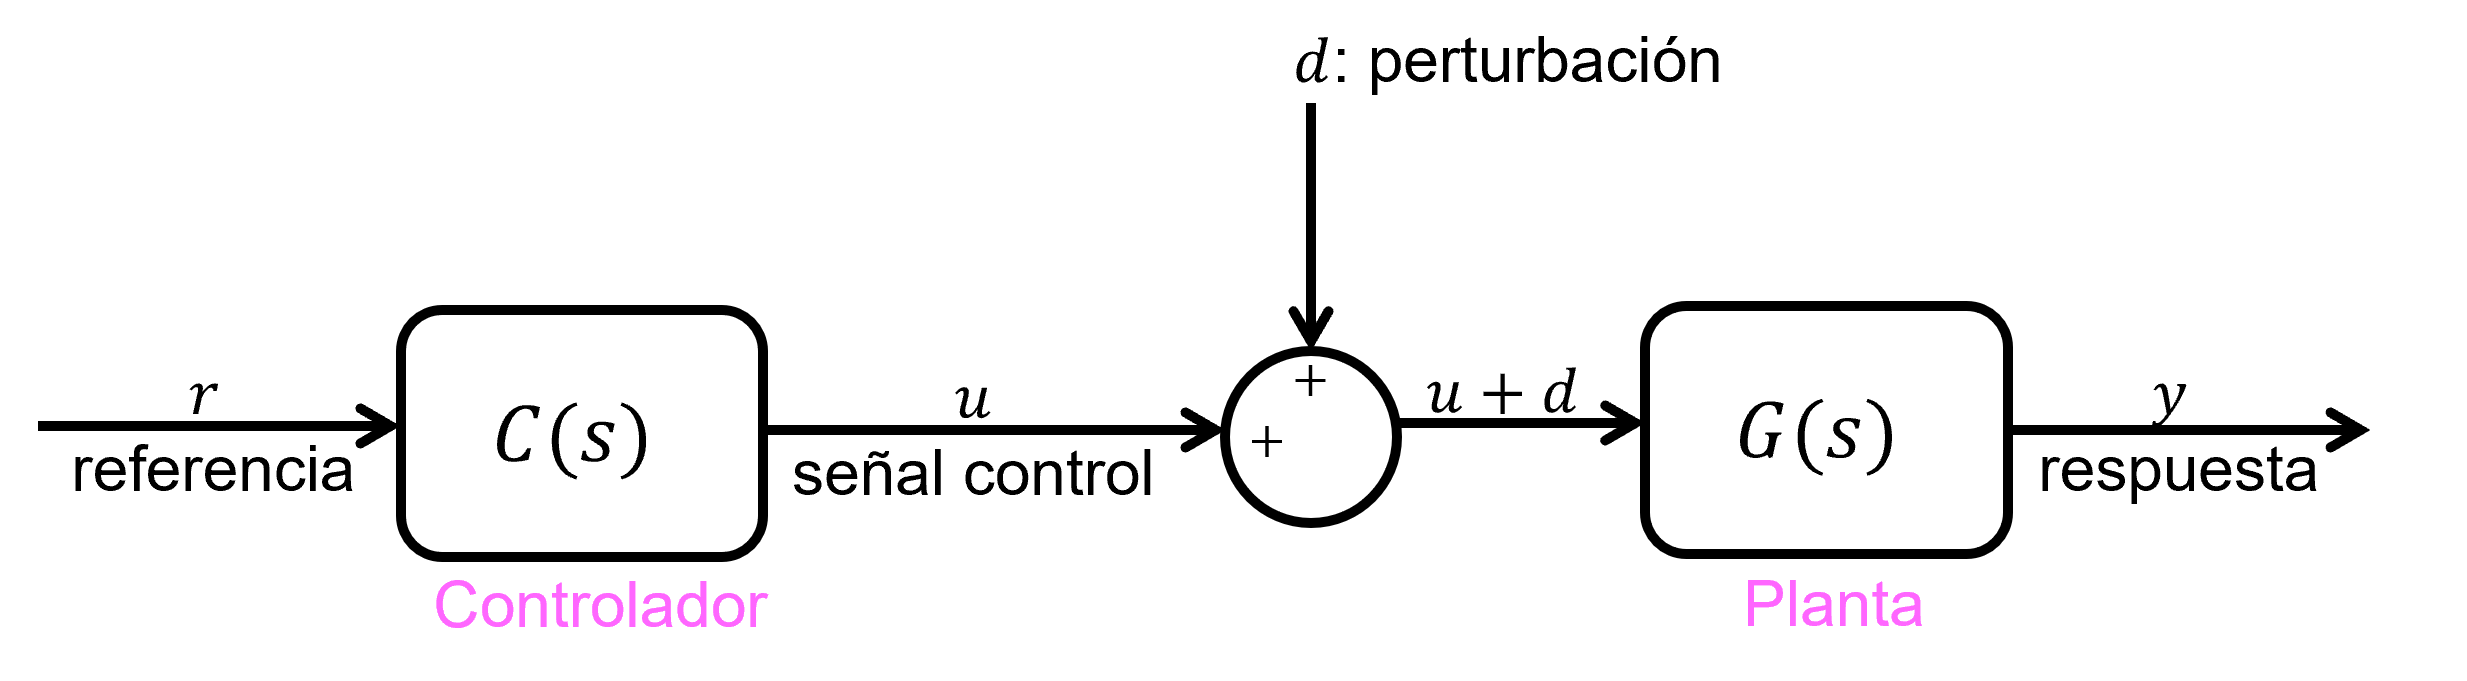
\includegraphics[scale=0.7]{Figuras/open-loop.png}
\end{figure}

\begin{itemize}
    \item[(1)] $Y(s)=G(s)[U(s)+D(s)]$, si asumimos $D(s)=0$
    \item[(2)] $U(s)=C(s)R(s)$
\end{itemize}

Reemplazar (2) en (1):
$$Y(s)=G(s)C(s)R(s)=L(s)R(s)$$
Donde $L(s)=G(s)C(s)$ es el sistema abierto ``open-loop system''.\\
\par Si buscamos: 
\begin{align*}
    y(t)&=r(t) ~/\color{red}{\mathcal{L}\{\cdot\}}\\
    Y(s)&=R(s)\\
    \Longrightarrow L(s)&=1\\
    \Longrightarrow C(s)&=\frac{1}{G(s)} ~\text{``control inverso''}
\end{align*}

\underline{Nota}: 
\begin{itemize}
    \item Muy simple y ``barato'' (no hay necesidad de sensores)
    \item No es robusto $\Longrightarrow$ si hay incertidumbre en $G(s)$
    \begin{align*}
        L(s)&=G(s)C(s)\neq 1\\
        &=[\hat{G}(s)+\Delta(s)]\frac{1}{\hat{G}(s)}\\
        &=1+\frac{\Delta(s)}{\hat{G}(s)}
    \end{align*}
\end{itemize}
\underline{Nota}: podría ser útil en RTHS, porque la respuesta es instantánea.

\subsection{Closed-loop (feedback) control}
\begin{figure}[H]
\centering
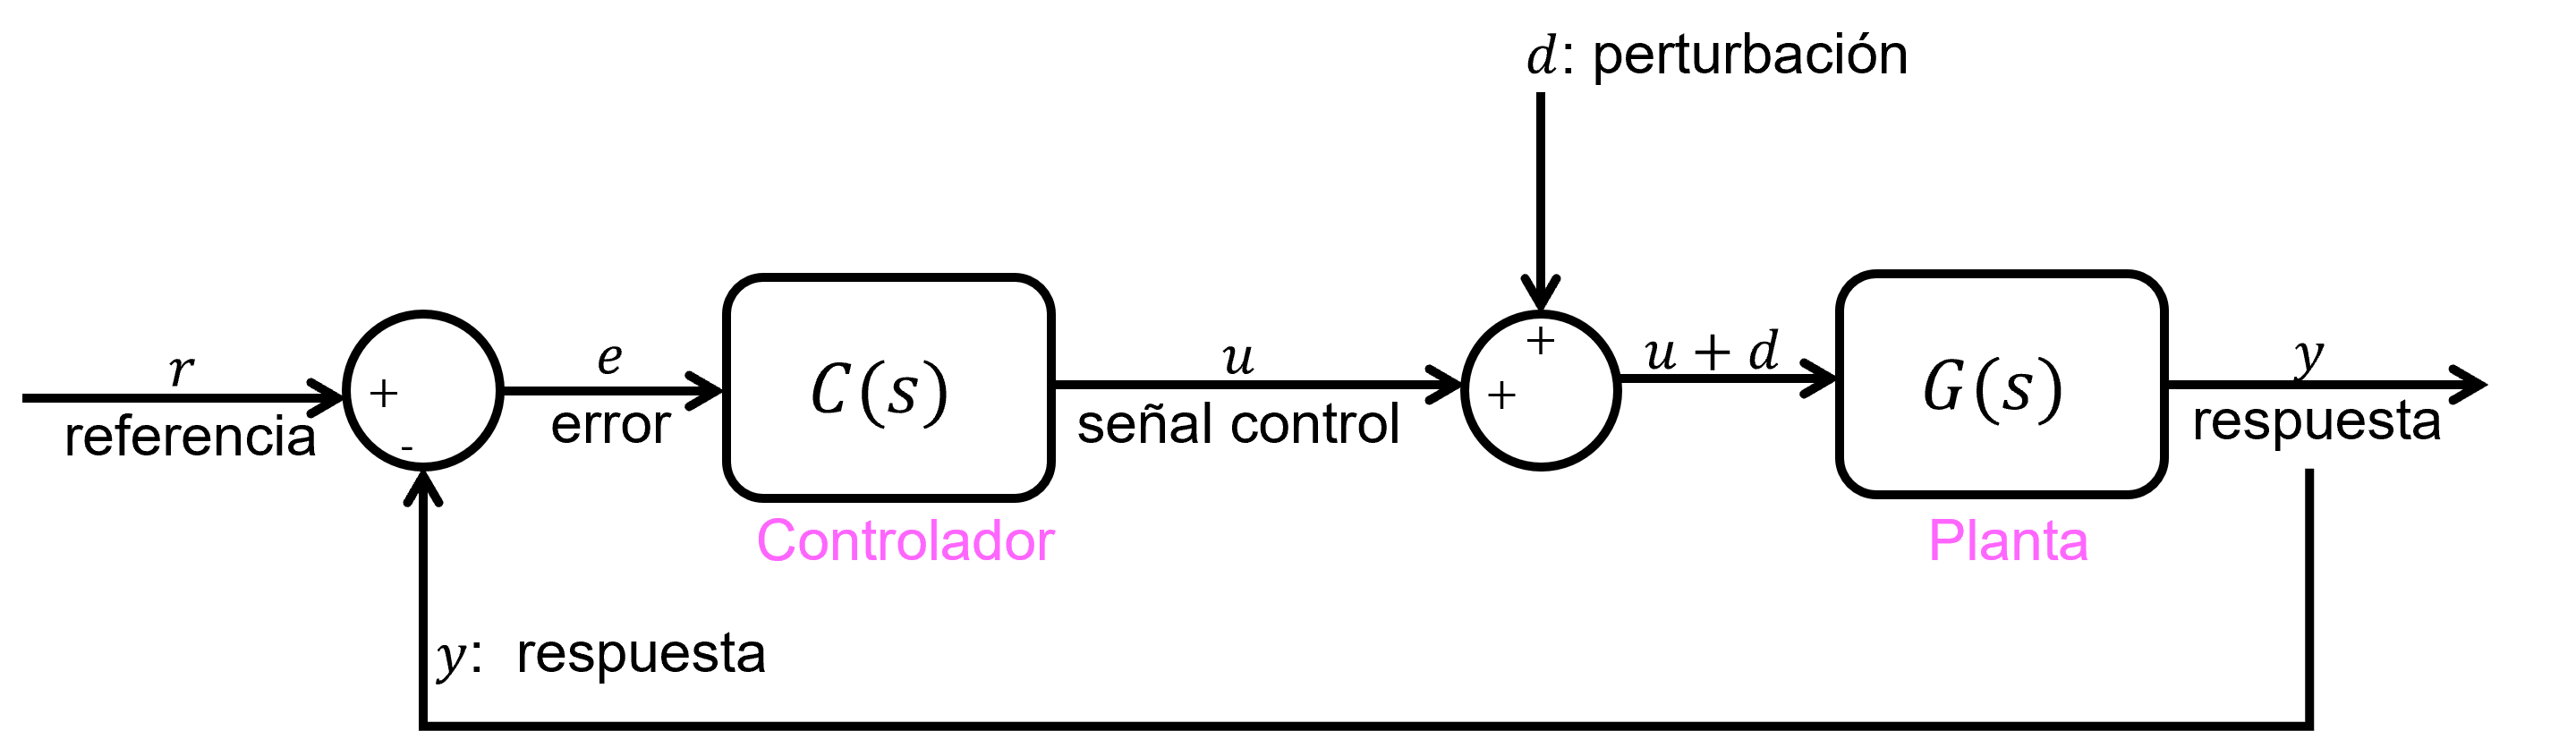
\includegraphics[scale=0.7]{Figuras/closed-loop.png}
\end{figure}

\begin{align*}
    \Longrightarrow & \text{Error: }~e(t)=r(t)-y(t)\\
    & \text{Si }e(t)=0\longrightarrow y(t)=r(t)
\end{align*}

\underline{Nota}:
\begin{itemize}
    \item Más robusto que feedforward $\Longrightarrow$ instalar sensores y ``alimentar'' la información de respuesta al controlador
    \item Más complicada y cara que open-loop
    \item Puede causar sistema estable o inestable
    \item Respuesta va a ser lenta $\Longrightarrow$ Real-time hybrid simulation
\end{itemize}

\section{Requisitos de control}
\begin{figure}[H]
\centering
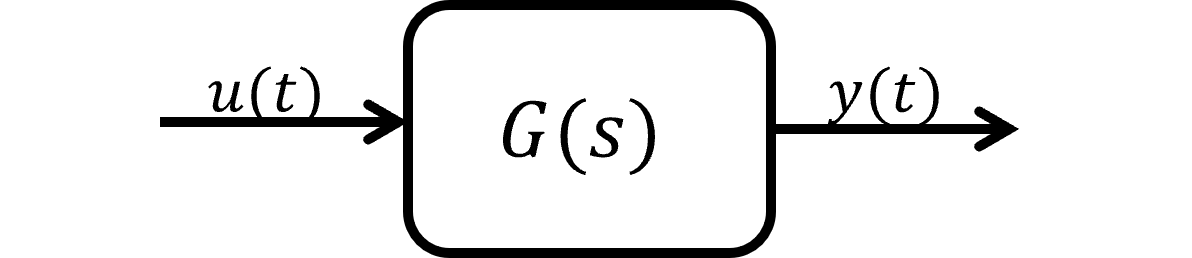
\includegraphics[scale=0.7]{Figuras/Planta.png}
\end{figure}
$\Longrightarrow$ Generar un set de requisitos de respuesta de planta $\Longrightarrow$ Especificaciones de respuesta transiente ante un escalón unitario
\begin{itemize}
    \item $t_r$ (tiempo de subida)
    \item $M_p$ (sobreimpulso)
    \item $t_s$ (tiempo de asentamiento)
\end{itemize}

\section{Diagrama de Bloque}
\begin{figure}[H]
\centering
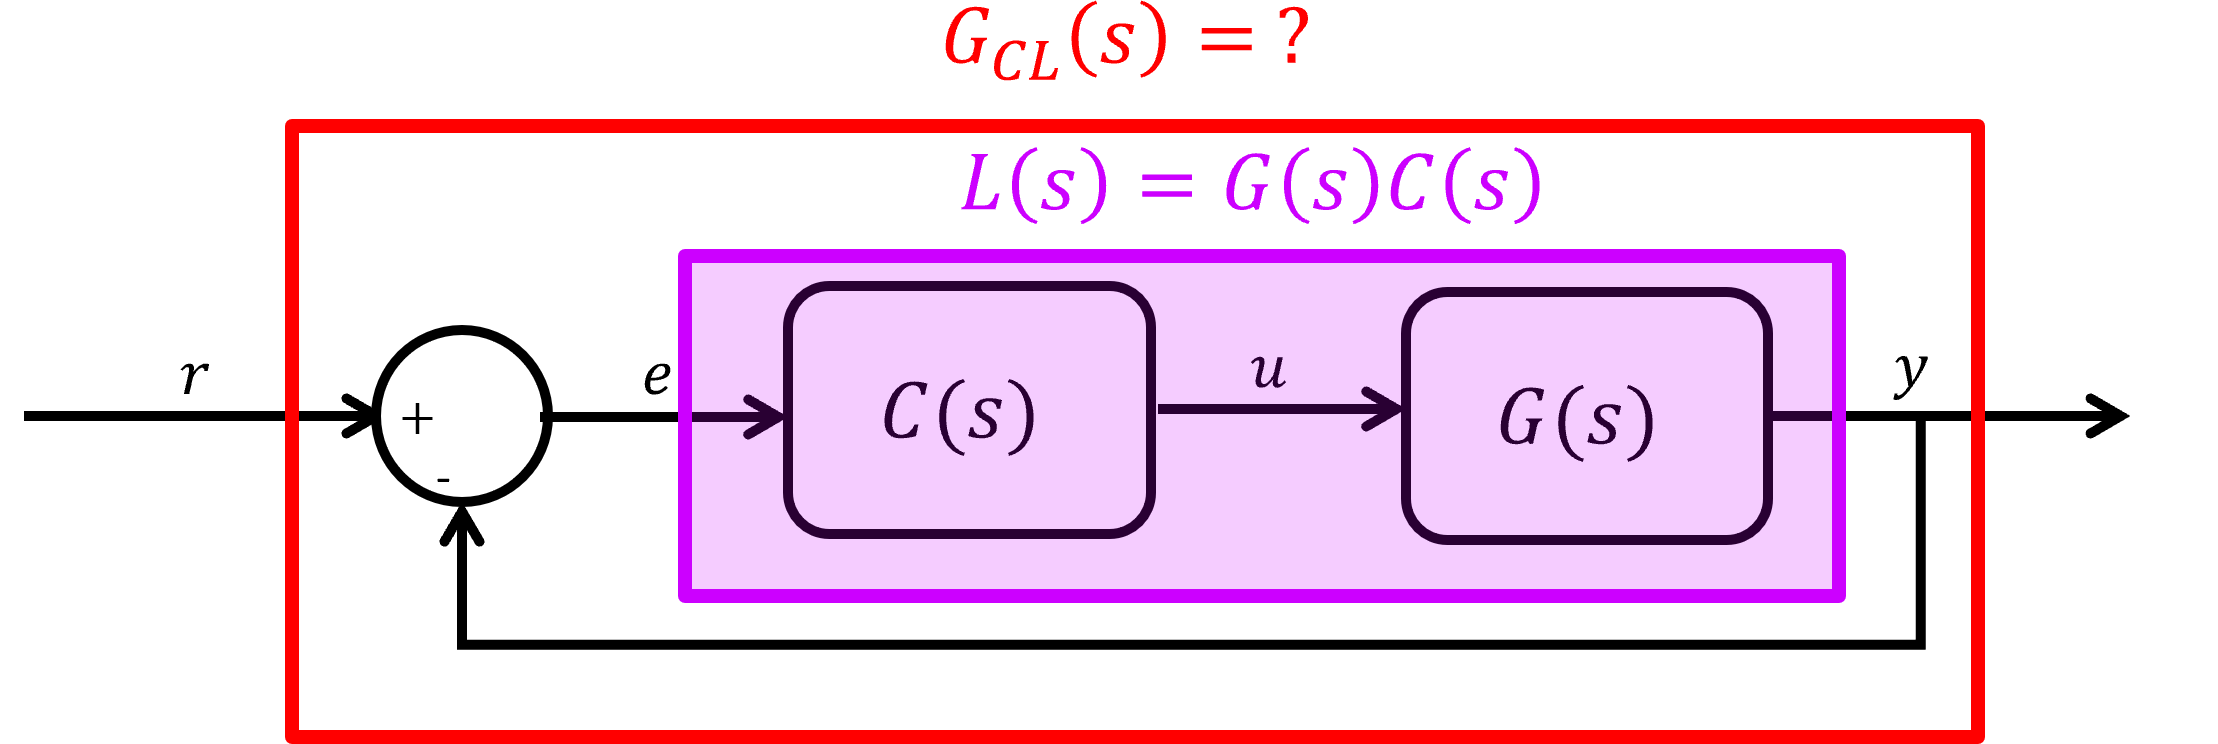
\includegraphics[scale=0.7]{Figuras/Diagrama_bloque.png}
\end{figure}
\begin{itemize}
    \item[(1)] $Y(s)=L(s)E(s)=G(s)C(s)E(s)$
    \item[(2)] $E(s)=R(s)-Y(s)$
\end{itemize}

(2) en (1): 
\begin{align*}
    \Longrightarrow Y(s)&=G(s)C(s)[R(s)-Y(s)]\\
    \Longrightarrow[1+G(s)C(s)]Y(s)&=G(s)C(s)R(s)\\
    \Longrightarrow Y(s)&= \bigg[\frac{G(s)C(s)}{1+G(s)C(s)}\bigg]R(s)\\
    \Longrightarrow Y(s)&= G_{CL}(s)R(s)
\end{align*}

\underline{Nota}: Vamos a ajustar $C(s)$ tal que $G_{CL}(s)$ tenga las propiedades deseadas en función de $t_r$, $M_p$ y $t_s$. O bien, elegir posición de los polos de $G_{CL}(s)$.





\section{Teorema Límite Final}
\begin{figure}[H]
\centering
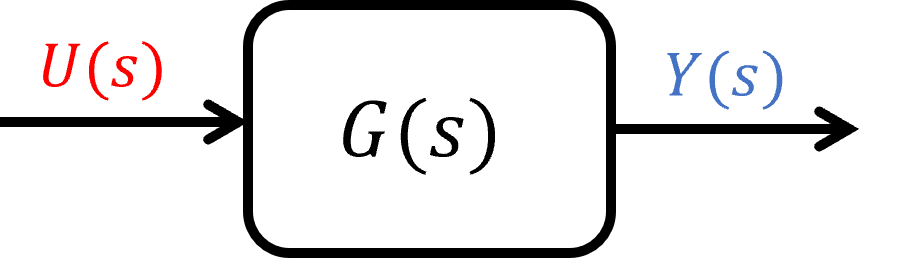
\includegraphics[scale=0.7]{Figuras/planta2.png}
\end{figure}
Respuesta Estado Estacionario: $y_\infty=\lim_{t\to\infty} y(t)$\\
\par Válido si y solo si $G(s)$ es estable.\\
\par \underline{Teorema}: Si todos los polos de $G(s)$ se encuentran a la izquierda del plano complejo, entonces:
\begin{align*}
    \lim_{t\to\infty} y(t)=\lim_{s\to 0} sY(s)
\end{align*}
\section{Sistema estructural con Active Mass Damper (AMD)}
\begin{figure}[H]
\centering
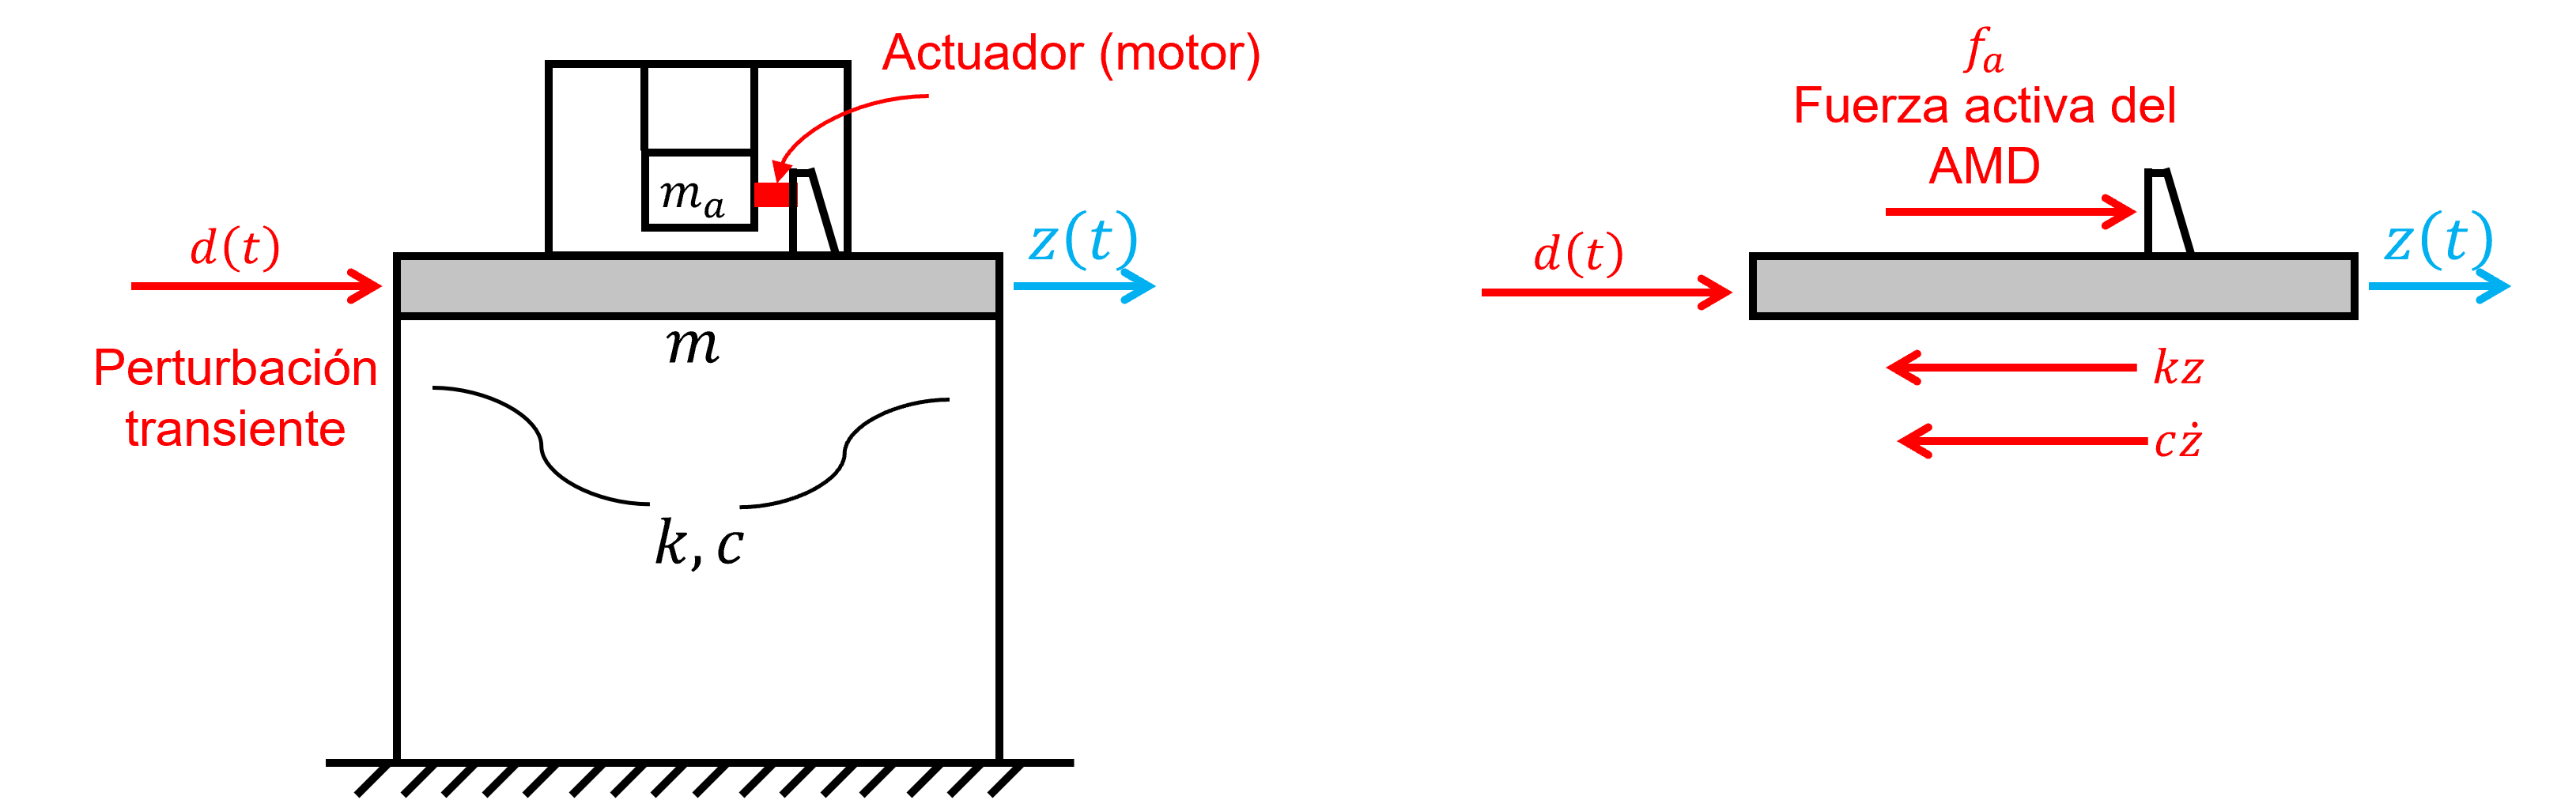
\includegraphics[scale=0.7]{Figuras/AMD.png}
\end{figure}
\begin{align*}
    \text{EDM: }~ m\ddot{z}+c\dot{z}+kz=f_a(u)+\cancelto{\text{Asuma=0}}{d}
\end{align*}
$u$: señal control (voltaje)\\
\par \underline{Objetivo}: Diseñar un \textcolor{red}{sistema de control} para mitigar $z(t)$ $\Longrightarrow$ Control PID (Proporcional-Integral-Derivativo)

\section{Control PID}
\begin{align*}
    C(s)=K_p+K_Ds+\frac{K_I}{s}
\end{align*}
\begin{itemize}
    \item $K_p$: control proporcional
    \item $K_D$: control derivativo
    \item $K_I$: control integral
\end{itemize}

\begin{figure}[H]
\centering
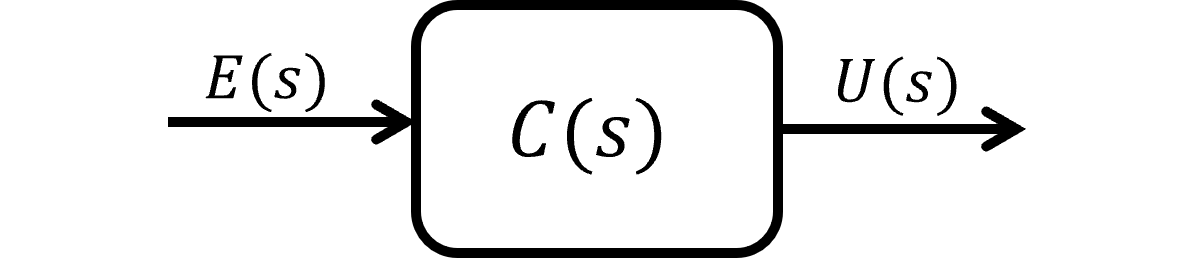
\includegraphics[scale=0.7]{Figuras/controlador.png}
\end{figure}

\begin{align*}
    U(s)&=C(s)E(s)\\
    &=K_pE(s)+K_DsE(s)+K_I\frac{E(s)}{s}~/\color{red}{\mathcal{L}^{-1}\{\cdot\}}\\
    \Longrightarrow u(t)&=K_pe(t)+K_D\frac{de(t)}{dt}+K_I\int e(t)dt
\end{align*}
 
\begin{itemize}
    \item $K_pe(t)$: error instantáneo
    \item $K_D\frac{de(t)}{dt}$: error futuro
    \item $K_I\int e(t)dt$: error pasado
\end{itemize}

\begin{figure}[H]
\centering
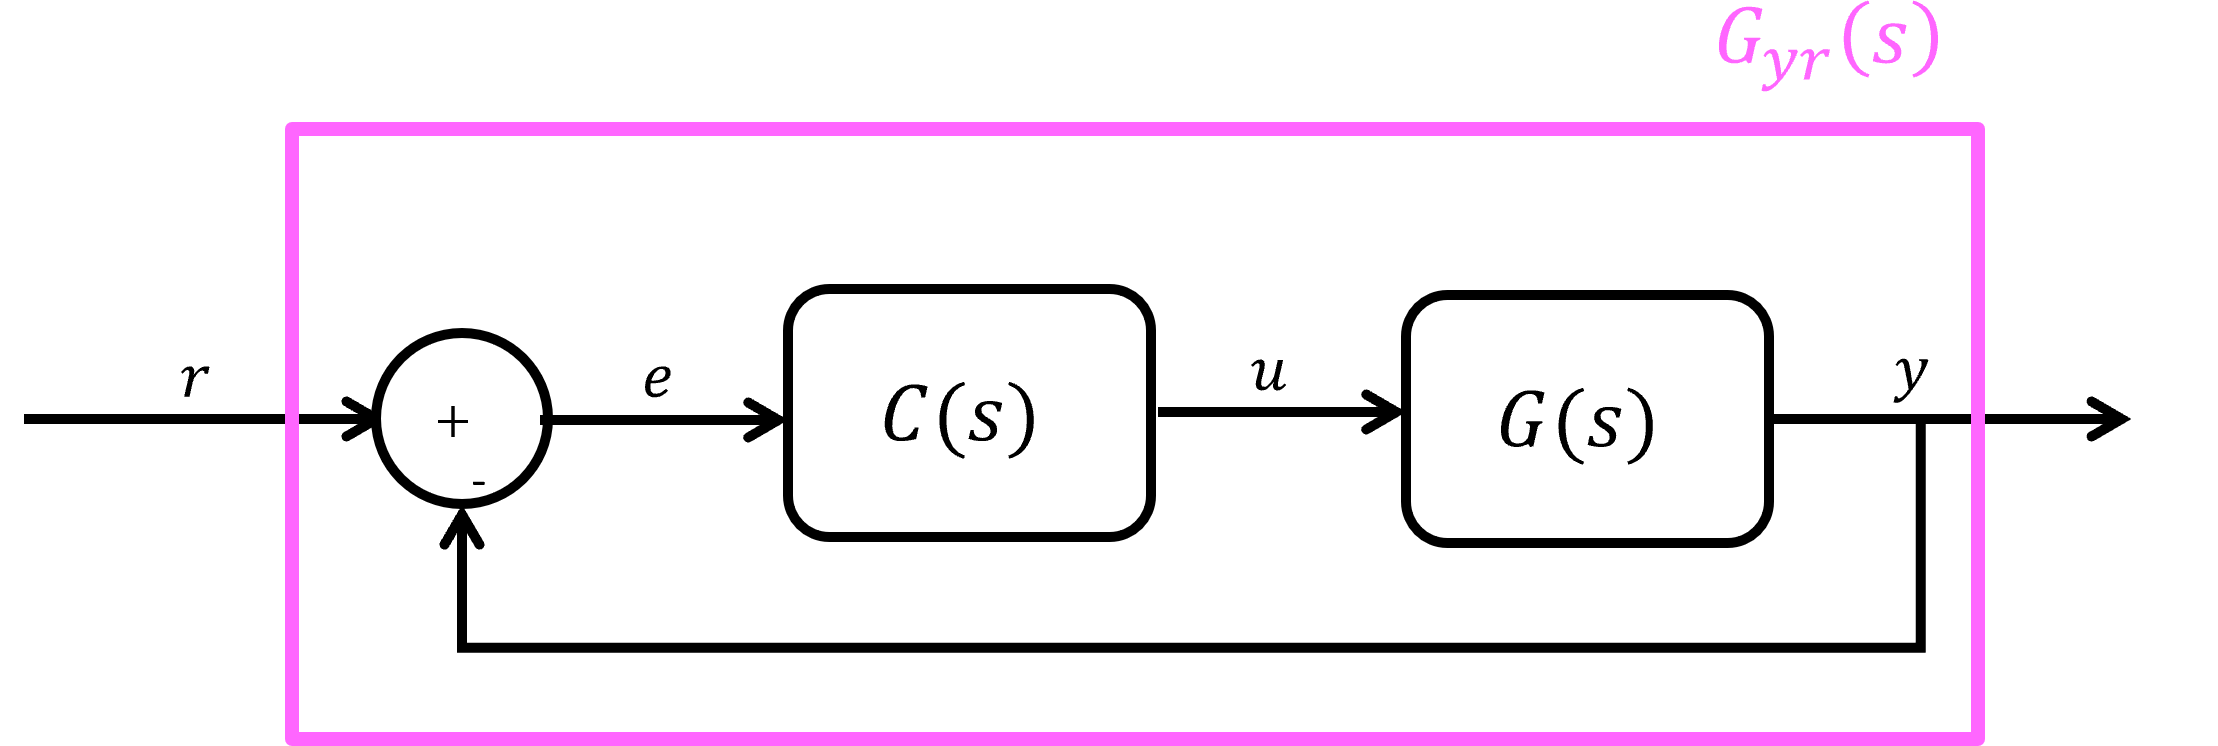
\includegraphics[scale=0.7]{Figuras/PID2.png}
\end{figure}
$C(s)$ se diseña tal que $e(t)\to 0$
$$C(s)=K_p+\frac{K_I}{s}+K_Ds$$
\begin{itemize}
    \item $Y(s)=G(s)U(s)$
    \item $U(s)=C(s)E(S)$
    \item $E(s)=R(s)-Y(s)$
\end{itemize}
\begin{align*}
    Y(s)&=G(s)C(s)[R(s)-Y(s)]\\
    \Longrightarrow Y(s)&=\frac{G(s)C(s)}{1+G(s)C(s)}R(s)\\
    &=G_{CL}R(s)\\
    &=G_{yr}R(s)
\end{align*}

\subsection{Control Proporcional (P)}
\begin{align*}
    & C(s)=K_p\\
    \Longrightarrow & G(s)=\frac{1}{ms^2+cs+k}=\frac{1/m}{s^2+2\xi\omega_n s+\omega_n^2}=\frac{c}{s^2+as+b}\\
    \Longrightarrow & G_{CL}(s)=\frac{K_p\frac{c}{s^2+bs+c}}{1+K_p\frac{c}{s^2+bs+c}}
\end{align*}
\begin{align*}
    \Longrightarrow & G_{CL}(s)=\frac{K_p c}{s^2+as+(b+K_p\cdot c)}\\
    \Longrightarrow & \omega_{n,CL}= \sqrt{b+K_p\cdot c}\\
    \Longrightarrow & \xi_{CL}= \frac{a}{2\omega_{n,CL}}=\frac{a}{2\sqrt{b+K_p\cdot c}}
\end{align*}
\begin{itemize}
    \item Aumentar $K_p$ hace que $\omega_{n,CL}$ aumente (sistema rígido)
    \item Aumentar $K_p$ hace que $\xi$ disminuya
\end{itemize}

En términos de la respuesta $y_{\infty}$: 
\begin{align*}
    y_{\infty}=\lim_{s\to 0}sY_{CL}(s)=\lim_{s\to 0} sG_{CL}(s)R(s)
\end{align*}
Con $R(s)$: escalón unitario

\begin{align*}
    \Longrightarrow y_{\infty}=\lim_{s\to 0} s\frac{K_p\cdot c}{s^2+as+(b+K_p\cdot c)}\cdot\frac{1}{s}=\frac{K_p\cdot c}{b+K_p \cdot c}\neq 1
\end{align*}
Valores pequeños de $K_p\Longrightarrow$ error en estado estacionario
\begin{figure}[H]
\centering
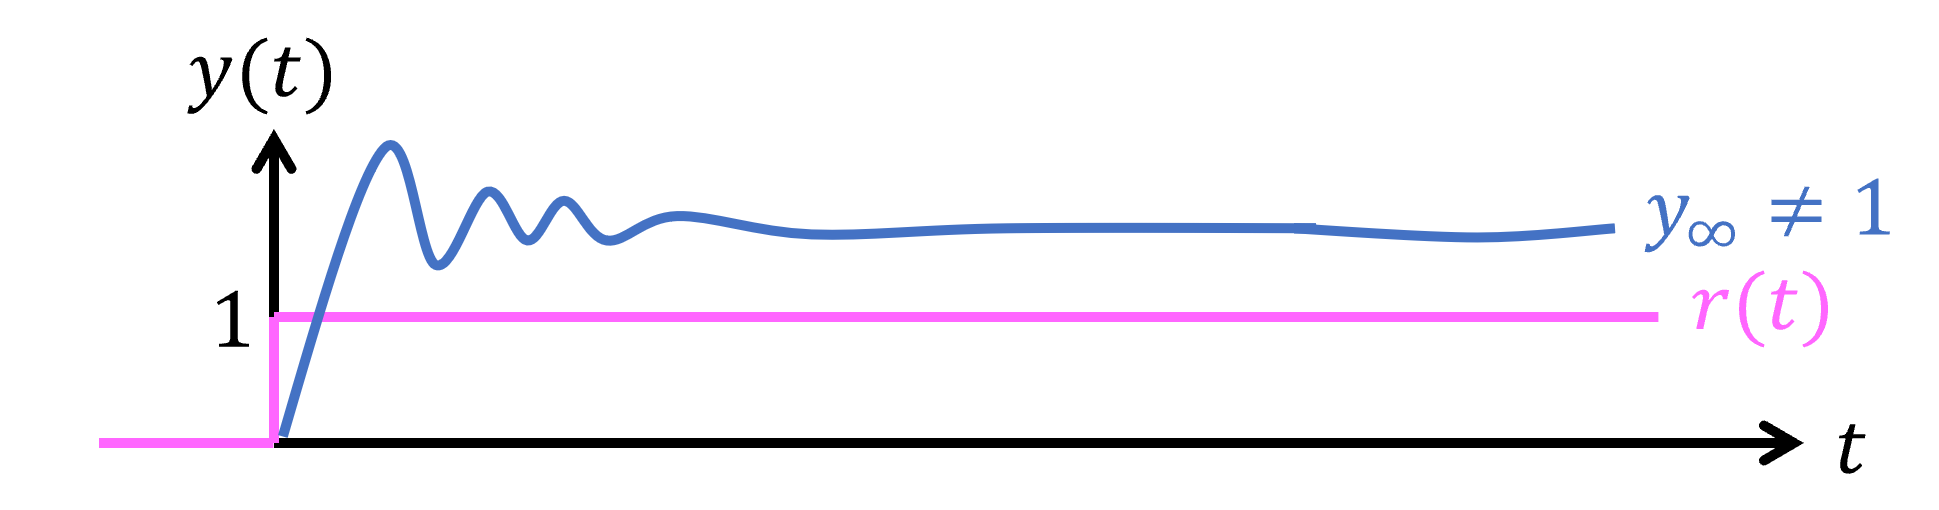
\includegraphics[scale=0.7]{Figuras/controlP.png}
\end{figure}

\subsection{Control PD}
\begin{align*}
    G_{CL}(s)&=\frac{G(s)C(s)}{1+G(s)C(s)}=\frac{\left(\frac{c}{s^2+as+b}\right)C(s)}{1+\left(\frac{c}{s^2+as+b}\right)C(s)}\\
    & = \frac{c\cdot C(s)}{a^2+as+\left( b+c \cdot C(s) \right)}\\
    C(s) &= K_p+K_Ds=K_p(1+T_Ds)\\
    \Longrightarrow G_{CL} &= \frac{cK_p(1+T_Ds)}{s^2+(a+cbK_pT_D)s+b(1+K_p)}
\end{align*}

\begin{itemize}
    \item Aparece un ``cero'' en el numerador
    \item Podemos controlar $\omega_{n,CL}$ mediante $K_p$
    \item Podemos controlar $\xi_{CL}$ mediante una combinación de $K_p$ y $T_D$
\end{itemize}

$\Longrightarrow y_{\infty}$, no hay cambio en el error de estado estacionario\\
\par $\Longrightarrow$ Con PD podemos ubicar los polos del sistema cerrado donde nosotros queramos\\
\par \underline{Advertencia}: Control D amplifica el ruido eléctrico en la señal de respuesta $\Longrightarrow$ Nunca utilizar control D.

\subsection{Control PI}
\begin{align*}
    \Longrightarrow G_{CL}(s) &= \frac{c\cdot C(s)}{s^2+as+\left(b+c \cdot C(s)\right)}\\
    \Longrightarrow C(s) &= K_p +\frac{K_I}{s}=K_P\left(1+\frac{T_I}{2}\right)\\
    \Longrightarrow G_{CL} &= \frac{cK_p(s+T_I)}{s^3+as^2+(b+cK_p)s+cK_pT_I}
\end{align*}

\begin{align*}
    \Longrightarrow y_{\infty}=\lim_{s\to 0}sY_{CL}(s)=\lim_{s\to 0} s\frac{K_p\cdot c(s+T_I)}{s^3+as^2+(b+cK_p)s+cK_pT_I}\cdot\frac{1}{s}=\frac{T_IK_p\cdot c}{T_IK_p\cdot c}= 1
\end{align*}

\underline{Nota}: El esfuerzo del control I genera una reducción del error en estado estacionario.

\subsection{Control PID}
\begin{align*}
    C(s) &= K_p+\frac{K_I}{s}+K_Ds\\
    &= K_p\left(1+\frac{T_I}{s}+T_Ds\right)
\end{align*}

\begin{itemize}
    \item Aumentar $K_p$: Sistema que responde rápido, pero se genera alto sobreimpulso, y el error estacionario alto.
    \item Aumentar $K_D$: Agregar amortiguameinto al sistema (disminuir sobreimpulso), pero puede amplificar el ruido eléctrico.
    \item Aumentar $K_I$: Reducir el error en estado estacionario, sistema se vuelve más lento.
\end{itemize}

\begin{table}[H]
    \centering
    \begin{tabular}{c|c|c|c|}
                & $K_p \uparrow$ & $K_D \uparrow$ & $K_I \uparrow$\\ \hline
         error ss & $\downarrow$ & - & 0\\ \hline
         $t_r$ & $\downarrow$ & - & ? \\ \hline
         $t_s$ & - & $\downarrow$ & ? ($\uparrow$)\\ \hline
         $M_p$ & $\uparrow$ & $\downarrow$ & ? ($\uparrow$)\\ 
    \end{tabular}
\end{table}



\section{Ejemplo: Simulación mediante Simulink}
\begin{figure}[H]
\centering
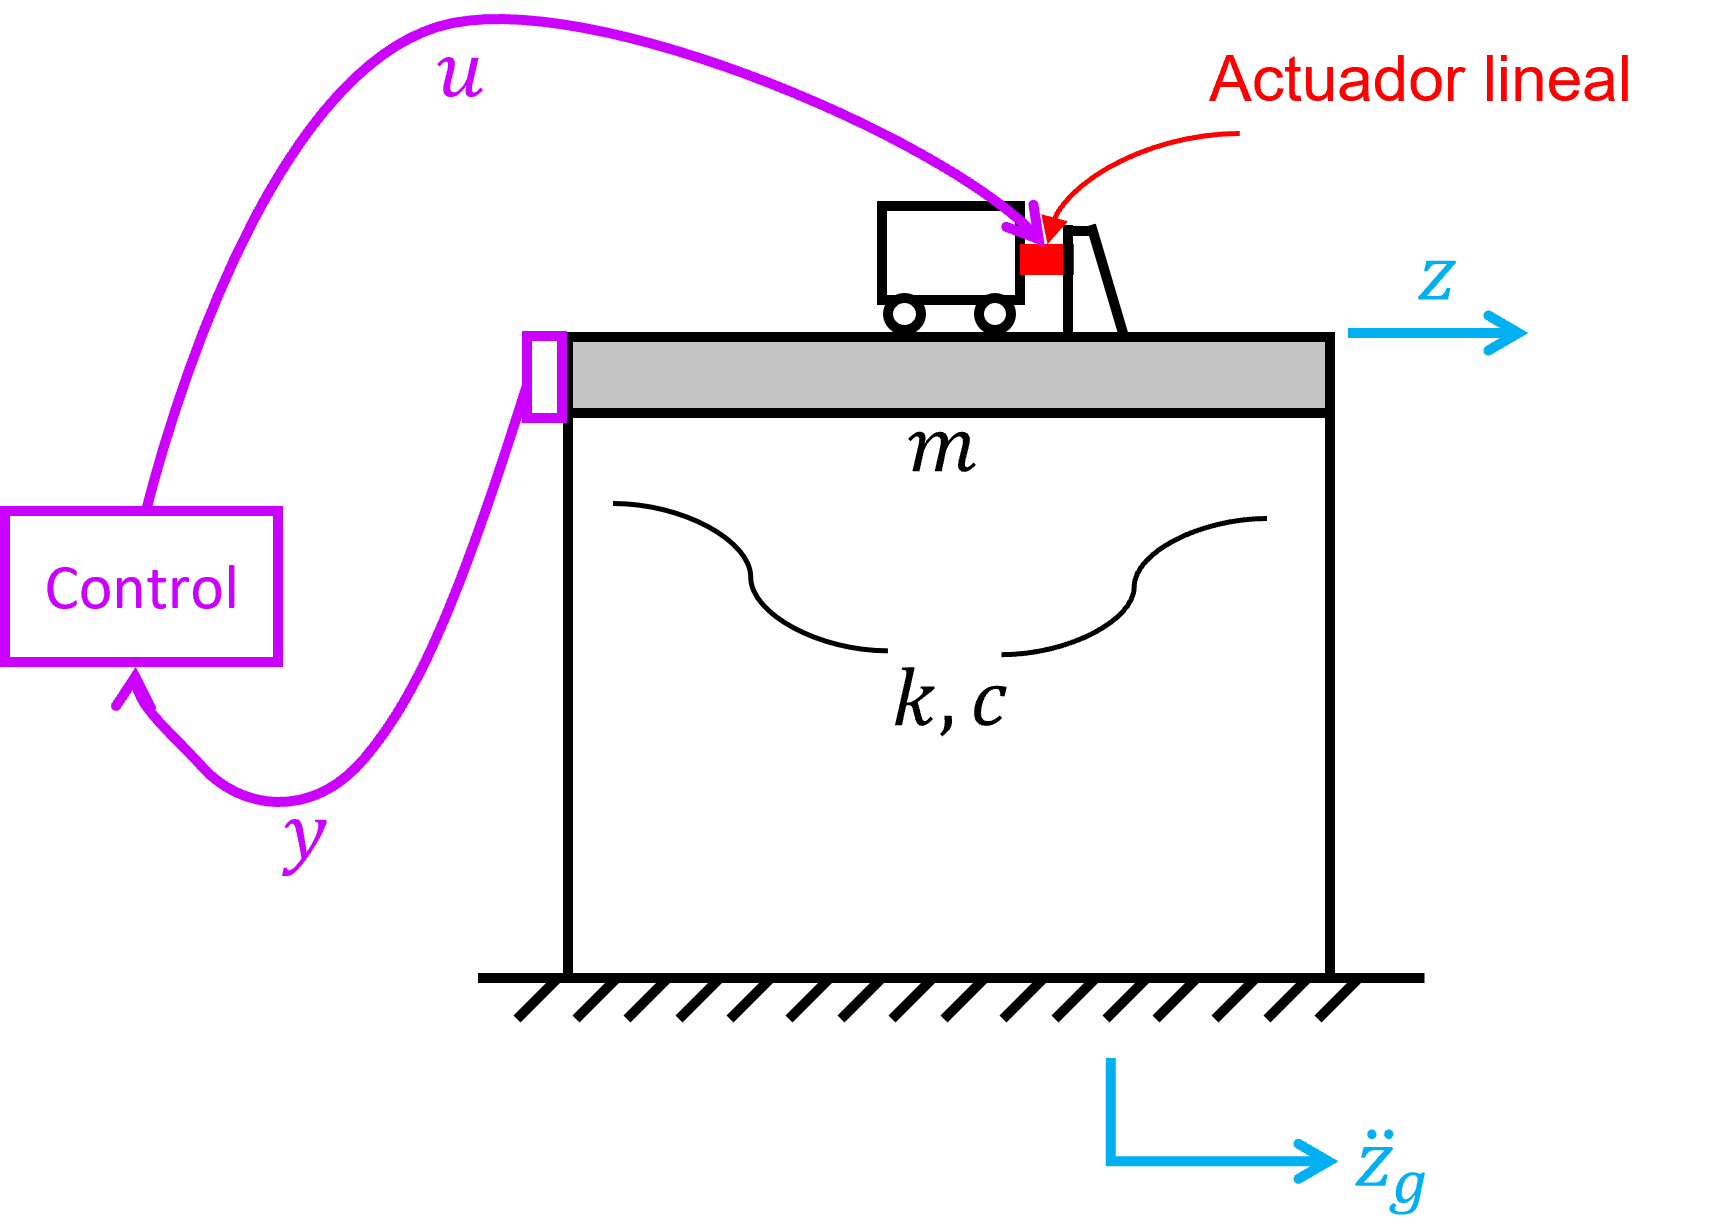
\includegraphics[scale=0.7]{Figuras/simulink_modelo.png}
\end{figure}

\begin{align*}
    \text{EDM: }~ m\ddot{z}+c\dot{z}+kz=-m\ddot{z}_g+gu
\end{align*}

\underline{Propiedades de la estructura}: 
\begin{itemize}
    \item $m=100$ Kg
    \item $c=50$ Ns/m
    \item $k=4000$ N/m
    \item $g=100$ N/V
\end{itemize}

\underline{Representación espacio-estado}: 
\begin{align*}
    \tend{x}=\begin{bmatrix}\tend{z}\\ \tend{\dot{z}}\end{bmatrix}, \quad u_1 =\ddot{z}_g, \quad u_2=u
\end{align*}

\begin{align*}
    \tend{\dot{x}} &=
    \begin{bmatrix}
    0 & 1\\
    -k/m & -c/m
    \end{bmatrix}\tend{x} +
    \begin{bmatrix}
    0 \\ -1
    \end{bmatrix}u_1+
    \begin{bmatrix}
    0 \\ g/m
    \end{bmatrix}u_2 \\
    &= \begin{bmatrix} 0 & 1\\-k/m & -c/m
    \end{bmatrix}\tend{x} +
    \begin{bmatrix}
    0 & 0\\ -1 & g/m
    \end{bmatrix} 
    \begin{bmatrix}
    \ddot{z}_g\\ u
    \end{bmatrix}
\end{align*}

\begin{align*}
    \tend{y}&=[z]\\
    \tend{y}&= \begin{bmatrix}1 & 0 \end{bmatrix}\tend{x}+\begin{bmatrix}0 & 0 \end{bmatrix}\begin{bmatrix}
    \ddot{z}_g\\ u
    \end{bmatrix}
\end{align*}

\begin{align}
    \tend{u}=\begin{bmatrix}
    \ddot{z}_g\\ u
    \end{bmatrix}\longrightarrow
    \begin{array} {|r|r|}
      \hline A & B \\
      \hline C & D \\
      \hline 
    \end{array}
    \longrightarrow \tend{y}=[z] \quad \text{Sistema ``MISO''}
\end{align}


\underline{Objetivo}: Diseñar un control PID para mejorar el desempeño de la estructura sometida al terremoto de Northridge 1994.\\
\par \underline{Contol PID}: 
\begin{align*}
    C(s)&=K_p\bigg(1+\frac{T_I}{s}+T_Ds\bigg)\\
    &= K_p+\frac{K_I}{s}+K_Ds, \quad K_I=K_pT_I, \quad K_D=K_pT_D
\end{align*}

\begin{multicols}{2}
\underline{Código Matlab}: 
\begin{minted}[]{matlab}
%% Simulacion Control PID
% Gaston Fermandois, 2020

%% Inicializar
clear all, close all, clc

%% Parametros

m=100; % masa primer piso, kg
c=50; %Ns/m
k=4000; %N/m
g=100; %cte motor, N/V

%% Control PID

Kp=1;
Ti=1/10; Ki=Kp*Ti;
Td=1/100; Kd=Kp*Td;

s=tf('s');
Cpid=Kp*(1+Ti/s+Td*s);

%% Espacio estado

A=[0 1;-k/m -c/m];
B1=[0;-1];
B2=[0;g/m];
B=[B1 B2];
C=[1 0];
D1=0;
D2=0;
D=[D1 D2];

sys=ss(A,B,C,D);

sysyu=ss(A,B2,C,D2);

Gyu=tf(sysyu);

%% Sistema Cerrado

Gcl=Gyu*Cpid/(1+Gyu*Cpid);
Gcl=minreal(Gcl)

figure;
rlocus(Gcl)

%% Simulacion

Tfinal=60; %s
Fs=1000; %Hz
Ts=1/Fs; %s

GM=importdata('RegistroNorthridge1994.txt');
N=length(GM.data);
dt=0.02; %s
t=linspace(0,N*dt,N);
ddzg=[t.' GM.data/100]; %[s m/s2]

sim('AMDctrl_demo_simu')
\end{minted}
\end{multicols}
\underline{Simulink}:
\begin{figure}[H]
\centering
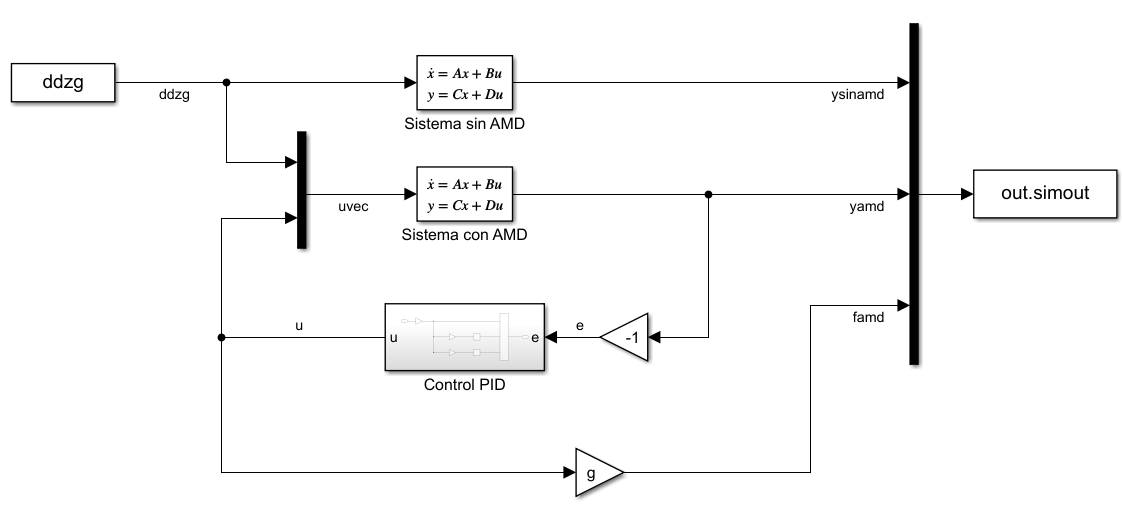
\includegraphics[scale=0.7]{Figuras/Simulink.png}
\end{figure}



\section{Root Locus}
$\Longrightarrow$ ``Migración de polos'', Locus = posición en latín
\begin{align*}
    \text{Planta: }~ G_{y\ddot{z}_g}(s)&=\frac{1/m}{s^2+2\xi\omega_n s+\omega_n^2}\\
    G_{yu}(s) &=\frac{g/m}{s^2+2\xi\omega_n s+\omega_n^2}
\end{align*}
\begin{align*}
    \text{Controlador PID: }~C(s)=K_p(1+\frac{T_I}{s}+T_Ds)
\end{align*}

\begin{figure}[H]
\centering
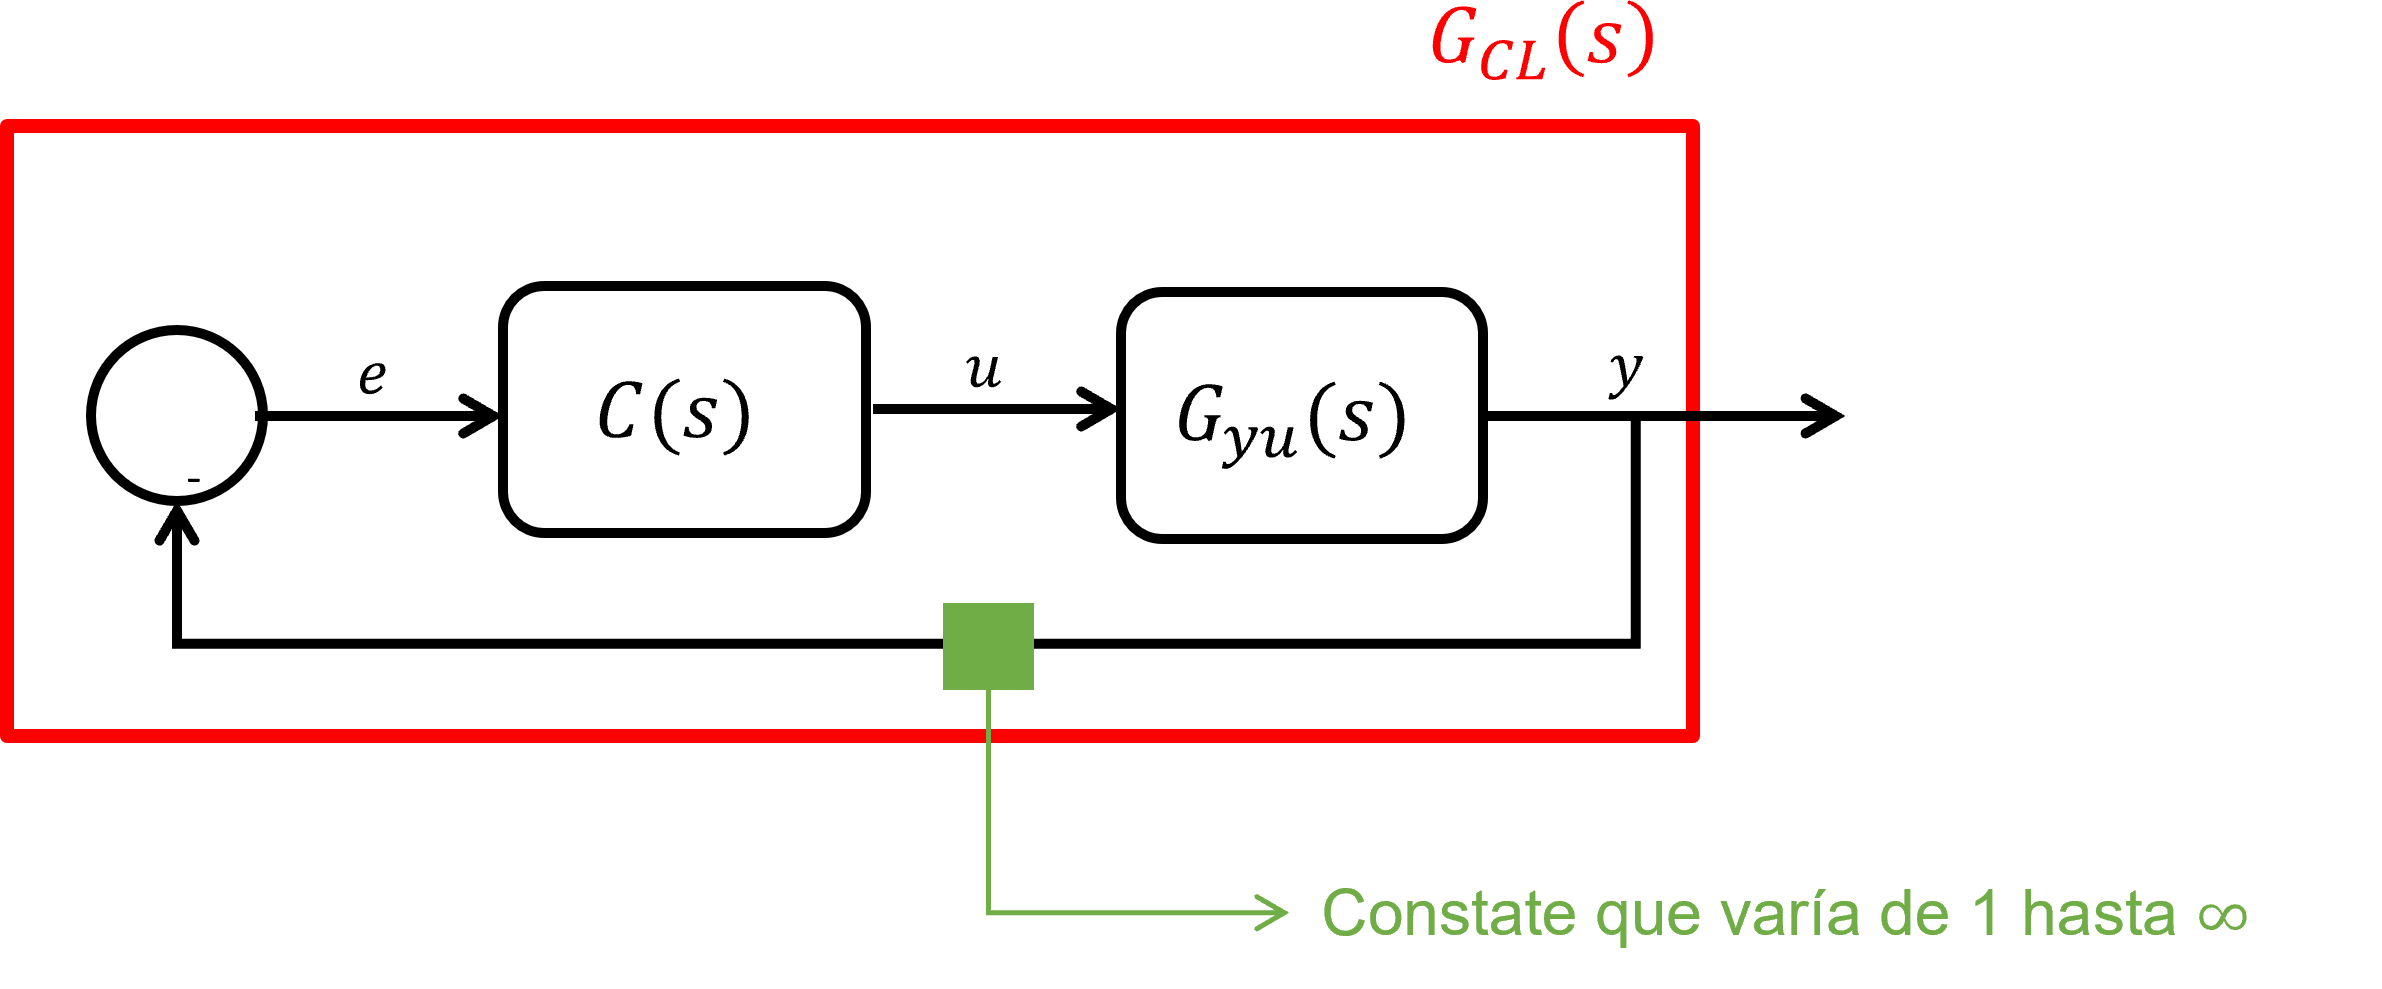
\includegraphics[scale=0.7]{Figuras/GCL.png}
\end{figure}

\begin{align*}
    G_{CL}(s)&=\frac{G(s)C(s)}{1+G(s)C(s)}\\
    G_{CL}(s)&=\frac{G(s)K_p\bigg(1+T_I/s+T_Ds\bigg)}{1+G(s)K_p\bigg(1+T_I/s+T_Ds\bigg)}
\end{align*}

\underline{Resumen control PID}: 
\begin{figure}[H]
\centering
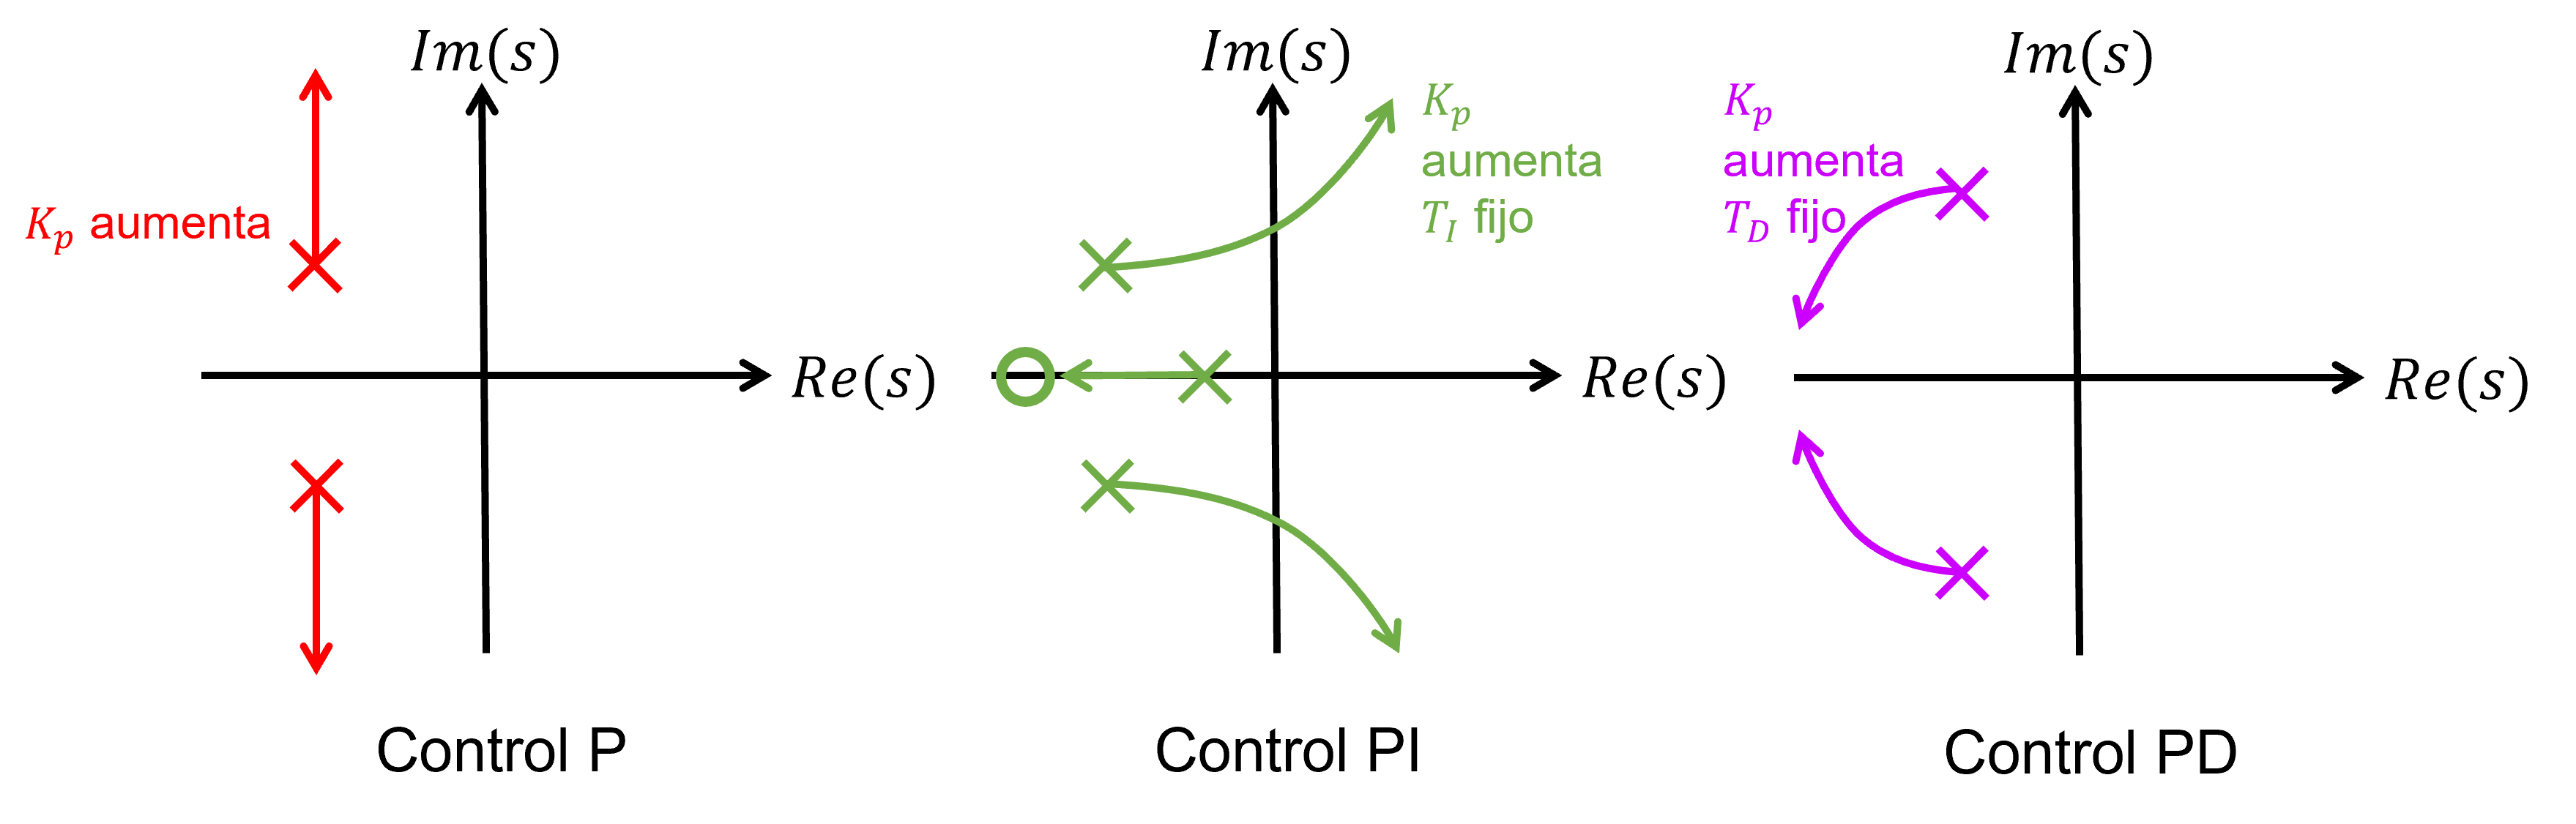
\includegraphics[scale=0.65]{Figuras/controlPID.png}
\end{figure}

\section{Control Moderno}
Representación espacio estado, sistema LTI.\\
\par Sea: 
\begin{align*}
    \tend{x}&=[x_1,x_2,...,x_N]^\top\\
    \tend{u}&=[u_1,u_2,...,u_p]^\top\\
    \tend{y}&=[y_1,y_2,...,y_r]^\top
\end{align*}
\begin{itemize}
    \item[(1)] Ecuación de estado:
    $$\tend{\dot{x}}=\tenq{A}\tend{x}+\tenq{B}\tend{u} $$
    \item[(2)] Ecuación de respuesta:
    $$\tend{y}=\tenq{C}\tend{x}+\tenq{D}\tend{u} $$
\end{itemize}

\underline{Paréntesis}:
\begin{align*}
    \tend{X}(s)&=\mathcal{L}\{\tend{x}(t)\}\\
    \tend{U}(s)&=\mathcal{L}\{\tend{u}(t)\}\\
    \tend{Y}(s)&=\mathcal{L}\{\tend{y}(t)\}
\end{align*}
\begin{align*}
    \tend{\dot{x}}\tenq{A}\tend{x}+\tenq{B}\tend{u}\xrightarrow[]{\mathcal{L}}s\tend{X}(s)=\tenq{A}\tend{X}(s)+\tenq{B}\tend{U}(s)\\
    \Longrightarrow \tend{X}(s)=(s\tenq{I}-\tenq{A})^{-1}\tenq{B}\tend{U}(s)\\
    G_{xu}(s)=(s\tenq{I}-\tenq{A})^{-1}\tenq{B}
\end{align*}
\begin{align*}
    \tend{y}=\tenq{C}\tend{x}+\tenq{D}\tend{u}\xrightarrow[]{\mathcal{L}}s\tend{Y}(s)=\tenq{C}\tend{X}(s)+\tenq{D}\tend{U}(s)\\
    \tenq{Y}(s)=[\tenq{C}(s\tenq{I}-\tenq{A})^{-1}\tenq{B}+\tenq{D}]\tend{U}(s)\\
    G_{yu}=\tenq{C}(s\tenq{I}-\tenq{A})^{-1}\tenq{B}+\tenq{D}
\end{align*}


\section{Formas canónicas}
\subsection{Forma Canónica Controlable (CCF)}
Asumir que $\tenq{D}=\tenq{0}$ (no hay componente ``feedthrough'' en la salida del sistema).
\begin{align*}
\tenq{A_c}=\left[
    \begin{array}{cccc|c}
     -a_1 & -a_2 & \dots & -a_{n-1} & -a_n\\ \hline
     1 & & & 0 & 0\\
       & 1 & & & \vdots\\
       & & \ddots & & \\
     0 & & & 1 & 0  
    \end{array}\right], \quad \tenq{A_c}\in \mathbb{R}^{n\times n}
\end{align*}
\begin{align*}
\tenq{B_c}=\left[
    \begin{array}{c}
     1 \\ \hline
     0\\
    \vdots\\
     0  
    \end{array}\right], \quad \tenq{B_c}\in \mathbb{R}^{n\times 1}
\end{align*}
\begin{align*}
\tenq{C_c}=\left[
    \begin{array}{cccc}
     b_1 & b_2 & \dots & b_n
    \end{array}\right], \quad \tenq{C_c}\in \mathbb{R}^{1\times n}
\end{align*}
\begin{align*}
    \text{Realización (SISO): }\quad 
    \left\{
    \begin{array}{l}
          \tend{\dot{x}_c}=\tenq{A_c}\tend{x_c}+\tenq{B_c}u \\
          y=\tenq{C_c}\tend{x_c} \\
    \end{array} 
    \right. 
\end{align*}
Notar que:
\begin{align*}
    \dot{x}_1 &= -a_1x_1-a_2x_2 ... -a_nx_n+1\cdot u\\
    \dot{x}_2 &= x_1\\
    \dot{x}_3 &= x_2\\
    \vdots \\
    \dot{x}_n &= x_{n-1}
\end{align*}

Utilizando la transformada de Laplace, se obtiene la siguiente función de transferencia:
\begin{align*}
    G_{yu}(s)=\frac{b_1s^{n-1}+b_2s^{n-2}+...+b-n}{s^n+a_1s^{n-1}+a_2s^{n-2}+...+a_n} = \frac{\text{numerador orden n-1}}{\text{denominador orden n}} = \text{TF Propia}
\end{align*}

Se utiliza para diseñar controladores cuando todos los estados del sistema son conocidos.

\subsection{Forma Canónica Modal (MCF)}
Sea $G(s)=\frac{c_1}{s+p_1}+\frac{c_2}{s+p_2}+...+\frac{c_n}{s+p_n}$, $G(s)$ se escribe como una expansión de fracción parcial, y los polos $p_i$ son todos distintos:
\begin{align*}
\tenq{A_m}=\left[
    \begin{array}{cccc}
     -p_1& & & 0\\
     & -p_2 & & \\
     & & \ddots & \\
     0 & & & -p_n
    \end{array}\right], \quad \tenq{A_m}\in \mathbb{R}^{n\times n}
\end{align*}
\begin{align*}
\tenq{B_m}=\left[
    \begin{array}{c}
     1 \\ 
     1\\
    \vdots\\
     1  
    \end{array}\right], \quad \tenq{B_m}\in \mathbb{R}^{n\times 1}
\end{align*}
\begin{align*}
\tenq{C_m}=\left[
    \begin{array}{cccc}
     c_1 & c_2 & \dots & c_n
    \end{array}\right], \quad \tenq{C_m}\in \mathbb{R}^{1\times n}
\end{align*}

\begin{align*}
    \text{Realización (SISO): }\quad 
    \left\{
    \begin{array}{l}
          \tend{\dot{x}_m}=\tenq{A_m}\tend{x_m}+\tenq{B_m}\cancelto{0}{u} 
    \end{array} 
    \right. 
\end{align*}

\begin{align*}
    \dot{x}_{m_1} &= \lambda_1x_{m_1}\\
    \dot{x}_{m_2} &= \lambda_2x_{m_1}\\
    \vdots \\
    \dot{x}_{m_n} &= \lambda_nx_{m_n}
\end{align*}

\begin{align*}
    \Longrightarrow\tend{\dot{x}}=\tenq{A}\tend{x}
\end{align*}

\underline{Resolver}: $\tenq{A}\tend{v}=\lambda \tend{v}$ (Problema de valores propios de $\tenq{A}$).\\
\par $\tenq{T}$ es la matriz de transformación modal, $\tenq{T}=[\tend{v_1},\tend{v_2},...,\tend{v_n}]$\\

\subsection{Forma Canónica Observable (OCF)}
Dado $G(s)=\frac{n(s)}{d(s)}$, con $a_i$, $b_i$ conocidos.

\begin{align*}
\tenq{A_o}=\left[
    \begin{array}{c|cccc}
     -a_{n-1} & 1 & & & 0 \\ 
     -a_{n-2} & & 1 & & \\
     \vdots   & & & \ddots & \\
     -a_1     & 0 & & & 1 \\ \hline
     -a_0     & 0 & 0 & \dots & 0   
    \end{array}\right], \quad \tenq{A_o}\in \mathbb{R}^{n\times n}
\end{align*}
\begin{align*}
\tenq{B_o}=\left[
    \begin{array}{c}
     b_{n-1} \\
     b_{n-2}\\
    \vdots\\
     b_1 \\ \hline
     b_0
    \end{array}\right], \quad \tenq{B_o}\in \mathbb{R}^{n\times 1}
\end{align*}
\begin{align*}
\tenq{C_o}=\left[
    \begin{array}{c|ccc}
     1 & 0 & \dots & 0
    \end{array}\right], \quad \tenq{C}_o\in \mathbb{R}^{1\times n}
\end{align*}

Se utiliza para diseñar ``observadores''.


\section{Control lazo cerrado utilizando estados (State Feedback Control)}

\begin{figure}[H]
\centering
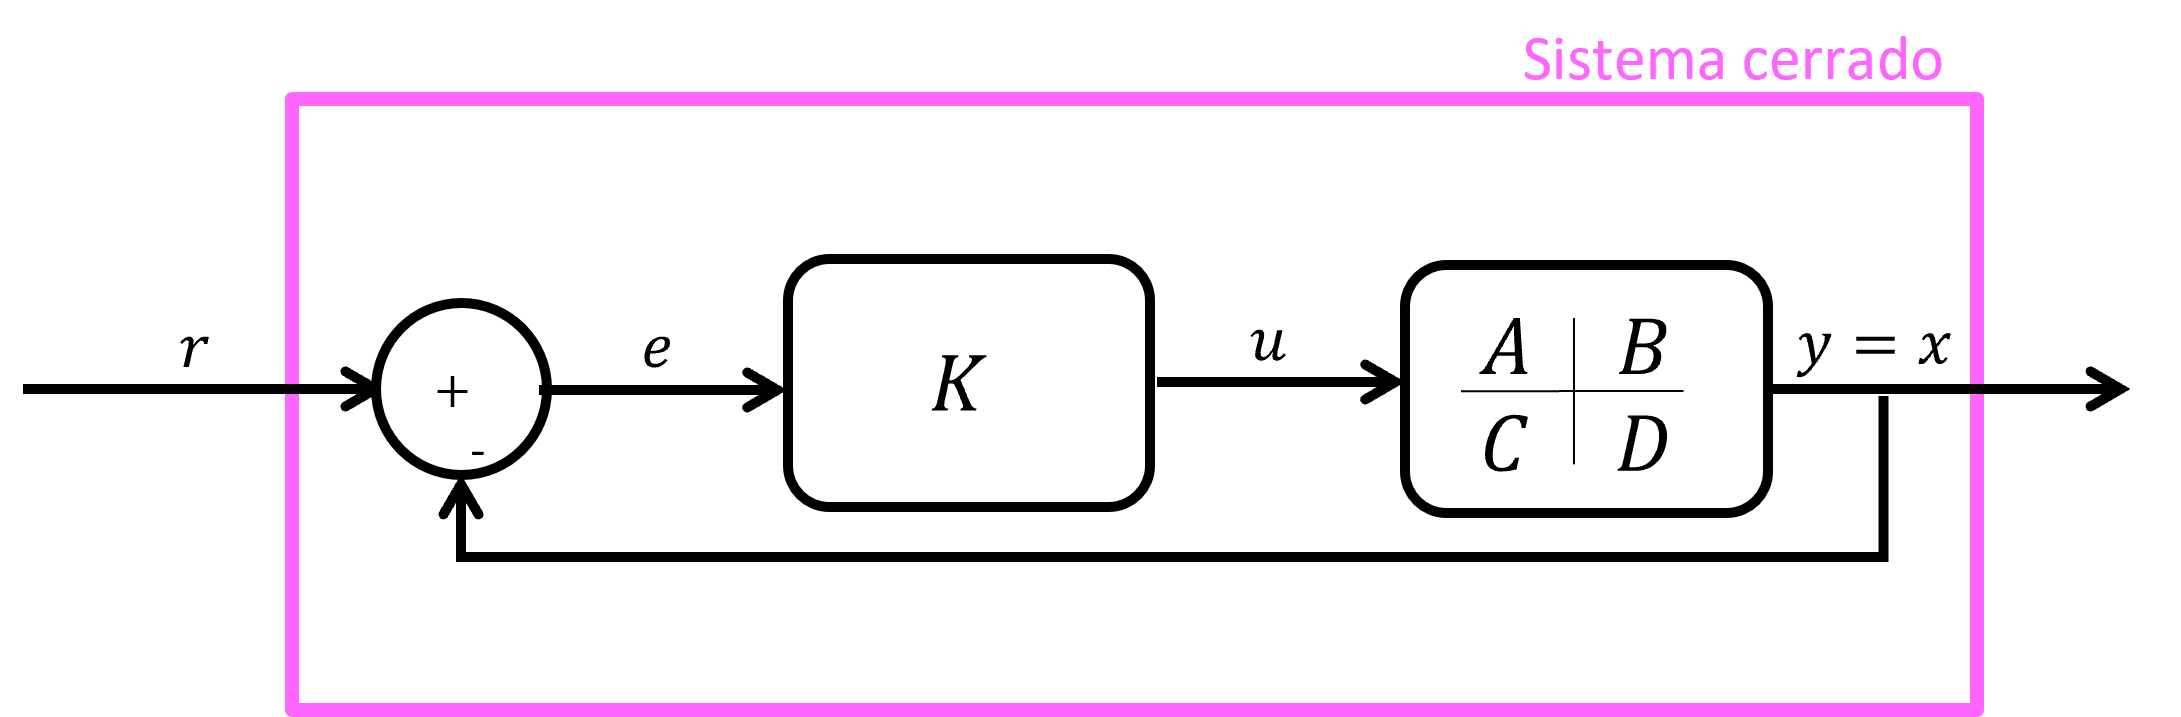
\includegraphics[scale=0.7]{Figuras/State_feedback.png}
\end{figure}
\underline{Objetivo}: Diseñar $K$ tal que $e=r-x\to 0$ para un tiempo $t_f$.\\
\par \underline{Definición}: El sistema de control ``full state feedback'' tiene relación con el hecho que el controlador cuenta con acceso a todos los estados del sistema.\\

\par Veamos la ecuación de estado del sistema:
\begin{align*}
    \dot{x}=Ax+Bu
\end{align*}
La señal de control:
\begin{align*}
    u=Ke
\end{align*}
La señal de error:
\begin{align*}
    e=r-x
\end{align*}

Luego:
\begin{align*}
    \dot{x} &= Ax+BK(r-x)\\
    \dot{x} &= (A-BK)x+BKr\\
\end{align*}
\begin{itemize}
    \item $A_{CL}=A-BK$: matriz de estado del sistema cerrado.
    \item $B_{CL}=BK$
\end{itemize}
\begin{align*}
    \dot{x}=A_{CL}x+B_{CL}r
\end{align*}
Para que el sistema cerrado sea \textcolor{red}{ESTABLE}, los valores propios de $A_{CL}$ deben tener partes reales estrictamente negativas:
\begin{align*}
    \text{Re}(eig(A_{CL}))<0
\end{align*}

\par Analicemos el diseño de un controlador utilizando una representación CCF:
\begin{align*}
\tenq{A}=\left[
    \begin{array}{cccc|c}
     -a_1 & -a_2 & \dots & -a_{n-1} & -a_n\\ \hline
     1 & & & 0 & 0\\
       & 1 & & & \vdots\\
       & & \ddots & & \\
     0 & & & 1 & 0  
    \end{array}\right]_{n\times n}
\end{align*}
\begin{align*}
\tenq{B}=\left[
    \begin{array}{c}
     1 \\ \hline
     0\\
    \vdots\\
     0  
    \end{array}\right]_{n\times 1}
\end{align*}
\begin{align*}
\tenq{K}=\left[
    \begin{array}{ccccc}
     k_{n-1} & k_{n-2} & \dots & k_1 & k_0
    \end{array}\right]_{1\times n}
\end{align*}

Calculemos $BK$:
\begin{align*}
\tenq{BK}=\left[
    \begin{array}{cccc|c}
     k_{n-1} & k_{n-2} & \dots & k_1 & k_0\\ \hline
      & & & & 0\\
      & & \tenq{0}_{(n-1)\times(n-1)} & & \vdots\\
      & & & & 0  
    \end{array}\right]_{n\times n}
\end{align*}

Ahora, calculemos $A_{CL}=A-BK$
\begin{align*}
\tenq{BK}=\left[
    \begin{array}{cccc|c}
     -(a_{n-1}+k_{n-1}) & -(a_{n-2}+k_{n-2}) & \dots & -(a_1+k_1) & -(a_0+k_0)\\ \hline
      & & & & 0\\
      & & \tenq{I}_{(n-1)\times(n-1)} & & \vdots\\
      & & & & 0  
    \end{array}\right]_{n\times n}
\end{align*}

Queremos encontrar los valores propios de $A_{CL}$. Escribamos la ecuación característica de $A_{CL}$
\begin{align*}
    \det(\tenq{A_{CL}}-\lambda \tenq{I})=0
\end{align*}

\begin{align*}
\tenq{BK}=\left[
    \begin{array}{cccc|c}
     -(\lambda+a_{n-1}+k_{n-1}) & -(a_{n-2}+k_{n-2}) & \dots & -(a_1+k_1) & -(a_0+k_0)\\ \hline
      1 & -\lambda & & & 0\\
      & 1 & -\lambda & & \vdots\\
      & & \ddots & \ddots & 0\\
      & & & 1 & -\lambda\\
    \end{array}\right]=0
\end{align*}

La ecuación característica resulta ser:
\begin{align*}
    \lambda^n+(a_{n-1}+k_{n-1})\lambda^{n-1}+(a_{n-2}+k_{n-2})\lambda^{n-2}+...+(a_{1}+k_{1})\lambda+(a_{0}+k_{0})=0
\end{align*}
Si queremos ubicar los polos en una posición particular, o sea, queremos fijar los polos de la siguiente manera:
$$ \lambda=\{p_1,p_2,p_3,..,p_n \}$$

Podemos reescribir la ecuación característica de la siguiente forma:
$$(\lambda-p_1)(\lambda-p_2)(\lambda-p_3)...(\lambda-p_n)=0 $$

Desarrollando el polinomio:
$$\Longrightarrow \lambda^n+\alpha_{n-1}\lambda^{n-1}+...+\alpha_1\lambda+\alpha_0=0 $$
Entonces, el controlador $K$ se define como:
\begin{align*}
    \alpha_{n-1} = a_{n-1}+k_{n-1} &\Longrightarrow k_{n-1} = \alpha_{n-1}-a_{n-1}\\
    \alpha_{n-2} = a_{n-2}+k_{n-2} &\Longrightarrow k_{n-2} = \alpha_{n-2}-a_{n-2}\\
    \vdots \\
    \alpha_0 = a_0+k_0 &\Longrightarrow k_0 = \alpha_0-a_0\\
\end{align*}
Donde $\alpha_i$ se obtiene de la posición deseada de los polos. \\
\par Entonces, si el sistema es CCF, podemos diseñar $K$ al elegir la posición de los polos de manera apropiada $\Longrightarrow$ \textcolor{red}{POLE PLACEMENT}\\
\par \underline{Nota}: Si el sistema no es CCF, entonces se puede transformar a CCF utilizando matriz de transformación $\tenq{T}$, provisto que el sistema sea controlable.\\
\par Sea la realización:
\begin{align*}
    \tend{x}=Ax+Bu \xrightarrow[]{x=Tz} \dot{z}=A_cz+B_cu
\end{align*}
Sea $T \in \mathbb{R}^{n\times n}$, tal que $T^{-1}$ existe
\begin{align*}
    \Longrightarrow x&=Tz\\
    \Longrightarrow \dot{x}&=T\dot{z}
\end{align*}
Reemplazando:
\begin{align*}
    T\dot{z} &= ATz+Bu\\
    \Longrightarrow \dot{z}&=T^{-1}ATz+T^{-1}Bu\\
    \dot{z} &= A_cz+B_cu
\end{align*}

``Pole placement'', pasos a seguir:
\begin{enumerate}
    \item Buscar $T$ y transformar a CCF ($A_c$ y $B_c$).
    \item Encontrar $K_c$ , en base a la ubicación de polos deseados.
    \item Volver al sistema original (asuma $r=0$)
\end{enumerate}
\begin{align*}
    \Longrightarrow \dot{z} &= (A_c-B_cK_c)z\\
    \Longrightarrow T\dot{z} &= TA_cz+TB_cz\\
    \Longrightarrow \dot{x} &= TT^{-1}ATz-TT^{-1}BK_cz\\
    \Longrightarrow \dot{x} &= Ax-BK_cT^{-1}x\\
    \Longrightarrow \dot{x} &= (A-BK)x
\end{align*}
donde  $K=K_cT^{-1}$, controlador para el sistema original.



%----------- Cap3 -----------%
\chapter{Teoría de Sistemas Lineales}



\section{Matriz de transición de Estados}
Sea un sistema LTI autónomo (es decir, sin entrada u)
\begin{align*}
    \tend{\dot{x}}(t)=\tenq{A}\tend{x}(t), \quad \tend{x}(0)=\tend{x_0}
\end{align*}
La solución $\tend{x}(t)$ se puede obtener utilizando transformación de Laplace:\\
\par \underline{Definición}: $\mathcal{L}\{\tend{x}(t)\}=\tend{X}(s)$\\
\par \underline{Definición}: $\mathcal{L}\{\tend{\dot{x}}(t)\}=s\tend{X}(s)-\tend{x_0}$\\
\par Reemplazando:
\begin{align*}
    \Longrightarrow s\tend{X}-\tend{x_0} &= \tenq{A}\tend{X}\\
    \Longrightarrow (s\tenq{I}-\tenq{A})\tend{X} &=\tend{x_0}\\
    \Longrightarrow \tend{X}(s) &= (s\tenq{I}-\tenq{A})^{-1}\tend{x_0}\\
    \Longrightarrow \tend{x}(t) &= e^{\tenq{A}t}\tend{x_0}\\
    \Longrightarrow \tend{x}(t) &= \tenq{\phi}(t)\tend{x_0}
\end{align*}
Donde $\tenq{\phi}(t)=e^{\tenq{A}t}$ es la \textcolor{red}{matriz de transición de estados del sistema}. \\
\par \underline{Aparte}: Expansión e series de Taylor.\\
Sea f(t) es continua y suave, entonces la expansión de Taylor respecto a $t=\alpha$
$$f(t)=f(\alpha)+\frac{\dot{f}(\alpha)}{1!}(t-\alpha)+\frac{\ddot{f}(\alpha)}{2!}(t-\alpha)^2+... $$
Podemos utilizar esto para escribir una expansión de la función escalar $f(t)=e^{at}$, para $\alpha=0$.
$$e^{at}=1+at+\frac{1}{2!}a^2t^2+\frac{1}{3!}a^3t^3+... $$

\par Se puede demostrar que la expansión de Taylor de $\tenq{\phi}(t)$:
\begin{align*}
    \tenq{\phi}(t)=e^{\tenq{A}t}=\tenq{I}+\tenq{A}t+\frac{1}{2!}\tenq{A}^2t^2+\frac{1}{3!}\tenq{A}^3t^3+...
\end{align*}

\underline{Nota}: $\tenq{\phi}(t)$ satisface la ecuación de estado:
\begin{align*}
    \Longrightarrow \tend{x}(t) &= \tenq{\phi}(t)\tend{x_0}\\
    &= \left[\tenq{I}+\tenq{A}t+\frac{1}{2!}\tenq{A}^2t^2+...\right]\tend{x_0}\\
    \Longrightarrow \tend{\dot{x}}(t) &= \left[\tenq{A}+\frac{2}{2!}\tenq{A}^2t+...\right]\tend{x_0}\\
    &= \tenq{A}\left[\tenq{I}+\tenq{A}t+\frac{1}{2!}\tenq{A}^2t^2+...\right]\tend{x_0}\\
    \Longrightarrow \tend{\dot{x}}(t) &= \tenq{A}\tenq{\phi}(t)\tend{x_0}=\tenq{A}\tend{x_t} \quad \text{Ecuación de Estado}
\end{align*}

Si tenemos un sistema LTI no autónomo:
\begin{align*}
    \tend{\dot{x}}(t) &= \tenq{A}\tend{x}(t)+\tenq{B}\tend{u}(t)\\
    \Longrightarrow s\tend{X}-\tend{x_0} &= \tenq{A}\tend{X}+\tenq{B}\tend{U}\\
    \Longrightarrow (s\tenq{I}-\tenq{A})\tend{X} &= \tend{x_0}+\tenq{B}\tend{U}\\
    \Longrightarrow \tend{X}(s) &= (s\tenq{I}-\tenq{A})^{-1} \tend{x_0}+(s\tenq{I}-\tenq{A})^{-1} \tenq{B}]tend{U}(s)\\
    \Longrightarrow \tend{x}(t) &= \tenq{\phi}(t)\tend{x_0}+\left[ \tenq{\phi}(t)\tenq{B} \right] \ast u(t)\\
    \tend{x}(t) &= \tenq{\phi}(t)\tend{x_0}+\int_0^t\tenq{\phi}(t-\tau)\tenq{B}\tend{U}(\tau)d\tau
\end{align*}

Solución $\tend{x}(t)$ del sistema LTI no-autónomo.\\
\par Sobre las propiedades de $\tenq{A}$, del problema de valores propios:
$$\tenq{A}\tend{v}=\lambda\tend{v}$$
donde $\tend{v}$ y $\lambda$ son el vector y valor propio asociado.
\begin{align*}
    \Longrightarrow \tenq{\phi}(t)\tend{v} &= \left[\tenq{I}+\tenq{A}t+\frac{1}{2!}\tenq{A}^2t^2+...\right]\tend{v}\\
    &= \tend{v}+\tenq{A}\tend{v}t+\frac{1}{2!}\tenq{A}^2\tend{v}t^2+... \\
    &= \tend{v}+\lambda\tend{v}t+\frac{1}{2!}\lambda^2\tend{v}t^2+... \\
    &= \left[ 1+\lambda t+\frac{\lambda^2}{2!}+\frac{\lambda^3}{3!}t^3\right]\tend{v}
\end{align*}
Si $\tend{x_0}=\tend{v}$, entonces $\tend{x}(t)=\tenq{\phi}(t)\tend{v}$\\
\par Pregunta: ¿Es $\phi(t)$ una serie infinita?\\
$$\lim_{t \to \infty} \phi(t)<\infty $$ sí y solo si $\text{Re}(\lambda)<0$. 
Entonces el sistema LTI es estable!\\

\par \underline{Definición}: Una matriz $\tenq{A}$ se dice que es \textcolor{red}{Hurwitz} ssi los valores propios de $\tenq{A}$ tienen una parte real estrictamente negativa.


\section{Plano de Fase}
Representación gráfica de las trayectorias de un sistema dinámico autónomo en el plano.
\begin{figure}[H]
\centering
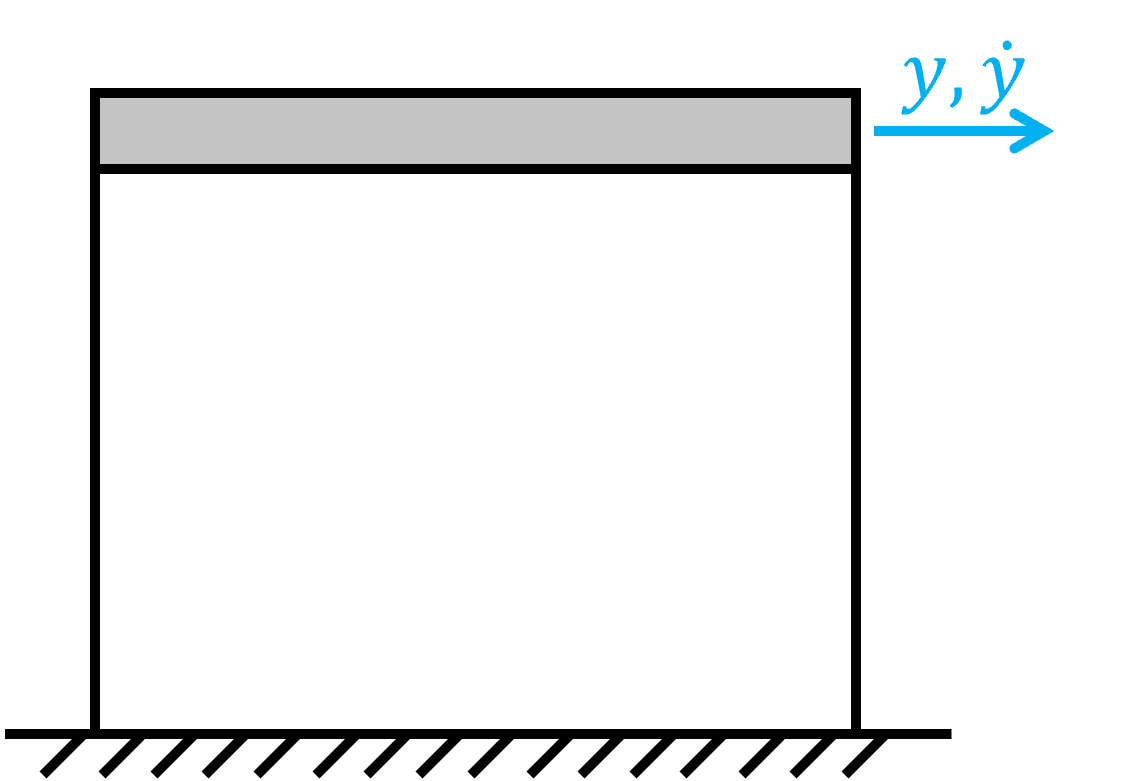
\includegraphics[scale=0.7]{Figuras/leccion11.png}
\end{figure}
\begin{align*}
    \Longrightarrow \tend{\dot{x}}(t) =\tend{f}(\tend{x},t)=\tenq{A}\tend{x}(t)
\end{align*}
donde 
$\tend{x}=\begin{bmatrix}\tend{y}\\ \tend{\dot{y}}\end{bmatrix}$, con condiciones iniciales $y_0$, $\dot{y}_0$.
\begin{figure}[H]
\centering
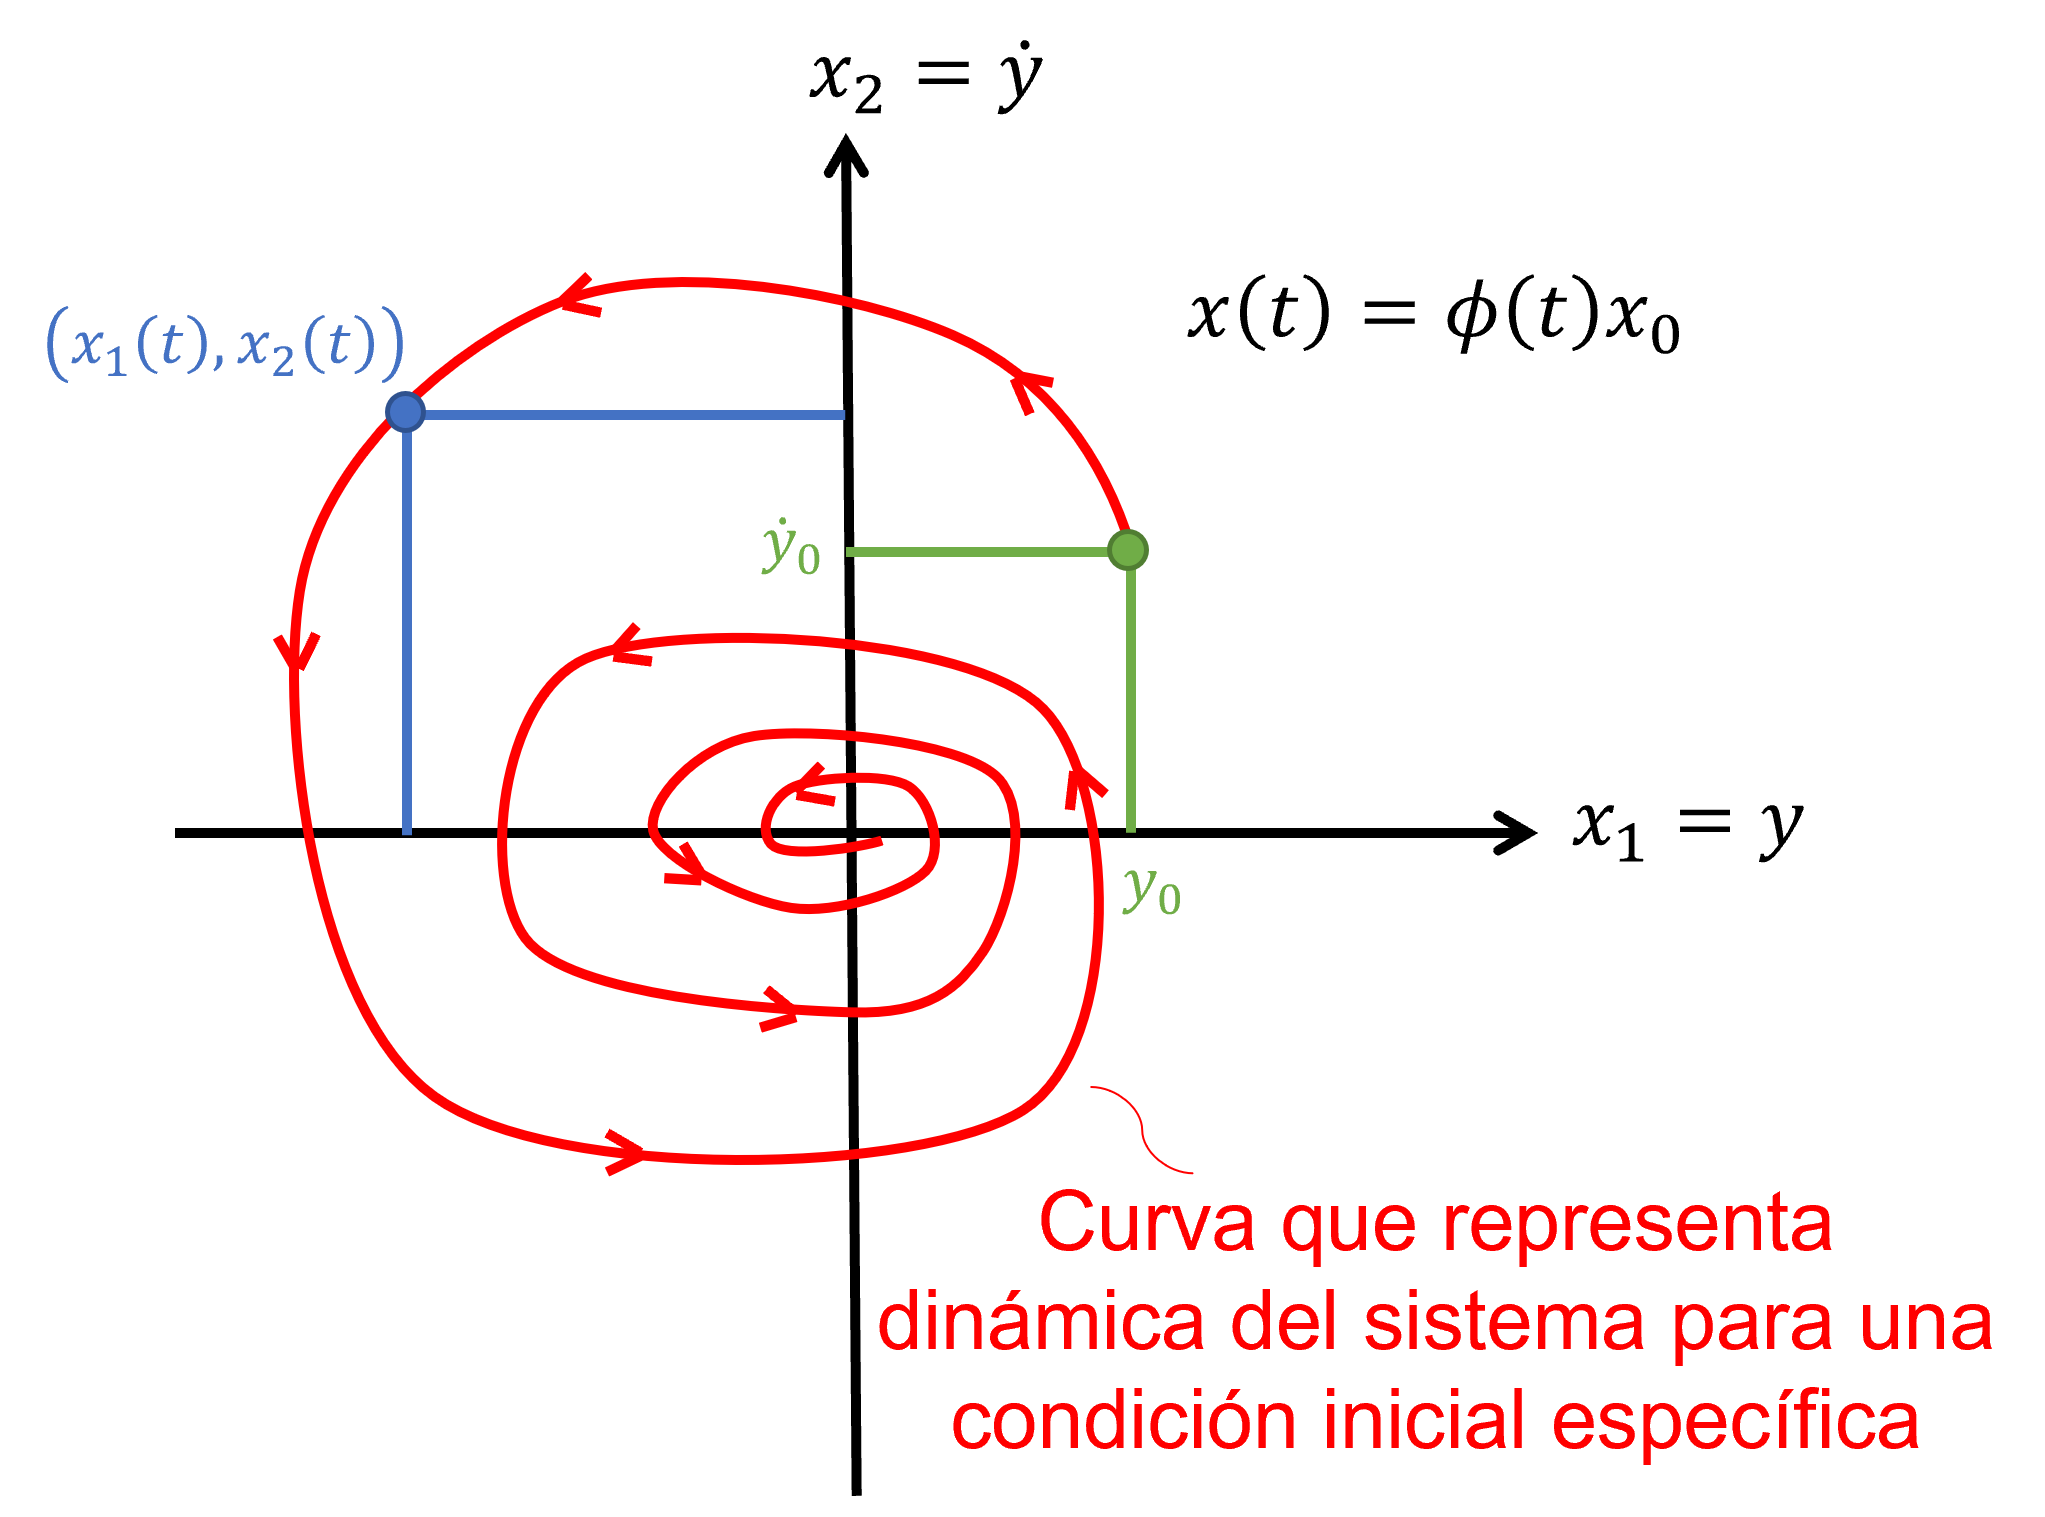
\includegraphics[scale=0.7]{Figuras/plano_de_fase.png}
\end{figure}
\begin{figure}[H]
\centering
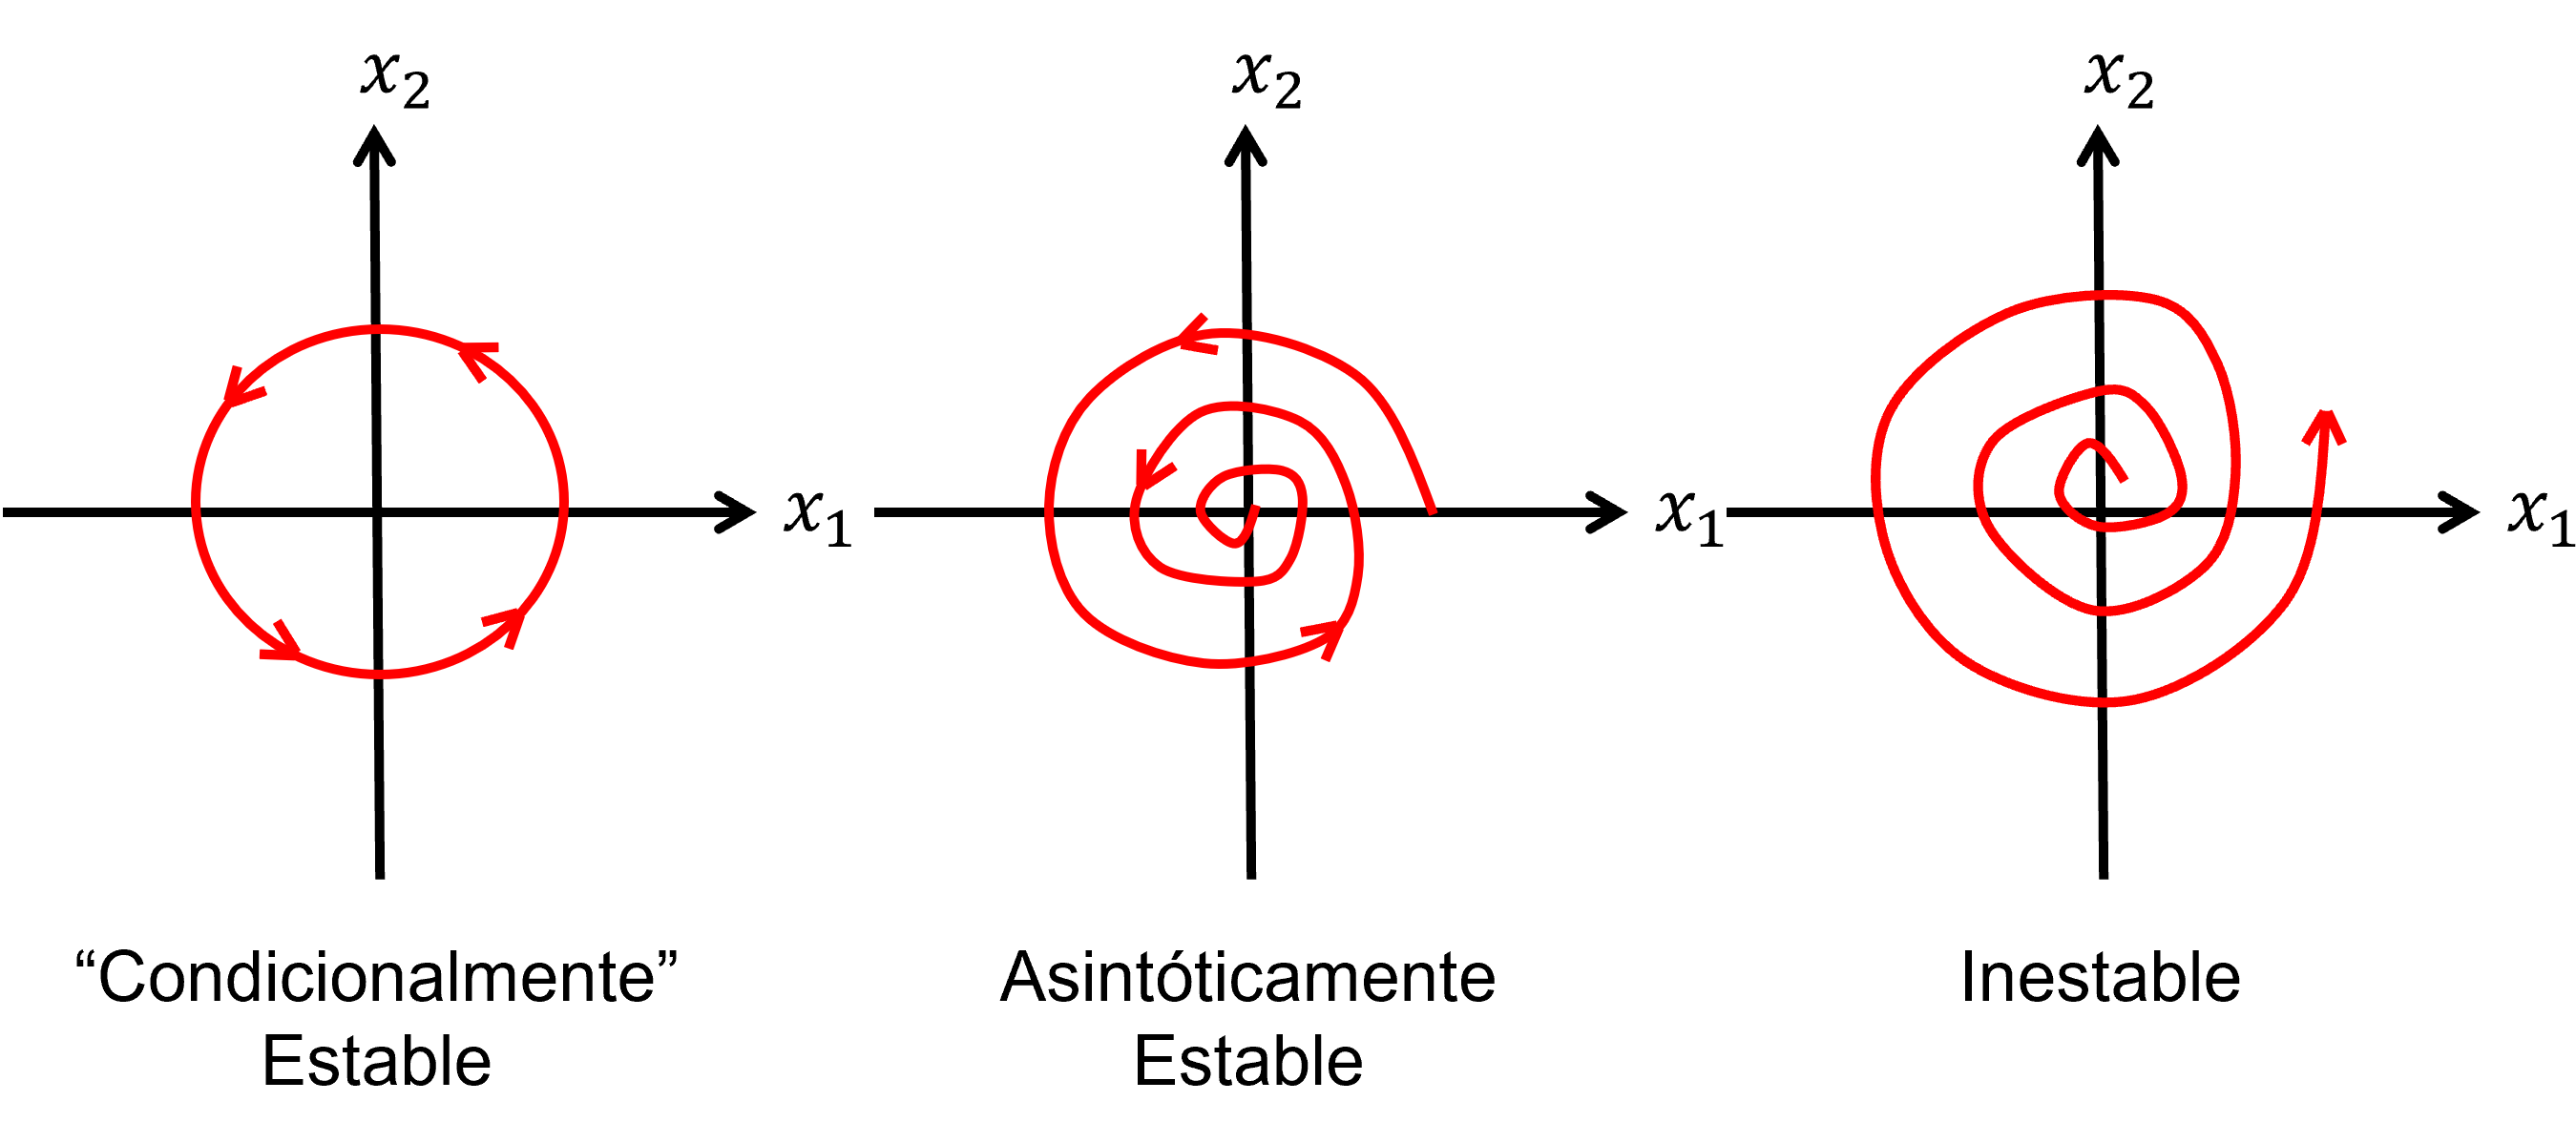
\includegraphics[scale=0.7]{Figuras/plano_de_fase.png_2.png}
\end{figure}

\section{Equilibrio}
Sea el sistema dinámico LTI:
$$\tend{\dot{x}}=\tenq{A}\tend{x}+\tenq{B}\tend{u} $$

\underline{Definición}: El equilibrio del sistema está dado por:
$$ \tend{\dot{x}}=\tend{0} \Longrightarrow \tend{x} \text{ no cambia con el tiempo}$$
Entonces:
\begin{align*}
    \Longrightarrow \tend{0}=\tenq{A}]\tend{x_e}+\tenq{B}\tend{u_e} \\
\end{align*}
donde $\tend{x_e}$ s el vector de estado en equilibrio y $\tend{u_e}$ es el vector de entrada en el equilibrio = constante.
\begin{align*}
    \Longrightarrow \tend{x_e}=-\tenq{A}^{-1}\tenq{B}\tend{u_e} \Longrightarrow \text{ Equilibrio Estático}
\end{align*}
Si $\tend{u_e}=\tend{0}\Longrightarrow\tend{x_e}=\tend{0}$.\\
\par \underline{Nota}: Sistemas lineales presentan sólo un punto de equilibrio $\tend{x_e}$.  




\section{Estabilidad de Lyapunov}
Sea un sistema dinámico LTI y autónomo: $\dot{x}=Ax$, $x(0)=x_0$.\\
\par Sea $x_e$ el punto de equilibrio del sistema. Sin pérdida de generalidad, podemos asumir que $x_e=0$.\\
\par Vamos a definir la estabilidad respecto a un punto de equilibrio.\\
\par \underline{Definición}: $x_e$ es estable en el sentido de Lyapunov si para cualquier $\varepsilon >0$ existe un $\delta >0$ tal que:
$$||x_0-x_e||<\delta\Longrightarrow ||x(t)-x_e||<\varepsilon, \quad \forall t>0$$
\begin{figure}[H]
\centering
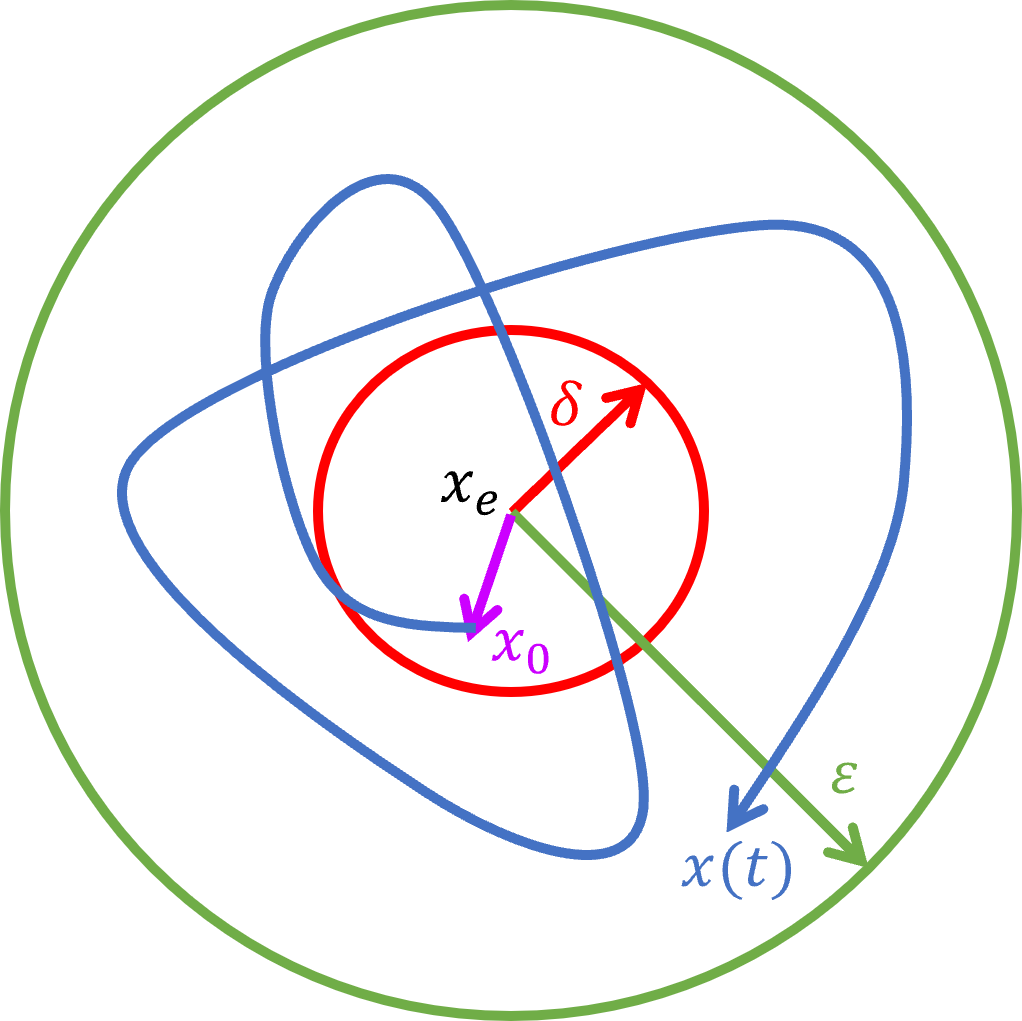
\includegraphics[scale=0.7]{Figuras/Lyapunov.png}
\end{figure}
* Mínima restricción que podemos imponer para satisfacer estabilidad.

\subsection{Definición Estabilidad Asintótica}
$x_e$ es asintóticamente estable si existe $\delta>0$ tal que:
\begin{itemize}
    \item $||x_0-x_e||<\delta$
    \item $x_e$ es estable en el sentido de Lyapunov
    \item $\lim_{t\to\infty}x(t)=x_e$
\end{itemize}
\begin{figure}[H]
\centering
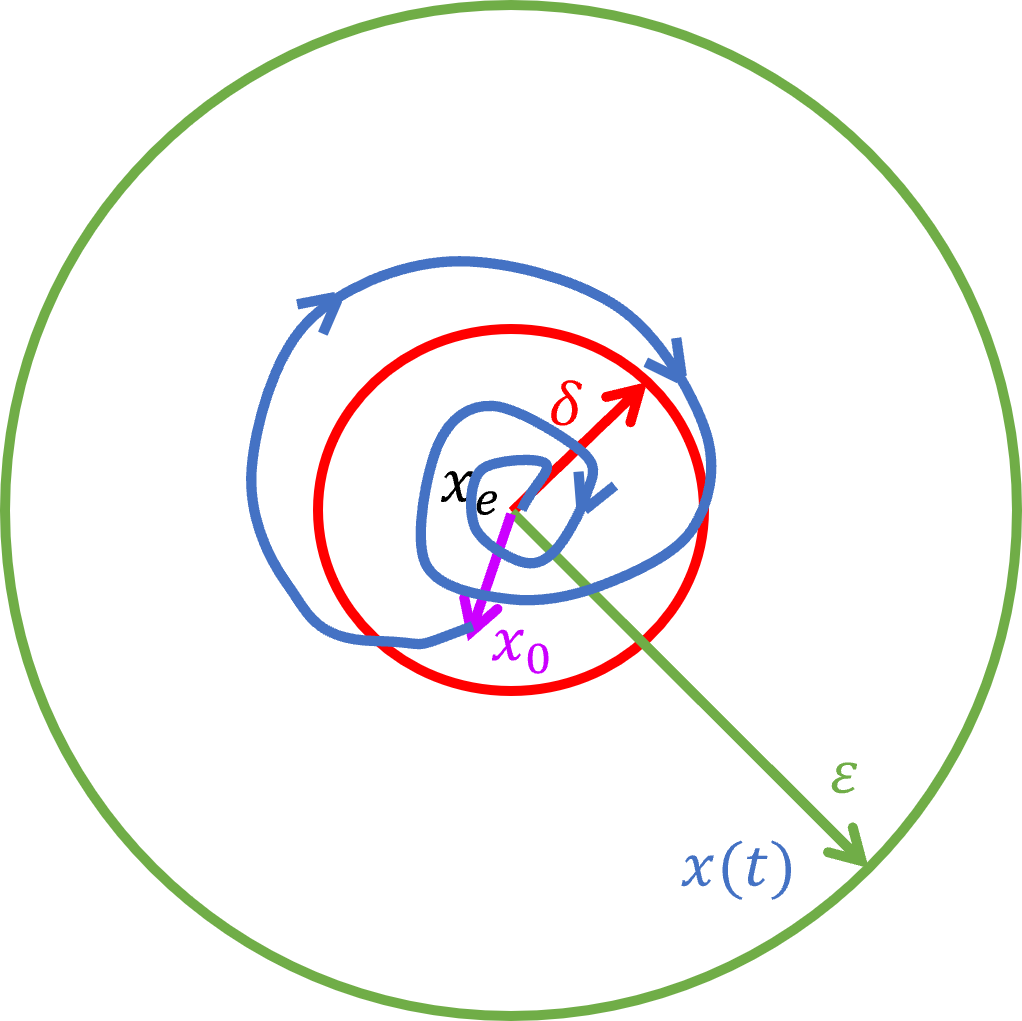
\includegraphics[scale=0.7]{Figuras/asintotica.png}
\end{figure}

\subsection{Definición Estabilidad Asintótica Global}
$x_e$ es estable asintótica global ssi es asintóticamente estable para $\delta \to \infty$.

\begin{table}[H]
    \centering
    \begin{tabular}{c|c|c|c|}
                & \raisebox{-\totalheight}{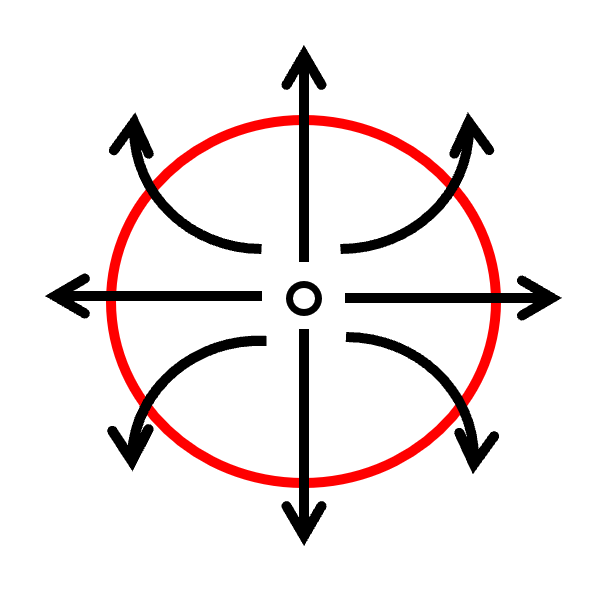
\includegraphics[scale=0.5]{Figuras/global1.png}} & \raisebox{-\totalheight}{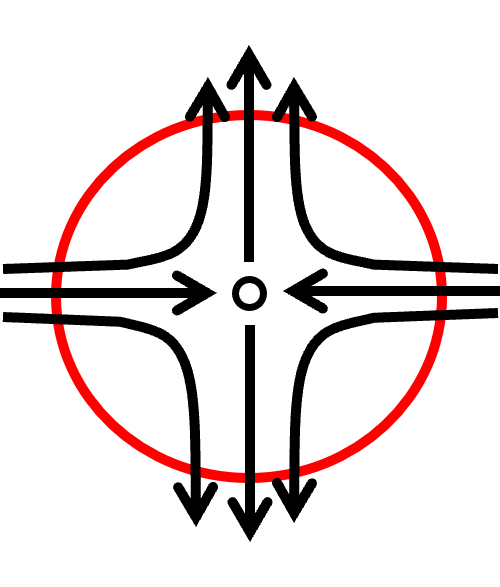
\includegraphics[scale=0.5]{Figuras/global2.png}} & \raisebox{-\totalheight}{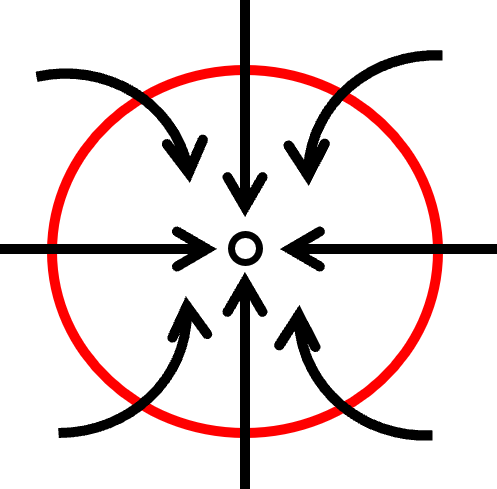
\includegraphics[scale=0.5]{Figuras/global3.png}}\\ \hline
         Estable & \xmark & \xmark & \cmark\\
         Asint. Est. & \xmark & \xmark &\cmark \\
         Goblal Asint. Est. & \xmark & \xmark & \textbf{???}
    \end{tabular}
\end{table}


\section{Límites de Estabilidad para sistemas LTI}
Sea $\dot{x}=Ax$, $x(t)\in \mathbb{R}^n$, $x(0)=x_0$.\\
Solución: $x(t)=\phi(t)x_0$, donde $\phi(t)=e^{At}$.\\
\par Suponiendo que $\phi(t)$ es finita,
$$||\phi(t)||=||e^{At}||\leq\beta<\infty $$
Luego:
\begin{align*}
    x(t)-x_e &= \phi(t)x_0-x_e\\
    &= \phi(t)x_0-\phi(t)x_e\\
    &= \phi(t)[x_0-x_e]
\end{align*}
\underline{Nota}: Si $x_0=x_e$, entonces $x(t)=x_e$ para $\phi(t)x_e=x_e$.\\
\par Entonces:
\begin{align*}
    ||x(t)-x_e||=||\phi(t)[x_0-x_e]||\leq||\phi(t)||\cdot||x_0-x_e||
\end{align*}
Si $||x_0-x_e||<\delta$ y $||x(t)-x_e||\leq \beta||x_0-x_e||$.\\
\par Sea $\varepsilon$, tal que $\delta=\varepsilon/\beta$.
$$\Longrightarrow ||x(t)-x_e||<\varepsilon $$
Por lo tanto, si $\phi(t)$ es finito, implica que $x_e$ es estable en el sentido de Lyapunov.\\
\par $\phi(t)$ es finito si y solo si $A$ es Hurwitz:
\begin{align*}
    \text{Re}\left(\text{eig}(A)\right)<0\Longrightarrow \text{Estabilidad}
\end{align*}

\section{Función Candidata de Lyapunov}
\underline{Definición}: Sea una función $V(x)$, $\mathbb{R}^n\to \mathbb{R}$, tal que: 
\begin{itemize}
    \item $V(x_e)=0$
    \item $V(x)>0$, $\forall x\neq x_e$ ($V$ es una función definida positiva)
    \item $V$ y su primera derivada son finitas
\end{itemize}
Entonces, $V$ es una función candidata de Lyapunov.\\
\par \underline{Teorema}: Si $V(x)$ s una función candidata de Lyapunov para $x_e$ en una región $\Omega$ vecina a $x_e$:
\begin{itemize}
    \item[a)] $x_e$ es estable en el sentido de Lyapunov si:
    $$\frac{dV}{dt}\leq 0, ~\forall x\in \Omega $$
    \item[b)] $x_e$ es asintóticamente estable si:
    $$\frac{dV}{dt}< 0, ~\forall x\in \Omega$$
    \item[c)] $x_e$ es global asintóticamente estable si:
    $$\frac{dV}{dt}< 0, ~\forall x\in \Omega$$
    donde $\Omega \in \mathbb{R}^n$ y $V$ no tiene límite radial.
\end{itemize}

\underline{Ilustración}: Sea $x=\begin{bmatrix}x_1\\ x_2\end{bmatrix}$, $x\in \mathbb{R}^2$, $x_e=0$.\\
Sea $V(x)=x^\top x$ es una función candidata de Lyapunov.

\begin{figure}[H]
\centering
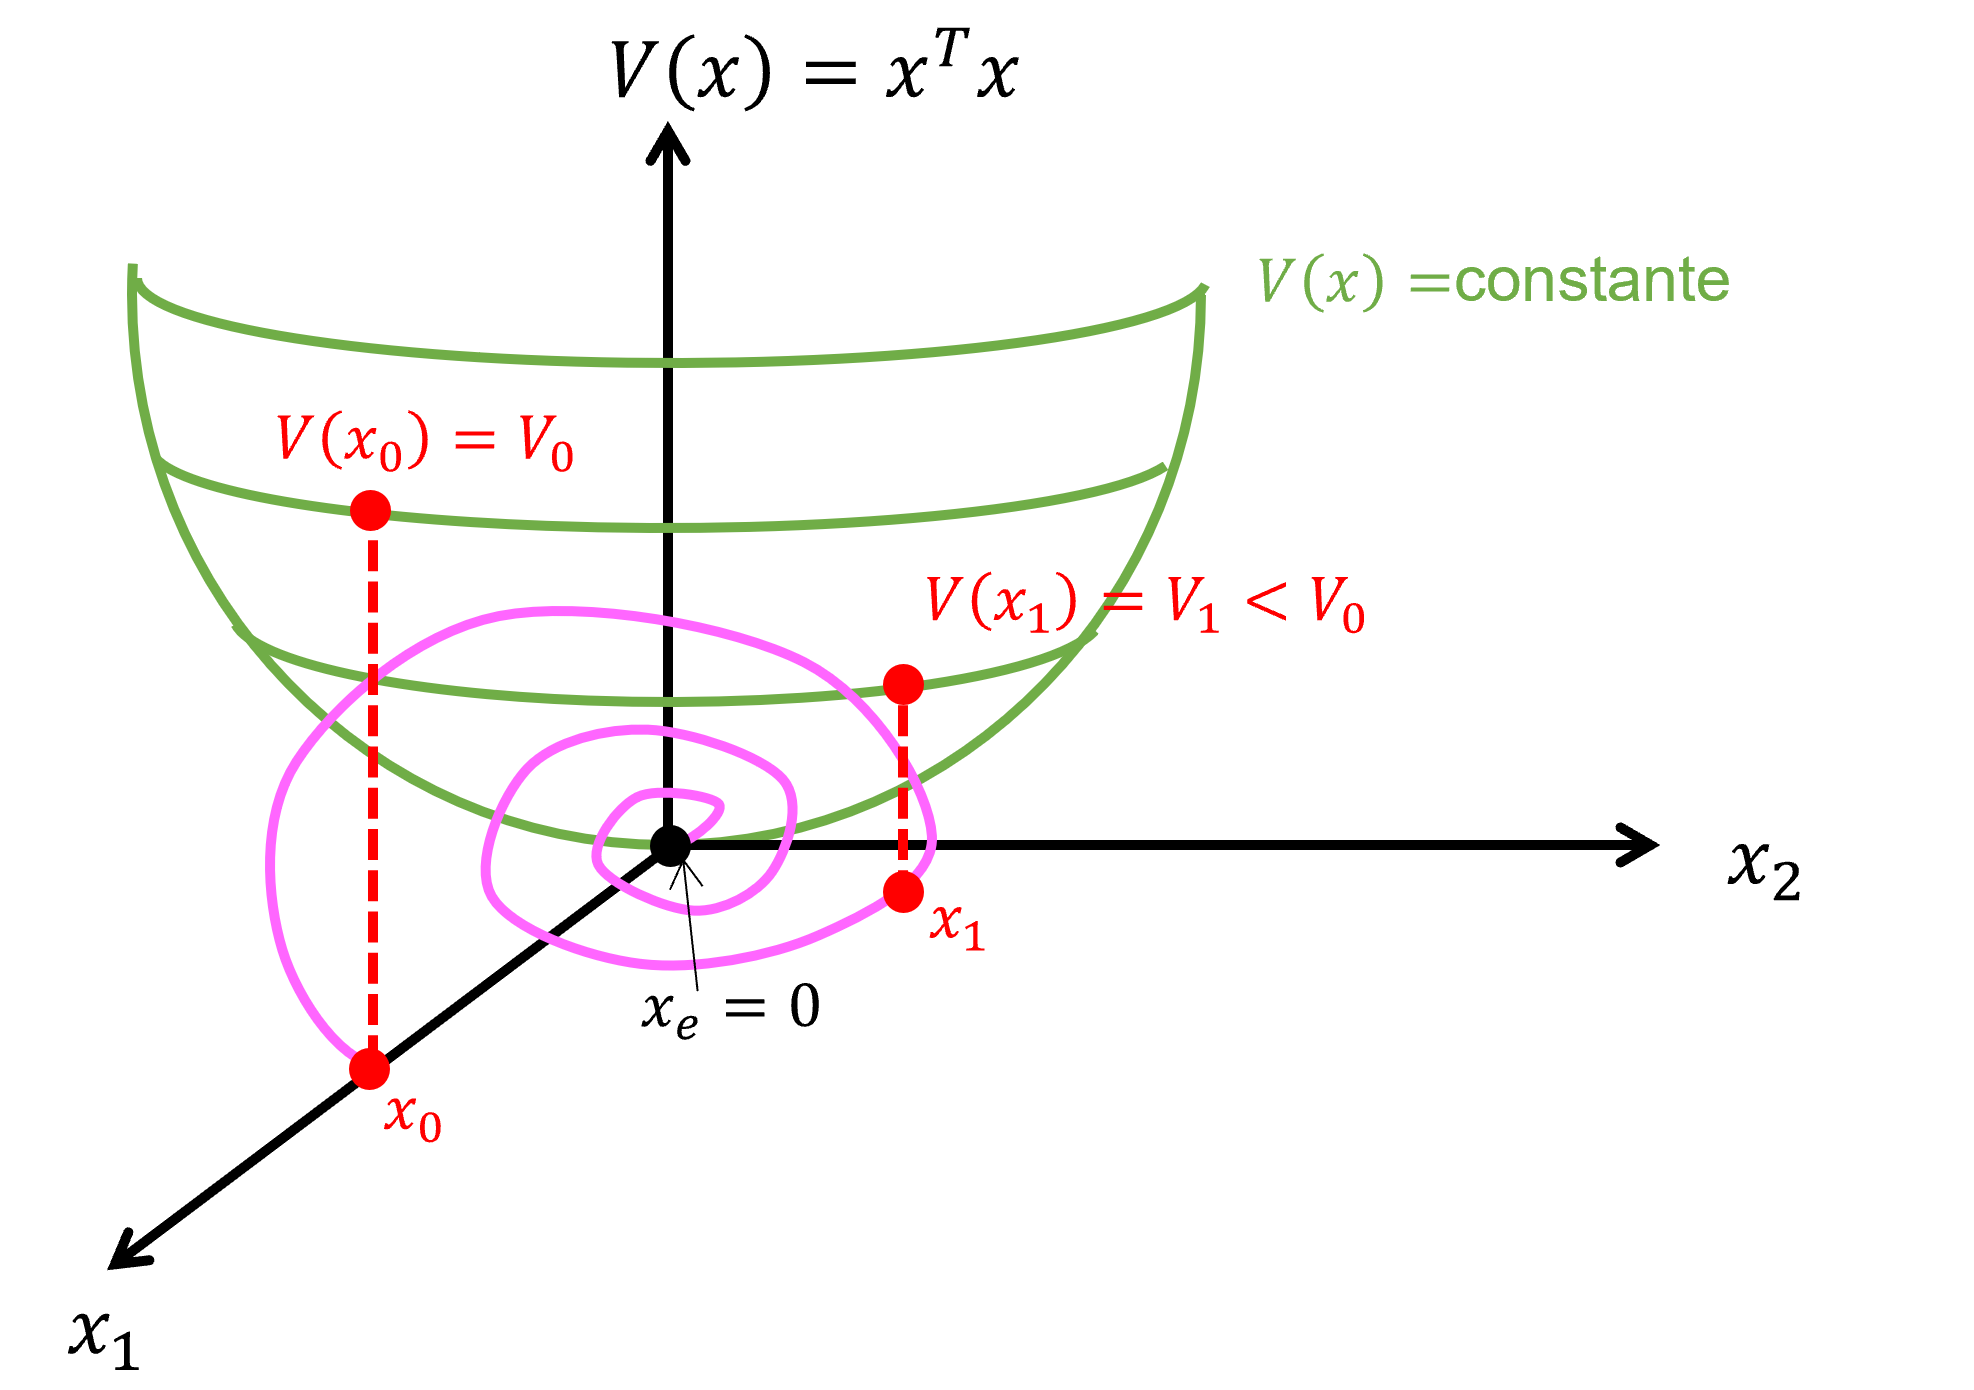
\includegraphics[scale=0.7]{Figuras/ilu_lyapunov.png}
\end{figure}



$$\frac{dV}{dt}<0 \Longrightarrow V(x) \quad V(x) \text{ decrece cuando t aumenta}$$

Notar que $V=V(x(t))$. Entonces:
\begin{align*}
    \frac{dV}{dt} &= \frac{\partial V}{\partial x}\cdot \frac{\partial x}{\partial t}  \quad \text{Regla de la cadena}\\
    &= \sum_{i=1}^n \frac{\partial V}{\partial x_i}\cdot\frac{\partial x_i}{\partial t}\\
    &= \begin{bmatrix}\frac{\partial V}{\partial x_1} &...& \frac{\partial V}{\partial x_n}\end{bmatrix}\begin{bmatrix}\dot{x}_1\\ \vdots \\ \dot{x}_n\end{bmatrix}\\
    &= \nabla V\cdot \dot{x}
\end{align*}

\begin{align*}
    \frac{dV}{dt}=\nabla V\cdot \dot{x}<0, ~\forall t
\end{align*}

\underline{Ilustración}: Dibujemos una línea de contorno de $V(x)$: \\
\begin{figure}[H]
\centering
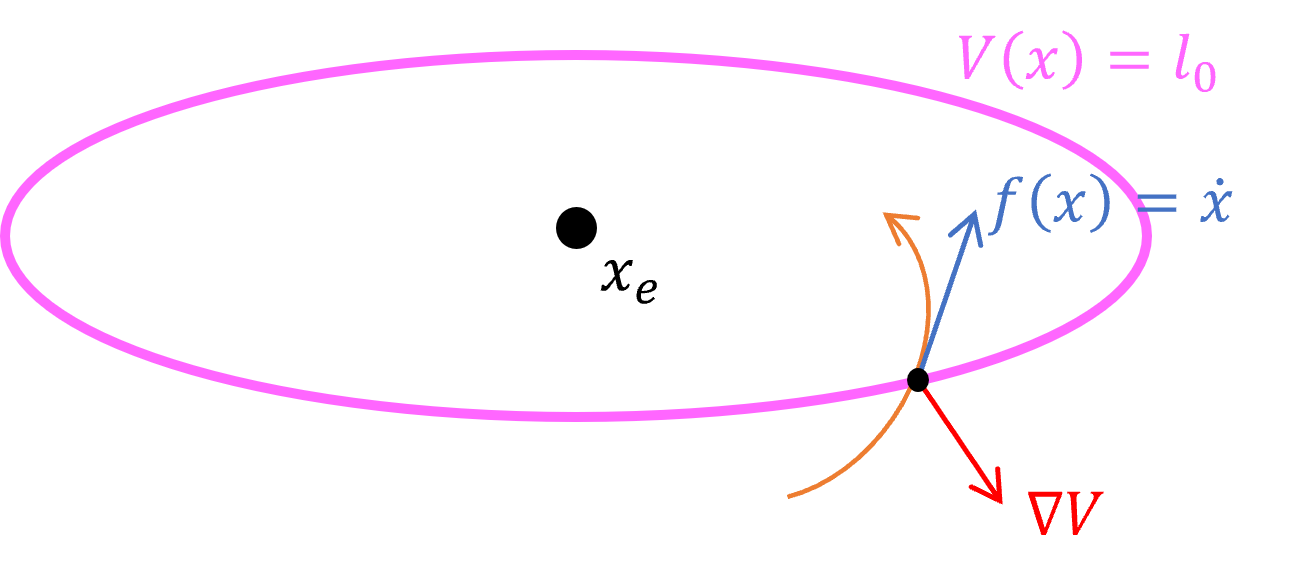
\includegraphics[scale=0.7]{Figuras/ilu_lyapunov2.png}
\end{figure}
$\nabla V\cdot f(x)<0 \Longrightarrow$ Entonces el sistema se acerca a $x_e$.\\
$\Longrightarrow x_e$ es un punto de atracción ``sumidero''.\\

\par Para $\dot{x}=Ax$, y sea $V(s)=x^\top Px$, donde $P$ es una matriz definida positiva y simétrica.
$$\frac{dV}{dt}=\nabla V\cdot \dot{x}<0 $$ para un sistema asintóticamente estable.\\
\begin{align*}
    \nabla V=\frac{\partial}{\partial \tend{x}} (\tend{x}^\top \tenq{P}\tend{x})=2\tenq{P}\tend{x} \quad \text{Por demostrar}
\end{align*}
Entonces:
\begin{align*}
    \frac{dV}{dt} &= (2Px)^\top (Ax)= (2x^\top P^\top)(Ax)\\
    &= (x^\top P^\top)(Ax)+x^\top P^\top Ax\\
    &= (Px)^\top(Ax)+x^\top PAx\\
    &= (Ax)^\top(Px)+x^\top PAx\\
    &= x^\top A^\top Px+x^\top PAx\\
    &= x^\top (A^\top P+PA)x<0
\end{align*}

Por lo tanto, $A^\top P+PA\prec 0$ definida negativa para que el sistema sea asintóticamente estable.\\
\par Sea $Q$ una matriz definida positiva y simétrica, tal que:
\begin{align*}
    A^\top P+PA &= -Q\\
    A^\top P+PA+Q &= \emptyset \quad \text{Ecuación de Lyapunov}
\end{align*}

\underline{Teorema}: Dado $Q \succ 0$, existe un $P\succ 0$ simétrica que satisface:
$$A^\top P+PA+Q=\emptyset $$
entonces, $\dot{x}=Ax$ es asintóticamente estable.



\section{Teorema de Cayley-Hamilton}
\underline{Teorema}: Sea una matriz $A\in\mathbb{R}^{n\times n}$, cuya ecuación característica está dada por el siguiente polinomio de orden n:
\begin{align*}
    \Delta (A)=\text{det}(sI-A)=s^n+\alpha_{n-1}s^{n-1}+...+\alpha_1s+\alpha_0=0
\end{align*}
donde $\alpha_i\in\mathbb{R}$, $i\in [0,n-1]$, son los coeficientes del polinomio característico de $A$. \\
\par Entonces, la matriz $A$ también satisface la ecuación característica:
\begin{align*}
    \Delta (\tenq{A})=\tenq{A}^n+\alpha_{n-1}\tenq{A}^{n-1}+...+\alpha_1\tenq{A}+\alpha_0\tenq{I}=\tenq{0}
\end{align*}

Del teorema, podemos despejar $\tenq{A}^n$:
\begin{align*}
    \tenq{A}^n &= -\left[\tenq{A}^n+\alpha_{n-1}\tenq{A}^{n-1}+...+\alpha_1\tenq{A}+\alpha_0\tenq{I} \right]
\end{align*}

El poder de una matriz se escribe como una serie polinomial de orden igual al exponente del poder.\\
\par $\Longrightarrow$ Este resultado es útil para evaluar la matriz de transición $\phi(t)$
\begin{align*}
    \phi(t)=e^{At}=\sum_{i=0}^\infty \beta_i(t)A^i \overset{\text{(C-H)}}{=} \sum_{i=0}^{n-1}\gamma_i(t)A^i
\end{align*}
\underline{Nota}: Este resultado es útil para evaluar $\phi(t)$ como una serie finita en términos de $A^i$.

\section{Controlabilidad}
La controlabilidad es una propiedad d cualquier sistema dinámico.\\
\par $\Longrightarrow$ Sea el sistema LTI: $\dot{x}=Ax+Bu$, $x\in \mathbb{R}^n$, $u\in\mathbb{R}^p$. Buscamos $u(t)$ tal que los estados vayan de $x(t)$ a cero en un tiempo finito $t_1$. \\
\par \underline{Solución}: $x(t)=\phi(t)x_0+\int_0^t \phi(t-\tau)Bu(\tau)d\tau$
\begin{align*}
    x(t_1)=0=\phi(t_1)x_0+\int_0^{t_1} \phi(t_1-\tau)Bu(\tau)d\tau
\end{align*}

\underline{Aparte}: $\phi(t_1-\tau)=e^({A(t_1-\tau)}=e^A\cdot e^{-A\tau}=\phi(t_1)\phi(-\tau)$

\begin{align*}
    \Longrightarrow 0 &=\phi(t_1)\left[x_0+\int_0^{t_1}\phi(-\tau)Bu(\tau)d\tau\right] \\
    -x_0 &= \int_0^{t_1}\phi(-\tau)Bu(\tau)d\tau
\end{align*}

Por el teorema de Cayley-Hamilton:
\begin{align*}
    \phi(-\tau)=m_0(\tau)I+m_1(\tau)A+m_2(\tau)A^2+...+m_{n-1}(\tau)A^{n-1}
\end{align*}

Entonces:
\begin{align*}
    -x_0 &= \int_0^{t_1}\left[m_0(\tau)BI+m_1(\tau)AB+m_2(\tau)A^2B+...+m_{n-1}(\tau)A^{n-1}B \right]u(\tau)d\tau\\
    \Longrightarrow -x_0 &= \int_0^{t_1} \sum_{j=0}^{n-1}A^jBm_j(\tau)u(\tau)d(\tau)\\
    \Longrightarrow -x_0 &= \sum_{j=0}^{n-1}A^jB \int_0^{t_1} m_j(\tau)u(\tau)d\tau
\end{align*}

Cada término de la integral es nu vector constante de dimensión $p\times 1$
\begin{align*}
    \Longrightarrow v_j = \int_0^{t_1}m_j(\tau)u(\tau)d\tau
\end{align*}

\begin{align*}
    \Longrightarrow -x_0 &= \sum_{j=0}^{n-1}A^jBv_j =Bv_0+ABv_1+...+A^{n-1}Bv_{n-1}\\
     \Longrightarrow -x_0 &= \left[
    \begin{array}{c|c|c|c|c}
     B & AB & A^2B & ... & A^{n-1}B
    \end{array}\right] \left[
    \begin{array}{c}
     v_0\\ \hline v_1 \\ \hline v_2 \\ \hline \vdots \\ \hline v_{n-1} 
    \end{array}\right]
\end{align*}
Se define:
\begin{align*}
    \mathcal{C}=\left[
    \begin{array}{c|c|c|c|c}
     B & AB & A^2B & ... & A^{n-1}B
    \end{array}\right] \quad \text{Matriz de controlabilidad}
\end{align*}
Este resultado indica que cualquier vector $-x_0$ puede ser expresado como una combinación lineal de las columnas de la matriz $\mathcal{C}$. Esta matriz $mathcal{C}$ debe tner rango igual a $n$para escribir $-x_0\in \mathbb{R}^n$.\\
\par Por lo tanto, un sistema LTI, $\dot{x}=Ax_Bu$, $A\in \mathbb{R}^{n\times n}$, $B\in \mathbb{R}^{n\times p}$, es controlable si y solo si:
\begin{align*}
    \text{rank}(\mathcal{C})=n
\end{align*}

\underline{Nota}: Si $\text{rank}(\mathcal{C})<n$, entonces el sistema tiene no más de $n_e$ estados controlables.\\
\par \underline{Definición}: Si el sistema tiene estados inestables, pero controlables, entonces se dice que estos estados son \textcolor{red}{estabilizables}. Por lo tanto, puede diseñar $u(t)$ tal que el sistema cerrado tenga todos sus estados estables.\\
\par Sea el sistema LTI, $\dot{x}=Ax+Bu$, y sea $T$ una matriz de transformación tal que $x=Tz$, donde $\dot{z}=A_cz+B_cu$, es una realización CCF.\\
\par \underline{Entonces, el sistema es controlable ssi $T$ existe.}

\section{Observabilidad}
Asuma el sistema autónomo LTI:
\begin{align*}
    \dot{x} &= Ax, \quad x\in\mathbb{R}^n\\
    y &= Cx, \quad y\in\mathbb{R}^r
\end{align*}

\begin{align*}
    \begin{array} {|c|}
  \hline \text{Caja}\\ 
  \text{Negra} \\
  \hline 
\end{array} \longrightarrow y\in\mathbb{R}^r
\end{align*}

Sabemos que la solución $x(t)$: 
\begin{align*}
    x(t)=\phi(t)x_0\Longrightarrowy(t)=Cx(t)=C\phi(t)x_0
\end{align*}
Además: $y(t0=Ce^{At}x_0$
\begin{align*}
    y(t) &= C\left[l_0(t)I+l_1(t)A+l_2(t)A^2+...+l_{n-1}(t)A^{n-1} \right]x_0\\
    y(t) &= \left[
    \begin{array}{c|c|c|c|c}
     l_0(t) & l_1(t) & l_2(t) & ... & l_{n-1}(t)
    \end{array}\right] \left[
    \begin{array}{c}
     C\\ \hline CA \\ \hline CA^2 \\ \hline \vdots \\ \hline CA^{n-1} 
    \end{array}\right]
\end{align*}

Se define:
\begin{align*}
    \mathcal{O}=\left[
    \begin{array}{c}
     C\\ \hline CA \\ \hline CA^2 \\ \hline \vdots \\ \hline CA^{n-1} 
    \end{array}\right] \quad \text{Matriz de observabilidad}
\end{align*}

Si $\mathcal{O}$ no es de rango completo, entonces podemos elegir $x_0\neq 0$ tal que $y(0)=0$, porque $t_0$ puede producir el mismo resultado. \\
\par \underline{Por lo tanto, un sistema LTI es observable ssi $\text{rank}(\mathcal{O})=n$}\\
\par \underline{Definición}: Si un estado es inestable, pero observable, entonces dicho estado se dice que es \textcolor{red}{detectable}. 


\section{Observadores}
Suponga un sistema dinámico:
\begin{align*}
    \dot{x} &= f(x,u)\\
    y &= g(x,u)
\end{align*}
Ejemplo: 
\begin{figure}[H]
\centering
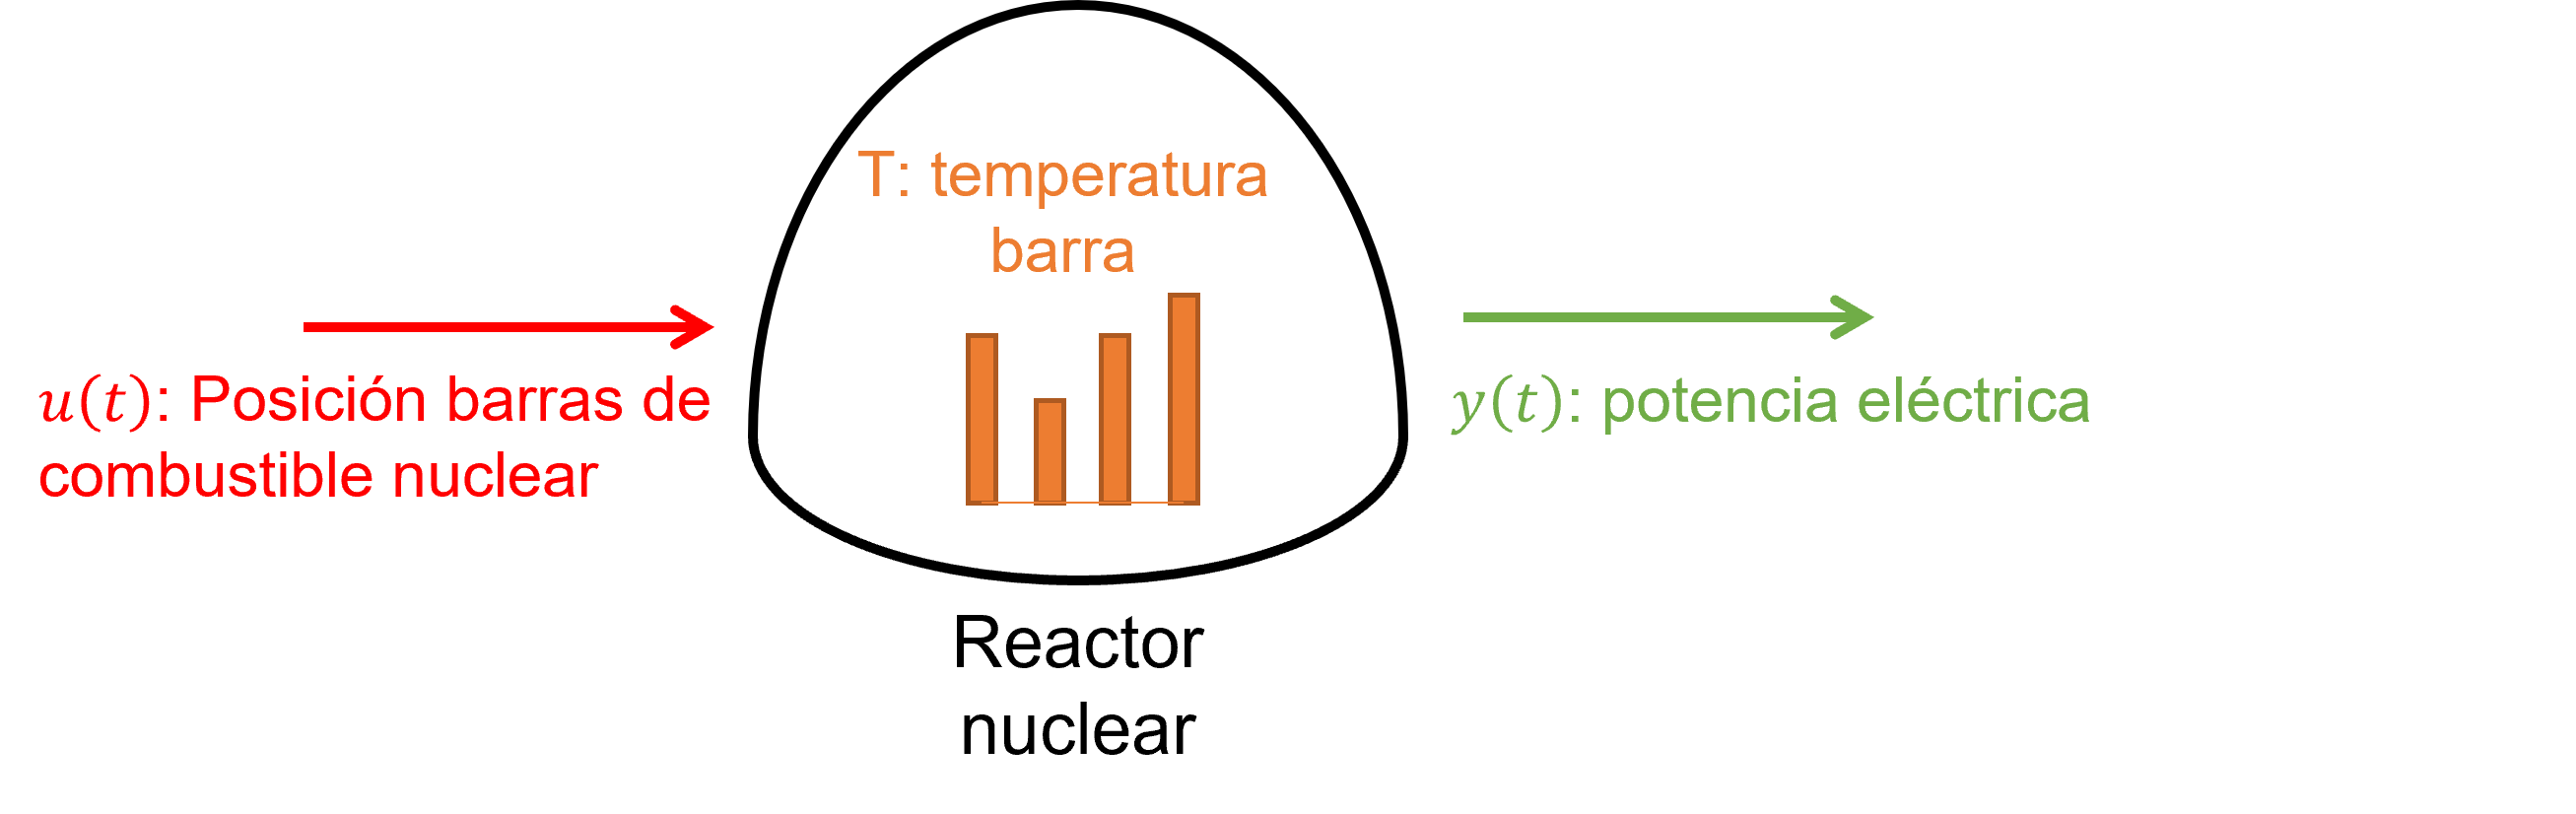
\includegraphics[scale=0.7]{Figuras/nuclear.png}
\end{figure}

¿Es posible determinar los estados internos del sistema, utilizando solo las señales de entrada y salida $\{u(t), y(t)\}$?\\
\par \underline{Respuesta}: Sí, pero con la condición que el sistema sea \textcolor{red}{observable}.\\
\par \underline{Notación}: 
\begin{itemize}
    \item $x(t)$: estados del sistema
    \item $\hat{x}(t)$: estados estimados
    \item $\tilde{x}(t)=x(t)-\hat{x}(t)$: error de estimación
\end{itemize}

\underline{Objetivo}: Diseñar un estimador/observador para $x(t)$.\\
\par Sea un sistema LTI:
\begin{align*}
    \dot{x} &= Ax+Bu\\
    y &= Cx
\end{align*}
con condición inicial $x(0)=x_0$. \\
\par Estimador: $\dot{\hat{x}}=A\hat{x}+Bu$, $\hat{x}(0)=?$ (cualquier número).\\
\par Revisemos la dinámica del error del estimador:

\begin{align*}
    \dot{\tilde{x}} &= \frac{d}{dt}(x-\hat{x})=\dot{x}-\dot{\hat{x}}\\
    &= (Ax+Bu)-(A\hat{x}+Bu)=A(x-\hat{x})
\end{align*}
Por lo tanto, $\dot{\hat{x}}=A\tilde{x}$: error del estimador posee la misma dinámica del sistema LTI.\\
\par \underline{Estrategia}: Si mis estados decaen a cero, entonces voy a diseñar un estimador tal que el error de la estimación decae con la misma tasa que el sistema.
\begin{figure}[H]
\centering
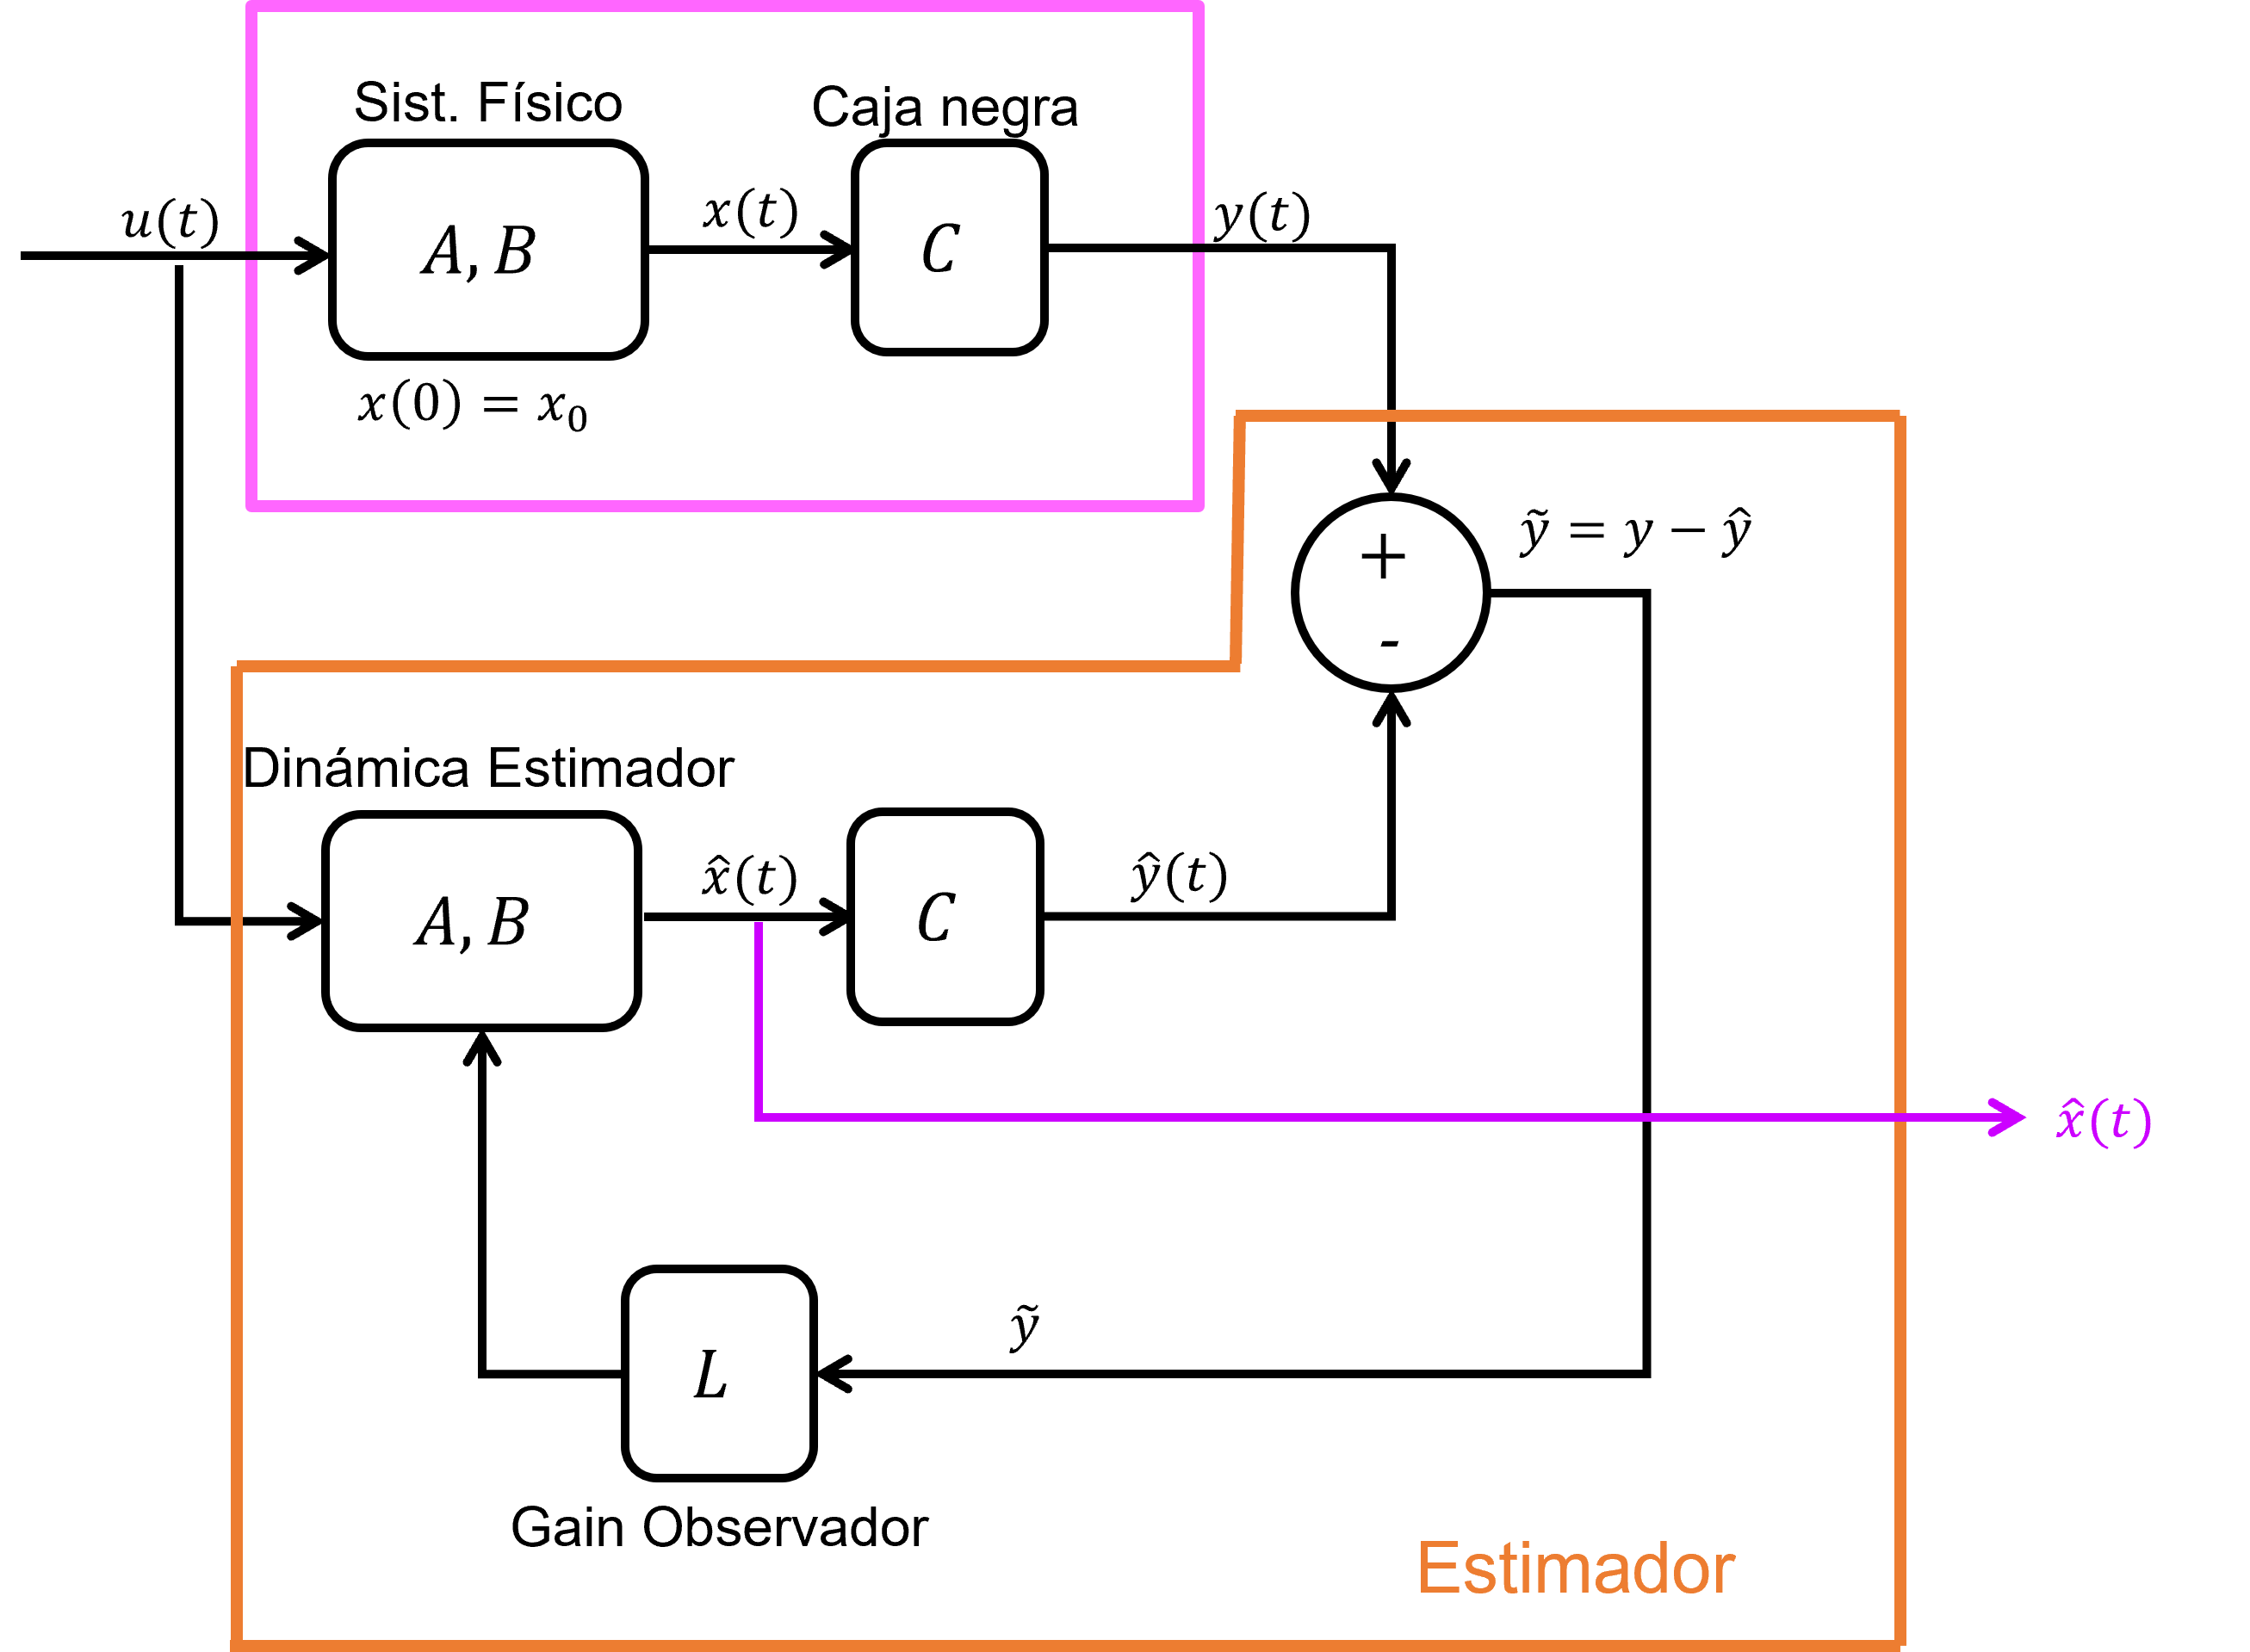
\includegraphics[scale=0.7]{Figuras/observador.png}
\end{figure}
\begin{figure}[H]
\centering
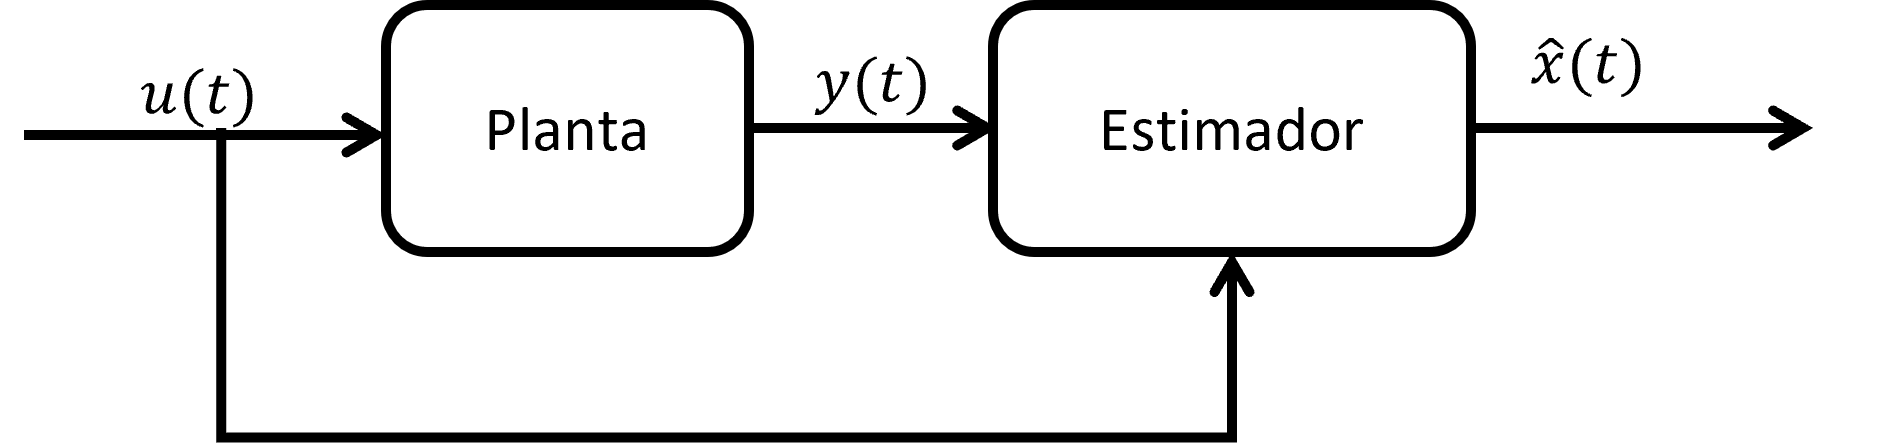
\includegraphics[scale=0.7]{Figuras/observador2.png}
\end{figure}

\section{Diseño de Observador de Estados}
\begin{align*}
    \dot{\hat{x}}=A\hat{x}+Bu+L\tilde{y}
\end{align*}
Sea 
\begin{align*}
    L=\left[
    \begin{array}{c}
     l_1 \\ l_2\\ \vdots\\ l_n 
    \end{array}\right], \quad L \in \mathbb{R}^{n\times r}, \quad x,y \in \mathbb{R}^n 
\end{align*}

Ecuación de error de estado:
\begin{align*}
    \dot{\tilde{x}}=\dot{x}-\dot{\hat{x}} &= (Ax+Bu)-(A\hat{x}+Bu+L\tilde{y})\\
    &= A\tilde{x}-L(y-\hat{y})\\
    &= A\tilde{x}-L(Cx-C\hat{x})\\
    &= A\tilde{x}-LC\tilde{x}\\
    \dot{\tilde{x}} &= (A-LC)\tilde{x}
\end{align*}
Notar que para que $(A-LC)$ cumpla estabilidad, los polos deben estar al lado izquierdo del plano complejo.\\
\par $\Longrightarrow$ Vamos a diseñar $L$, ubicando apropiadamente los polos del sistema cerrado $(A-LC)$ $\Longrightarrow$ \textcolor{red}{POLE PLACEMENT}.\\
\par \underline{Caso particular}: $x\in\mathbb{R}^n$, $u\in\mathbb{R}$, $y\in\mathbb{R}$.\\
\par Forma Canónica Observable. 
\par Recordar: 
\begin{align*}
    G(s) = \frac{b_0}{s^n+a_{n-1}s^{n-1}+...+a_1s+a_0}
\end{align*}

\begin{align*}
\tenq{A_o}=\left[
    \begin{array}{c|cccc}
     -a_{n-1} & 1 & & & 0 \\ 
     -a_{n-2} & & 1 & & \\
     \vdots   & & & \ddots & \\
     -a_1     & 0 & & & 1 \\ \hline
     -a_0     & 0 & 0 & \dots & 0   
    \end{array}\right], \quad \tenq{A_o}\in \mathbb{R}^{n\times n}
\end{align*}
\begin{align*}
\tenq{B_o}=\left[
    \begin{array}{c}
     b_{n-1} \\
     b_{n-2}\\
    \vdots\\
     b_1 \\ \hline
     b_0
    \end{array}\right], \quad \tenq{B_o}\in \mathbb{R}^{n\times 1}
\end{align*}
\begin{align*}
\tenq{C_o}=\left[
    \begin{array}{c|ccc}
     1 & 0 & \dots & 0
    \end{array}\right], \quad \tenq{C}_o\in \mathbb{R}^{1\times n}
\end{align*}
Si $y\in\mathbb{R}$, entonces:
\begin{align*}
    L=\left[
    \begin{array}{c}
     l_{n-1} \\ l_{n-2}\\ \vdots\\ l_0 
    \end{array}\right] 
\end{align*}
\underline{Objetivo}: Determinar los $l_i$, $i\in[0,n-1]$
\begin{align*}
    LC_o&=\left[
    \begin{array}{c}
     l_{n-1} \\ l_{n-2}\\ \vdots\\ l_0 
    \end{array}\right] \left[
    \begin{array}{c c c c}
     1 & 0 & ... & 0
    \end{array}\right] =\left[
    \begin{array}{c|c}
     l_{n-1} & \\ \vdots & \tenq{0} \\ l_0 & 
    \end{array}\right] \\
    A_o-LC_o &= \left[ \begin{array}{c|c c c}
     -a_{n-1}-l_{n-1} & & & \\  -a_{n-2}-l_{n-2} & & & \\ \vdots & & \tenq{I} & \\-a_1-l_1 & & & \\ \hline \\ -a_0-l_0 & 0 & ... & 0
    \end{array}\right] 
\end{align*}
Ecuación característica: 
\begin{align*}
    \Delta(A_o-LC_o) =s^n+(a_{n-1}+l_{n-1})s^{n-1}+...+(a_1+l_1)s+(a_0+l_0)=0    
\end{align*}
donde $\lambda_i=(a_i+l_i)$, $i\in[0,n-1]$, son los coeficientes del polinomio característico, asociado a la ubicación de polos deseada:
\begin{align*}
    \prod_{i=0}^{n-1}(s-p_i)=s^n+\lambda_{n-1}s^{n-1}+...+\lambda_1s+\lambda_0=0
\end{align*}
donde $p_i$ es la posición de los polos deseada.\\
\par Finalmente:
\begin{align*}
    l_i=a_i-\lambda_i,\quad i\in[0,n-1]
\end{align*}
\par \underline{Nota}: en Matlab, utilizar el comando \texttt{place()}. \\
\par \underline{Nota}: Si el sistema no está escrito en OCF, entonces se puede realizar una transformación de similitud con matriz T. Esta matriz T existe ssi el sistema es observable.

\section{Principio de Separación}
Estudiemos el siguiente sistema LTI cerrado:
\begin{figure}[H]
\centering
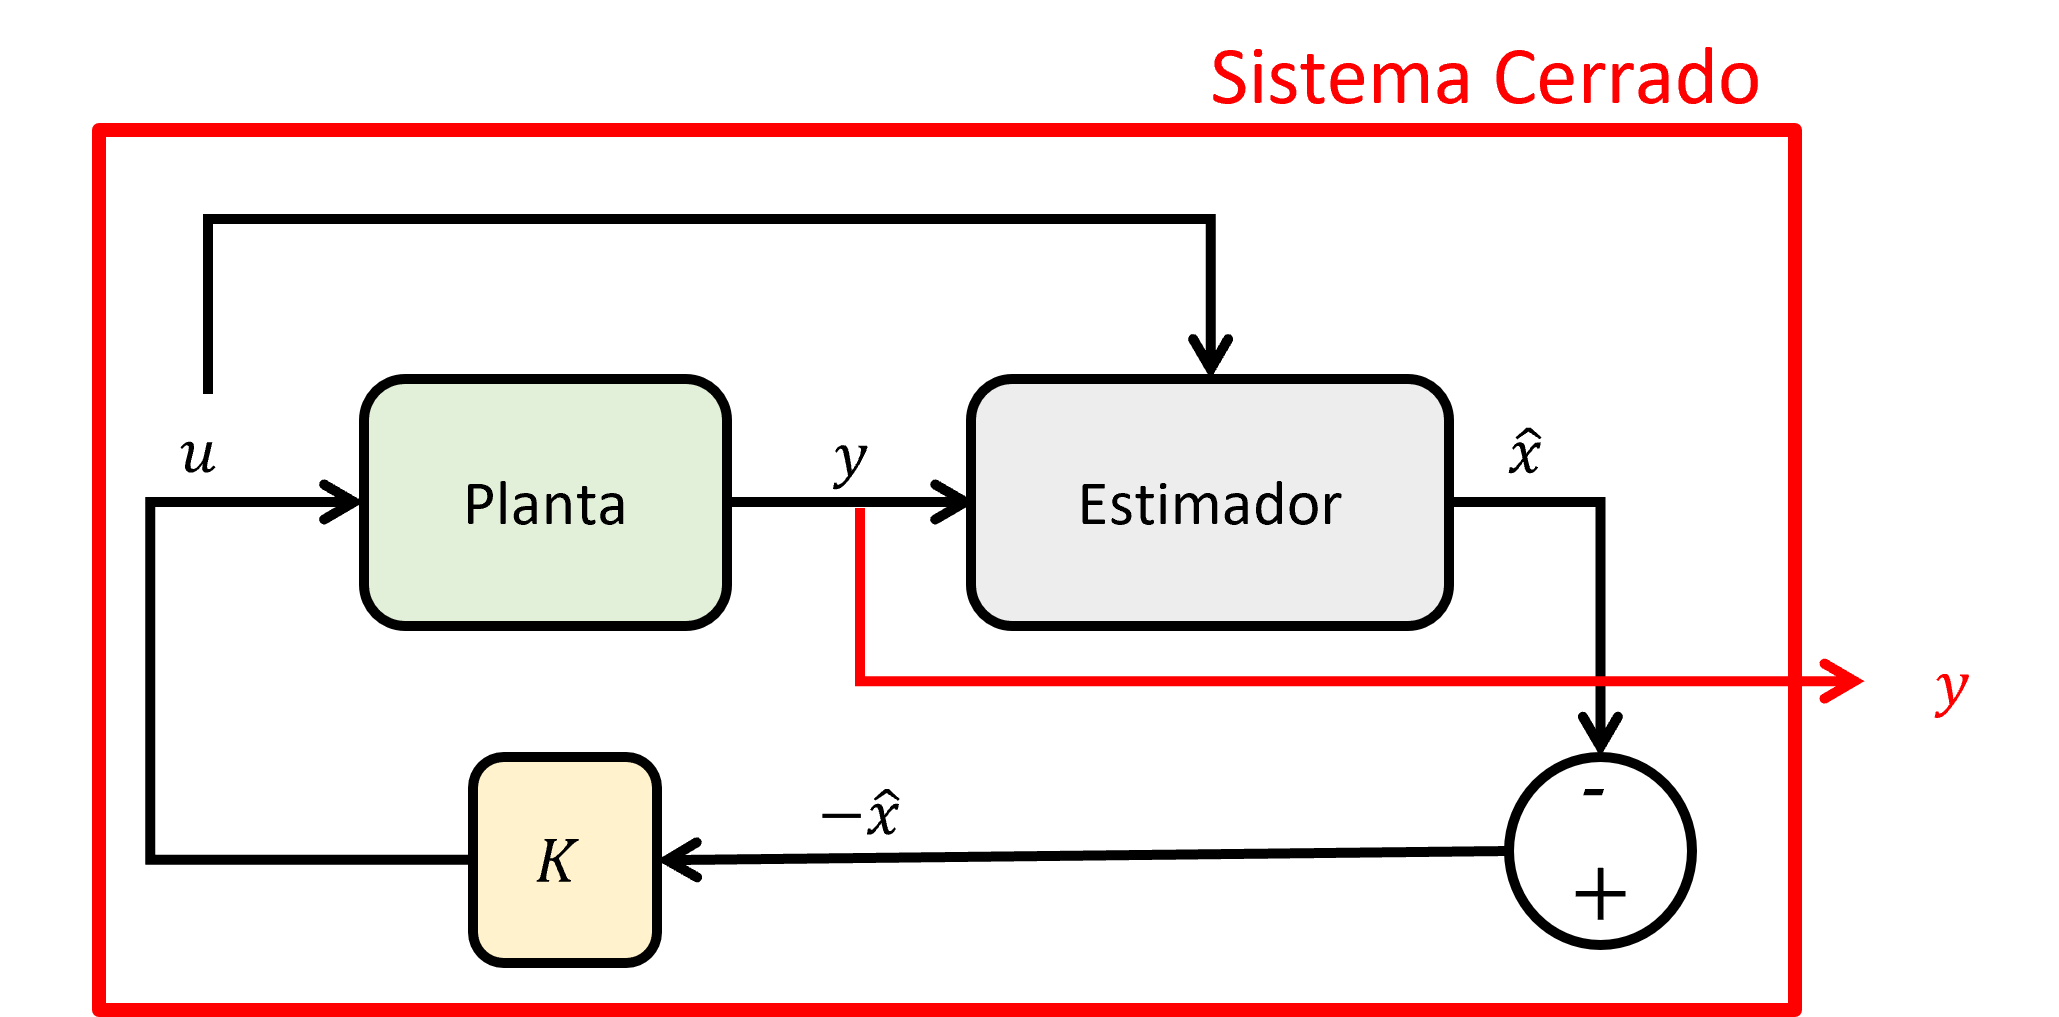
\includegraphics[scale=0.7]{Figuras/ppio_separacion.png}
\end{figure}

\setcounter{equation}{0}
\begin{subequations}
\begin{align}
    \text{Planta: }  \dot{x} &= Ax+Bu\\
    y &= Cx
    \end{align}
\end{subequations}
\begin{subequations}
    \begin{align}
    \text{Controlador: }  u &= -k\hat{x}
    \end{align}
\end{subequations} 
\begin{subequations}
    \begin{align}
    \text{Estimador: }  \dot{\hat{x}}&= A\hat{x}+Bu+L\tilde{y}\\
     \hat{y} &= C\hat{x}\\
     \tilde{x} &= x-\hat{x}\\
    \tilde{y} &= y-\hat{y}
\end{align}
\end{subequations}

Vamos a obtener una expresión para el sistema cerrado:
\begin{align}
    \text{(3.2a) y (3.3c):} \quad u&=-K(c-\tilde{x})\\
    \text{(3.4) y (3.1a):} \quad \dot{x} &= Ax-BK(x\tilde{x})\\
    \Longrightarrow \dot{x} &= (A-BK)x+BK\tilde{x}\\
    \text{(3.3c) y (3.3a):} \quad \tilde{x} &= x-\hat{x}\\
    \dot{\tilde{x}} &= \dot{x}-\dot{\hat{x}}\\
    \Longrightarrow \dot{\tilde{x}} &= (Ax+Bu)-(A\hat{x}+Bu+L\tilde{y})\\
    \Longrightarrow \dot{\tilde{x}} &= A\tilde{x}-LC \tilde{x}\\
    \Longrightarrow \dot{\tilde{x}} &= (A-LC)\tilde{x}
\end{align}
Definir $z=\left[
    \begin{array}{c}
     x \\ \tilde{x} 
    \end{array}\right]$, estados del sistema cerrado.\\
\par Ecuación de estado del sistema cerrado:
\begin{align*}
    \dot{z}=\left[
    \begin{array}{c}
     \dot{x} \\ \dot{\tilde{x}} 
    \end{array}\right] = \left[
    \begin{array}{cc}
     A-BK & BK \\ 0 & A-LC 
    \end{array}\right]\left[
    \begin{array}{c}
     x \\ \tilde{x} 
    \end{array}\right]
\end{align*}
Definimos:
\begin{align*}
    A_{CL} &= \left[
    \begin{array}{cc}
     A-BK & BK \\ 0 & A-LC 
    \end{array}\right]\\
    \Longrightarrow \dot{z}&=A_{CL}z
\end{align*}

Los polos de $A_{CL}$ se obtienen al resolver la ecuación característica:
\begin{align*}
    \text{det}(sI-A_{CL})&=0\\
    \Longrightarrow \text{det}(sI-(A-BK))\cdot\text{det}(sI-(A-LC)) &=0
\end{align*}
\begin{itemize}
    \item $\text{det}(sI-(A-BK))$: polos del subsistema planta + controlador
    \item $\text{det}(sI-(A-LC))$: polos del subsistema planta + observador 
\end{itemize}

Este resultado se conoce como el \textcolor{red}{principio de separación}.\\
\par Diseñar $K$ y $L$ por separado, luego agrupar y construir el sistema de control cerrado.




%----------- Cap4 -----------%
\input{Capitulos/Control_optimo}

%----------- Cap5 -----------%
\chapter{Vibraciones Estocásticas}


\section{Proceso Estocástico}
Primera, una \textcolor{red}{variable aleatoria} $X$ toma un valor de ``realización'', no hay un efecto del tiempo.

\par Ejemplos:
\begin{itemize}
    \item Período de retorno (``ocurrencia'') de un terremoto
    \item Módulo de Young (concreto)
    \item Resistencia característica (acero, $F_y$)
    \item Geometría
\end{itemize}

Un \textcolor{red}{proceso estocástico} es una familia de variables aleatorias cuya realización depende del tiempo.\\
$X(t)$, $t\in T$ es un proceso estocástico (p.e.) 
$$\Longrightarrow \{X(t_1),X(t_2),X(t_3),...\}$$

Realización 1: 
\begin{figure}[H]
\centering
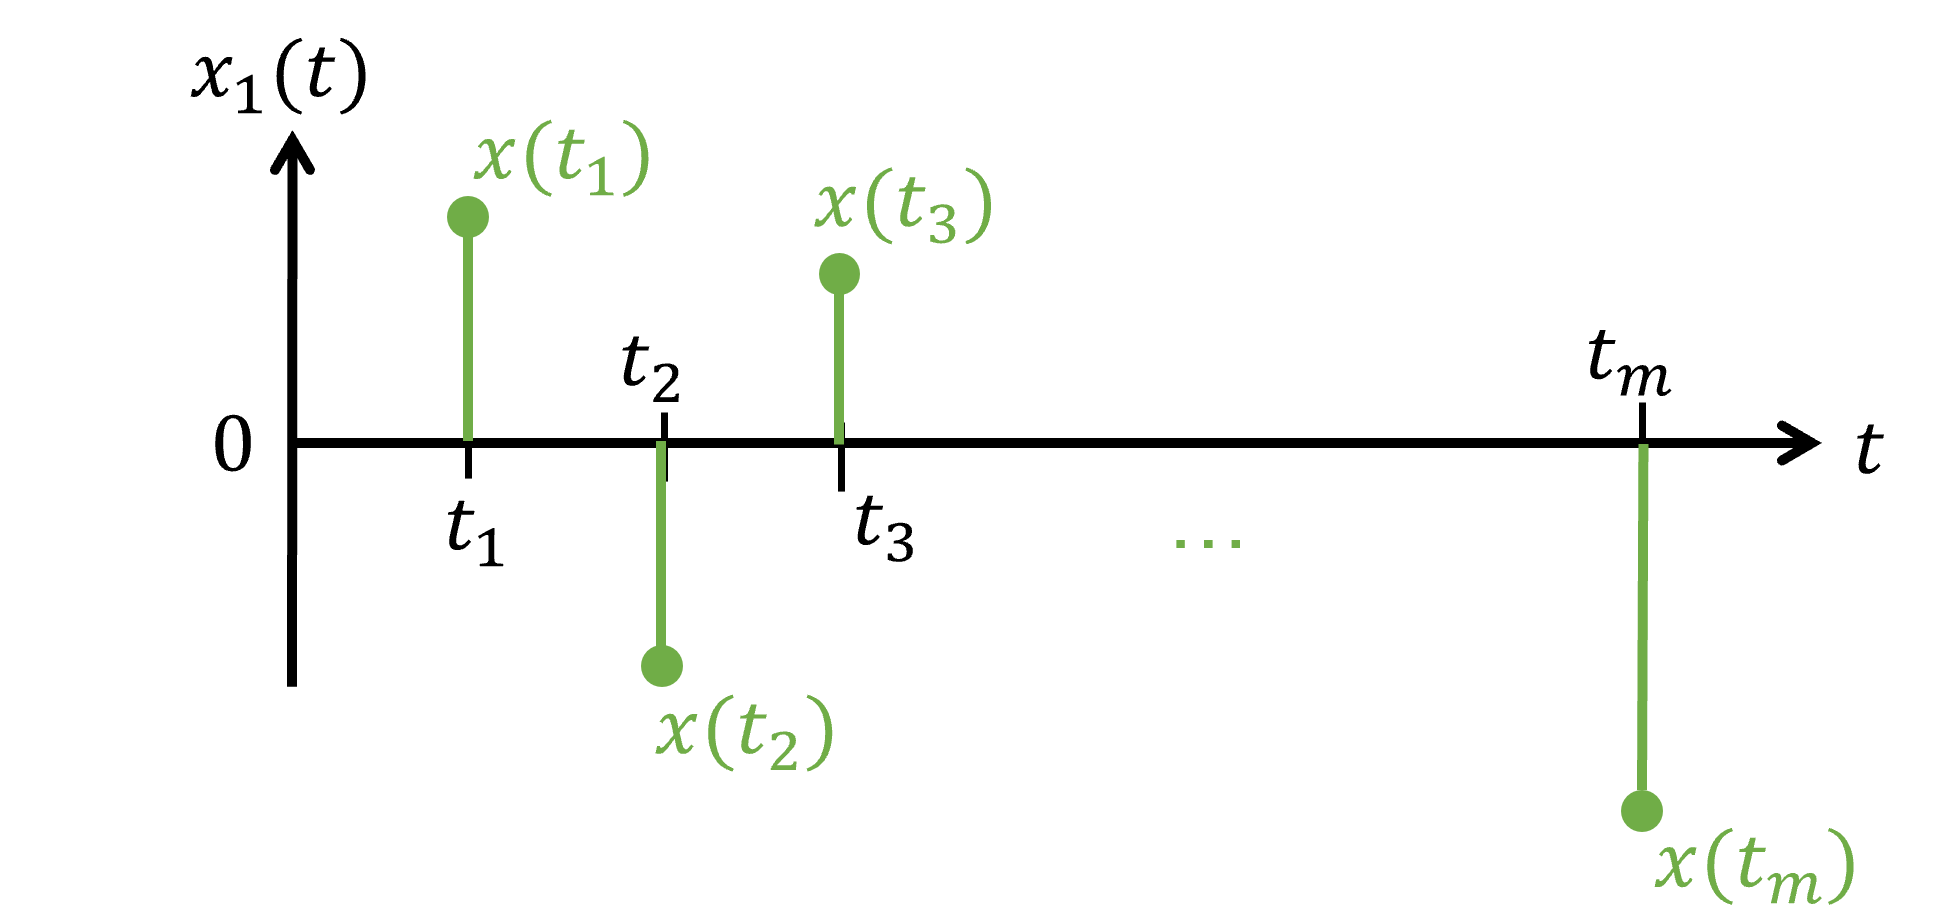
\includegraphics[scale=0.7]{Figuras/pe.png}
\end{figure}

Realización 2: 
\begin{figure}[H]
\centering
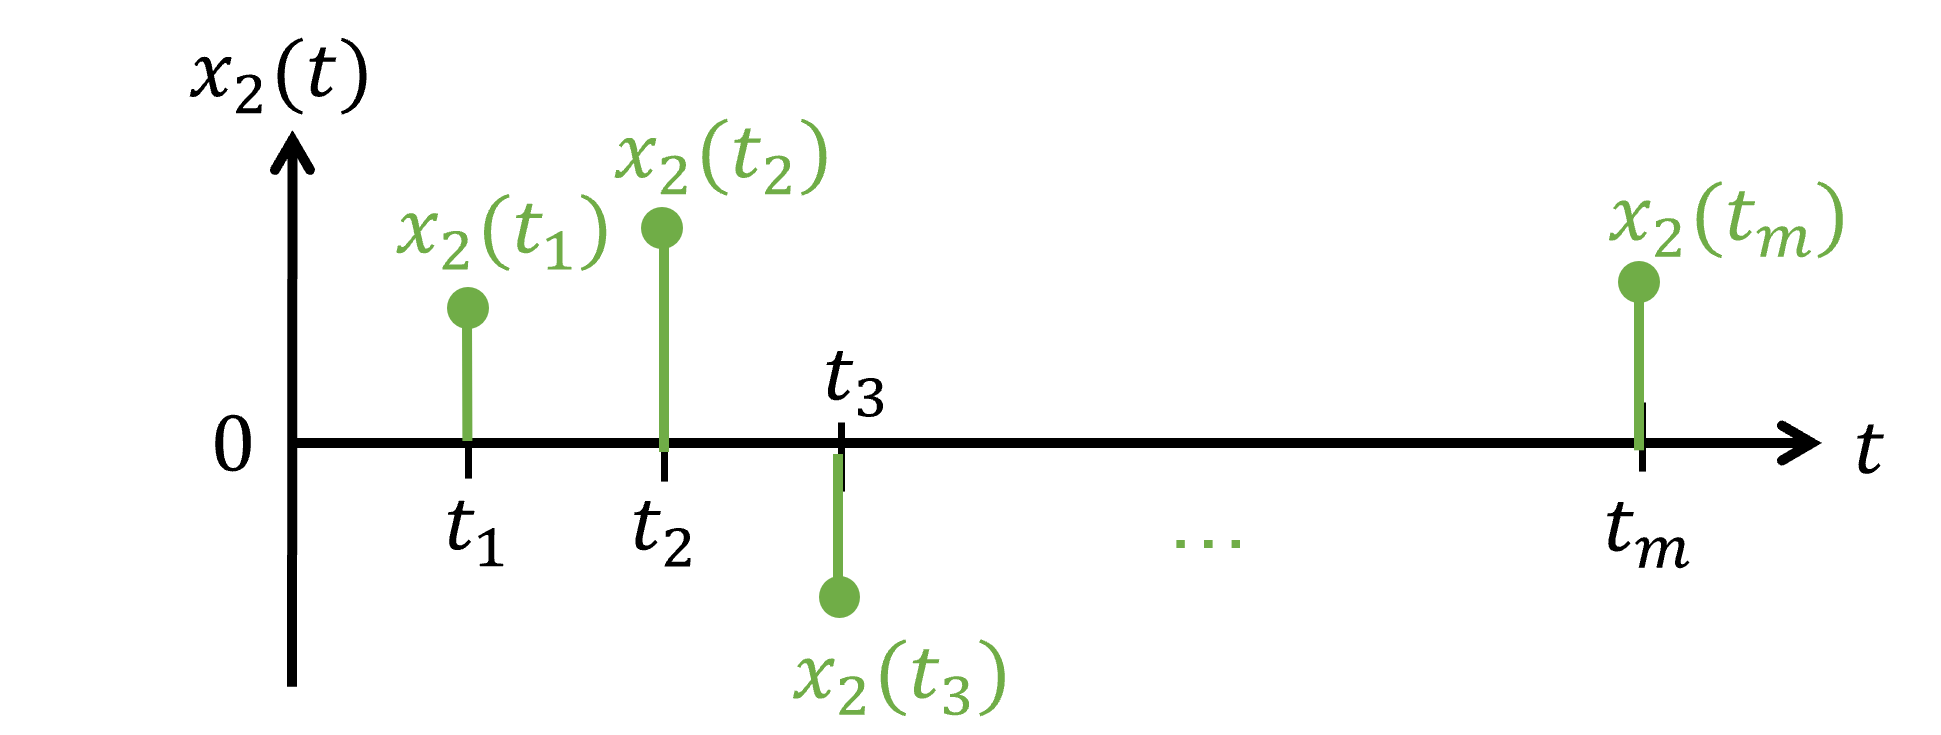
\includegraphics[scale=0.7]{Figuras/pe2.png}
\end{figure}


\par Ejemplos:
\begin{itemize}
    \item Registro de aceleración de un terremoto
    \item Presión del viento
    \item Aceleración de piso de un edificio
\end{itemize}

\par Considere un p.e. escalar $X(t)$, $t\in T$.\\
\par Existen 2 formas de describir un p.e.:
\begin{enumerate}
    \item Función de densidad de probabilidad
    \begin{align*}
        \mathbb{P}[X(t_1)\leq x_1 \cap X(t_2)\leq x_2 \cap ... \cap X(t_m) \leq x_m ] = F_m(x_1,x_2,...,x_m;t_1,t_2,...,t_m)
    \end{align*}
    \item Momentos estocásticos $\Longrightarrow$ momentos de 1er y 2do orden
    \begin{itemize}
        \item Media: $$\mu _X(t)=\mathbb{E}\{X(t)\}$$
        \item Varianza: $$\rho _X^2(t)=\mathbb{E}\{[X(t)-\mu_X(t)]^2\}$$
        \item Función de auto-correlación: $$R_{XX}(t_1,t_2)=\mathbb{E}\{X(t_1)X(t_2)\}$$
        \item Función de auto-covarianza: $$\Gamma_{XX}=\mathbb{E}\{[X(t_1)-\mu_X(t_1)][X(t_2)-\mu_X(t_2)]\}$$ $$\Gamma_{XX}=R_{XX}(t_1,t_2)-\mu_X(t_1)\mu_X(t_2)$$
        \item Coeficiente de correlación: $$\rho_{XX}(t_1,t_2) = \frac{\Gamma_{XX}(t_1,t_2)}{\sigma_X(t_1)\sigma_X(t_2)}$$
        Interpretación: ``medida de independencia lineal entre variables aleatorias''. \\
        \begin{figure}[H]
        \centering
        \subfigure[]{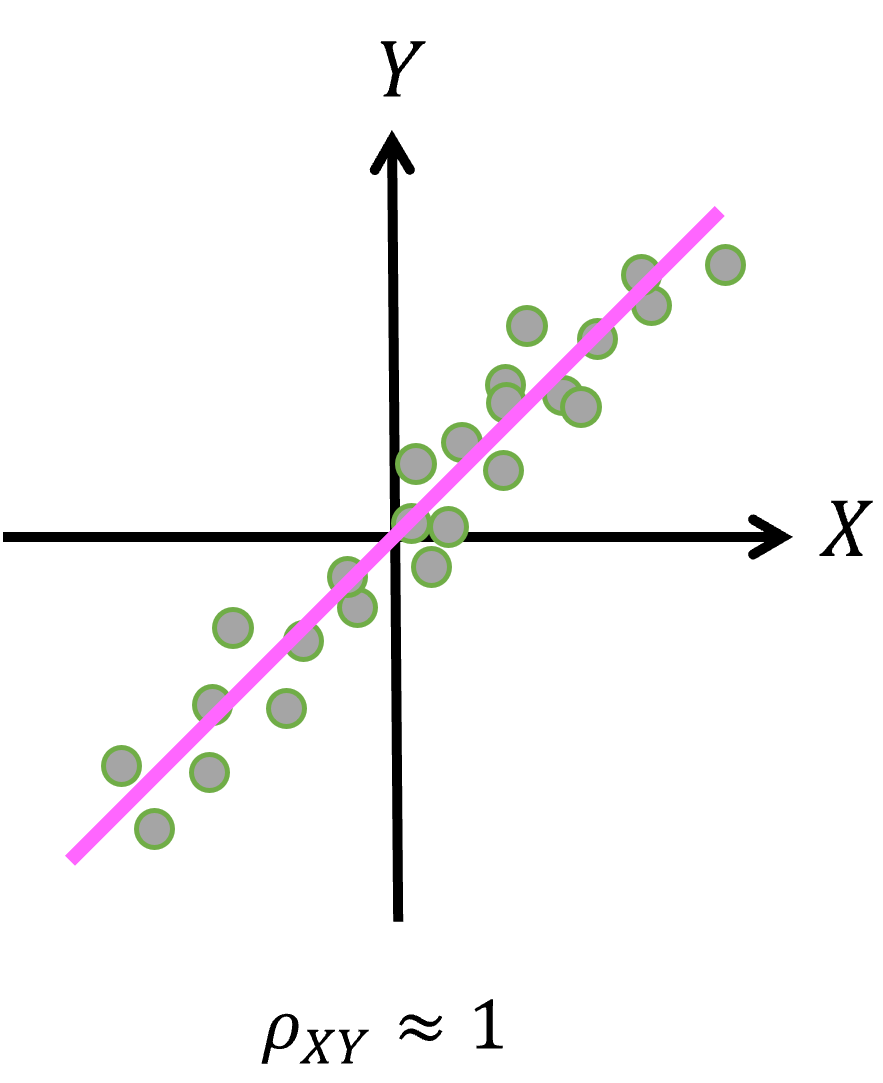
\includegraphics[scale=0.7]{Figuras/rho1.png}}
        \subfigure[]{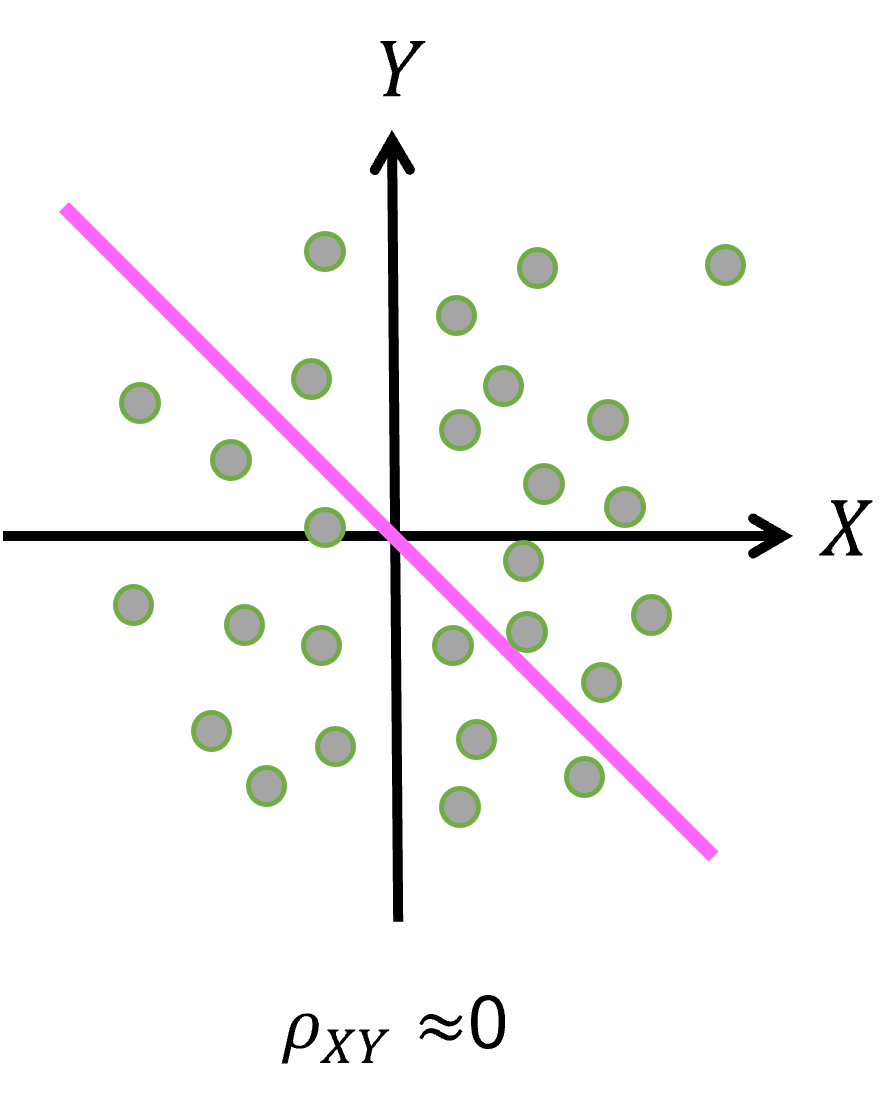
\includegraphics[scale=0.7]{Figuras/rho0.png}}
        \end{figure}
        Notas: \begin{itemize}
            \item $|\rho_{XX}(t_1,t_2)| \leq 1$
            \item Si $\rho_{XX}(t_1,t_2)=0$, $\forall t_1 \neq t_2$, entonces el p.e. es un proceso descorrelacionado (ruido blanco, por ejemplo).
        \end{itemize} 
    \end{itemize}
\end{enumerate}

Otras definiciones importantes:\\
\par Sean $X(t)$ y $Y(t)$ dos procesos estocásticos, $t\in T$:
\begin{itemize}
    \item Función de correlación cruzada: $$R_{XY}(t_1,t_2)=\mathbb{E}\{X(t_1)Y(t_2)\} $$
    \item Función de covarianza cruzada:
    $$\Gamma_{XY}(t_1,t_2) =\mathbb{E}\{ [X(t_1)-\mu_x(t_1)][Y(t_2)-\mu_y(t_2)]\} $$
    $$\Gamma_{XY}(t_1,t_2) = R_{XY}-\mu_X(t_1)\mu_Y(t_2) $$ 
    \item Coeficiente de correlación cruzado: $$\rho_{XY}(t_1,t_2)=\frac{\Gamma_{XY}(t_1,t_2)}{\sigma_x(t_1)\sigma_y(t_2)} $$
\end{itemize}

\section{Clasificación de P.E.}
\begin{enumerate}
    \item P.E. no estacionario:
    \begin{itemize}
        \item La distribución de probabilidad del p.e. depende del tiempo.
    \end{itemize}
    \begin{figure}[H]
    \centering
    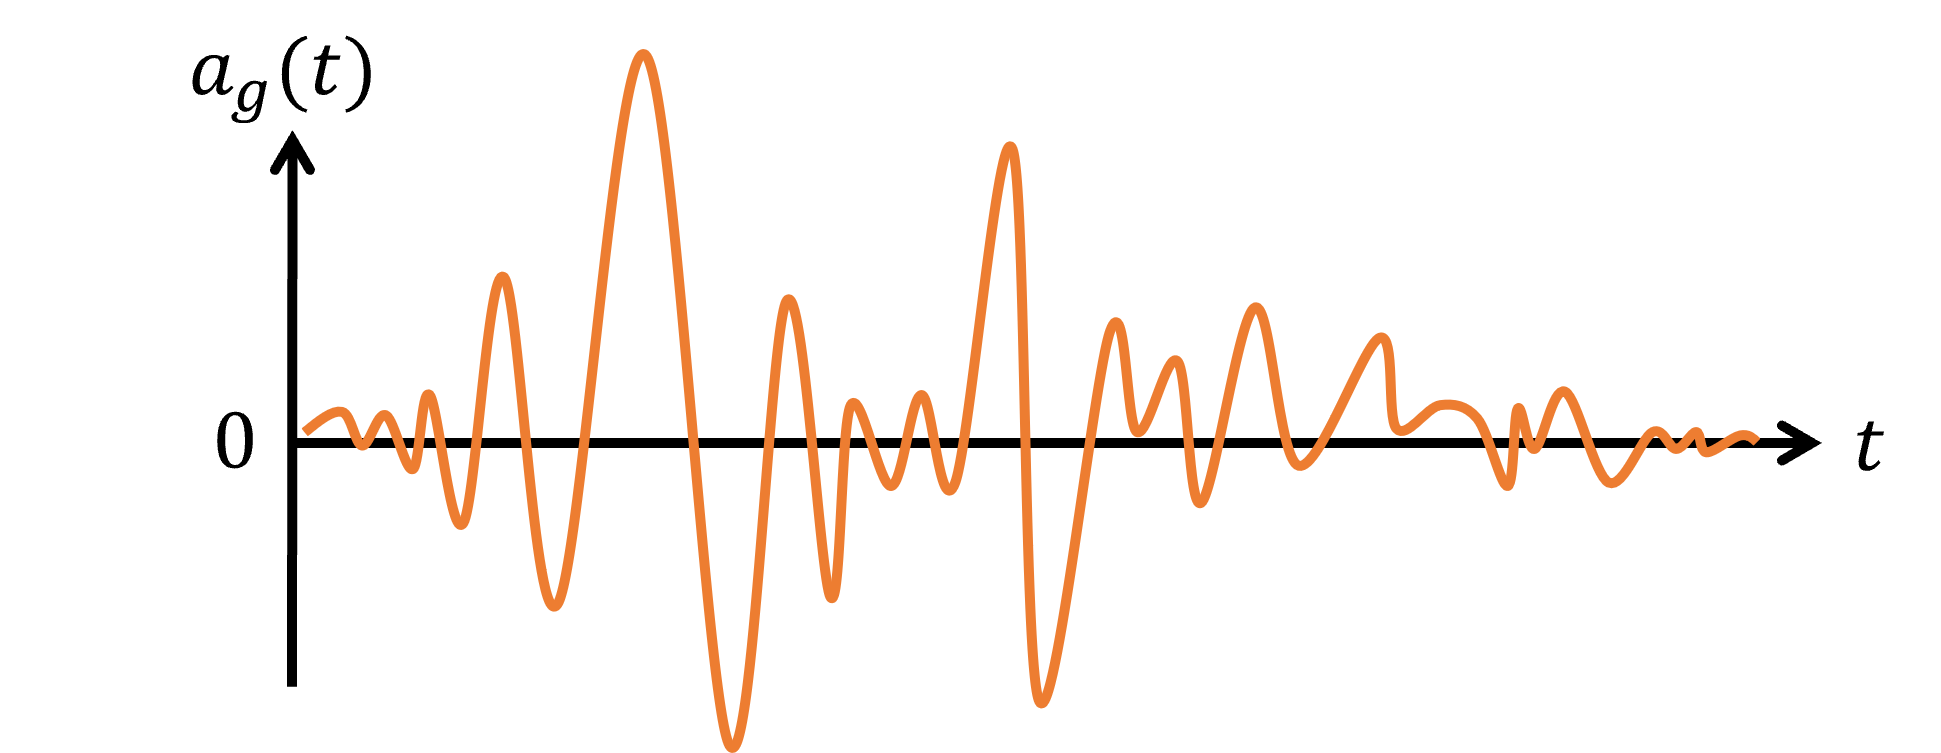
\includegraphics[scale=0.7]{Figuras/penoesatacionario.png}
    \end{figure}
    \item P.E. Estrictamente estacionario:
    \begin{itemize}
        \item La distribución de probabilidad del p.e. no cambia con un retraso en el tiempo:
        \begin{equation*}
            F_X(x_1,...,x_m;t_1,...,t_m)=F_x(x_1,...,x_m;\textcolor{brown}{t_1+\tau,...,t_m+\tau})
        \end{equation*}
    \end{itemize}
    \begin{figure}[H]
    \centering
    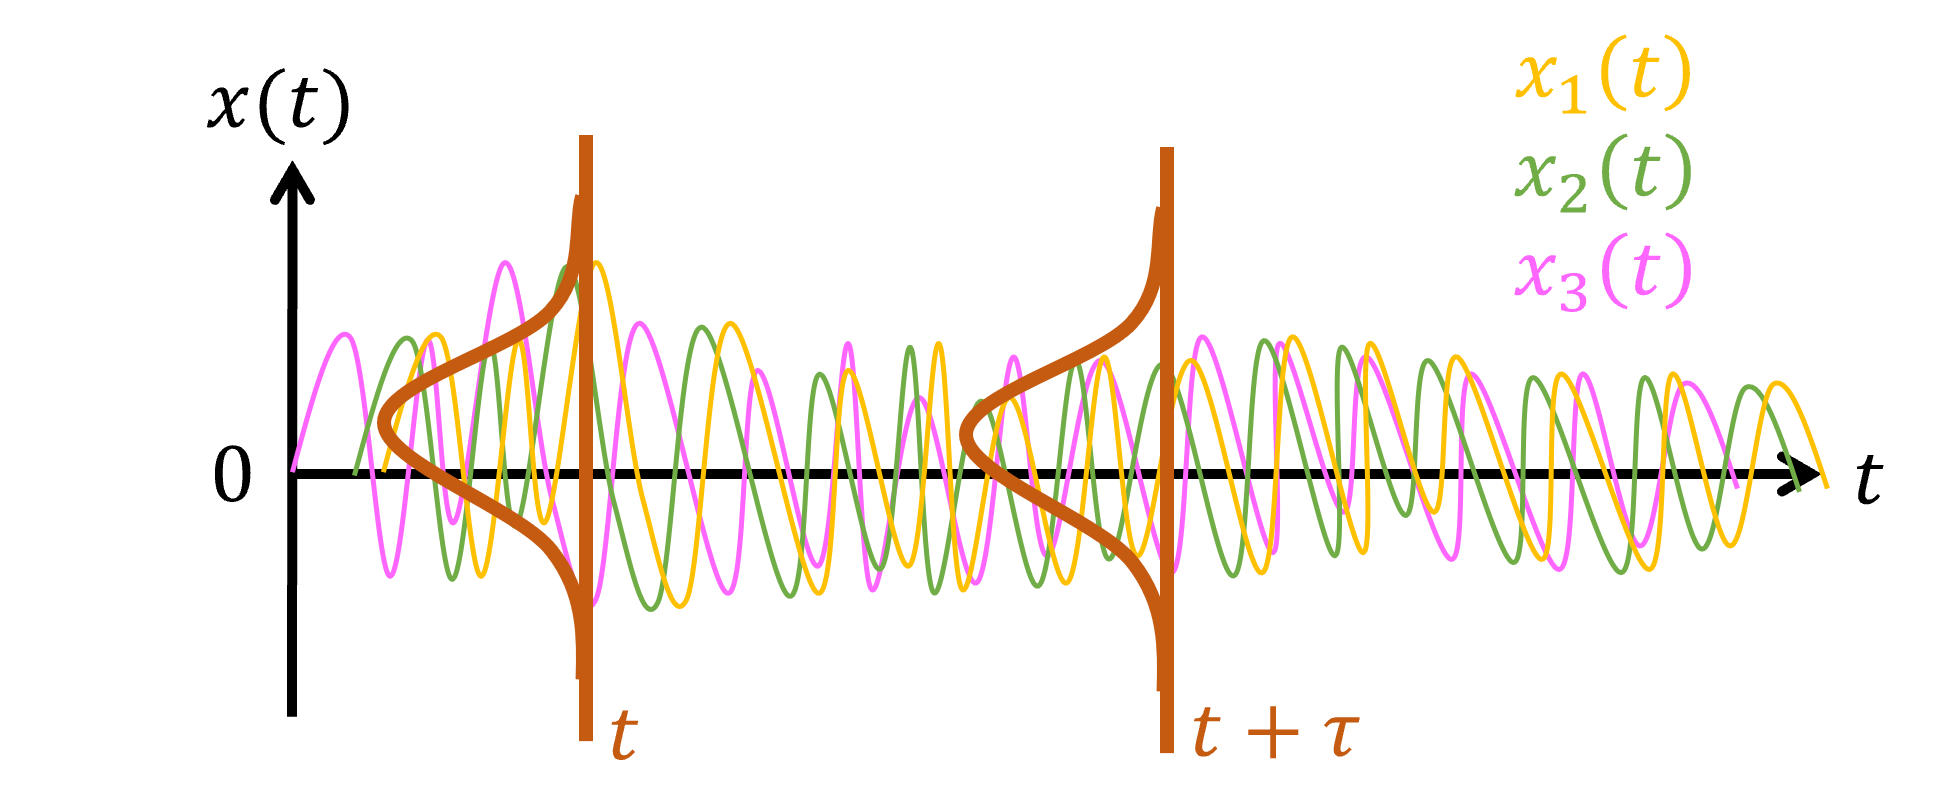
\includegraphics[scale=0.7]{Figuras/peestricto.png}
    \end{figure}
    \item P.E. Débilmente estacionario:
    \begin{itemize}
        \item Estadísticos de 2do orden son finitos y no varían en el tiempo
        \begin{align*}
            \mu_x(t)&=\mu_x<\infty, \quad \sigma_x^2(t)=\sigma_x^2<\infty\\
            \Longrightarrow R_{XX}(t_1,t_2)=R_{XX}(t_2-t_1)
        \end{align*}
    \end{itemize}
\end{enumerate}

\section{P.E. Gaussiano}
Un p.e. $X(t)$, $t \in T$, se llama un p.e. Gaussiano si, para cada conjunto $\{t_1,t_2,...,t_m\}\in T$, las ``m'' variables aleatorias $X(t_1)$, $X(t_2)$, $...,$ $X(t_m)$ son distribuidas normales multivariadas.
\begin{align*}
    X(t)\sim~ N\big(\mu_X(t),\Gamma_{XX}(t_i,t_j)\big)
\end{align*}

\underline{Notas}:
\begin{itemize}
    \item Un p.e. Gaussiano y débilmente estacionario es estrictamente estacionario.
    \item Un p.e. Gaussiano preserva las transformaciones lineales, y esto es extremadamente útil en los problemas de sistemas lineales que se verán más adelante.
\end{itemize}





\section{Densidad de Poder Espectral (power spectral density, PSD)}
Dado X un w.s.s., la función de autocorrelación se define como:
\begin{align*}
    R_X(\tau)=\mathbb{E}\{X(t)X(t+\tau)\}
\end{align*}

Características de $R_X$:
\begin{enumerate}
    \item $R_X(\tau)$ es una función par $\longrightarrow$ simetría
    \begin{align*}
        R_X(\tau)=R_X(-\tau)
    \end{align*}
    \item $R_X(\tau)$ debe ser finita. Adicionalmente.:
    \begin{align*}
        |R_X(\tau)|&\leq R_X(0)\\
        \Longrightarrow R_X(0)&=\mathbb{E}\{X^2(t)\}=\sigma^2_X(t)+\mu_X^2(t)
    \end{align*}
    En $\tau=0$, $R_X(0)$ nos entrega el máximo valor de la media cuadrada del p.e. X.
    \item $R_X(\tau)$ es una función definida positiva.\\
    $\Longrightarrow$ Para cualquier función $g(t)$, si:
    \begin{align*}
        g(t_1)R_X(t_1-t_2)g(t_2)\geq 0
    \end{align*}
    Por lo tanto, $R_X(\tau)$ es definida positiva siempre.
    \item $R_X(\tau)$ es continua en $\tau$.
\end{enumerate}

\underline{Definición}: Densidad de poder espectral.\\
\par Sea $X=(X(t):t\in T)$ un p.e. w.s.s., con función de autocorrelación $R_x(\tau)$. La función de densidad de poder espectral se define como (Teorema de Wiener-Khintchine):
\begin{align*}
    S_X(\omega) &=\mathcal{F}\{R_X(\tau)\}\\
    R_X(\tau) &=\mathcal{F}^{-1}\{S_X(\omega)\}
\end{align*}
Nota: En inglés, Power Spectral Density (PSD).\\
\par \underline{Propiedades PSD}:
\begin{enumerate}
    \item Función real
    \item Función simétrica
    \item Definida positiva
    \item Área bajo la curva de $S_X(\omega)$ es igual a l valor medio cuadrado
\end{enumerate}
\begin{figure}[H]
\centering
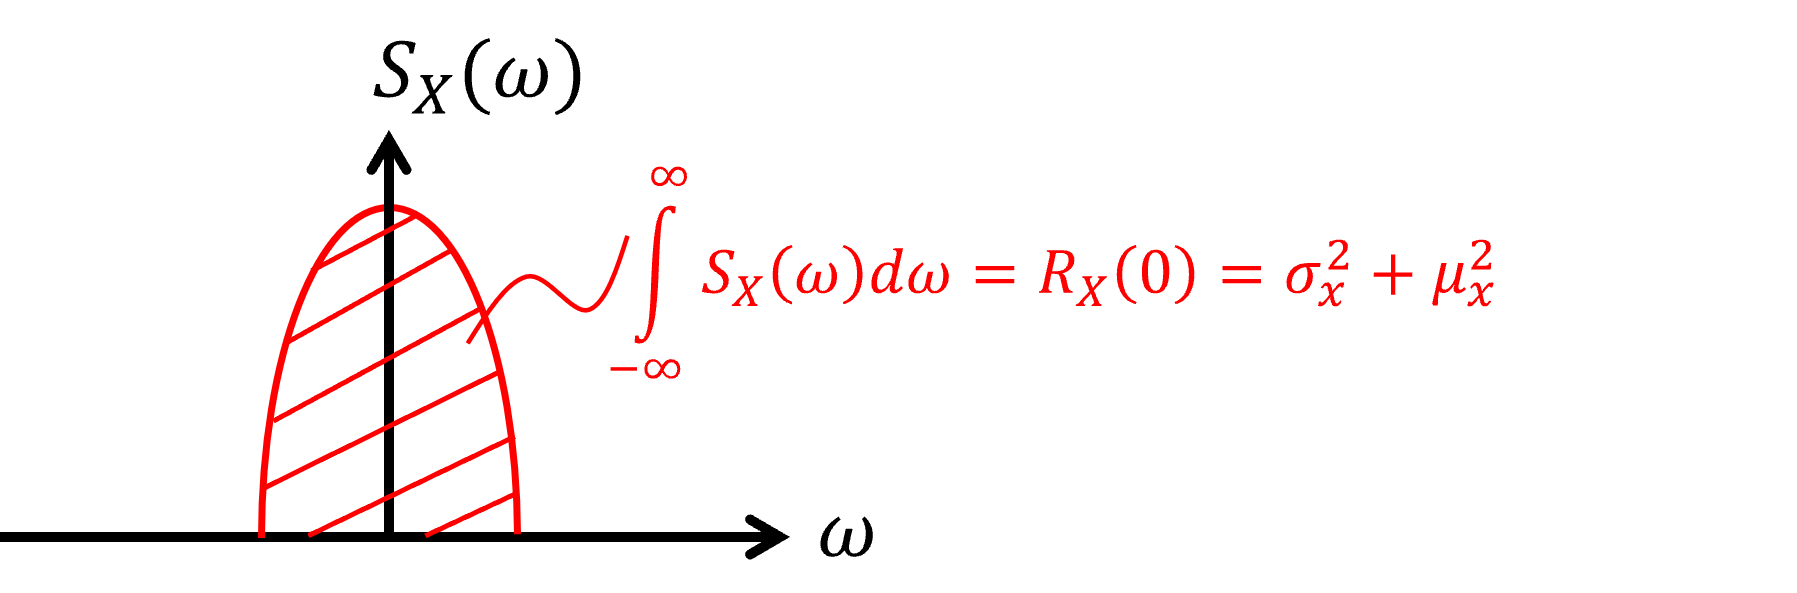
\includegraphics[scale=0.7]{Figuras/PSD.png}
\end{figure}

\section{Ruido blanco}
Sea $X=(X(t), t\in T)$ un p.e. w.s.s., con media 0, $\mu_x=0$, X es un ruido blanco si su PSD es constante:
\begin{align*}
    S_X(\omega) &= S_0, \quad \forall \omega \in (-\infty,+\infty)\\
    R_X(\tau) &= 2\pi S_0\delta (\tau)
\end{align*}

\underline{Nota}: Un ruido blanco es un p.e. Gaussiano.
\begin{figure}[H]
\centering
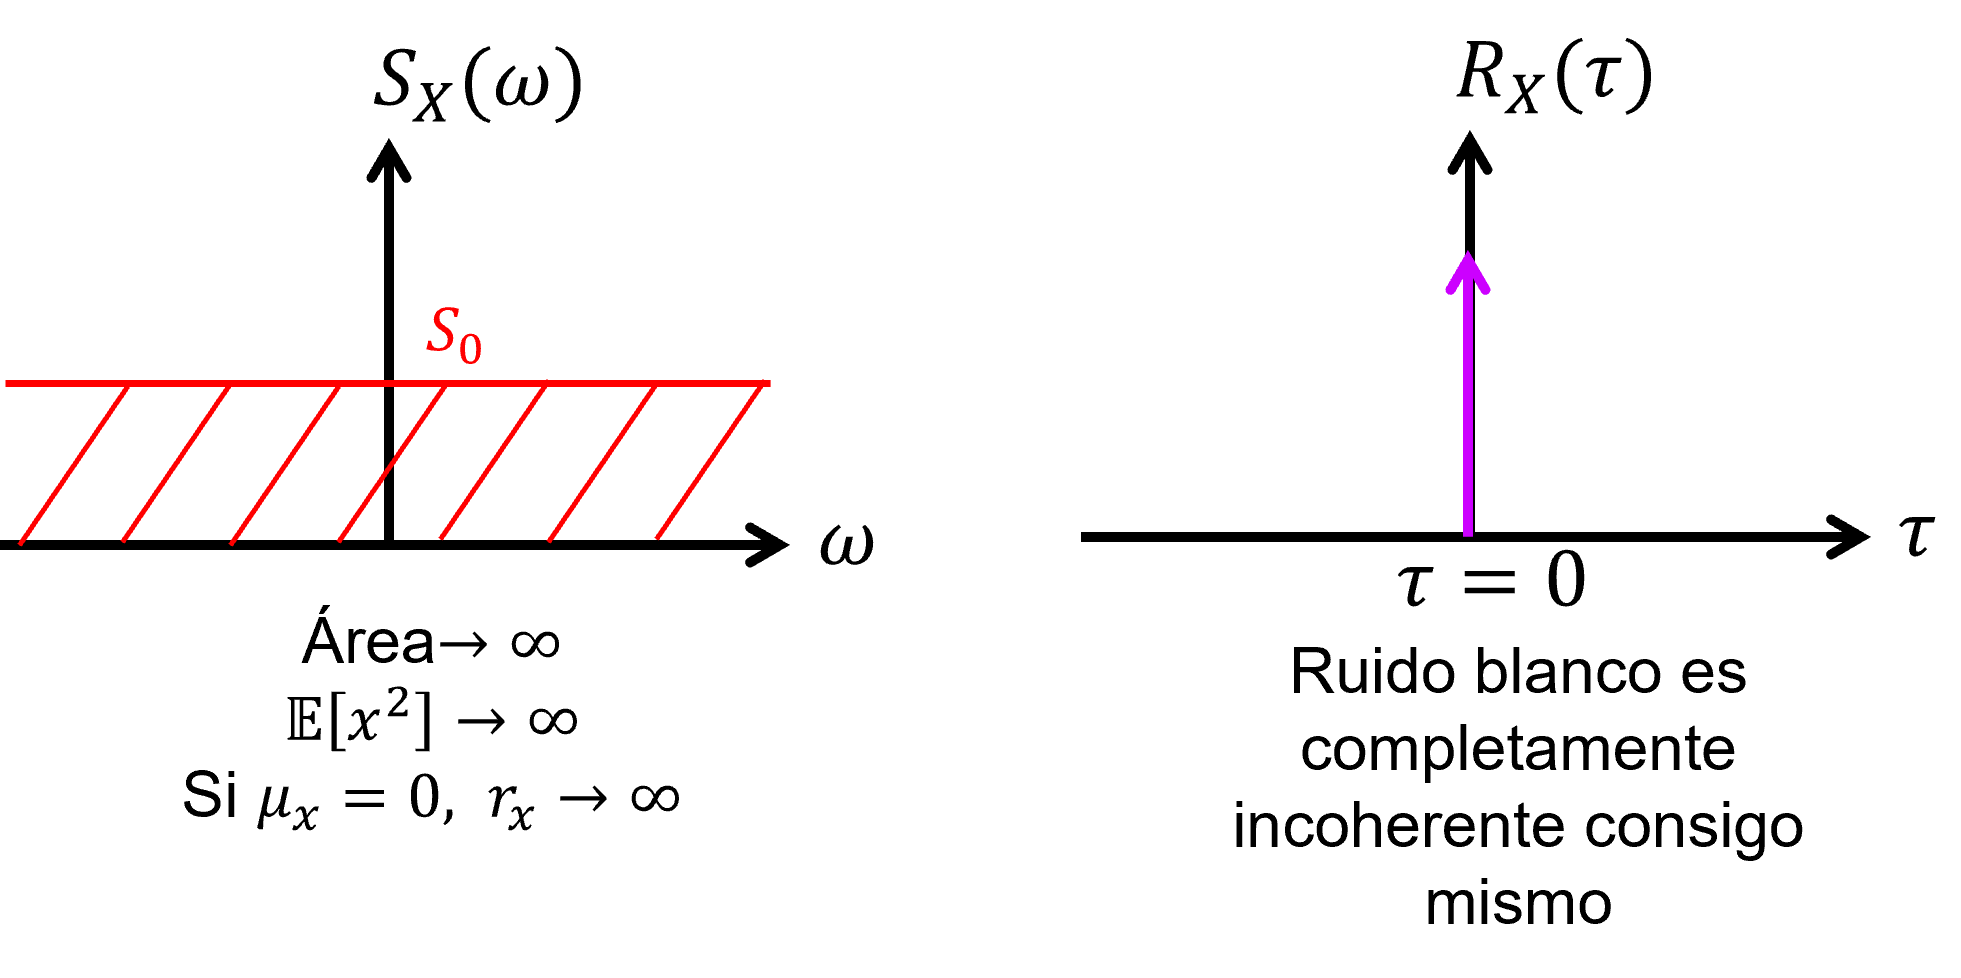
\includegraphics[scale=0.7]{Figuras/ruidoblanco.png}
\end{figure}


\section{Ruido blanco de banda limitada (band-limited white noise, BLWN)}
Sea X un p.e., w.s.s., es un BLWN si:
\begin{align*}
    S_X(\omega) & = \left\{
\begin{array}{ll}
      S_0 & |\omega|\leq \omega_c \\
      0 & |\omega|> \omega_c \\
\end{array} 
\right. \\
    R_X(\tau) & = R(0)\frac{\sin(\omega_c \tau)}{\omega_c \tau}\\
    & = R(0)\text{sinc}(\omega_c \tau)
\end{align*}

\begin{figure}[H]
\centering
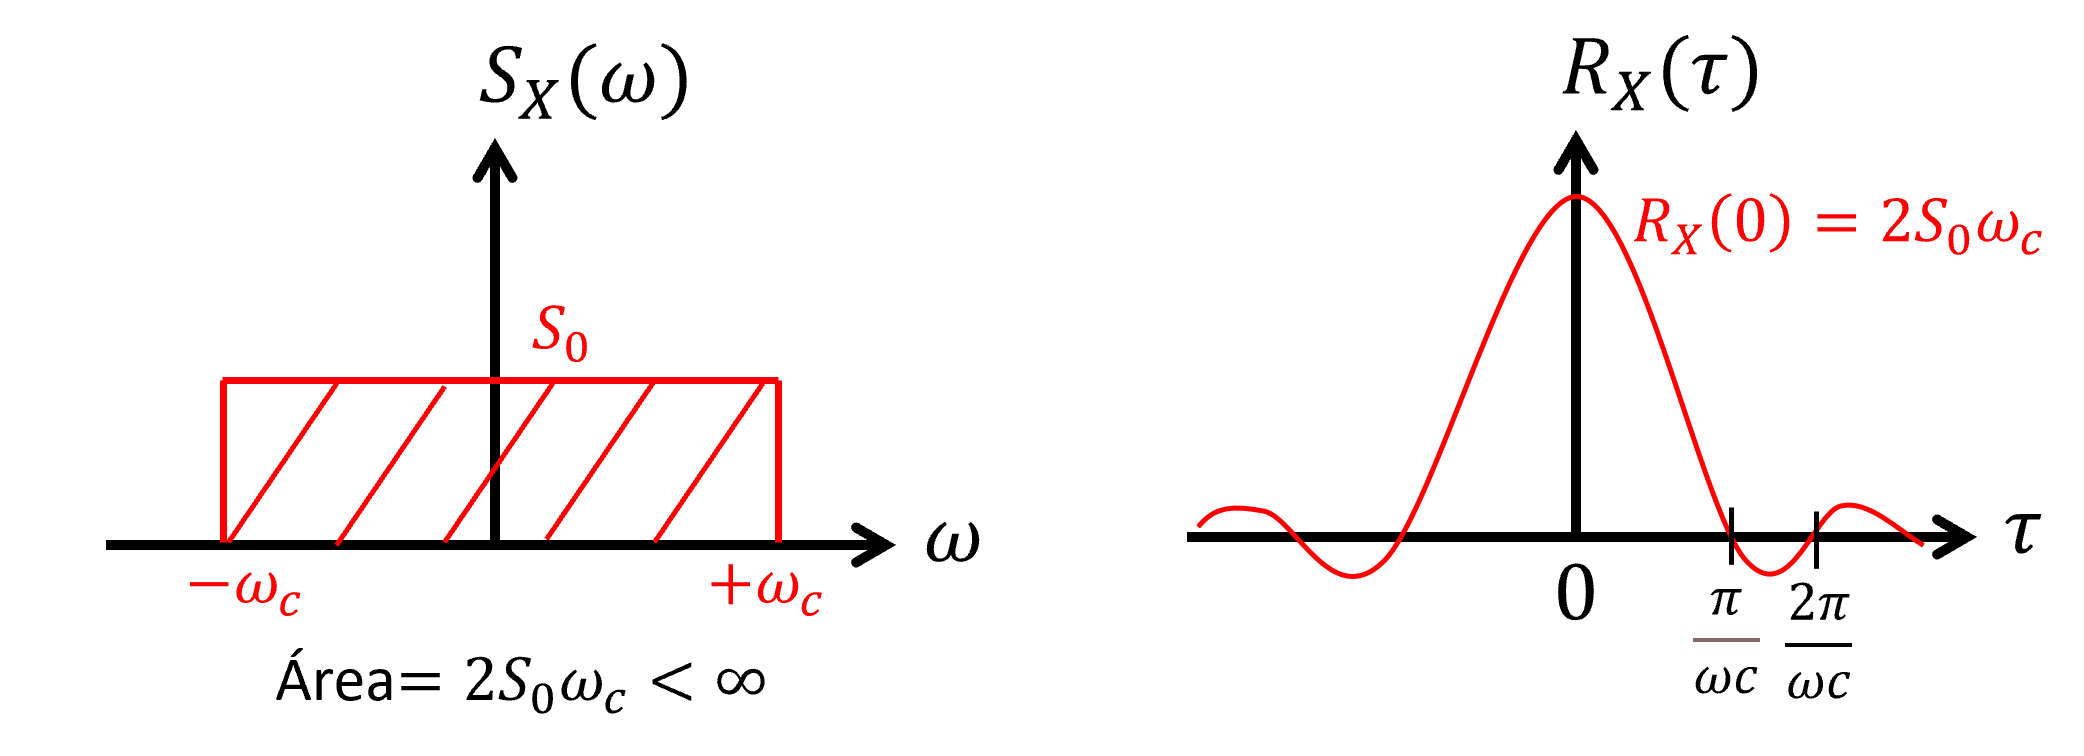
\includegraphics[scale=0.7]{Figuras/BLWN.png}
\end{figure}

Nota: a veces este p.e. se conoce como un filtro de paso bajo (``low-pass filter'').

\section{Ergocidad}
Sea $X=(X(t),t\in T)$ un p.e. estacionario, se dice que $X$ es ergódico si:
\begin{itemize}
    \item Ergódico en la media: 
    \begin{align*}
        \overline{\mu_X(t)}=\mu_X(t)
    \end{align*}
    \begin{itemize}
        \item $\overline{\mu_X(t)}$: media tiempo
        \item $\mu_X(t)$: media conjunto
    \end{itemize}
    \item Ergódico en el valor cuadrado:
    \begin{align*}
        \overline{\mathbb{E}\{X^2(t)\}} =\mathbb{E}\{X^2(t)\} 
    \end{align*}
    \begin{itemize}
        \item $\overline{\mathbb{E}\{X^2(t)\}}$: valor cuadrado tiempo
        \item $\mathbb{E}\{X^2(t)\}$: valor cuadrado conjunto
    \end{itemize}
    \item Ergódico en la correlación:
    \begin{align*}
        \overline{R_X(\tau)} = R_X(\tau)
    \end{align*}
    \begin{itemize}
        \item $\overline{R_X(\tau)}$: autocorrelación tiempo
        \item $R_X(\tau)$: autocorrelación conjunto
    \end{itemize}
\end{itemize}

Nota: Ruido blanco es un p.e. Gaussiano, y es ergódico.

\section{Respuesta estocástica de sistemas lineales}
Sea un sistema LTI, determinístico:
\begin{align*}
    \tend{\dot{x}} =\tenq{A}\tend{x}+\tenq{B}u, \quad x(0)=x_0=0
\end{align*}
y asuma que $u(t)$ es un p.e. w.s.s., $\mu_U=0$.
\par \underline{Objetivo}: Determinar la respuesta $x(t)$, p.e. w.s.s., $\mu_X=0$\\
\par Calculemos la autocovarianza de $\tend{x}(t)$
\begin{align*}
    \tenq{\Gamma}_X(t)=\mathbb{E}[XX^\top]=
\end{align*}

La derivada de $\tenq{\Gamma}_X(t)$:
\begin{align*}
    \frac{d}{dt}\tenq{\Gamma}_X(t)&=\frac{d}{dt}\mathbb{E}[XX^\top]=\mathbb{E}\bigl[\frac{d}{dt}(XX^\top)\bigr]\\
    &= \mathbb{E}[\dot{X}X^\top+X\dot{X}^\top]\\
    &= \mathbb{E}\Bigl[(AX+BU)X^\top+X(AX+BU)^\top\Bigr]\\
    &= A\mathbb{E}[XX^\top]+B\mathbb{E}[UX^\top]+\mathbb{E}[XX^\top]A^\top+\mathbb{E}[XU^\top]B^\top\\
    \dot{\Gamma}_X &= A\Gamma_X+\Gamma_XA^\top+Q \quad \text{Ecuación diferencial de Lyapunov}
\end{align*}


donde $Q=\mathbb{E}\{BUX^\top\}+\mathbb{E}\{XU^\top B^\top\}$\\

\par Si $u(t)$ es un ruido blanco: 
\begin{itemize}
    \item $\mu_U=0$
    \item $\mathbb{E}\{U(t)U(t+\tau)\}=2\pi s_o\delta (\tau)$, $S_u=S_0$, $\forall \omega$
\end{itemize}

\underline{Aparte}: La solución analítica de $x(t)$ es:

\begin{equation*}
    x(t)=\phi(t)x_0+\int_0^t \phi(t-\tau)Bu(\tau)d\tau
\end{equation*}

Desarrollemos el primer término de $Q$:
\begin{align*}
    \mathbb{E}\{BU(t)X^\top (t)\} &=  \mathbb{E}\{BU(t)[\int_0^t \phi(t-\tau)Bu(\tau)d\tau]^\top\}\\
    &= B\int_0^t \mathbb{E}\{U(t)[U^\top (t) B^\top \phi^\top (t-\tau)] \} d\tau\\
    &= B\int_0^t \mathbb{E}\{U(t)U^\top (t)\} B^\top \phi^\top (t-\tau) d\tau
\end{align*}

Dado que $U$ es un ruido blanco:
\begin{align*}
    \Longrightarrow \mathbb{E}\{U(t)U(t+\tau)=2\pi s_0 \delta (\tau)
\end{align*}

Pueden demostrar que:
\begin{align*}
    \mathbb{E}\{BUX^\top \}=\frac{1}{2}B2\phi s_0B^\top
\end{align*}

\begin{align*}
    Q &= \mathbb{E}\{BUX^\top \}+\mathbb{E}\{BU^\top X^\top \}=2\mathbb{E}\{BUX^\top \}\\
    Q &= B(2\pi s_0)B^\top
\end{align*}

Para resolver $\Gamma_X(t)$, se calcula $Q$ que depende de $s_0$:
\begin{align*}
    \dot{\Gamma}_X(t)=A\Gamma_X+\Gamma_XA^\top +Q
\end{align*}

La solución es única ssi A es Hurwitz.\\
\par \underline{Notas}:
\begin{itemize}
    \item $Q$ es una matriz simétrica, definida positiva. Entonces, $s_0$ es una matriz simétrica, definida positiva.
    \item $\Gamma_X$ es una matriz simétrica, definida positiva.
\end{itemize}

Veamos qué ocurre en estado estacionario ($t\to \infty$)
\begin{align*}
    \lim_{t\top \infty} \dot{\Gamma}_X(t)=0
\end{align*}
Ecuación de Lyapunov:
\begin{align*}
   0=A\Gamma_X+\Gamma_XA^\top +Q
\end{align*}

Solución: $\Gamma_X$, autocovarianza estacionaria de $X(t)$.\\

\par Dada la ec. de respuesta:
\begin{align*}
    y(t) = Cx(t)
\end{align*}
donde $y(t)$ es un p.e., w.s.s., $\mu_y=0$.\\
\par Matriz autocovarianza respuesta:
\begin{align*}
    \Gamma_Y=\mathbb{E}\{YY^\top\} &= \mathbb{E}\{(CX)(CX)^\top\}\\
     &= \mathbb{E}\{CXX^\top C^\top\}\\
      &= C \mathbb{E}\{XX^\top\}C^\top\\
       &= C \Gamma_X C^\top\\
\end{align*}



\section{Modelos de Carga Estructural Estocástica}
Una gran cantidad de excitación sobre sistemas estructurales son estocásticos por naturaleza.\\
\par Ejemplos:
\begin{itemize}
    \item Terremotos
    \item Viento
    \item Tránsito vehicular
    \item Rugosidad pavimento
    \item Oleaje
\end{itemize}

Para cada uno de estos tipos de excitación, se puede formular un modelo que captura las principales características de la carga estocástica en cuestión:
\begin{itemize}
    \item Carga sísmica: 
    \begin{itemize}
        \item Kanai-Tajimi
        \item Clough-Penzien
        \item Etc.
    \end{itemize}
    \item Carga viento:
    \begin{itemize}
        \item Daurenport
        \item Kaimal \& Vonkerman
        \item Etc.
    \end{itemize}
    \item Oleaje:
    \begin{itemize}
        \item Pierson-Moskowitz
        \item Etc.
    \end{itemize}
\end{itemize}

\section{Modelo Kanai-Tajimi}
El modelo K-T genera un p.e. Gaussiano estacionario, que representa la aceleración del suelo producto de un evento sísmico: \\

\begin{figure}[H]
\centering
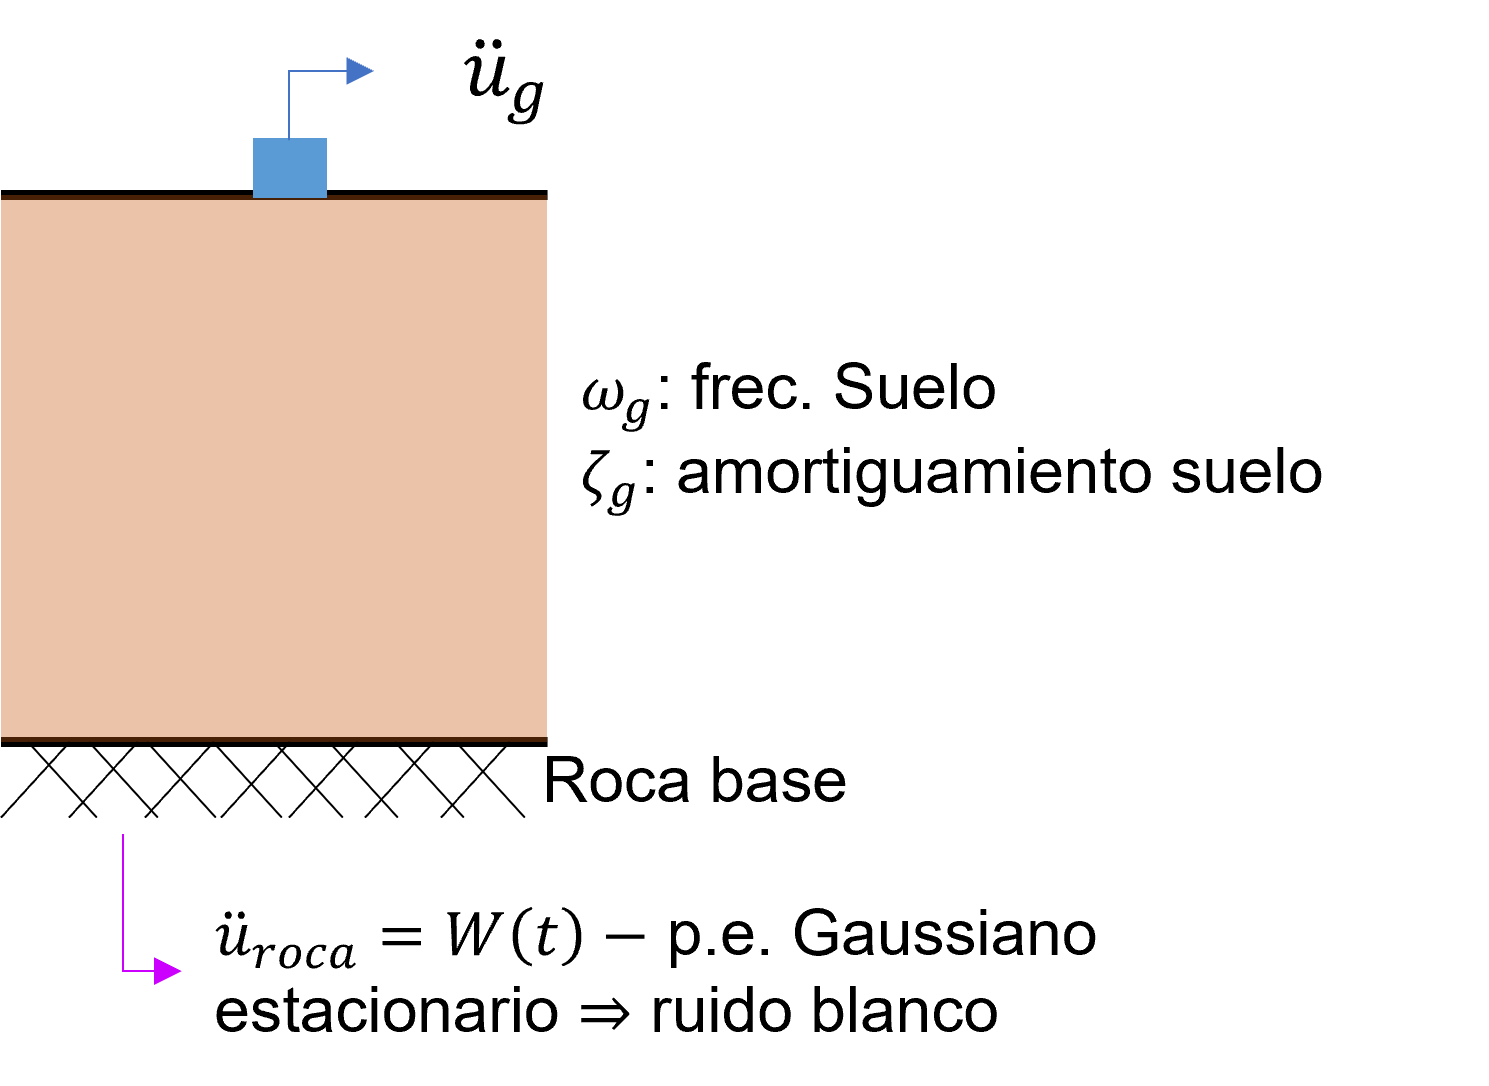
\includegraphics[scale=0.7]{Figuras/KT.png}
\end{figure}
EDM: $a$- estado del suelo
\begin{align*}
    \ddot{a}+2\xi_g\omega_g\dot{a}+\omega_g^2a=W(t) 
\end{align*}

Ruido blanco: 
$$\mathbb{E}\{W(t)\}=0$$ 
$$\mathbb{E}\{W(t)W(t+\tau)\}=2\pi S_0\delta(\tau)$$

$S_0$: poder espectral del sismo en roca (Intensidad del terremoto).\\

\par Ecuación de respuesta:
\begin{align*}
    \ddot{u}_g = -2\xi_g\omega_g \dot{a}-\omega_g^2a
\end{align*}
donde $\ddot{u}_g$ es la aceleración del suelo en campo libre.\\
\par Se puede demostrar que la función de respuesta en frecuencia (FRF) del estado de suelo es:

\begin{align*}
    H_{KT}(\Omega) &= \frac{\omega_g^2+i2\xi_g\omega_g\Omega}{(\omega_g^2-\Omega^2)+i2\xi_g\omega_g\Omega}\\
    |H_{KT}(\Omega)| &= \frac{\omega_g^4+4\xi_g^2\omega_g^2\Omega^2}{(\omega_g^2-\Omega^2)+4\xi_g^2\omega_g^2\Omega^2}
\end{align*}

\begin{figure}[H]
\centering
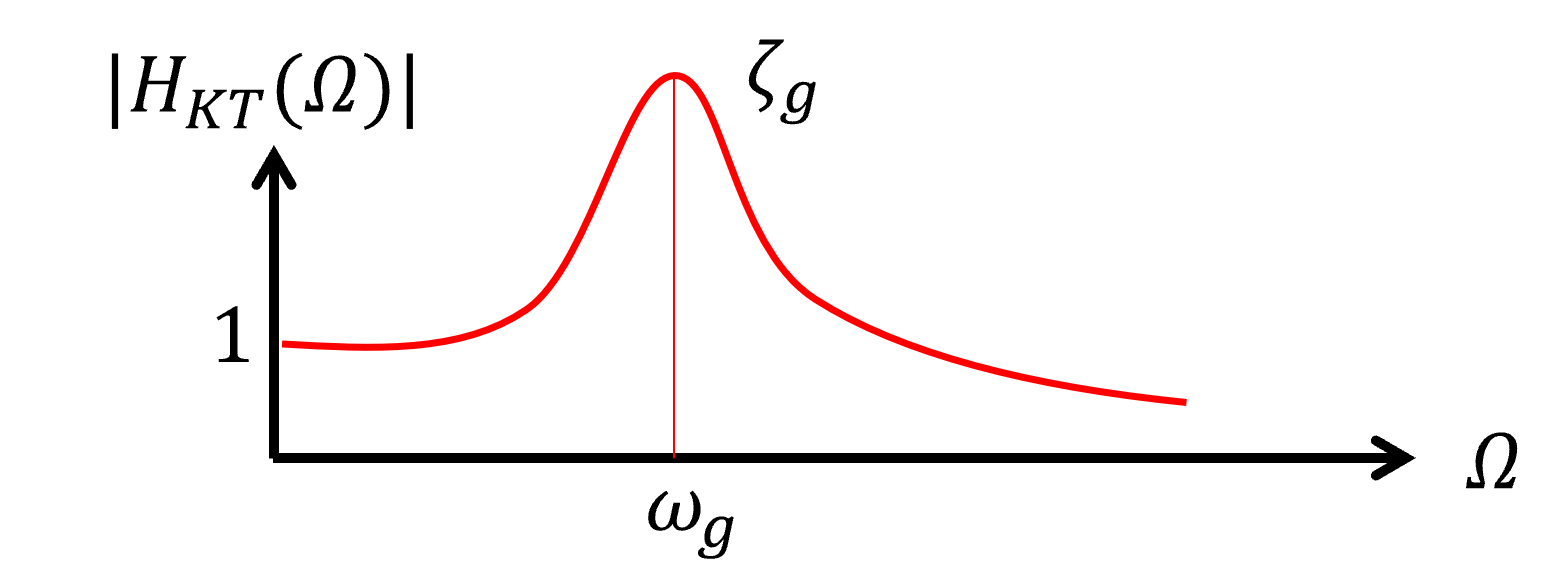
\includegraphics[scale=0.7]{Figuras/HKT.png}
\end{figure}


En espacio-estado:
\begin{align*}
    \dot{x}_g &= A_gx_g+B_gw(t), \quad x_g=a\\
    y_g &= C_gx_g, \quad y_g=\ddot{u}_g
\end{align*}

Diagrama de bloques:

\begin{figure}[H]
\centering
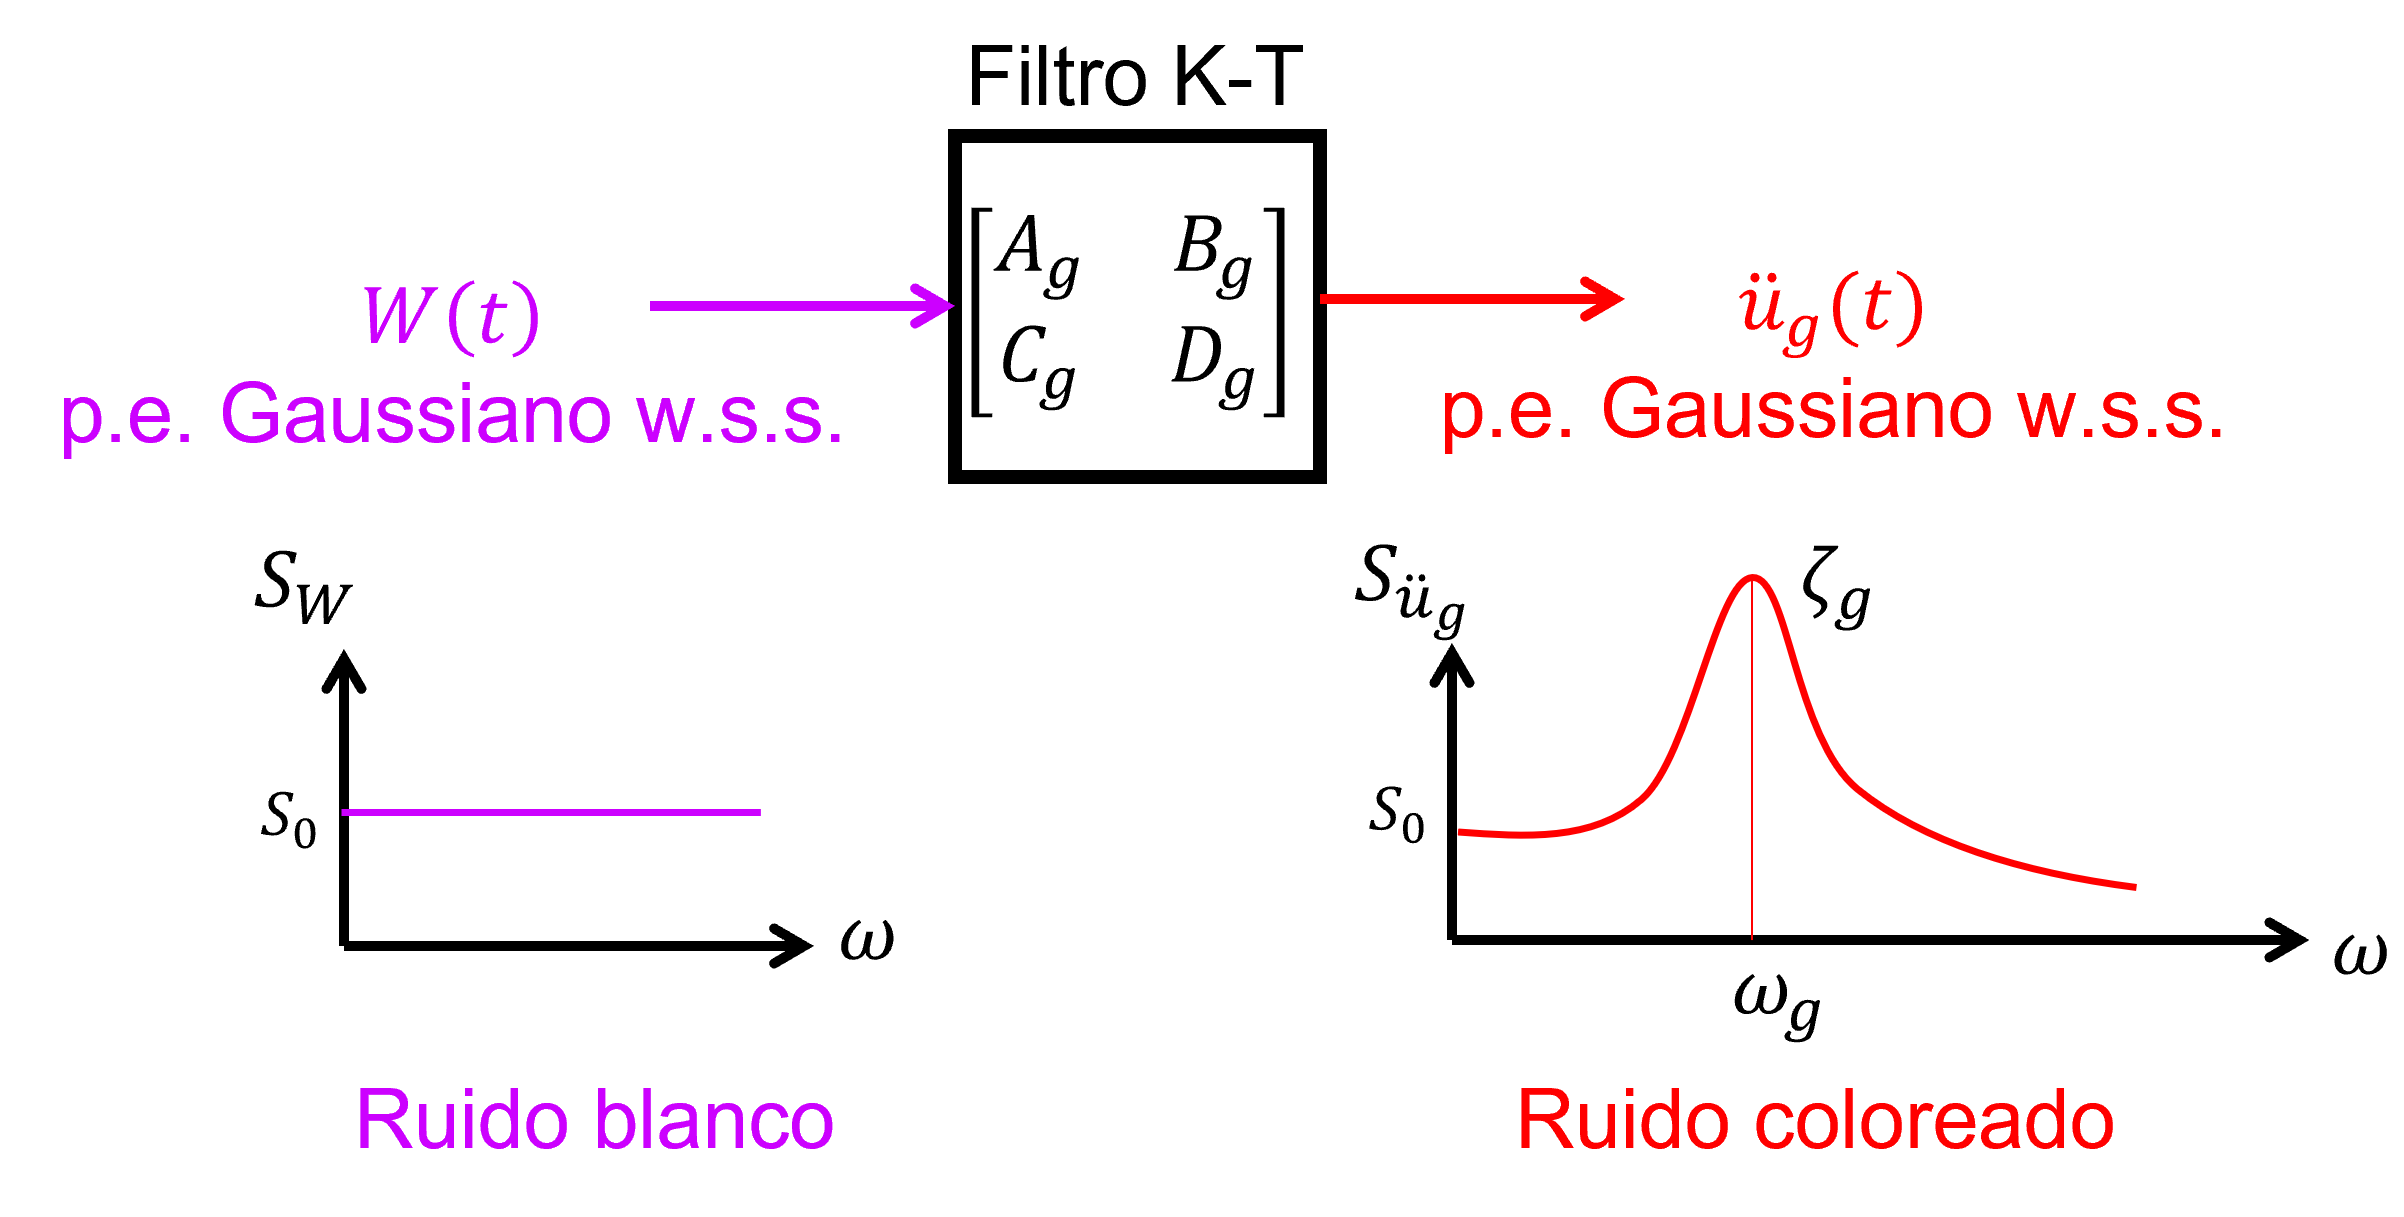
\includegraphics[scale=0.6]{Figuras/diagrama_bloque_KT.png}
\end{figure}

\begin{align*}
    \ddot{u}_g(t) &= h_{KT} \ast W(t)\\
    \ddot{u}_g(t)\ddot{u}_g(t+\tau) &= h_{KT}^2(t) \ast W(t)W(t+\tau)\\
    \Longrightarrow s_{\ddot{u}_g}(\omega) &= |H_{KT}(\omega)|^2s_0
\end{align*}

Parámetros del modelo K-T: $s_0$, $\omega_g$, $\xi_g$.\\
\par Terremoto El Centro (1940): 
\begin{itemize}
    \item $\bar{\omega}_g = 18$ rad/s
    \item $\bar{\xi}_g = 0.60$
    \item $s_0 = $ depende del peak ground acceleration (PGA)
\end{itemize}

En estado estacionario:

\begin{figure}[H]
\centering
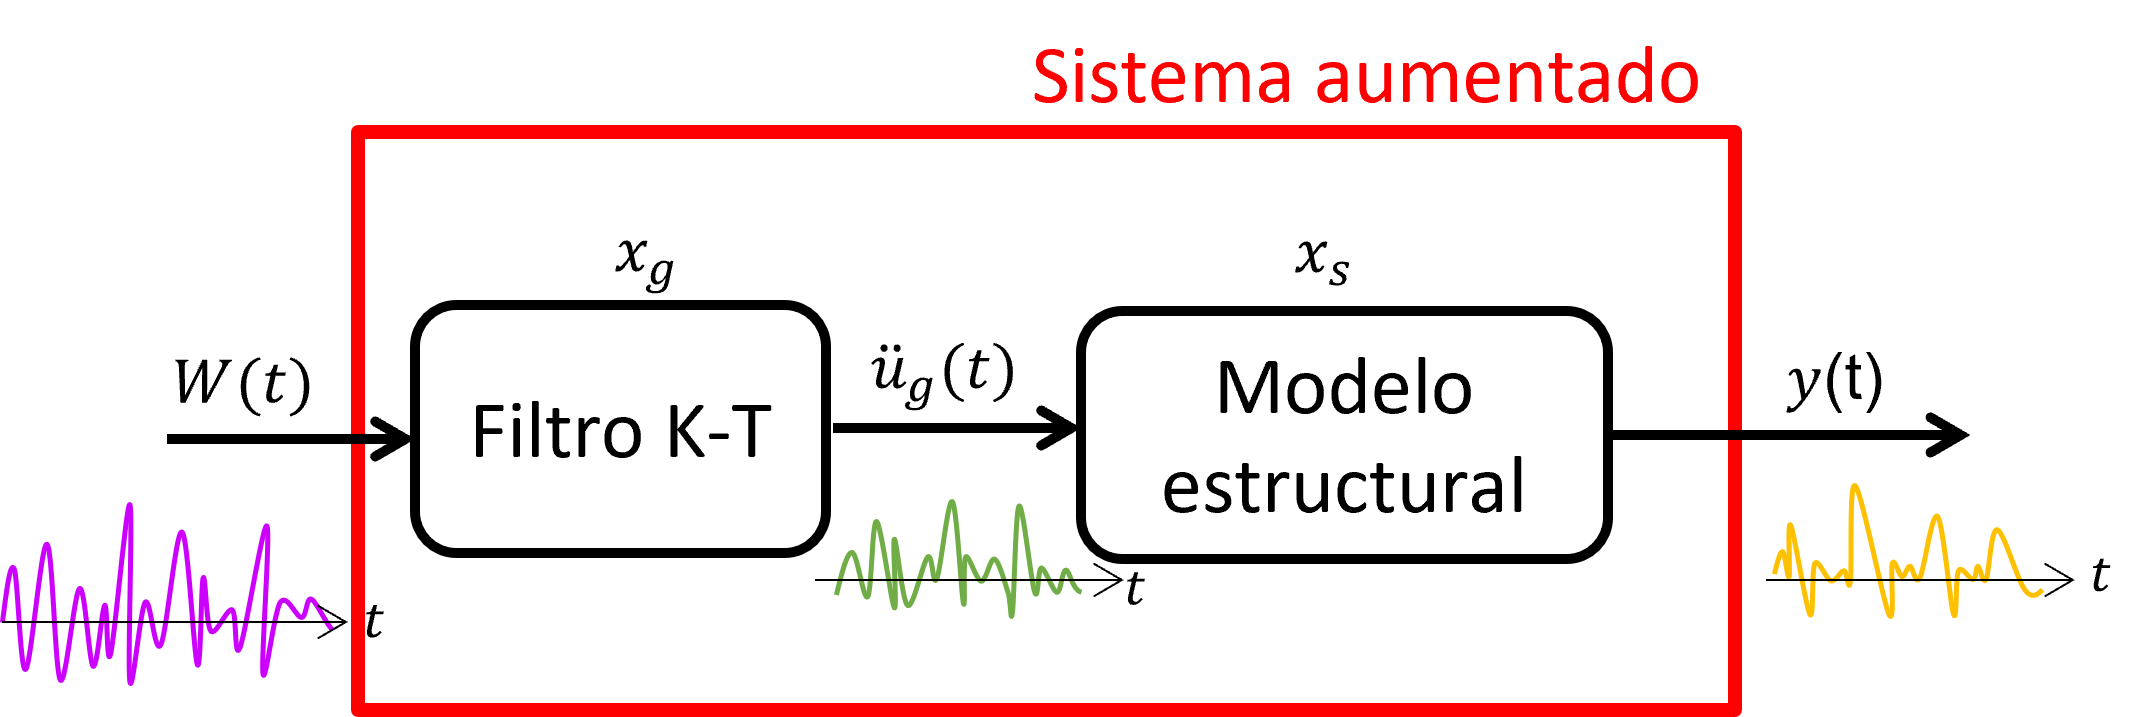
\includegraphics[scale=0.7]{Figuras/estado_estacionario_KT.png}
\end{figure}
Estados: $x_a=\left\{
    \begin{array}{c}
     x_s \\ x_g 
    \end{array}\right\}$
\begin{align*}
    \dot{x}_a&=A_ax_a+B_aW(t)\\
    y &= C_ax_a
\end{align*}

\par Ec. de Lyapunov:
\begin{align*}
    0 &= A_x\Gamma_x +\Gamma_aA_a^\top+Q_a\\
    \Gamma_a &= \mathbb{E}\{x_ax_a^\top\}\\
    \Gamma_y &= C_a\Gamma_aC_a^\top \Longrightarrow \text{RMS respuesta}
\end{align*}

Pero, en realidad los registros sísmicos son p.e. no estacionarios:

\par ¿Podemos ocupar K-T? $\longrightarrow$ Sí, a través de una \textcolor{red}{función de modulación}\\

\begin{figure}[H]
\centering
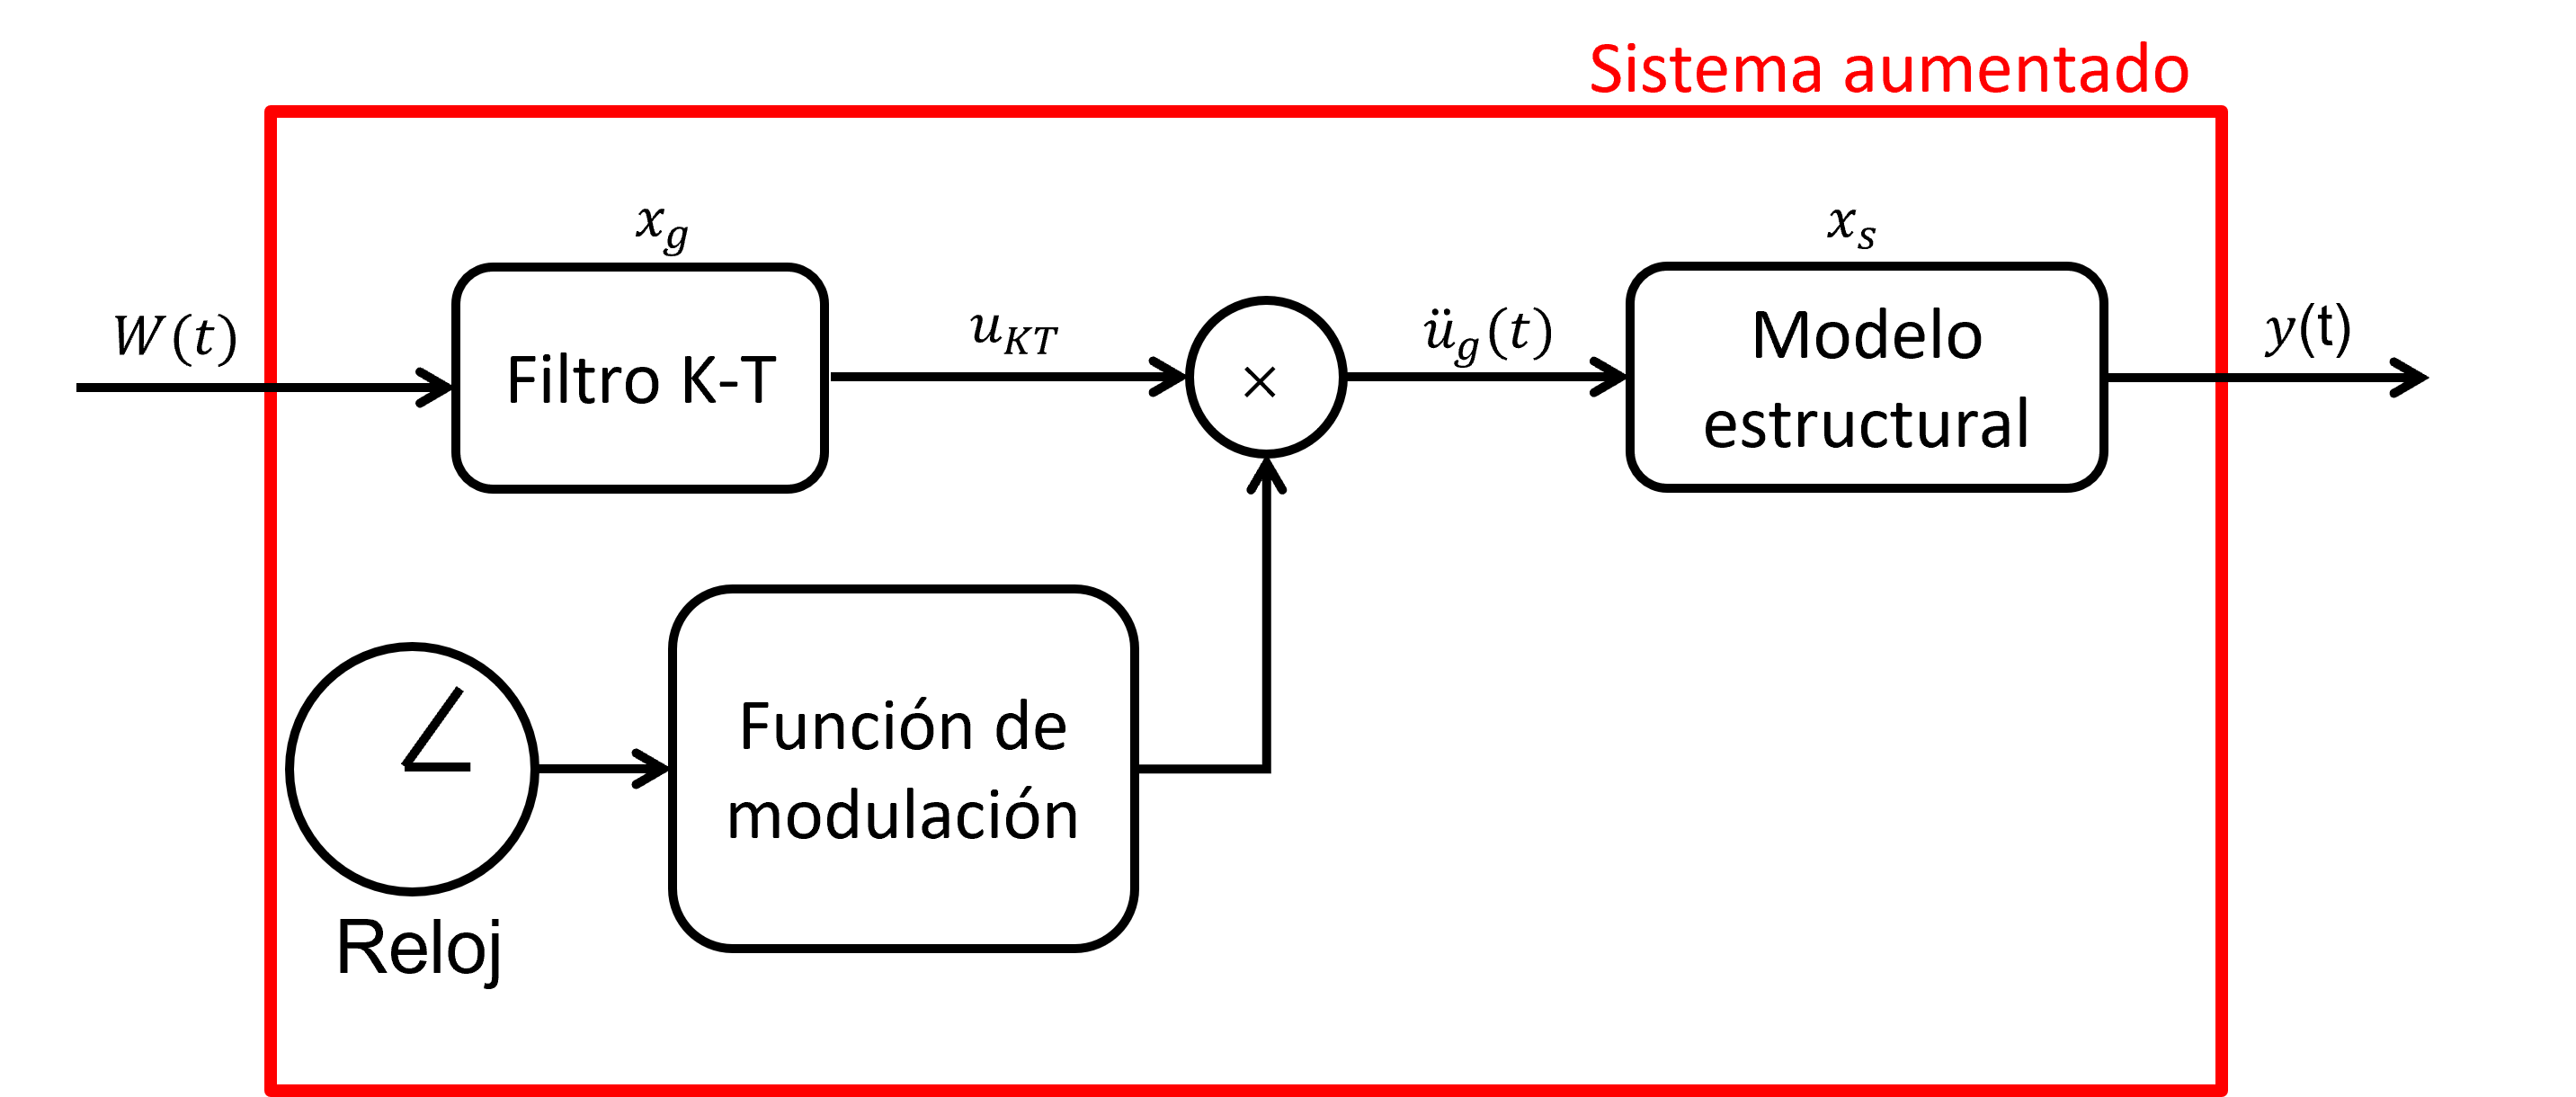
\includegraphics[scale=0.6]{Figuras/func_mod_KT.png}
\end{figure}
\begin{figure}[H]
\centering
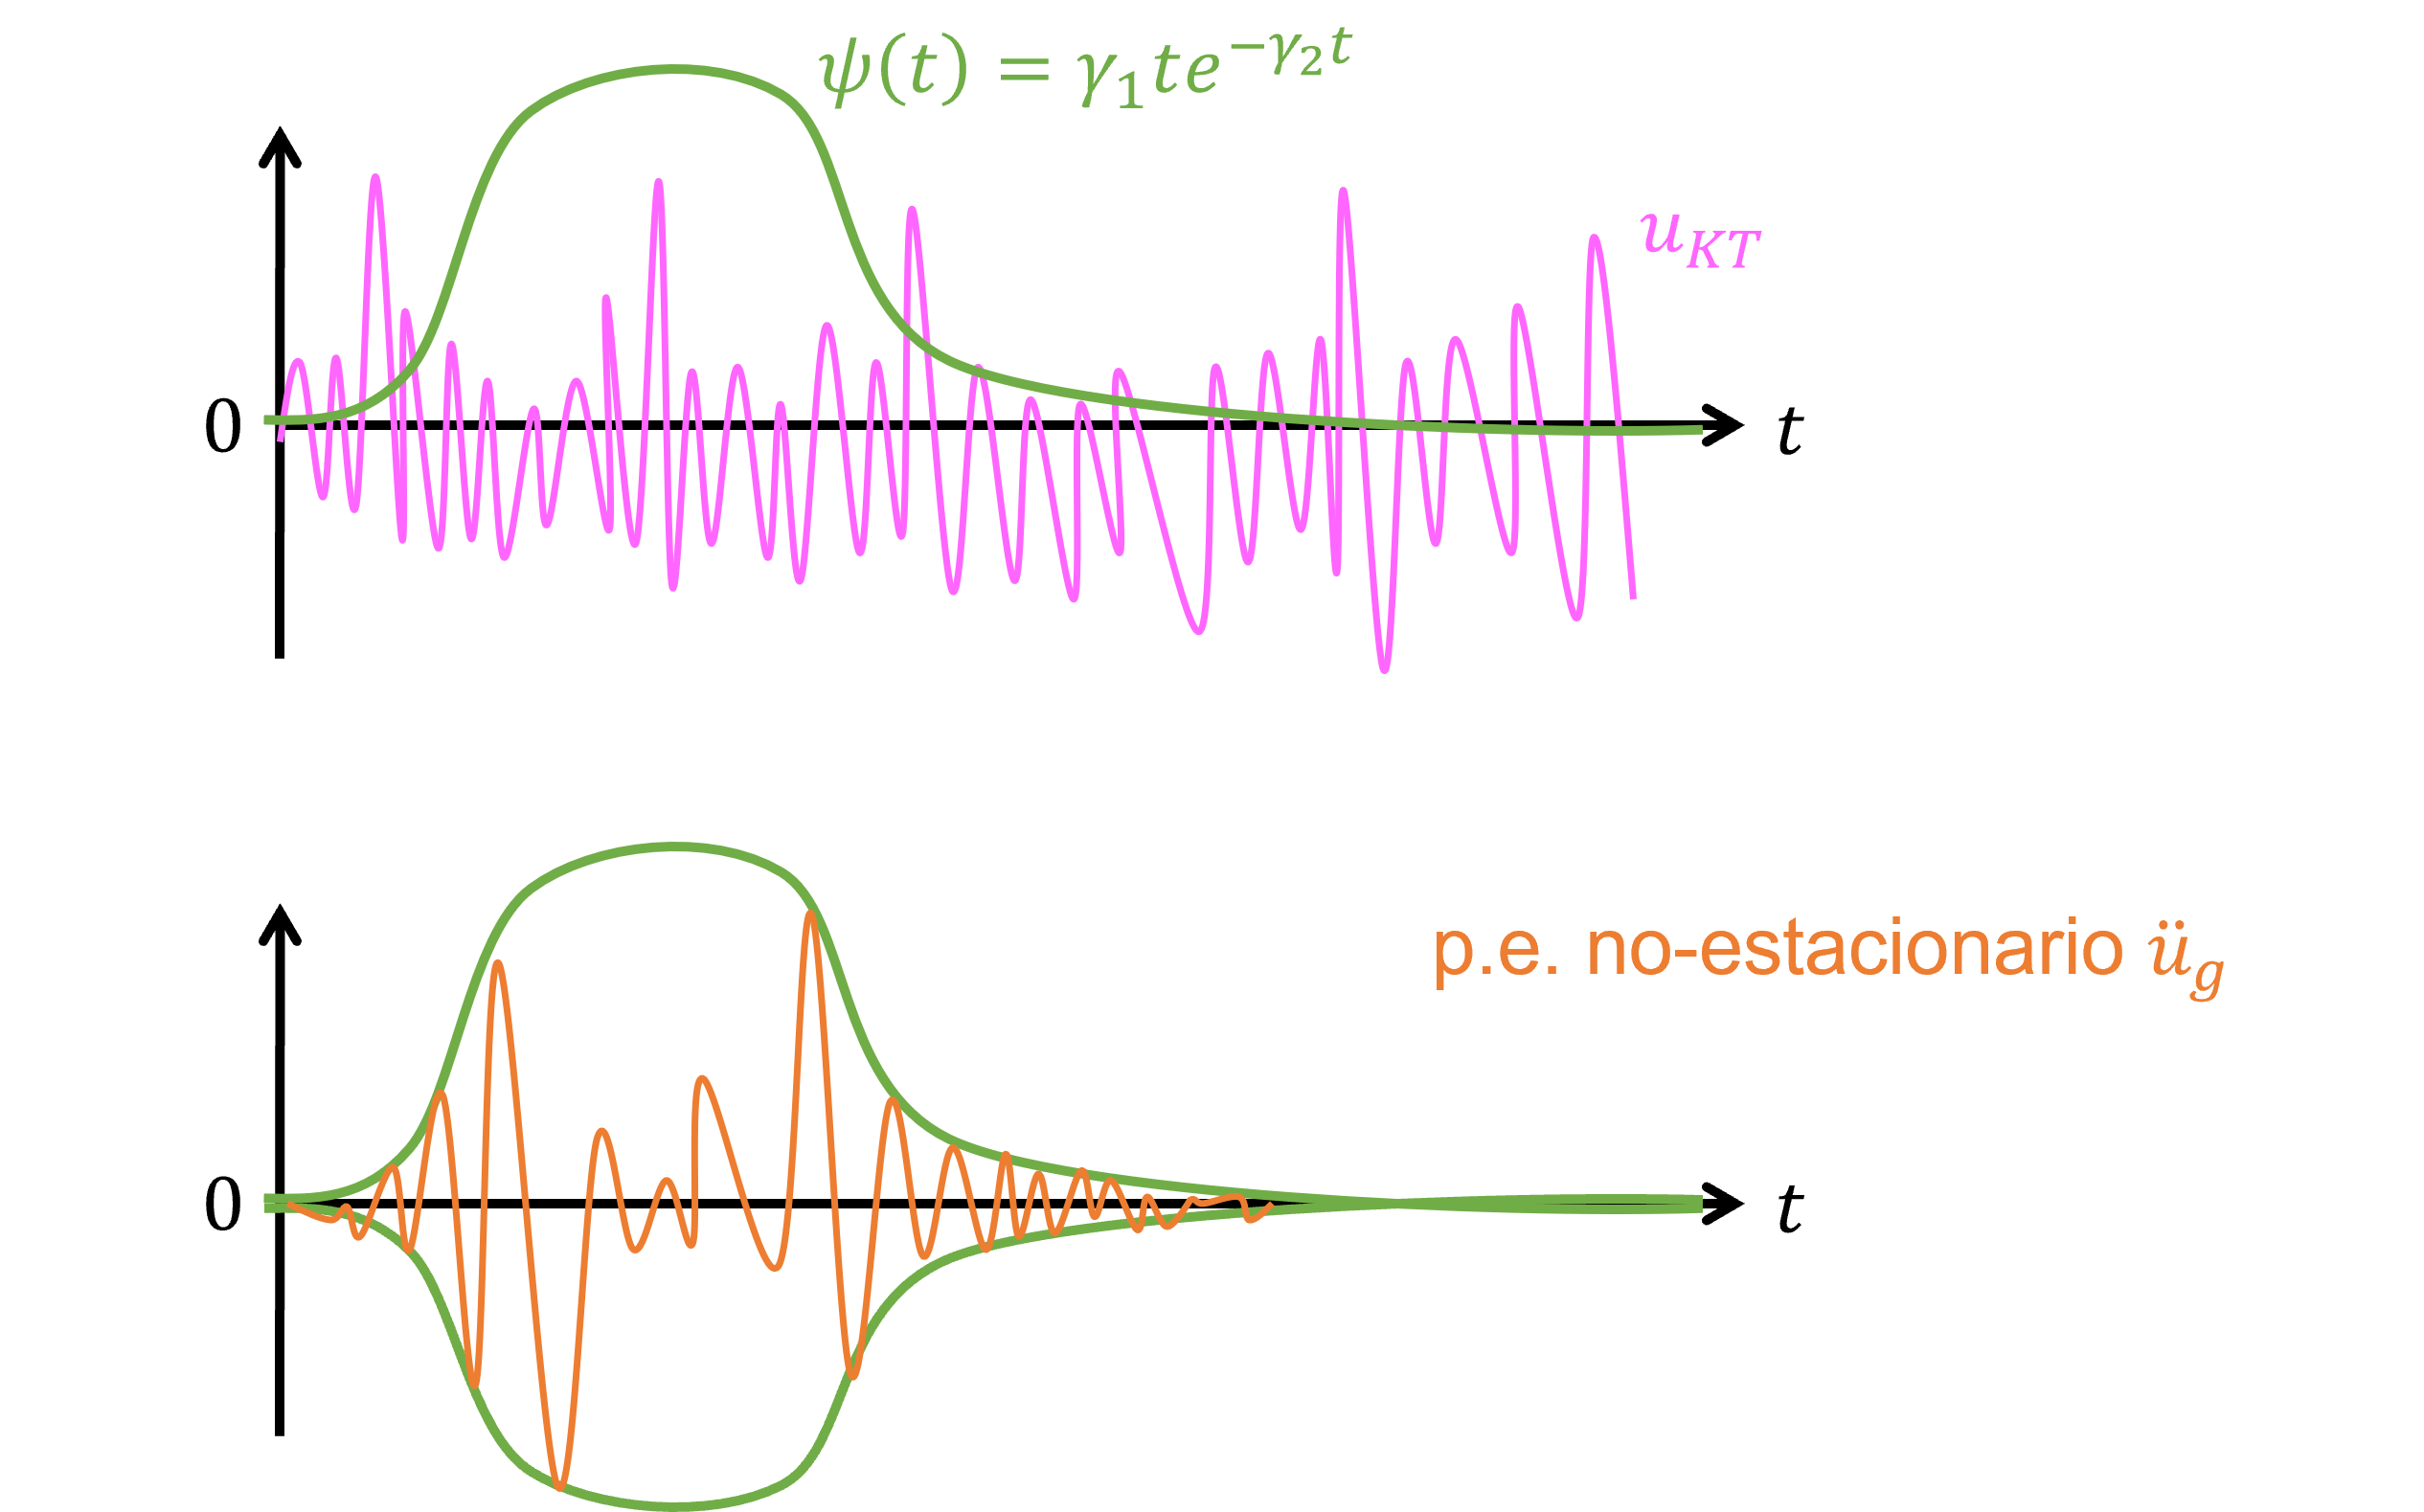
\includegraphics[scale=0.6]{Figuras/func_mod_KT2.png}
\end{figure}

\par Sistema atenuado (LTV): 
\begin{align*}
    \dot{x}_a(t) &= A_a(T)x_a(t)+B_a(t)Z(t)\\
    y(t) &= C_a(t)x_a(t)
\end{align*}
$\Longrightarrow$ Ec. diferencial de Lyapunov:
\begin{align*}
    \dot{\Gamma}_a(t) = A_a(t)\Gamma_a(t)+\Gamma_a(t)A_a^\top (t))+Q_a(t)
\end{align*}

Integrar, resolver $\Gamma_a(T)\Longrightarrow \Gamma_y (t) \Longrightarrow\text{rms } y(t)$.




%----------- Cap6 -----------%
\input{Capitulos/Identificación_sistemas}

%----------- Cap7 -----------%
\chapter{Procesamiento Digital de Señales}


\section{Sistemas discretos}
\begin{figure}[H]
\centering
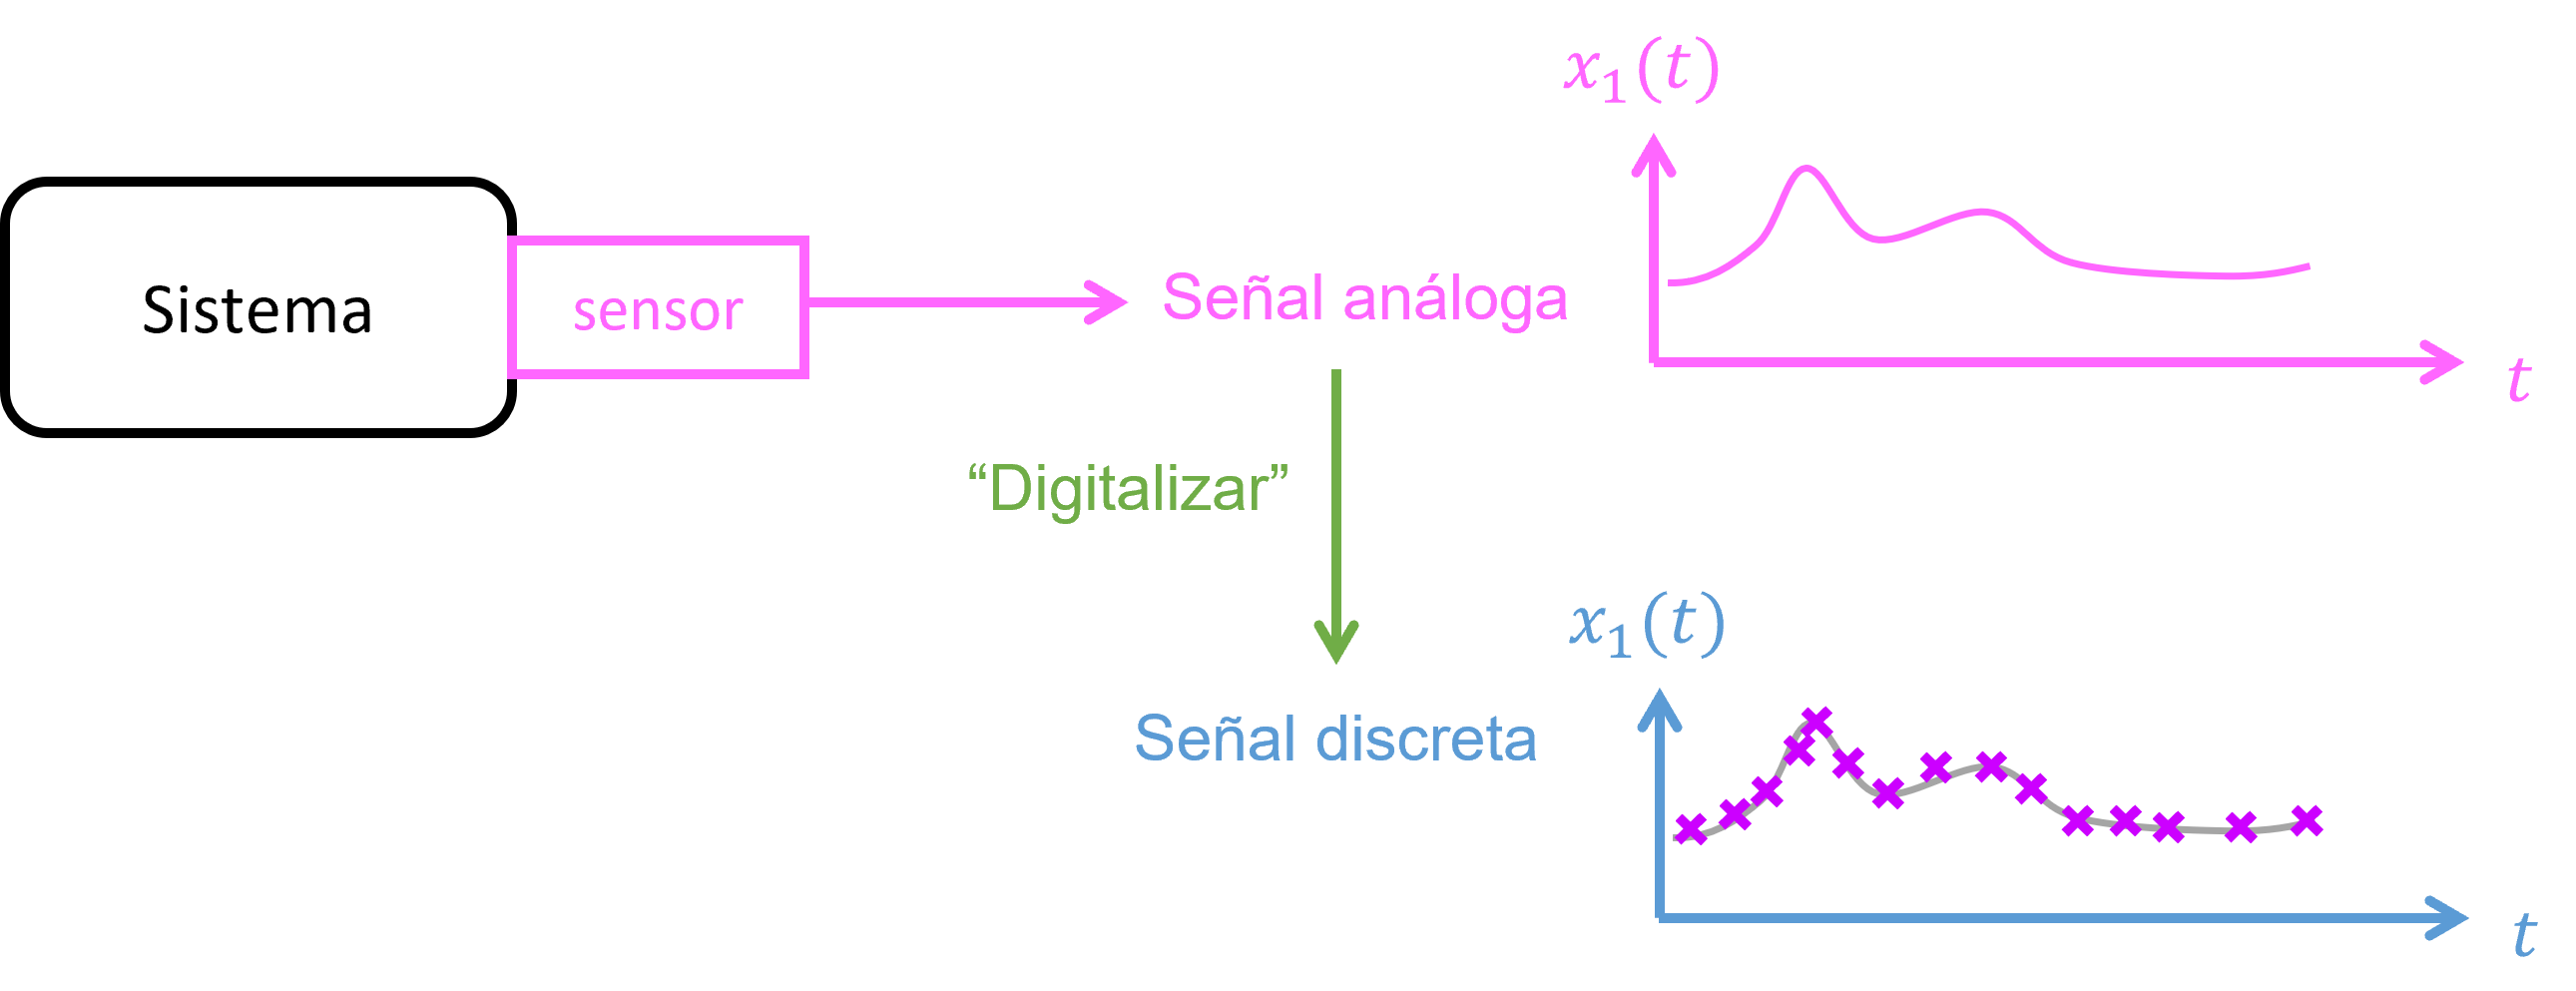
\includegraphics[scale=0.7]{Figuras/sist_discreto.png}
\end{figure}
\underline{Nota}: Computadores representan números utilizando dígitos binarios (bits, flip-flops). Es necesario convertir una señal análoga a discreta.\\

\par \underline{Muestreo (sampling)}: 
\begin{enumerate}
    \item Muestreo en el tiempo $\Longrightarrow$ Sampling
    \item Muestreo en amplitud $\Longrightarrow$ Quantization
\end{enumerate}

Máquina 16 bits $\Longrightarrow$ Números utilizando $2^{16}$ cifras significativas.
\begin{align*}
    \text{Bit} = \left\{ \begin{array}{l}
             0 \\
             1
             \end{array}
   \right. \Longrightarrow 65536 \text{ cifras significativas}
\end{align*}

\par \underline{Sistema discreto}:\\
\begin{figure}[H]
\centering
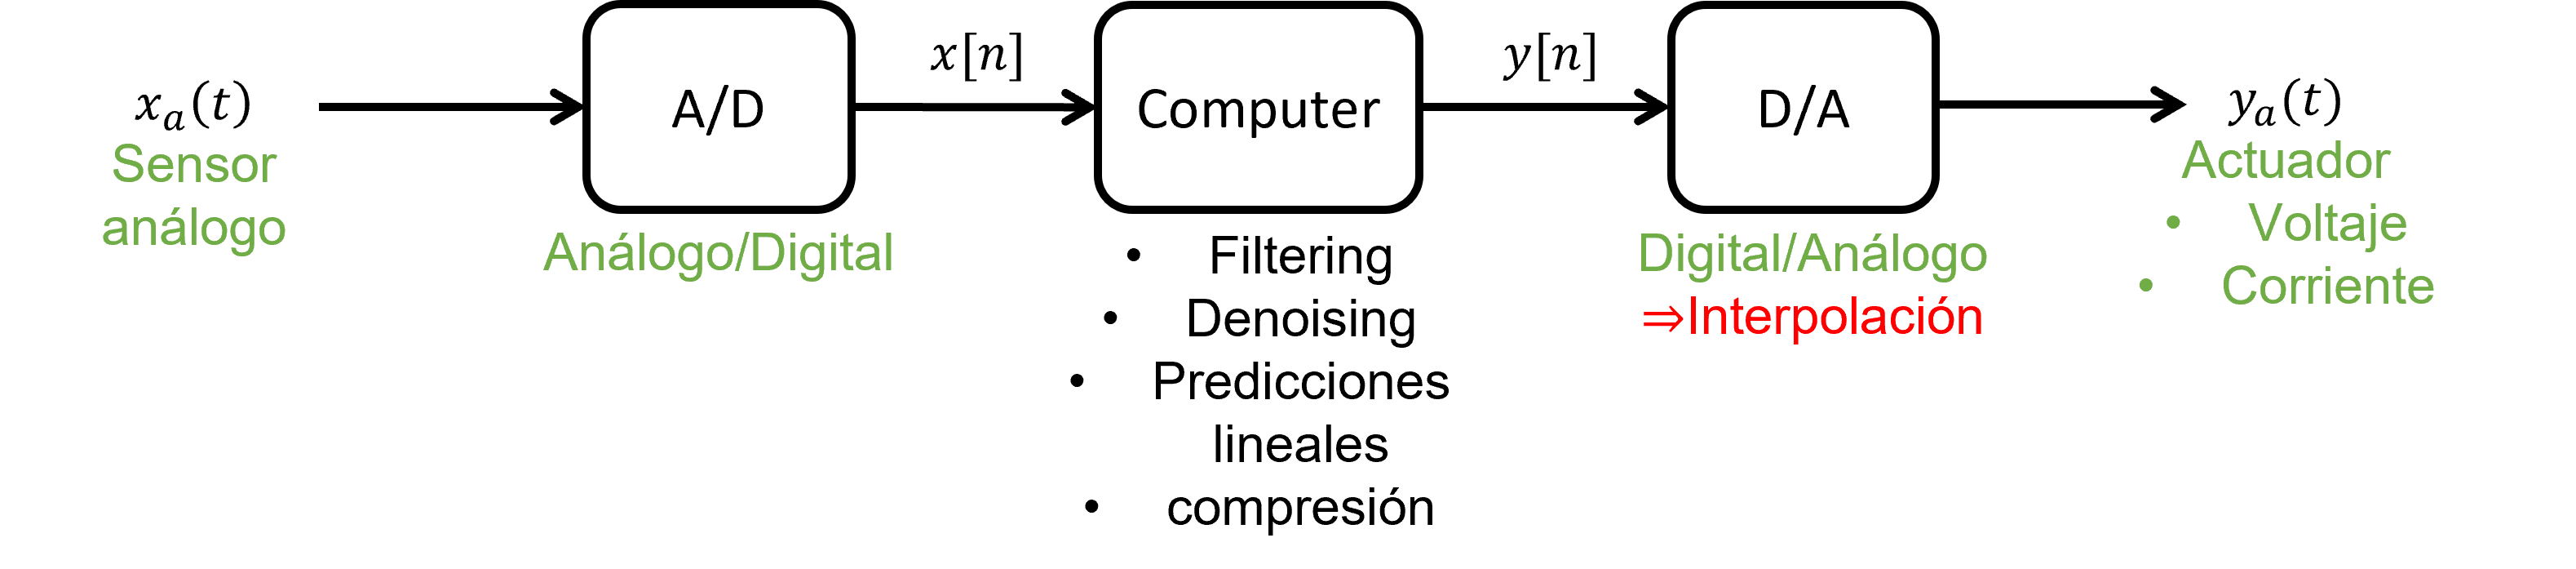
\includegraphics[scale=0.7]{Figuras/sistema_discret.png}
\end{figure}

$x[n]$: señal en tiempo discreto.\\
$$x[n]=x_a(nT)$$
T: intervalo de muestreo, n: índice (número entero)\\

\begin{figure}[H]
\centering
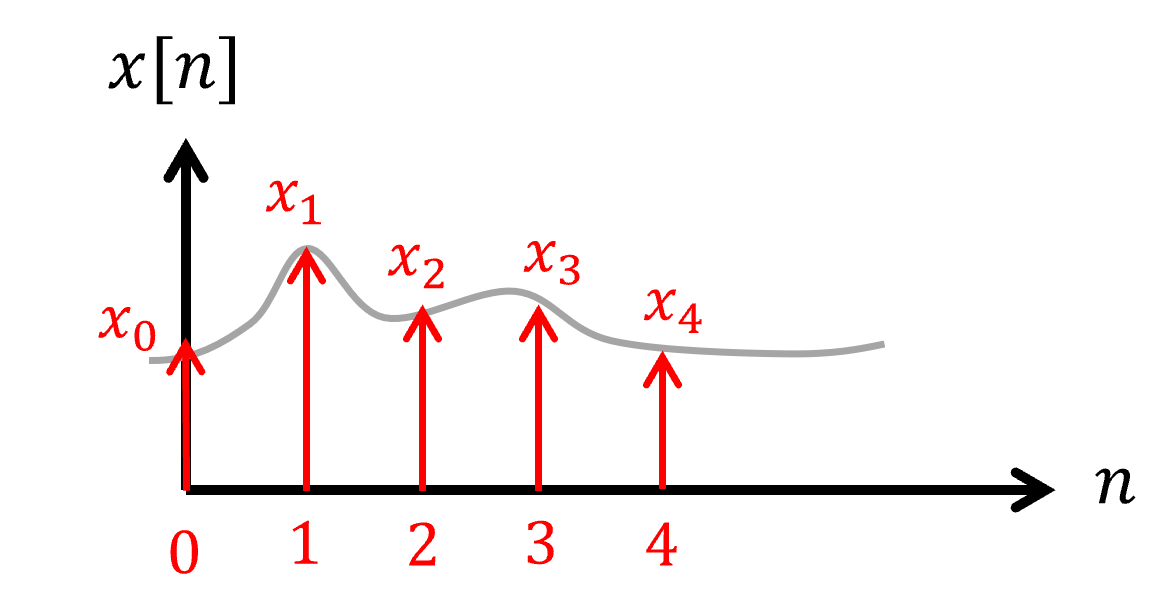
\includegraphics[scale=0.7]{Figuras/xn.png}
\end{figure}

\par \underline{Función pulso unitario}:
\begin{figure}[H]
\centering
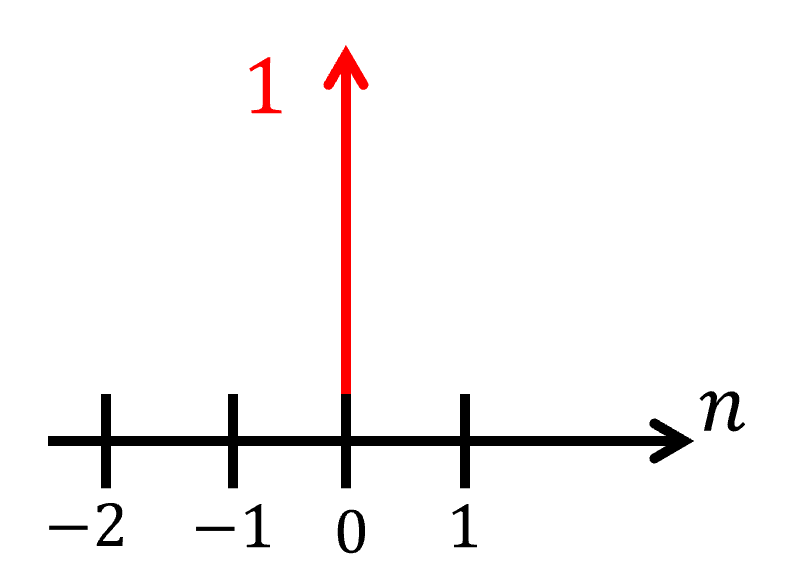
\includegraphics[scale=0.7]{Figuras/pulso_unitario.png}
\end{figure}
\begin{align*}
    \delta[n] = \left\{ \begin{array}{ll}
             1 & n=0\\
             1 & \text{else}
             \end{array}
   \right. 
\end{align*}

\begin{align*}
    x[n]=\sum_{k=0}^{N-1} x_k \delta[n-k]=x_0\delta[n]+x_1\delta[n-1]+x_2\delta[n-2]+...+x_{N-1}\delta[n-(N-1)]
\end{align*}

\begin{align*}
    \{x_n\}_0^{N-1}=\{x_0,x_1,x_2,...,x_{N-1}\} \Longrightarrow \text{Vector de N puntos}
\end{align*}
\begin{figure}[H]
\centering
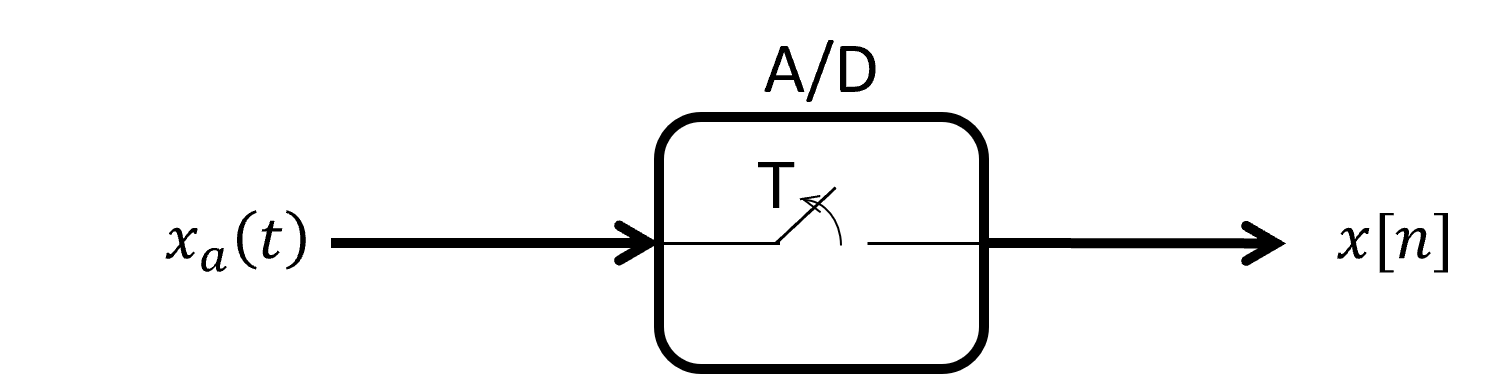
\includegraphics[scale=0.7]{Figuras/AD.png}
\end{figure}


\section{Análisis en frecuencia}
\begin{figure}[H]
\centering
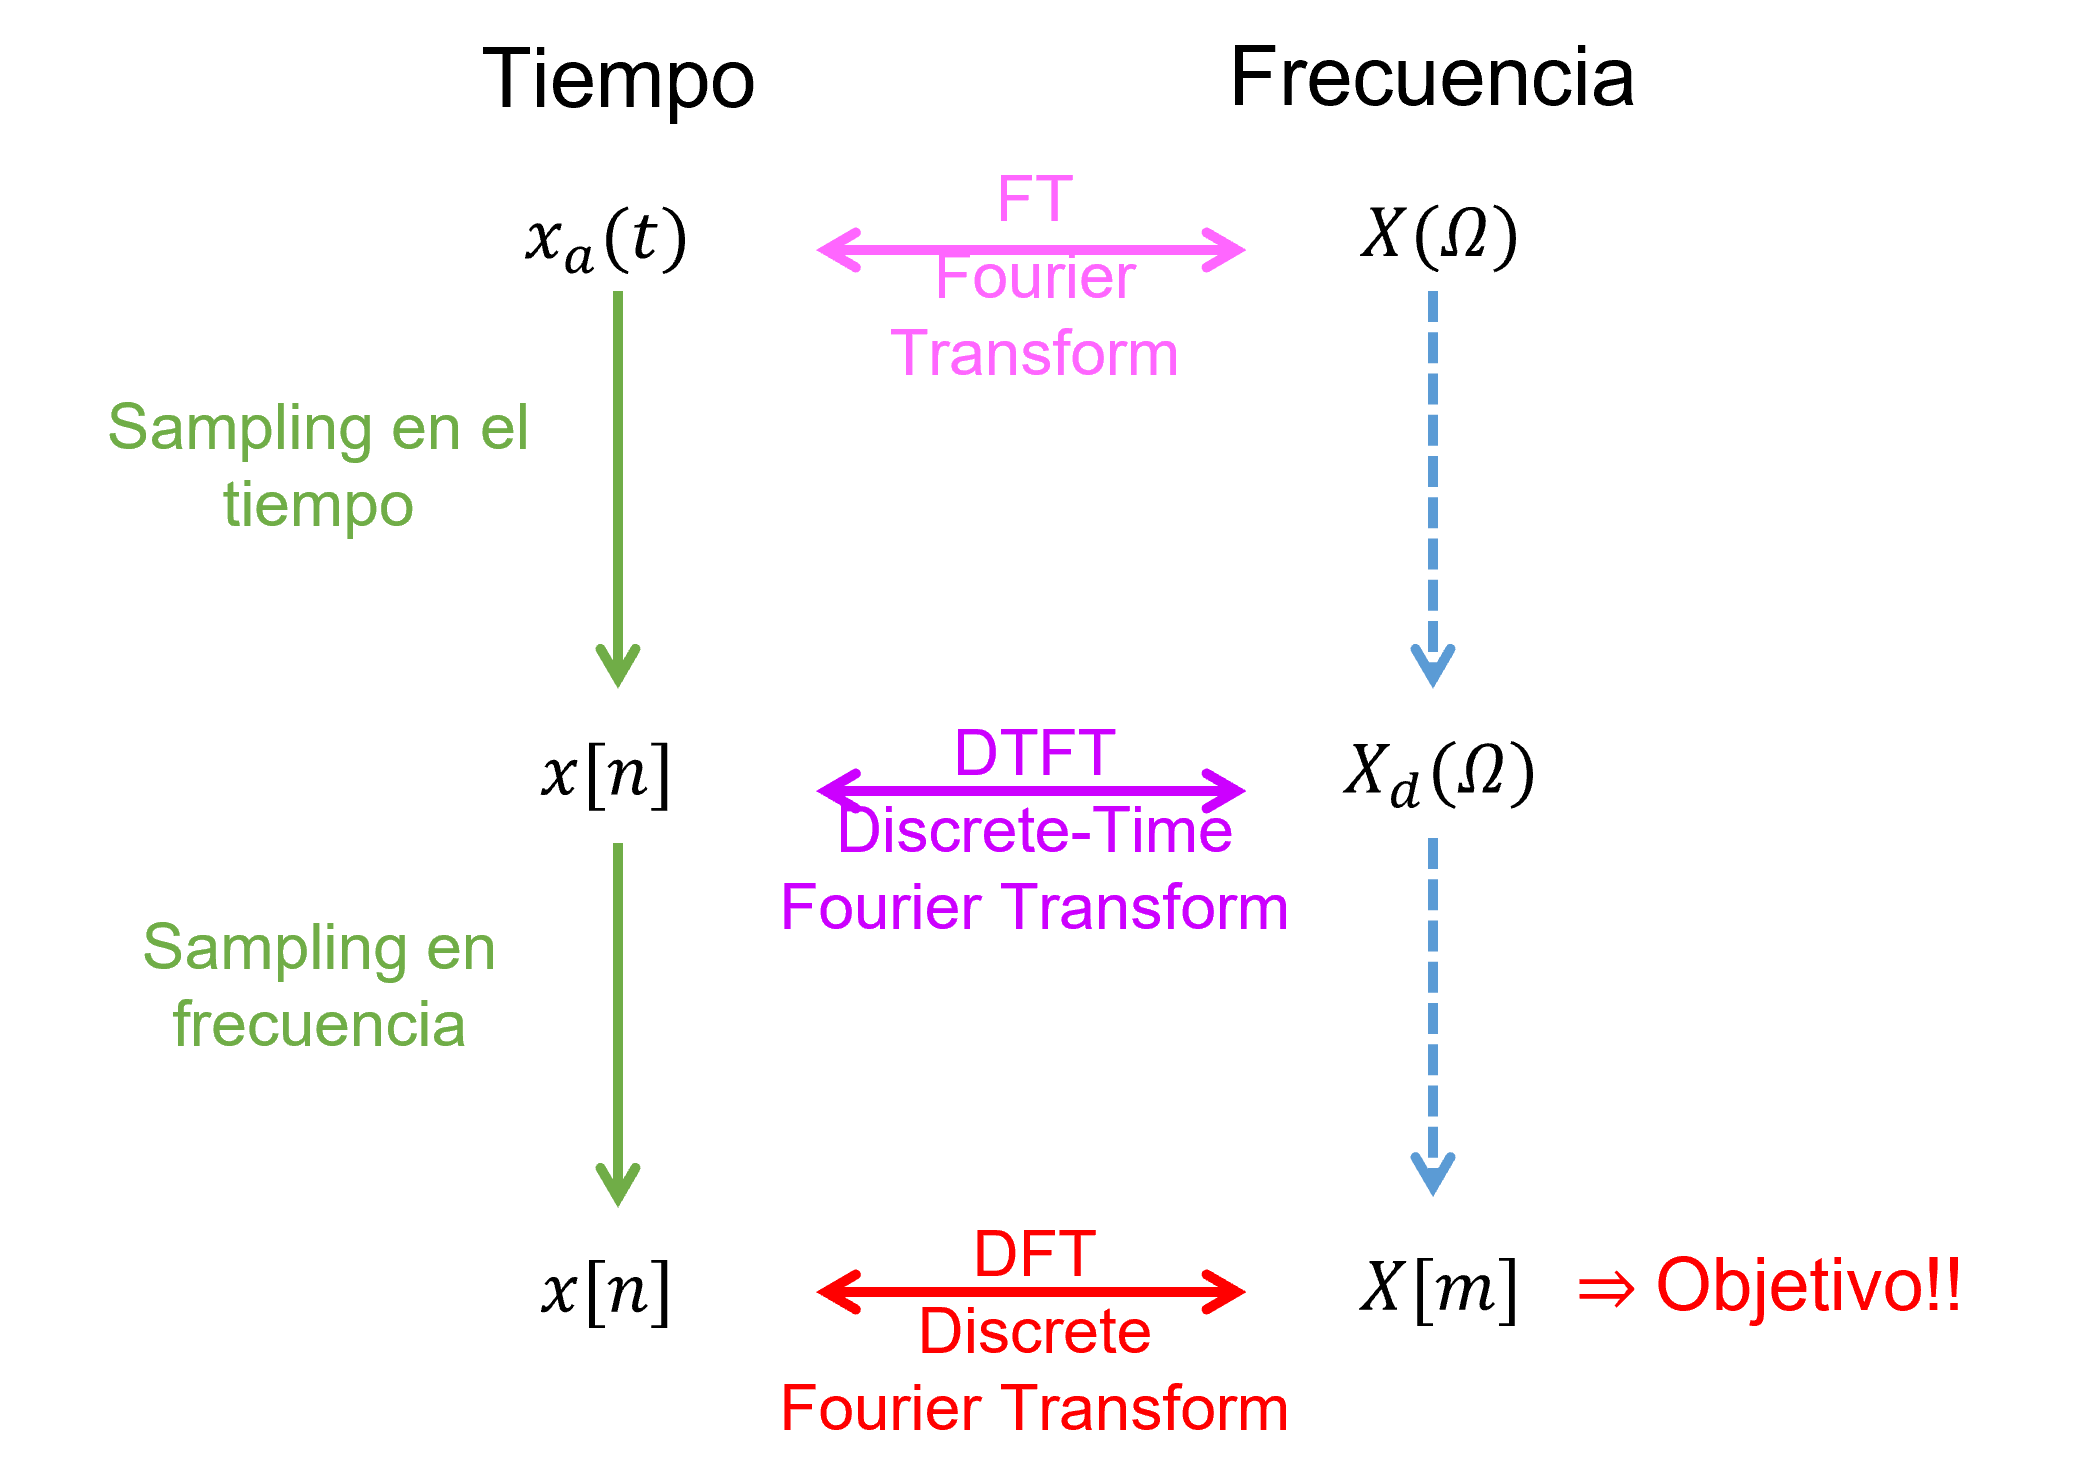
\includegraphics[scale=0.7]{Figuras/analisis_frec.png}
\end{figure}
\par \underline{Fourier Transform (FT)}
\begin{align*}
    X(\Omega) &= \int_{-\infty}^{+\infty}x_a(t)e^{-j\Omega t}dt \quad \text{(FT)}\\
    x_a(t) &= \frac{1}{2\pi}\int_{-\infty}^{+\infty}X(\omega)e^{+j\Omega t}d\Omega \quad \text{(inverse FT)}
\end{align*}

\underline{Nota}: $x_a(t)\in \mathbb{R}$, $X(\Omega)\in \mathbb{C}$, tiene magnitud y fase.\\

\par \underline{Discrete-time Fourier Transform (DTFT)}
\begin{align*}
    X_d(\omega) &= \sum_{n=-\infty}^{\infty}x[n]e^{-j\omega n} \quad \text{(DTFT)}\\
    x[n] &= \frac{1}{2\pi}\int_{-\infty}^{\infty}X_d(\omega)e^{+j\omega n}d\omega \quad \text{(inverse DTFT)}
\end{align*}
$\omega$: variable contínua (frec. DTFT).

\par \underline{Discrete Fourier Transform (DFT)}
\begin{align*}
    \text{(DFT):} \quad X_m &= \sum_{n=0}^{N-1} x_ne^{-j\frac{2\pi}{N}nm}, \quad m\in [0,N-1]\\
    \text{(Inverse DFT):} \quad x_n &= \frac{1}{N}\sum_{m=0}^{N-1}X_me^{+j\frac{2\pi}{N}nm}, \quad n\in[0,N-1]
\end{align*}

\underline{Nota}: Fast Fourier Transform (FFT) es un algoritmo computacional para calcular el DFT.\\
\par \underline{Relación entre DFT y DTFT}
\begin{align*}
    X[m]=X_d\bigg|_{\omega=\frac{2\pi}{N}m}
\end{align*}
\par \underline{Relación entre DTFT y FT}
\begin{align*}
    X_d(\omega)=\frac{1}{T}\sum_{l=-\infty}^{+\infty}X\Bigl(\frac{\omega+wl\pi}{T}\Bigr)
\end{align*}

\section{Criterio de muestreo de Nyquist}
En DSP, queremos muestrear la señal sin pérdida de información (``loss less'').\\
\par Entonces, hay que elegir correctamente el intervalo de muestreo T (sampling time).\\

\par \underline{Teorema de Nyquist}
La frecuencia de muestreo de una señal análoga debe ser al menos el doble de la máxima frecuencia de la señal: $$F_s>2f_{max} $$



\section{Aliasing}

Aliasing es un fenómeno que ocure cuando el terorema de Nyquist no se cumple $\Longrightarrow$ Ocurre cuando una señal análoga no puede ser reconstruida por la señal digitalizada.\\

\underline{Ejemplo}: 
\begin{figure}[H]
\centering
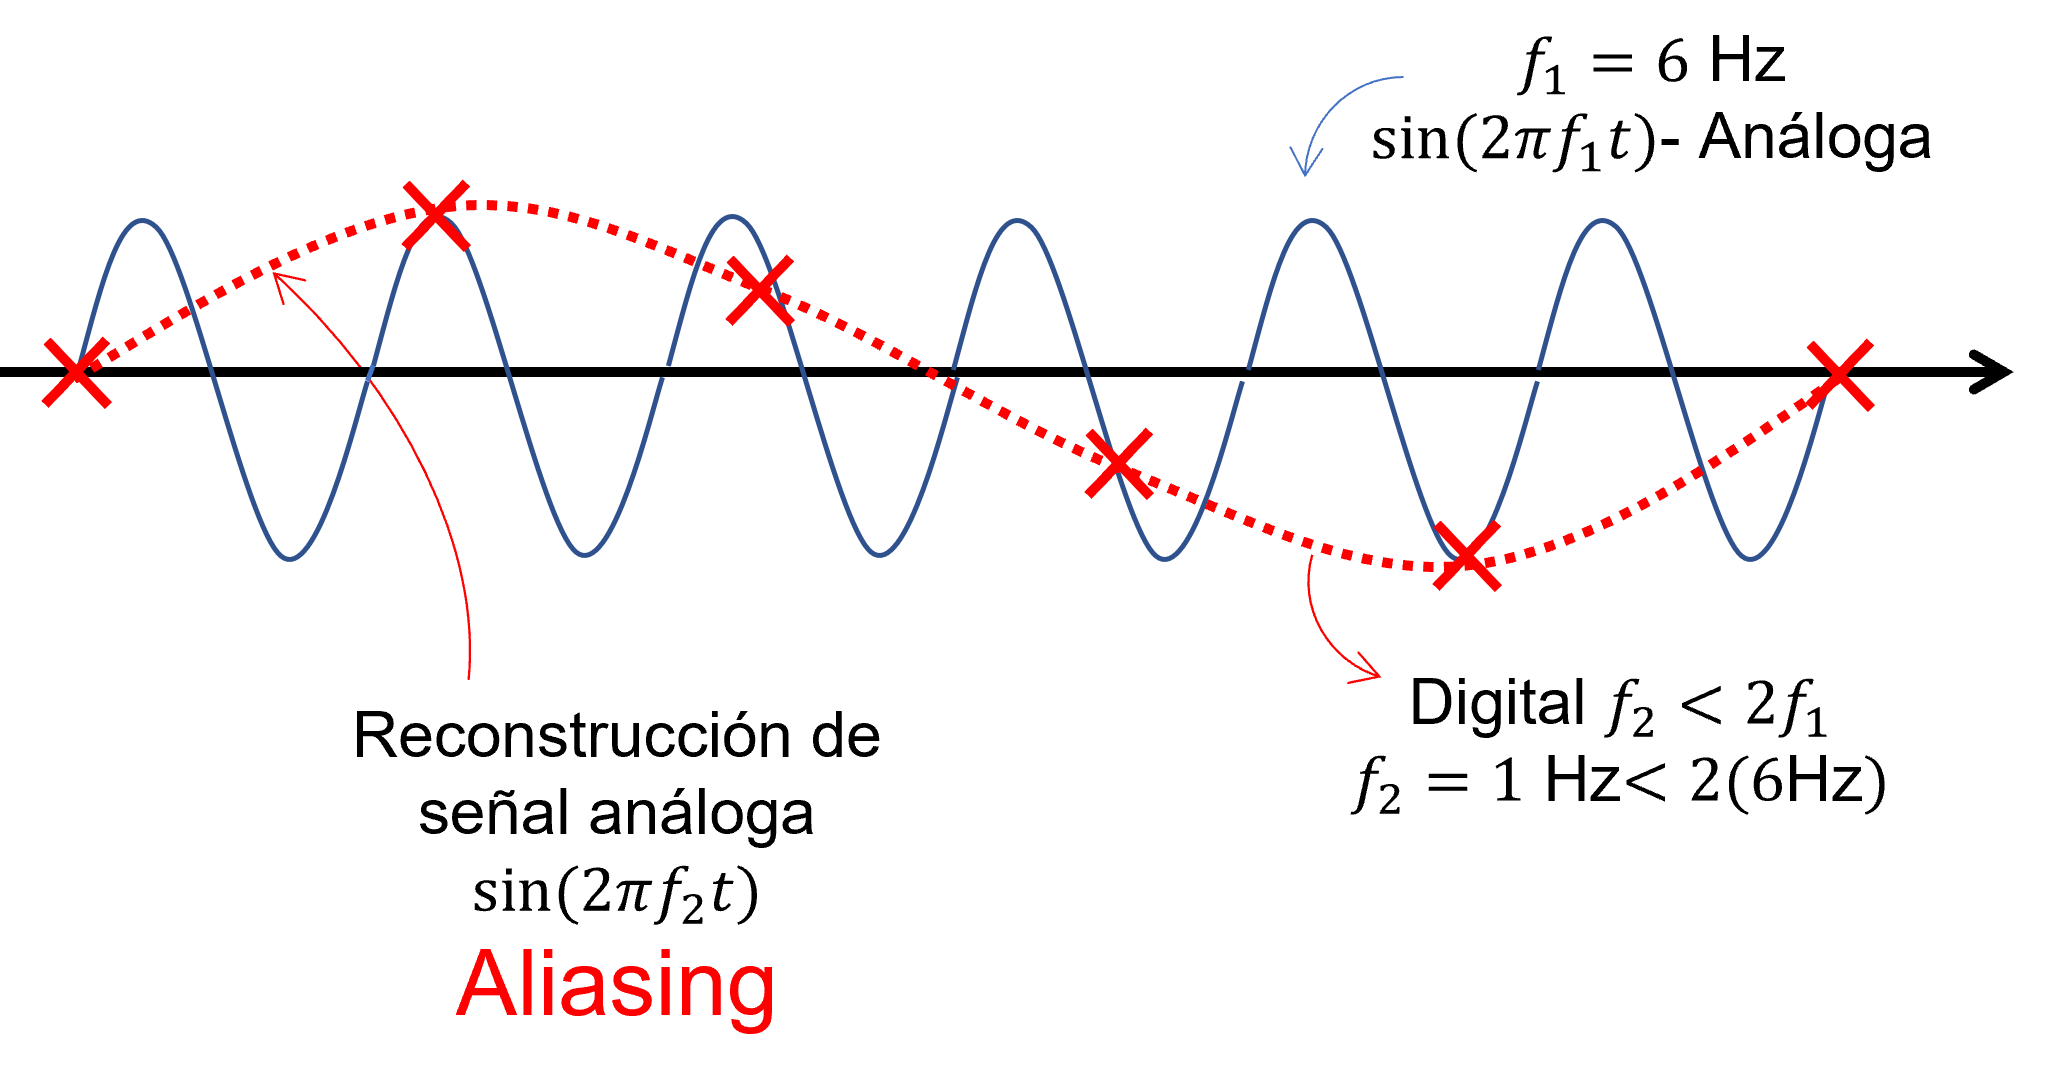
\includegraphics[scale=0.7]{Figuras/aliasing.png}
\end{figure}

\subsection{Aliasing en dominio de frecuencia}
Sin Aliasing:

\begin{figure}[H]
\centering
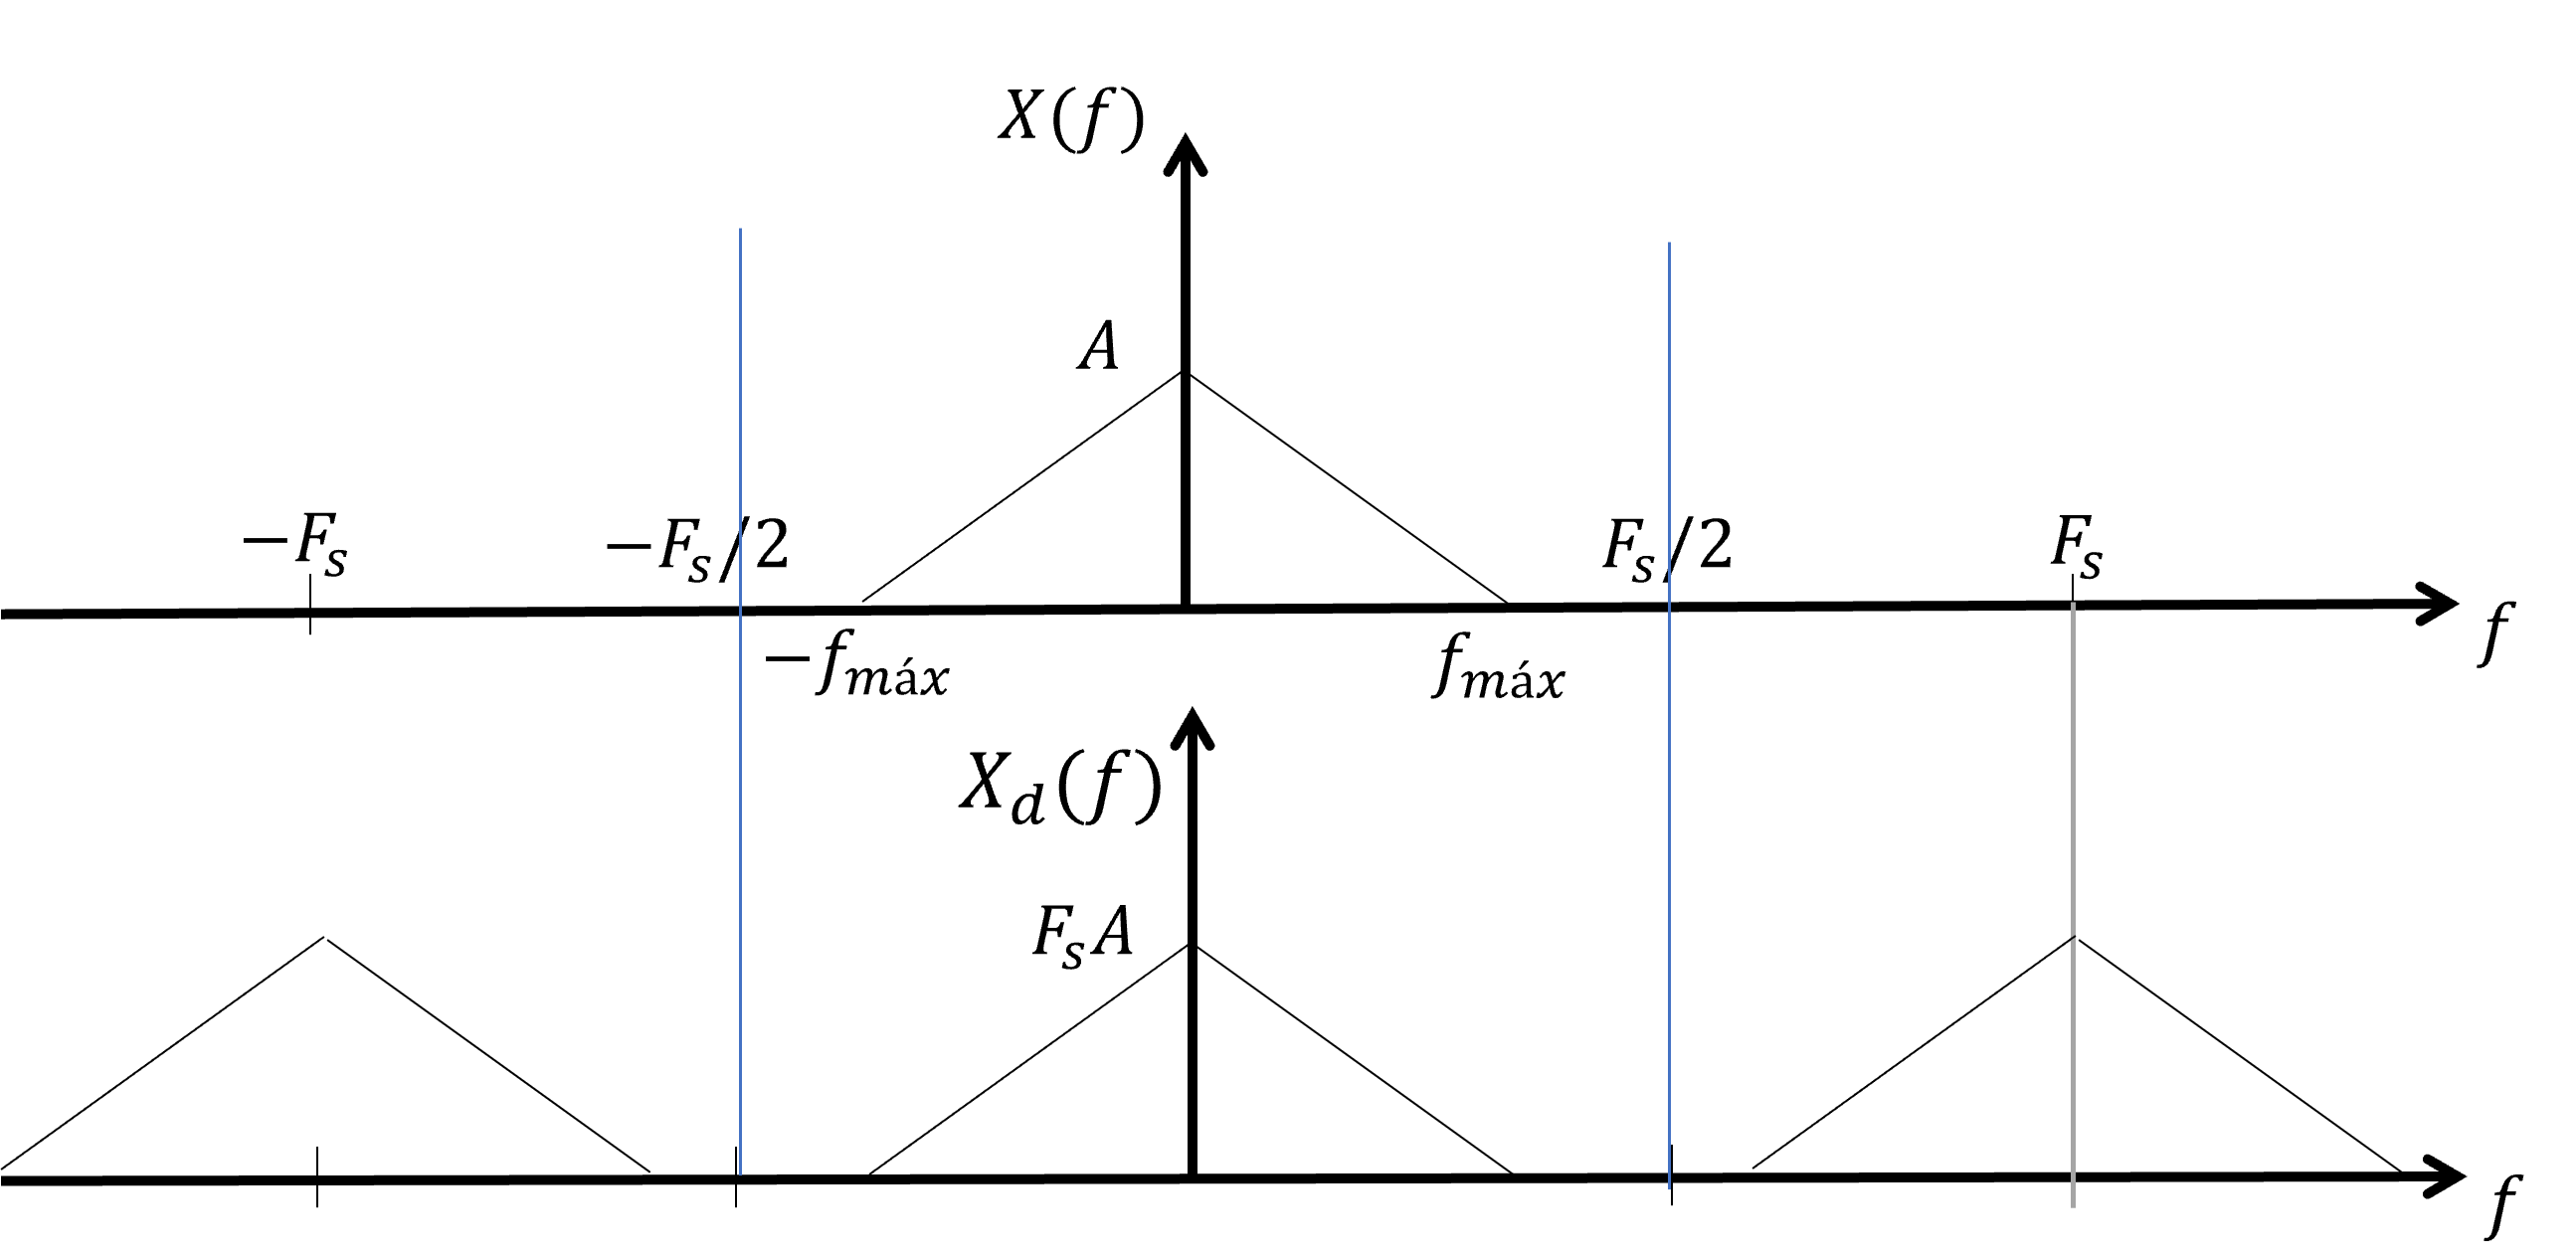
\includegraphics[scale=0.7]{Figuras/sin_aliasing.png}
\end{figure}

\begin{align*}
    Fs &> 2f_{max}\\
    f_{max} &< \frac{Fs}{2}=F_N \quad \text{frecuencia de Nyquist}
\end{align*}

\par Con Aliasing:

\begin{figure}[H]
\centering
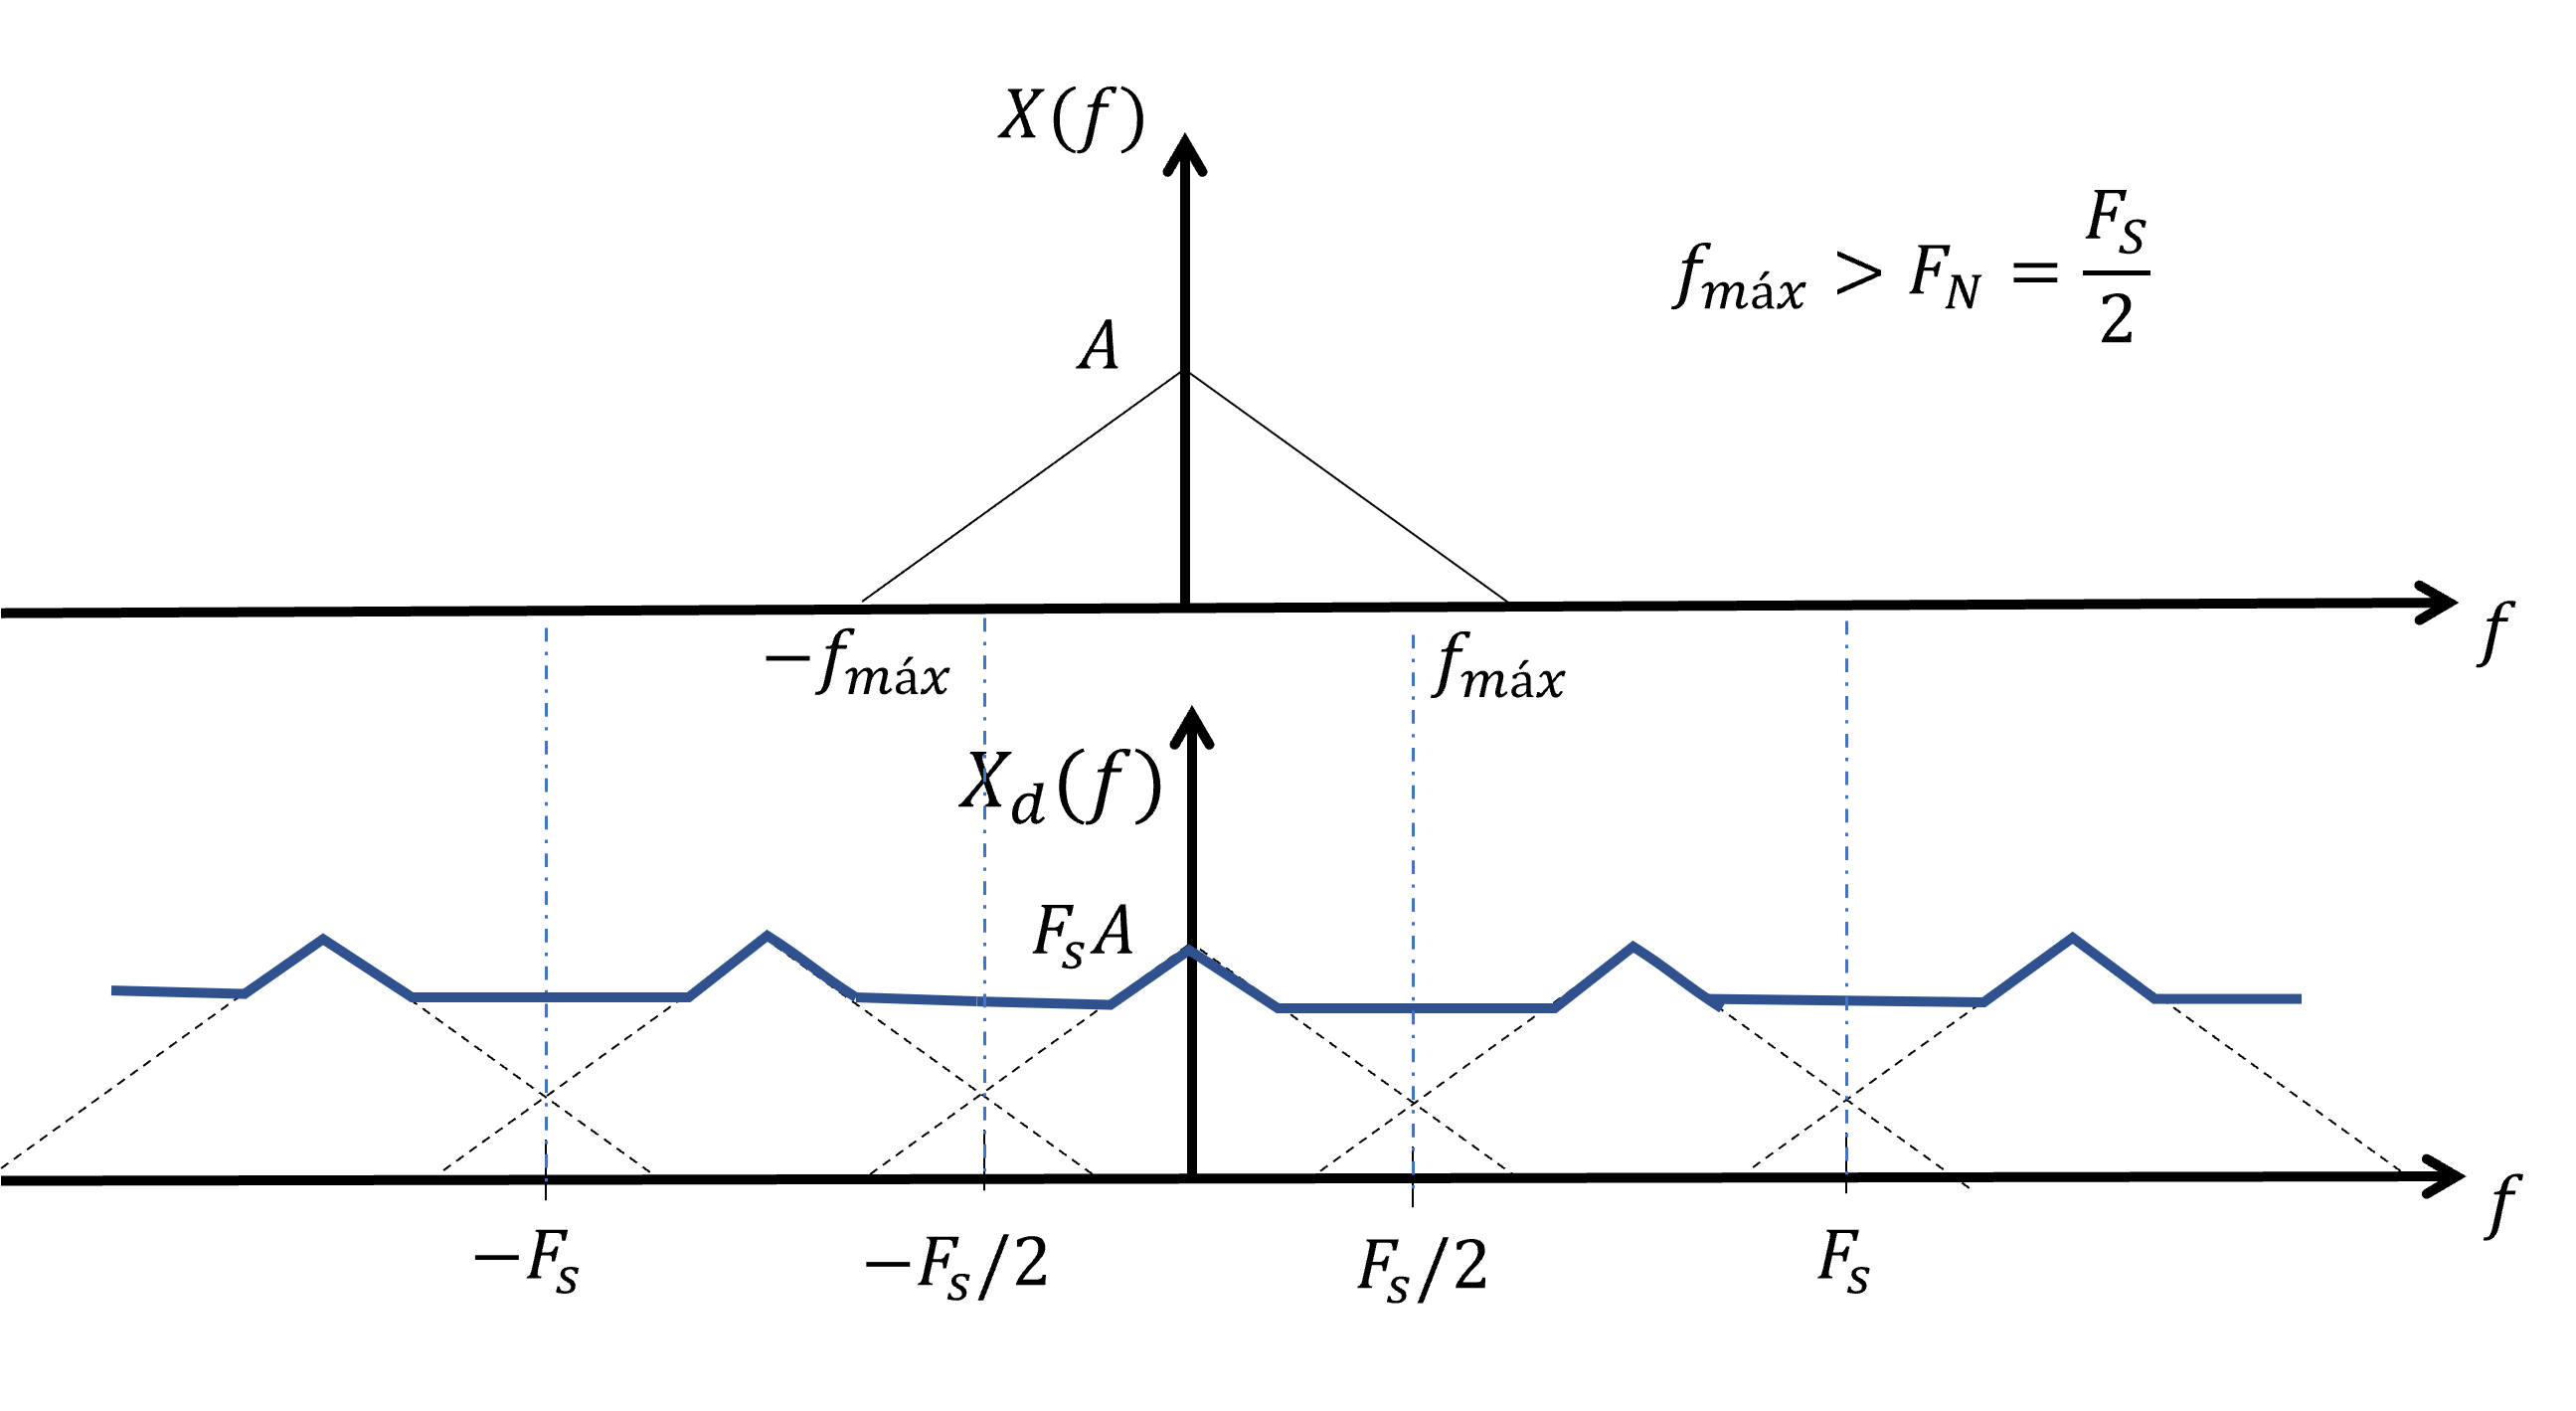
\includegraphics[scale=0.7]{Figuras/con_aliasing.png}
\end{figure}

\begin{figure}[H]
\centering
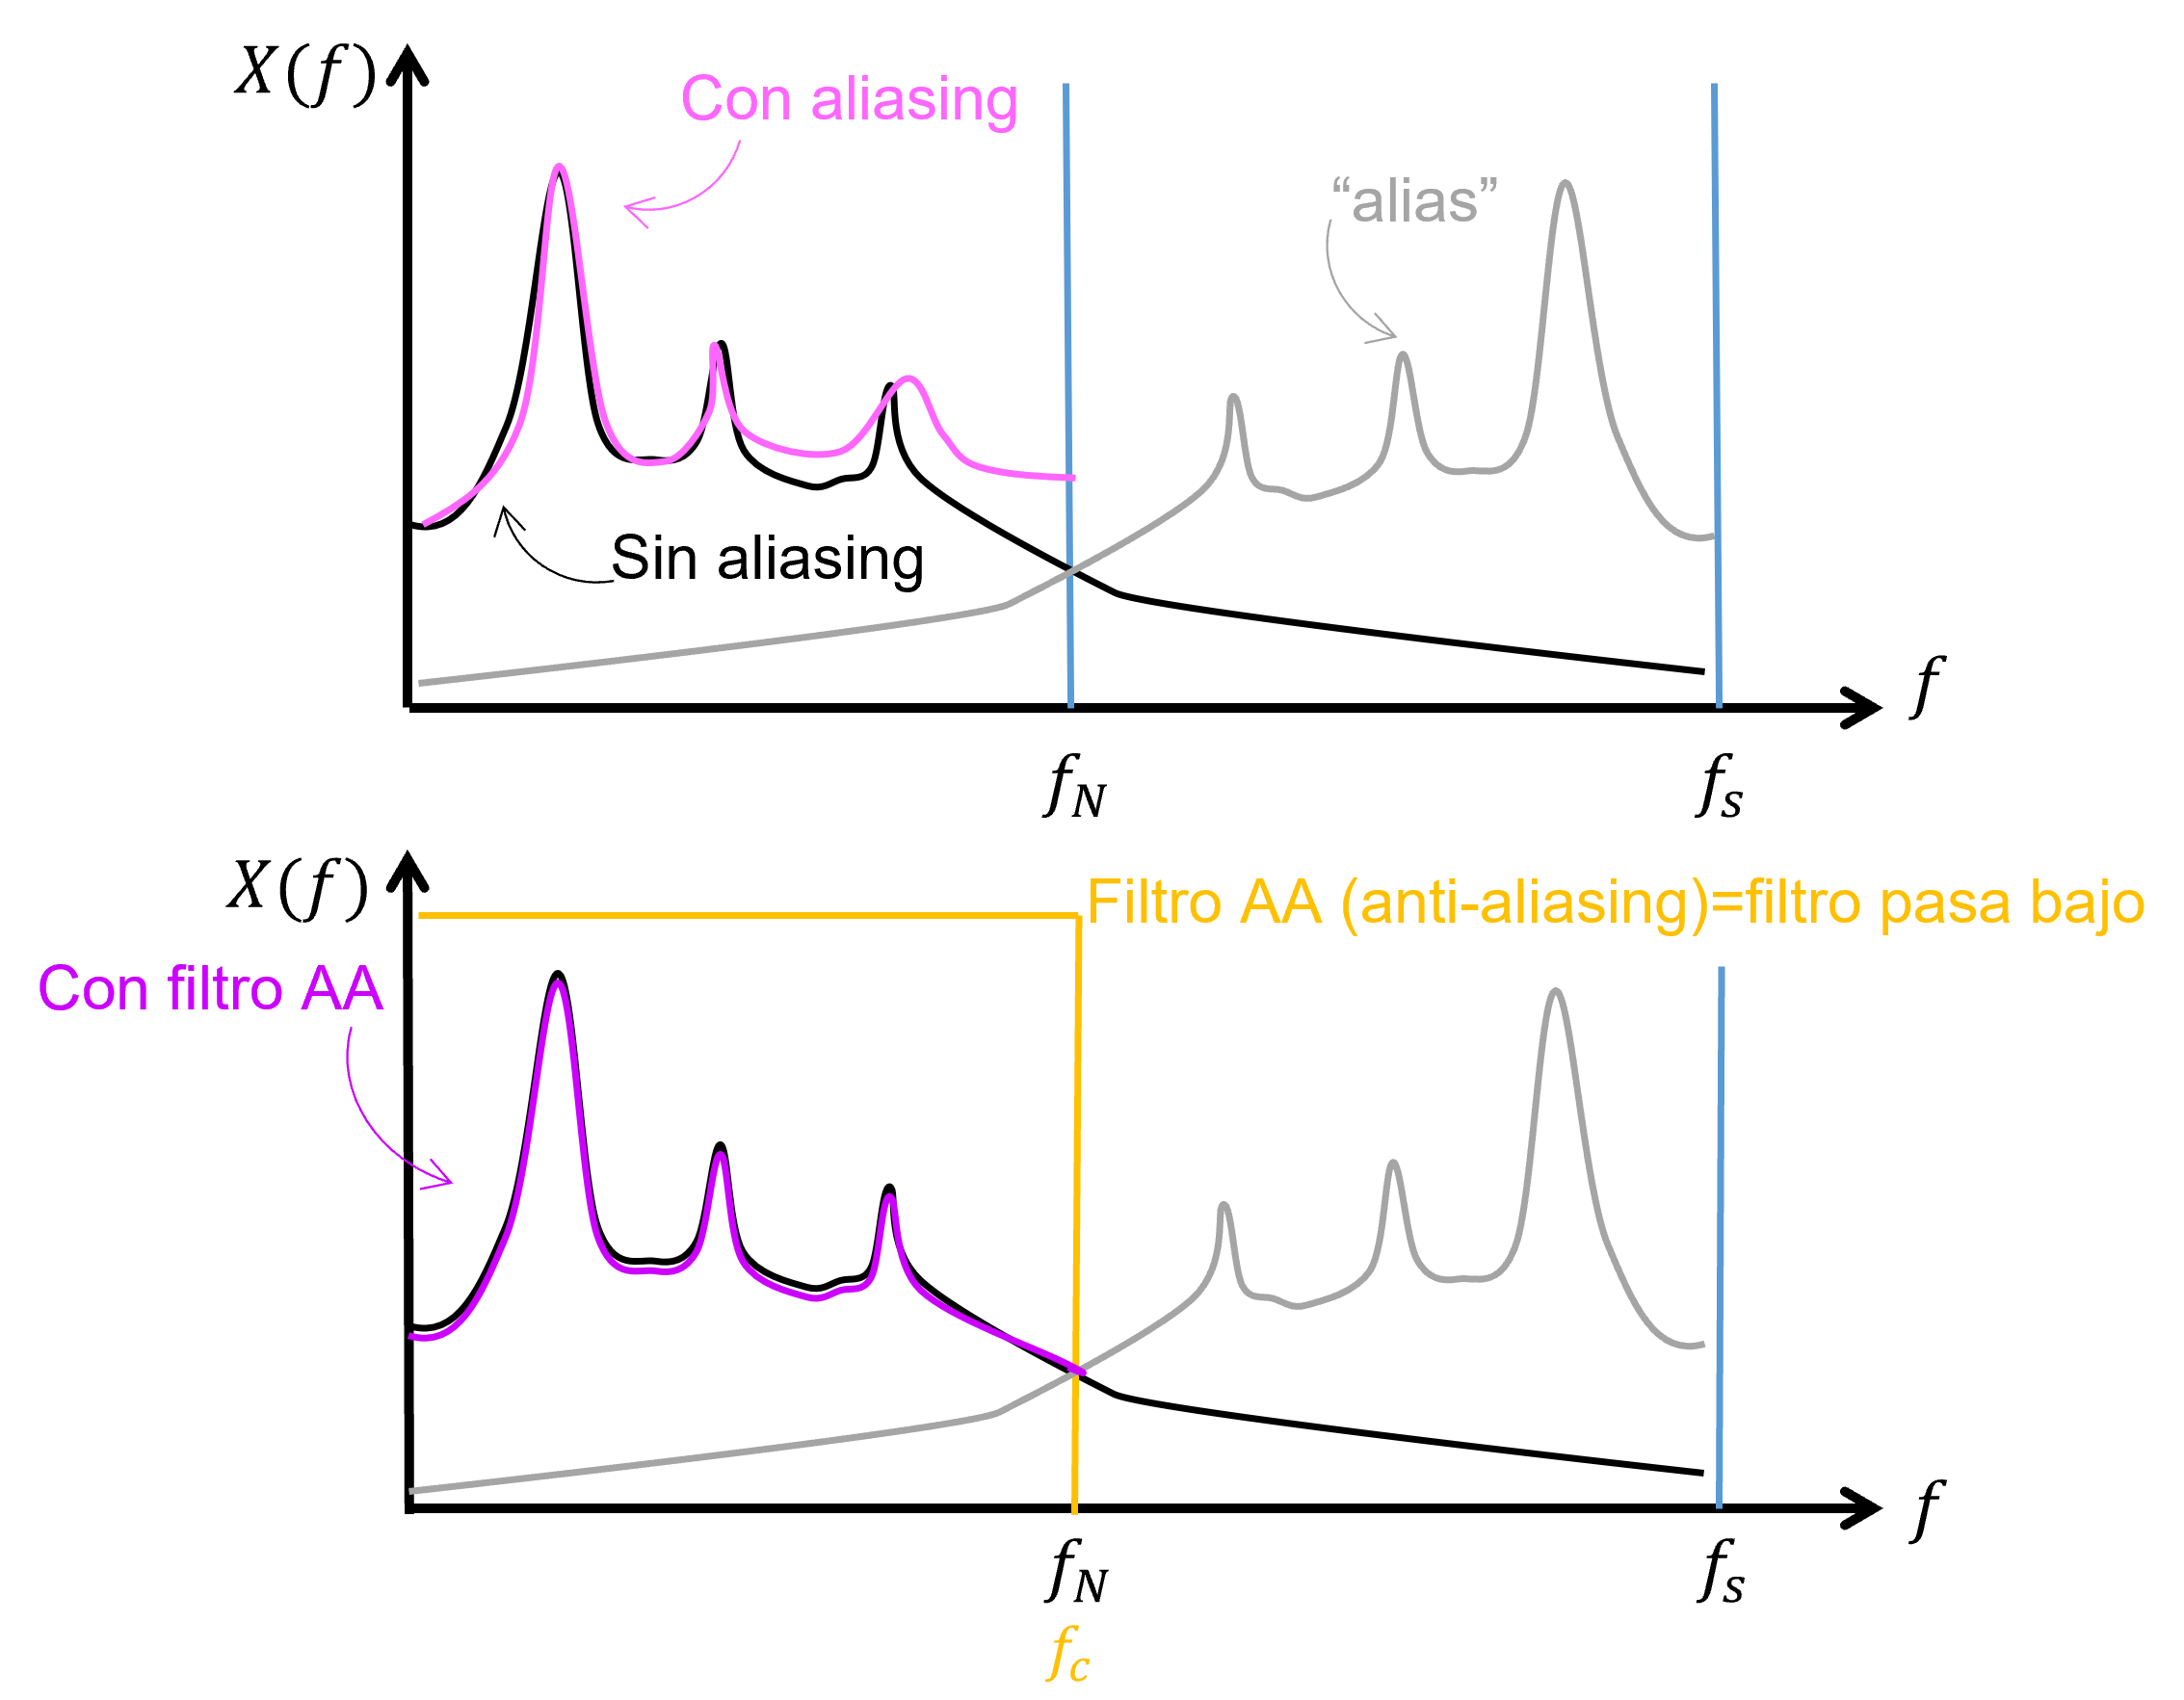
\includegraphics[scale=0.7]{Figuras/filtroAA.png}
\end{figure}

\begin{itemize}
    \item Filtro anti-aliasing es utilizado para eliminar el ``aliasing'' de la respuesta en frecuencia.
    \item Filtro AA tiene que ser aplicado antes del muestreo en el tiempo.
\end{itemize}

\begin{figure}[H]
\centering
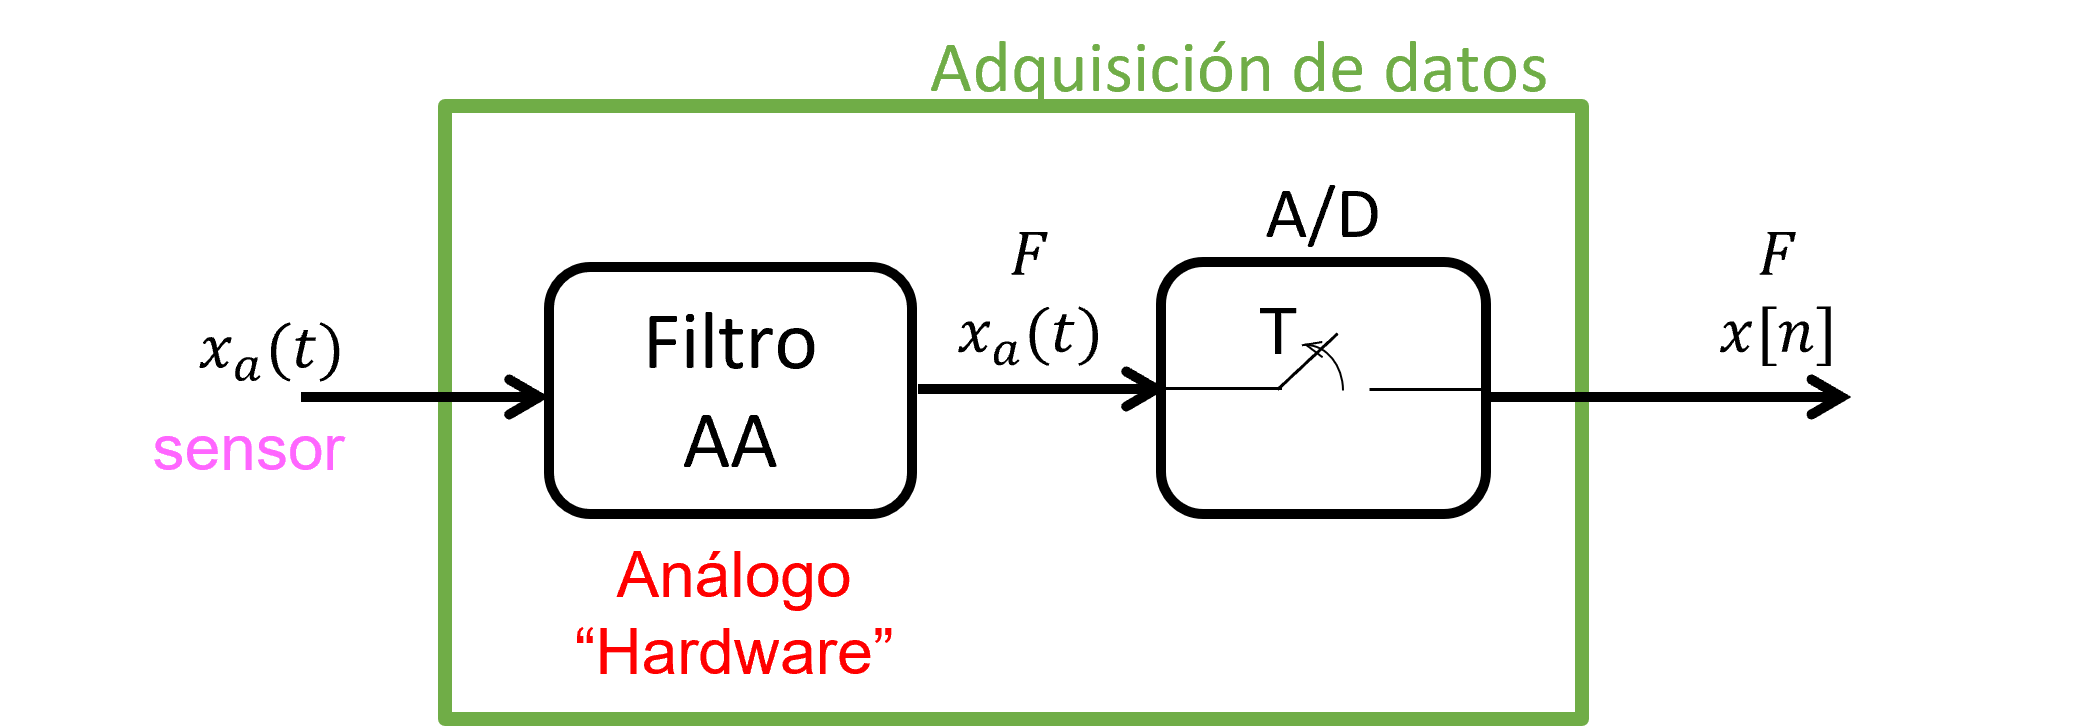
\includegraphics[scale=0.7]{Figuras/filtroAA2.png}
\end{figure}

\subsection{Spectral Leakage}
FT/DTFT/DFT asume que la señal es del tipo periódica.
$$ x(t) = x(t+T_1) $$
¿Qué pasa con señales no periódicas?
\begin{figure}[H]
\centering
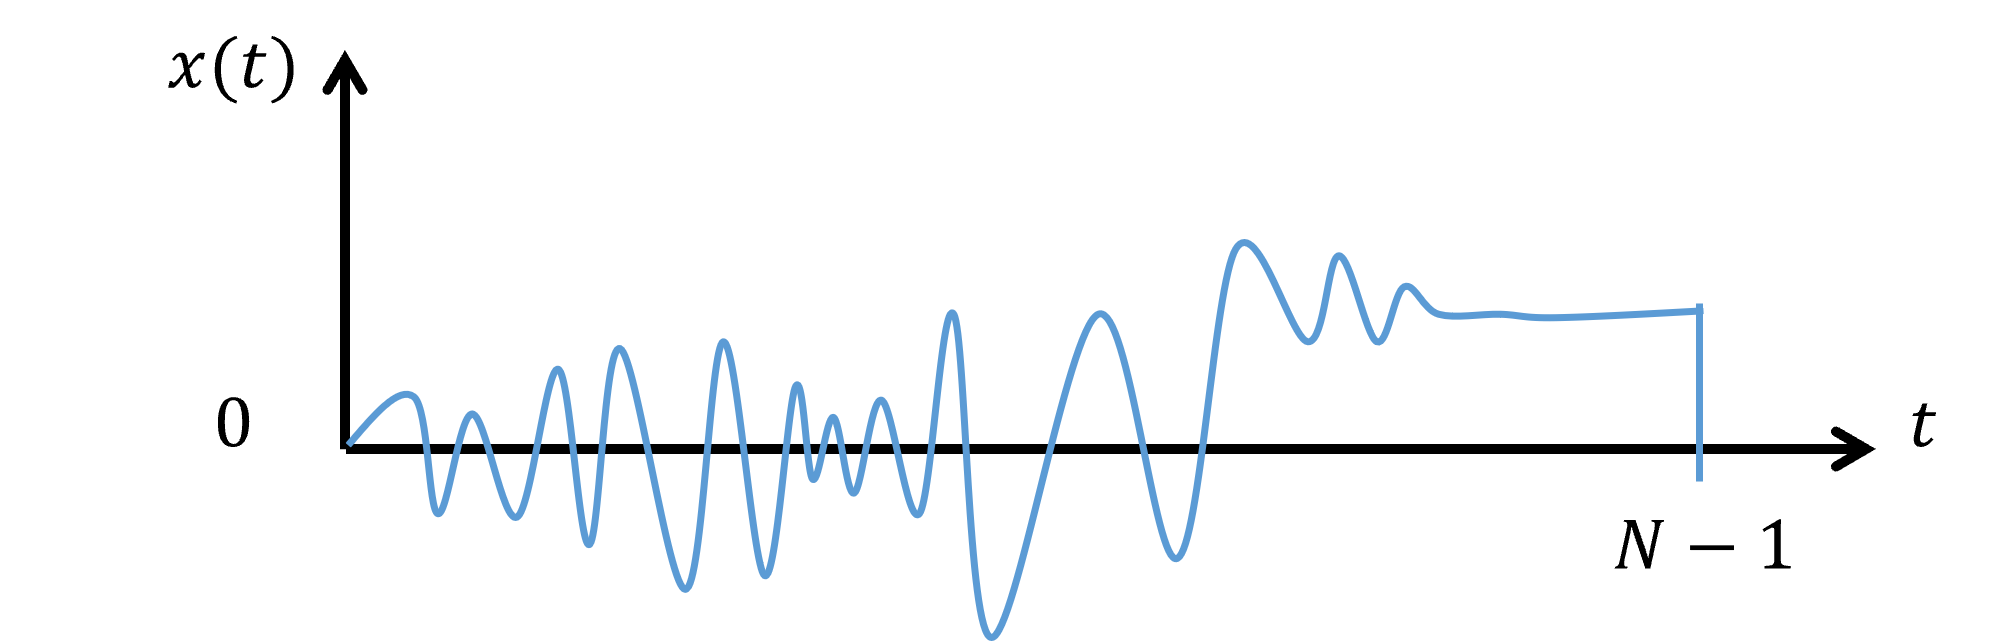
\includegraphics[scale=0.7]{Figuras/FT.png}
\end{figure}
DFT (N-pts): $X[m]=\sum_{n=0}^{N-1}x[n]e^{-j2\pi/N nm}$, $n$: 
indice tiempo, $m$: índice frecuencia
\begin{figure}[H]
\centering
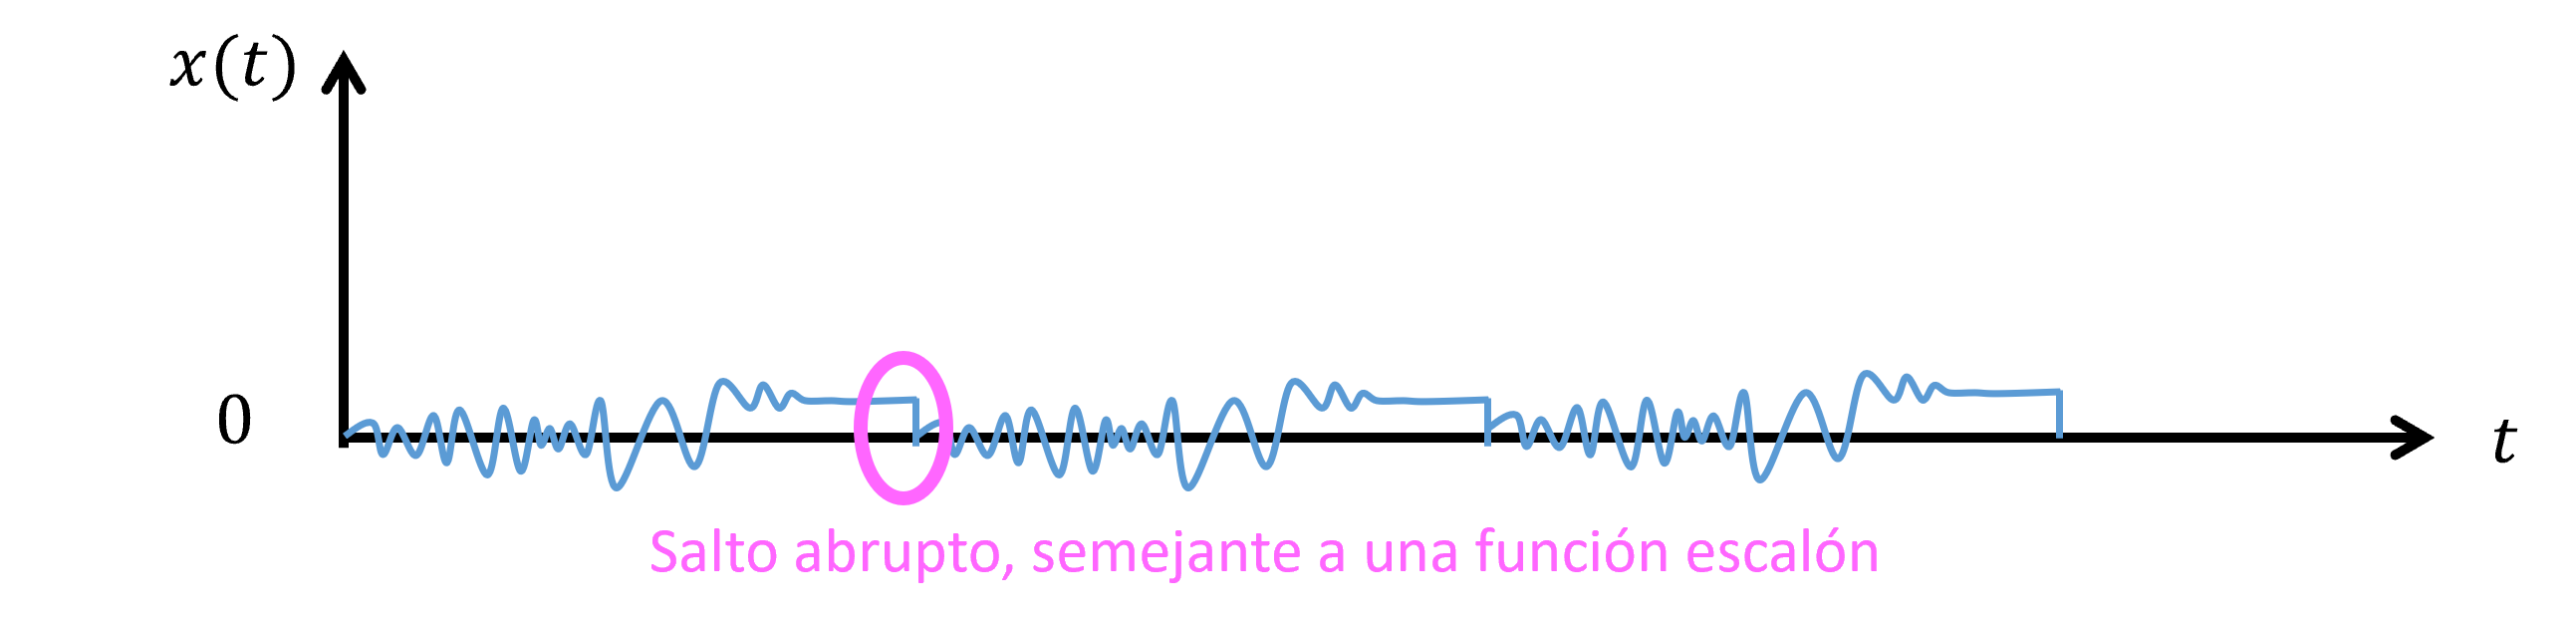
\includegraphics[scale=0.7]{Figuras/DFT.png}
\end{figure}

\par Una función escalón se puede escribir como una serie de Fourier (suma de armónicas).\\

\par Al calcular $X[m]$ (DFT de $x[n]$) surge el fenómeno de ``spectral leakage'', donde se agregan armónicas artificiales producto del escalón generado.\\
\par \underline{Ejemplo}:

\begin{figure}[H]
\centering
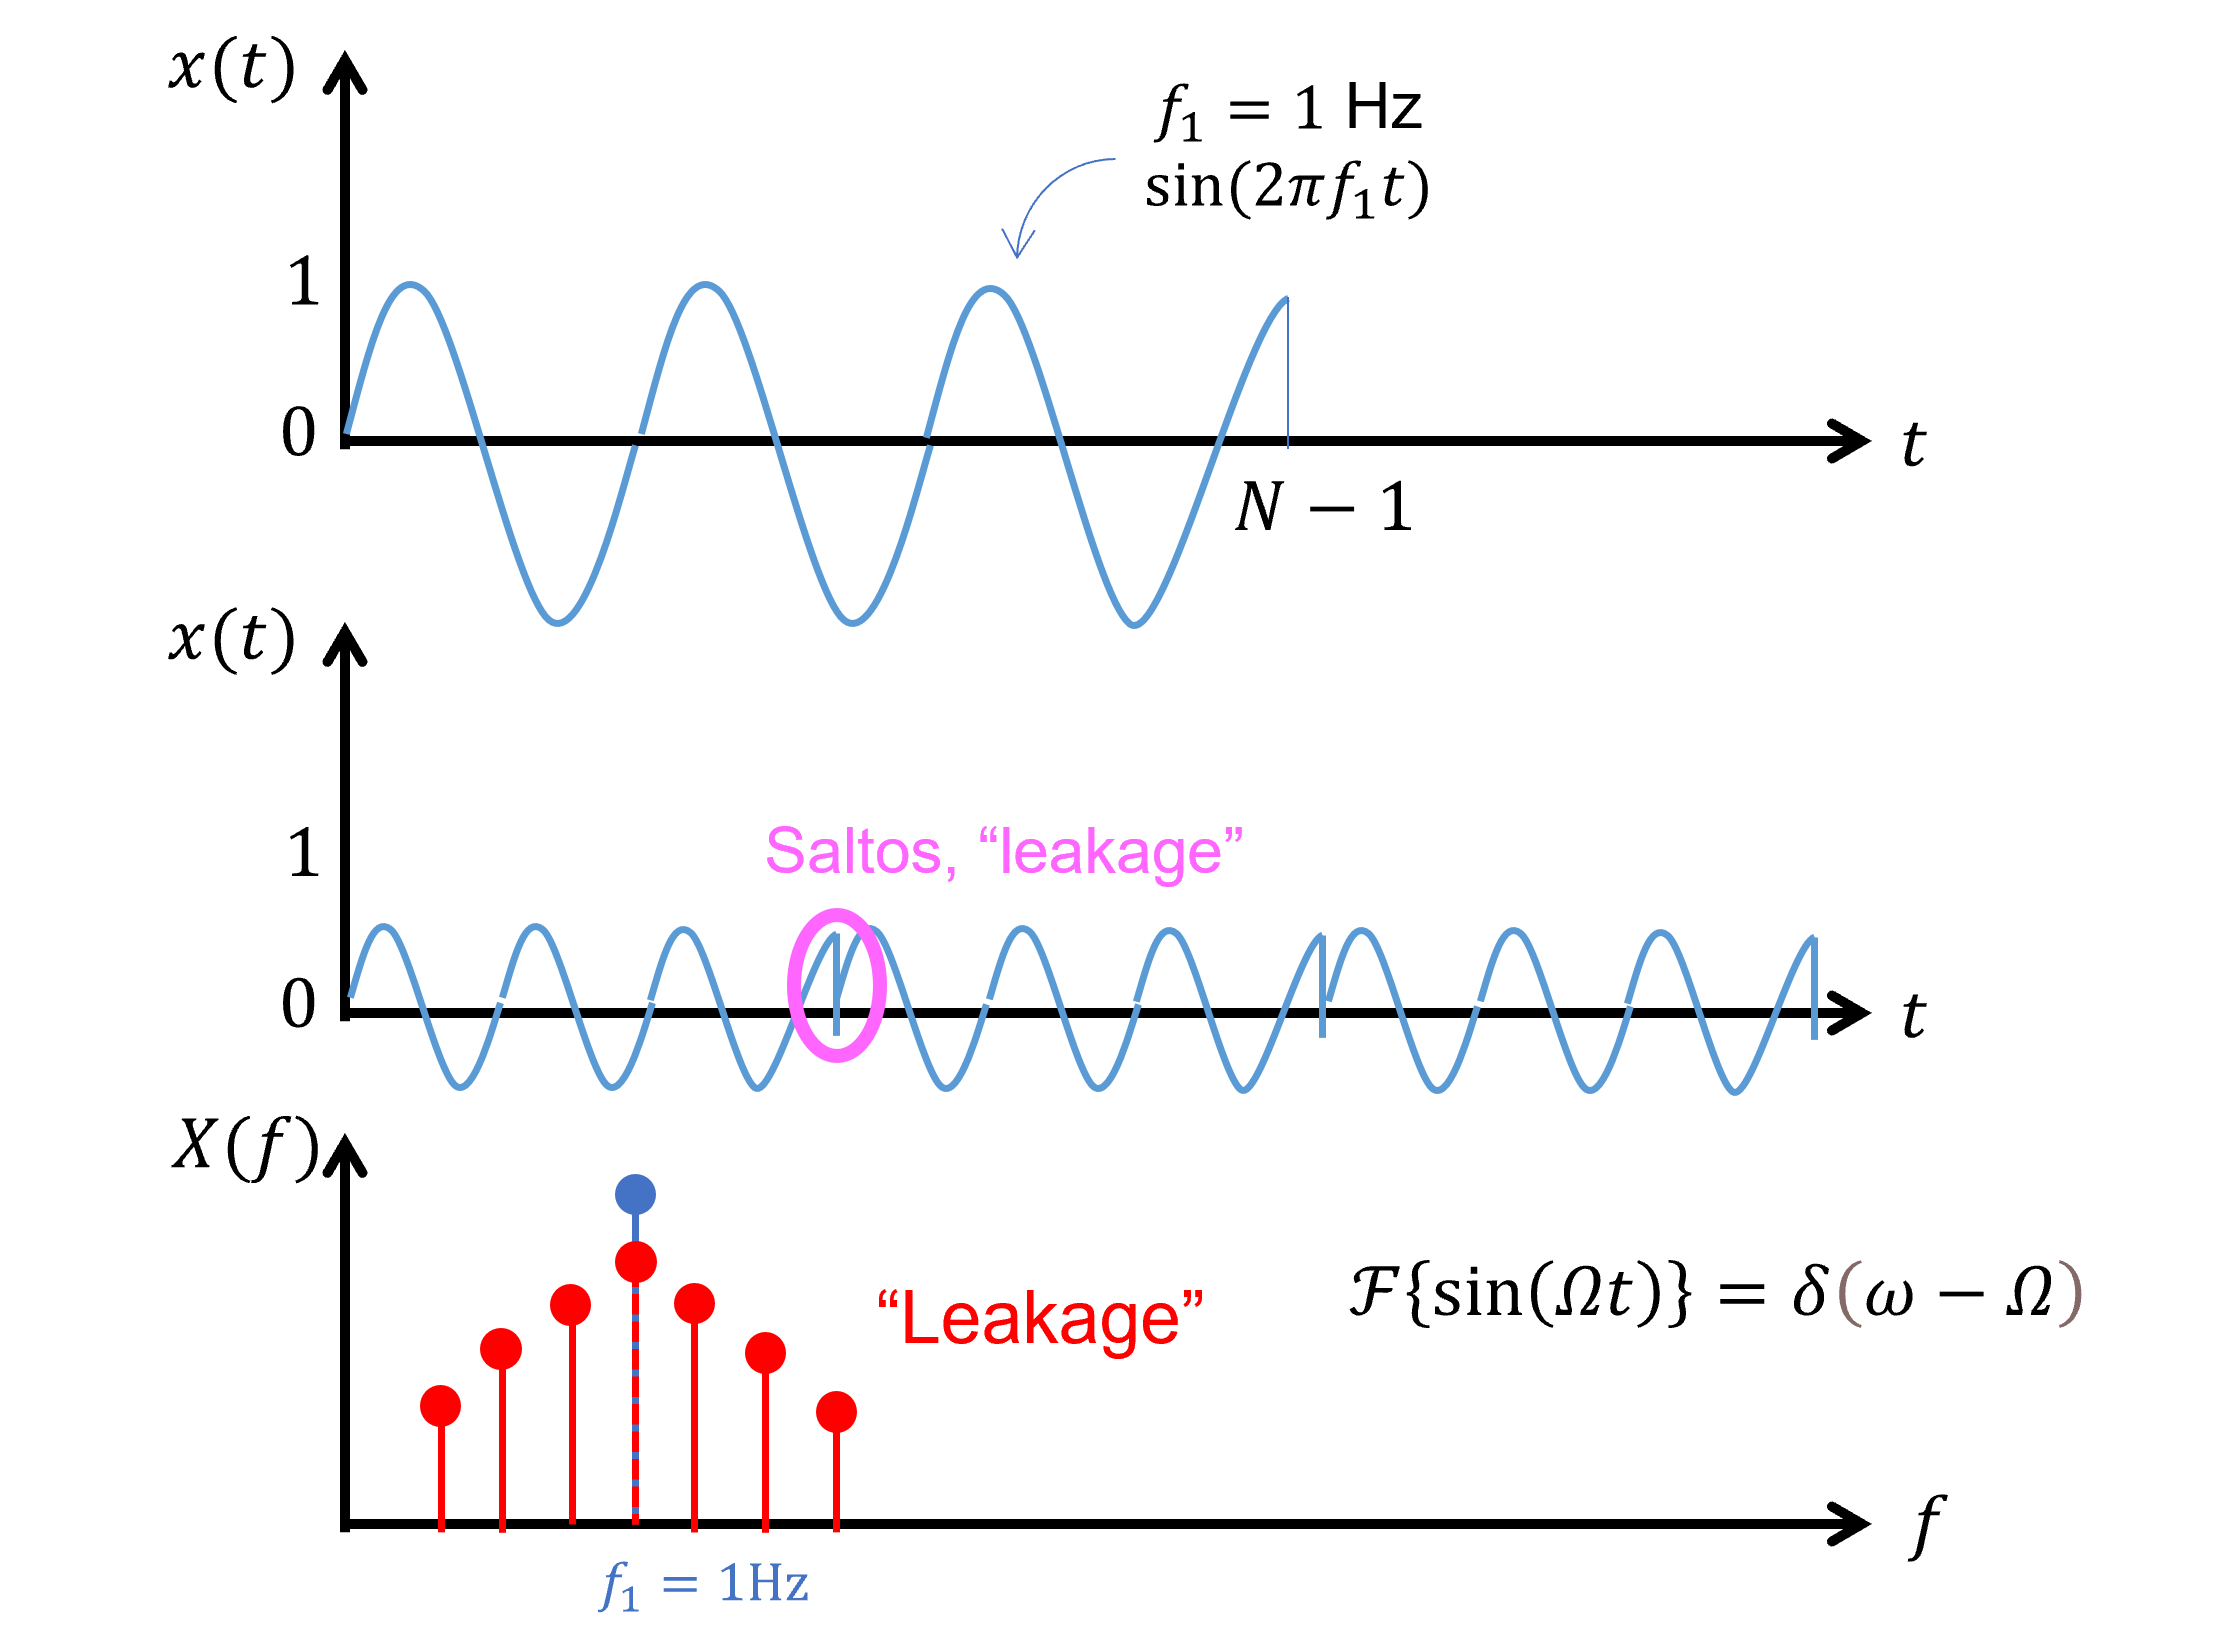
\includegraphics[scale=0.7]{Figuras/ejemplo_leakage.png}
\end{figure}

\par \underline{Solución}: ``Windowing'' $\Longrightarrow$ aplicar ventanas.\\
\par Sobre el cálculo de PSD en registros digitales: 

\begin{figure}[H]
\centering
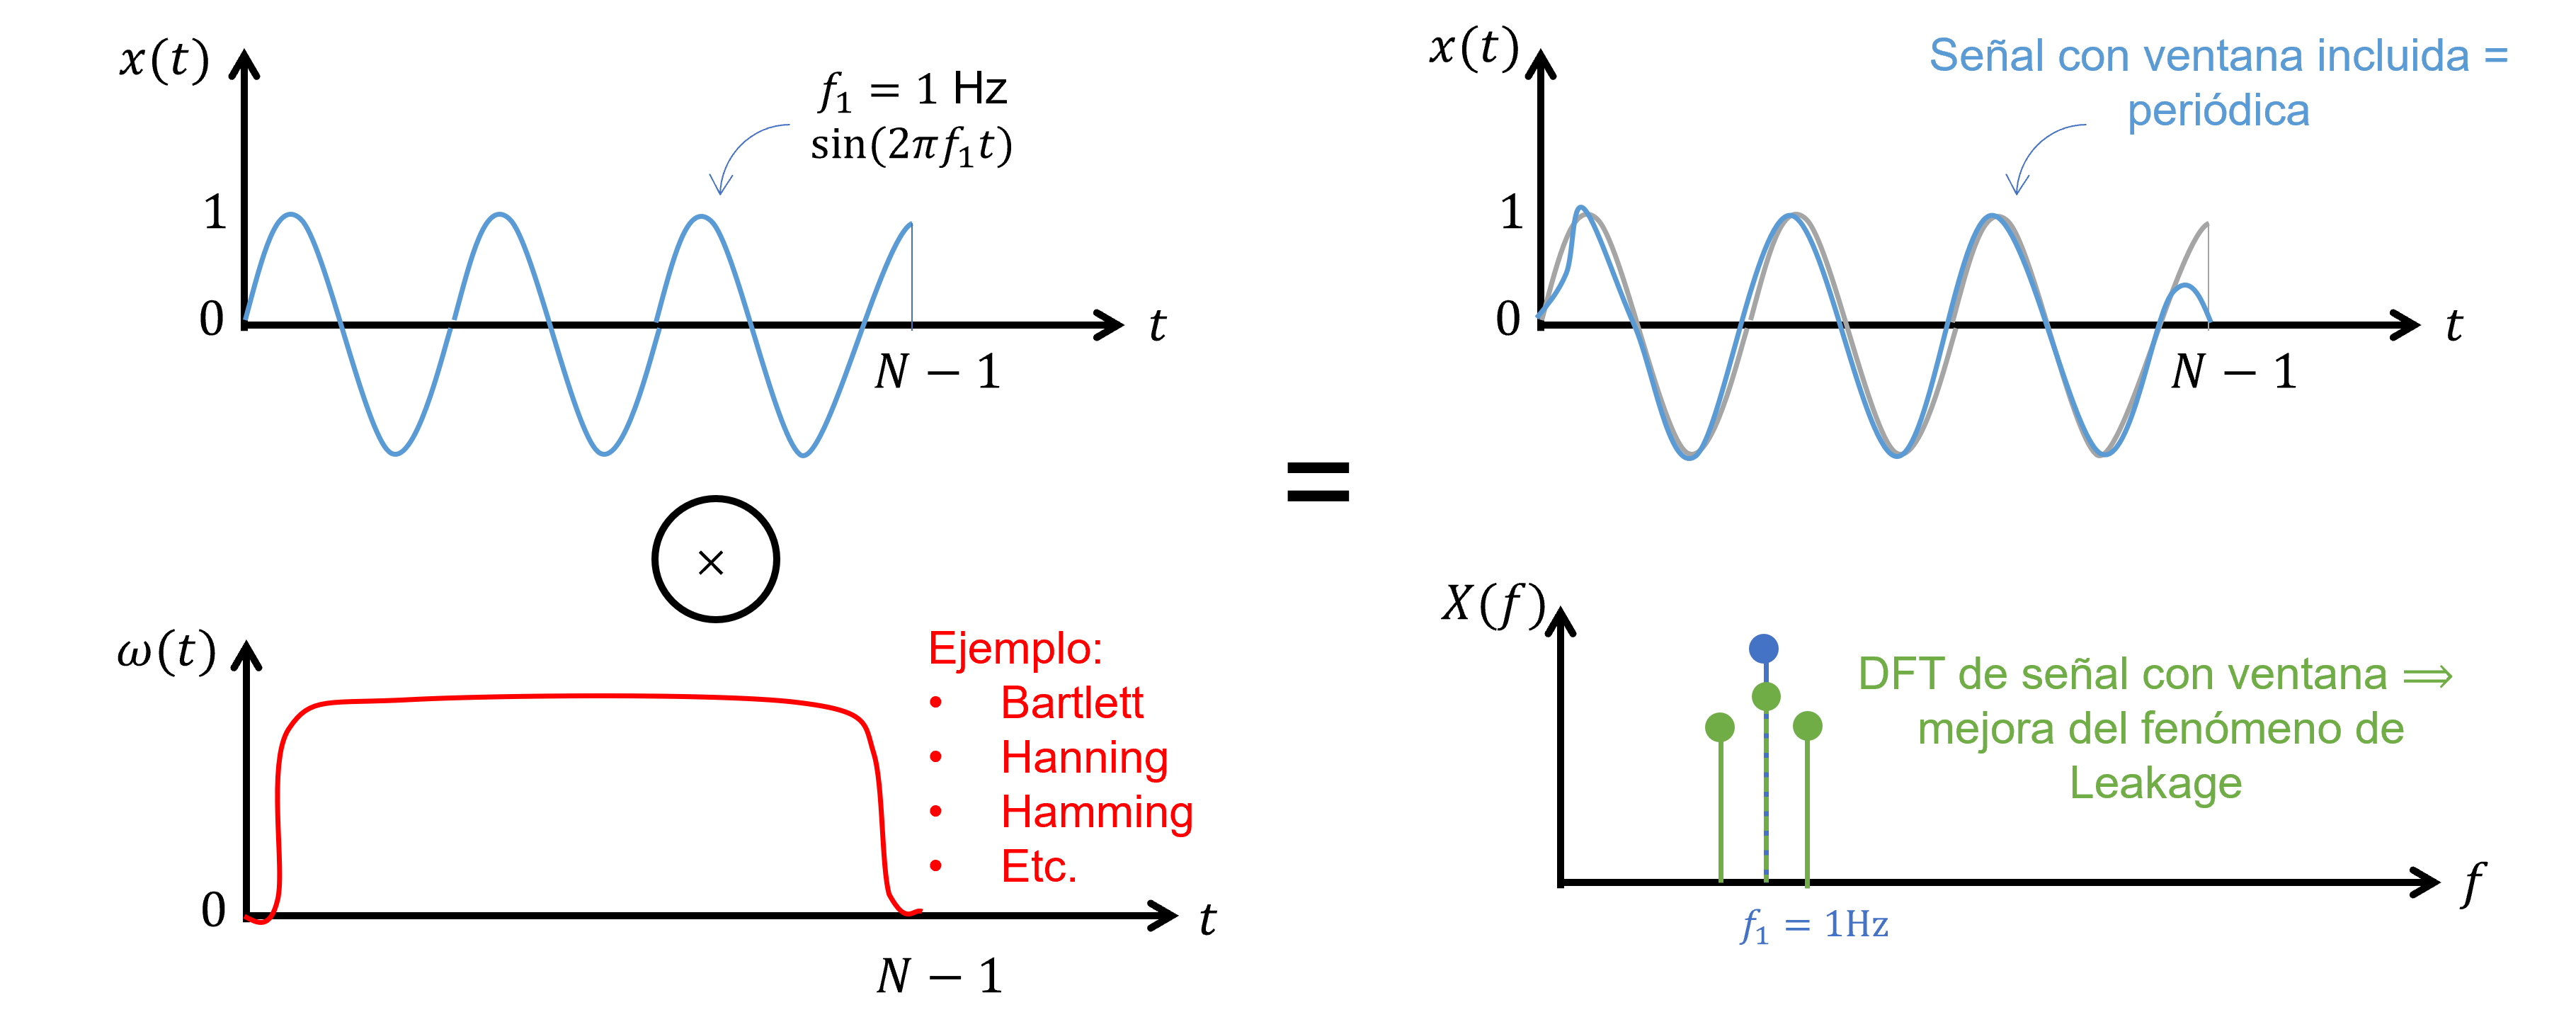
\includegraphics[scale=0.6]{Figuras/solucion_leakage.png}
\end{figure}

\begin{align*}
    u(t)\xrightarrow[]{\text{Auto-PSD}} S_{UU}(\omega)=\mathcal{F}\{R_{UU}(\tau)\}\\
    \Longrightarrow S_{UU}(\omega) = \mathcal{F}\Bigl\{\mathbb{E}\{u(t)u(t+\tau)\}\Bigr\}
\end{align*}

Cómo calcular $S_{UU}(\omega)$ con una señal digital? $\Longrightarrow$ Periodograma.


\section{Motivación}
Sea $x[k]$ un proceso estocástico wss (estacionario sentido amplio), señal digital con un intervalo de muestreo T.
\begin{align*}
    S_X(\omega) &= \mathbb{F}\{R_x(\tau)\} \quad \text{(Caso contínuo)}\\
    &= \mathbb{E}\{X(\omega)X^\ast(\omega)\} \quad \text{(Caso contínuo)}
\end{align*}

Podemos estimar $S_x(\omega)$ utilizando estimadores de valor medio y la definición de DTFT.

\begin{align*}
    S_x(\omega) \sum_{k=-\infty}^{+\infty}\hat{r}_x[k]e^{-j\omega k}
\end{align*}
donde $\hat{r}_x[k]=\frac{1}{N}\sum_{n=1}^Nx[n]x[n+k]$ estimador de autocorrelación.\\

\par Alcance para la estimación del PSD:
\begin{enumerate}
    \item Calcular DFT, y utilizar una forma de calcular el promedio de manera insesgada.
    \begin{figure}[H]
    \centering
    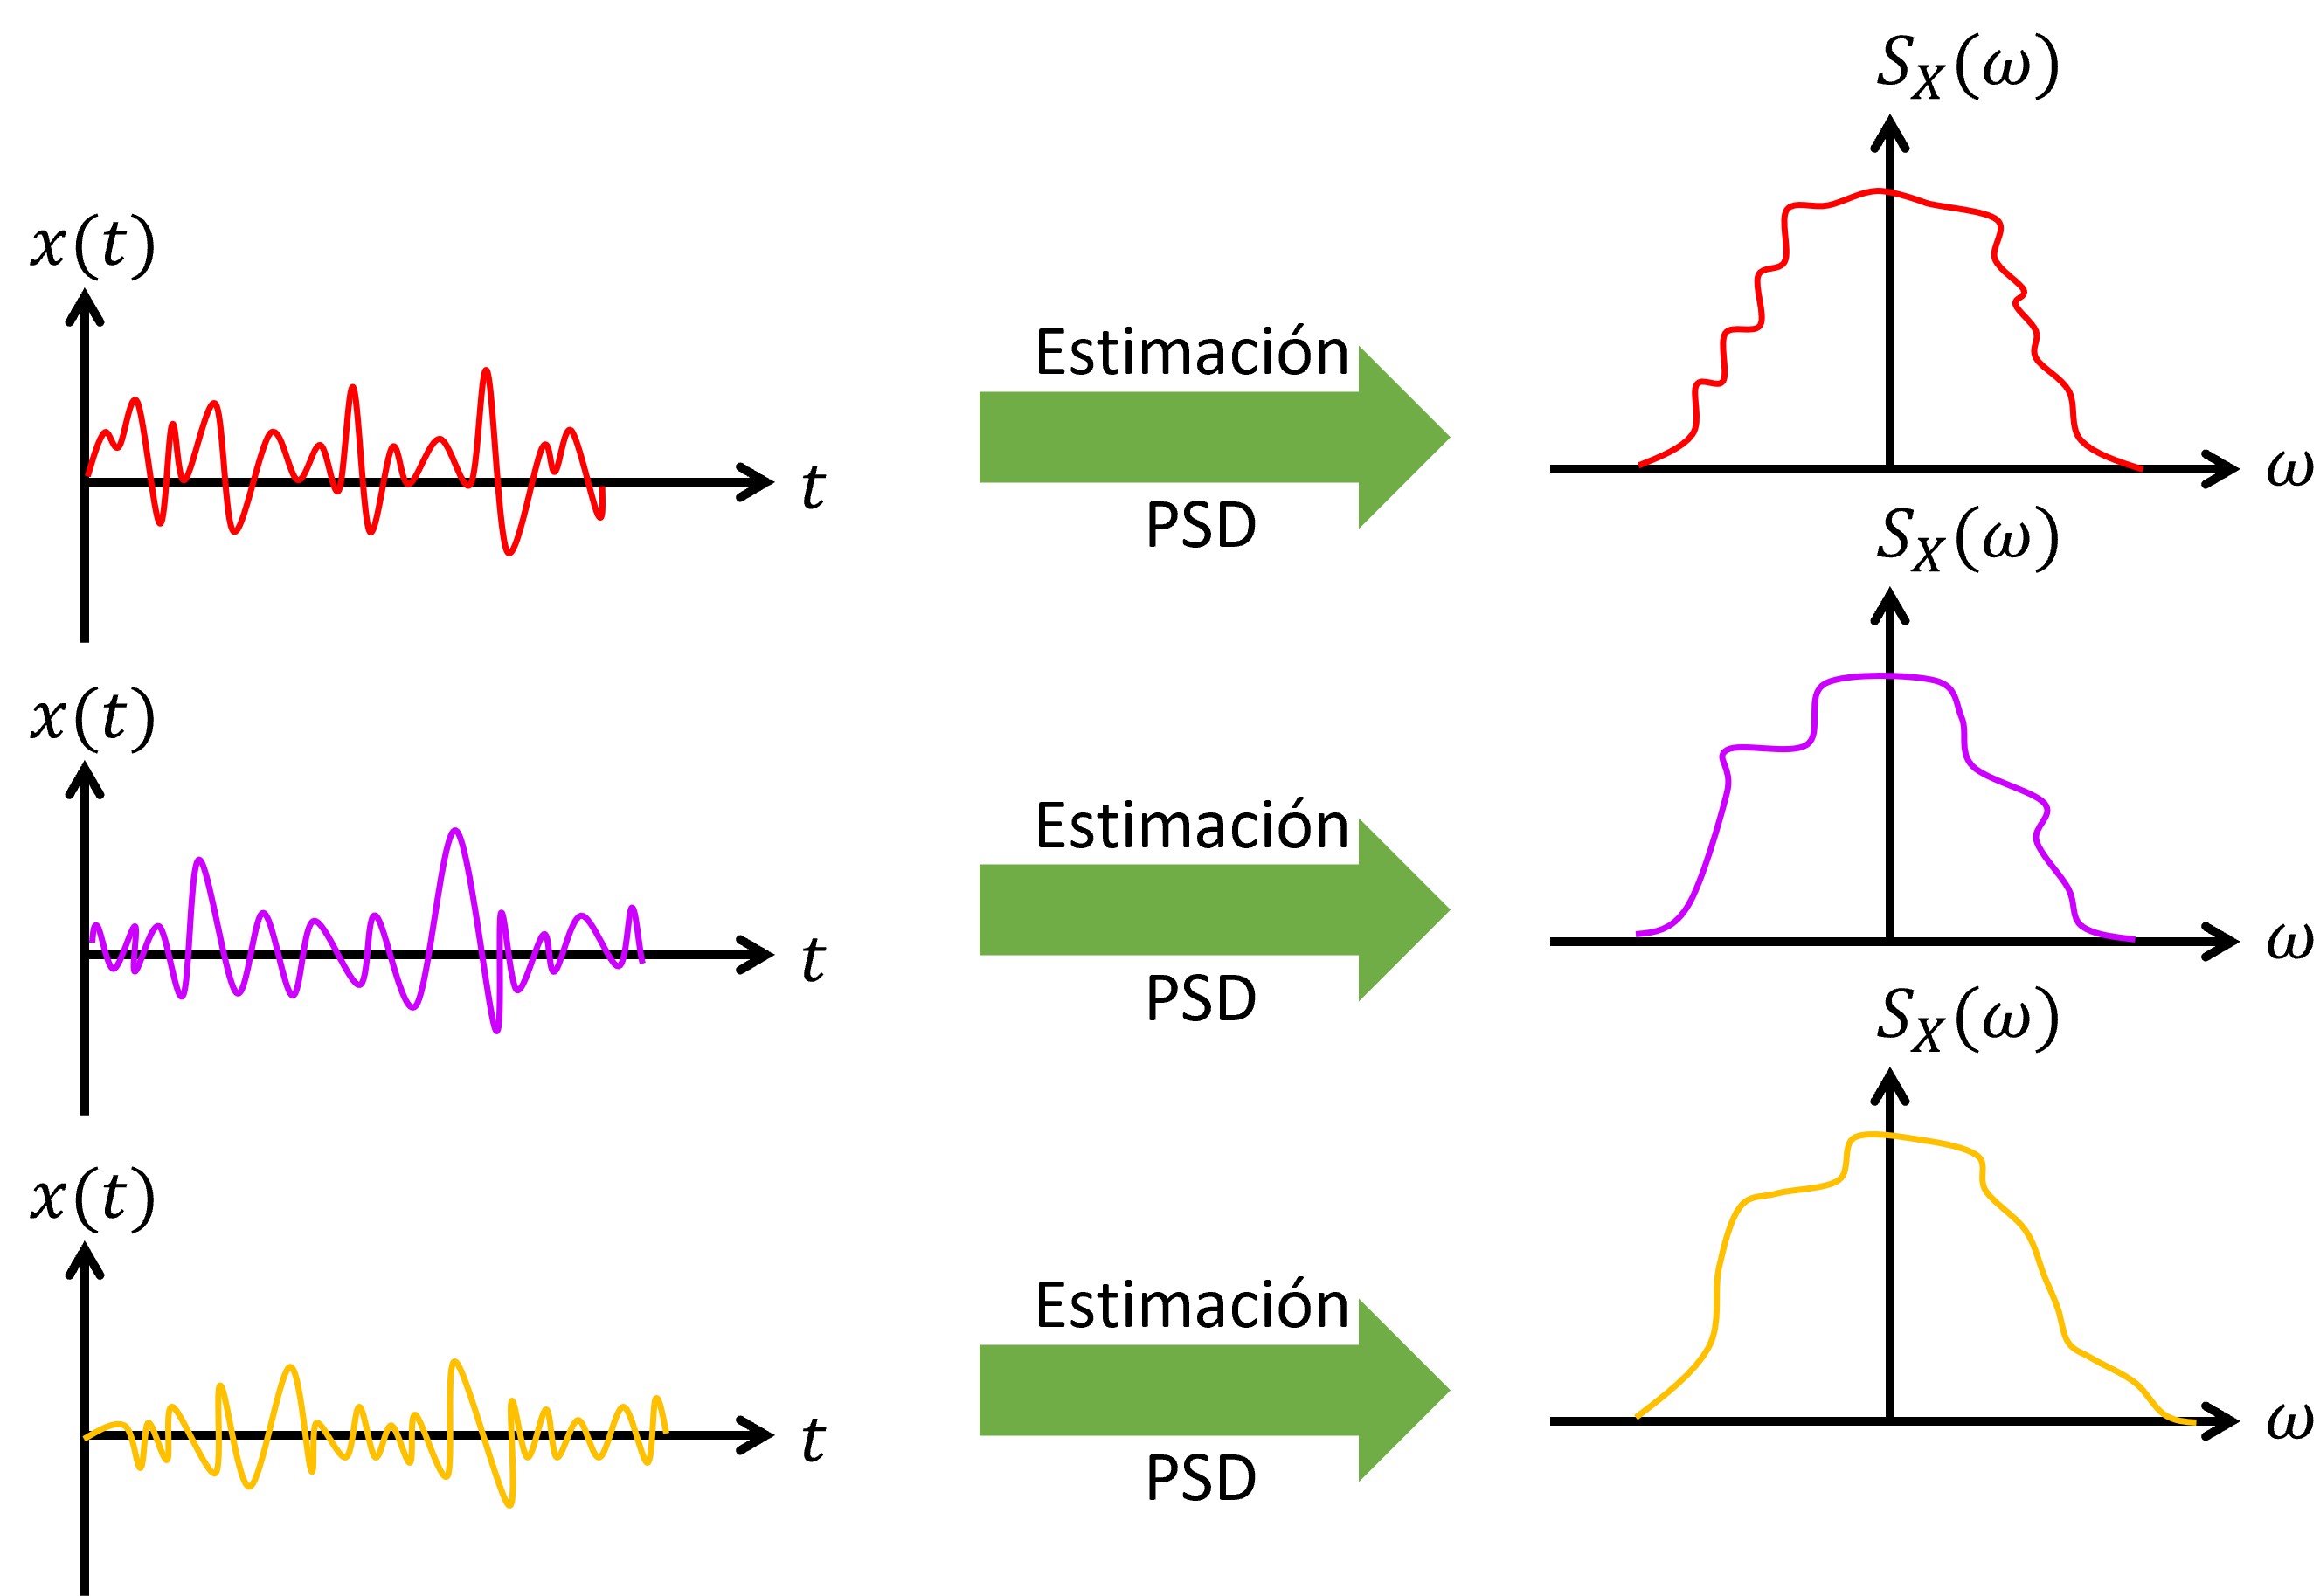
\includegraphics[scale=0.6]{Figuras/PSD_realizaciones.png}
    \end{figure}
    \item Tres realizaciones de $x[k]$ nos entegan disintas estimaciones del PSD.
\end{enumerate}

Cada estimación del PSD es una realización de un proceso estocástico.\\
\par Vamos a caracterizar el PSD utilizando la media y varianza:
\begin{enumerate}
    \item Queremos que la media del PSD se acerque al valor real del PSD.
    \item Queremos que la varianza del PSD sea pequeña.
\end{enumerate}

\underline{Ejemplo}: Considere el sgte. p.e.:
\begin{align*}
    x[n]=A+\omega[n]
\end{align*}
donde $A$ es una constante y $\omega[n]$ es ruido blanco, de media cero, $\sigma^2$.\\
\par Dada una secuencia finita $\{x[0],x[1]...,x[N-1]\}$, estimar A:\\
\par Estimador razonable: $\hat{A}=\frac{1}{N}\sum_{n=0}^{N-1}x[n]$ ``media muestral de A''.\\
\par Queremos dos cosas:
\begin{enumerate}
    \item Que $\hat{A}$ converja al valor correcto de $A$: 
    $$\mathbb{E}\{\hat{A}\}=A \quad \text{ estimador es insesgado}$$
    Sino, $\hat{A}$ es sesgado. Si no se cumple, pero $$lim_{N\to\infty} \mathbb{E}\{\hat{A}\}=A \quad \text{estimador asintóticamente insesgado} $$
    \item La varianza de $\hat{A}$ sea pequeña
    $$\text{var}\{\hat{A}\}\to 0 \quad \text{quizás aumentando N se disminuye la dispersión de }\hat{A}$$
\end{enumerate}

\underline{Objetivos}: Estimar $\hat{S}_x(\omega)$ tal que:
$$\mathbb{E}\{\hat{S}_x(\omega)=S_x(\omega) $$ y 
$$\text{var}\{\hat{S}_x(\omega)\}=\text{pequeño} $$ 

\section{Periodograma}
\underline{Definición}: 
\begin{align*}
    \hat{S}_{PER}[k] =\frac{1}{N}\bigg|\sum_{n=0}^{N-1}x[n]e^{-j2\pi nk/N}\bigg|^2
\end{align*}

\underline{Nota}: 
\begin{enumerate}
    \item Considera el cálculo del DFT en vez de TF contínua
    \item Considera un estimador neutral para el cálculo de la $\mathbb{E}\{\cdot \}$
\end{enumerate}

Ahora, hay que preguntarse:
\begin{enumerate}
    \item ¿Es $\hat{S}_{PER}[k]$ insesgado? 
    \item ¿$\text{var}\{\hat{S}_{PER}[k]\}$ es pequeña? 
\end{enumerate}

\underline{Respuestas}:
\begin{enumerate}
    \item $\hat{S}_{PER}[k]$ es sesgado, pero es asintóticamente insesgado
    $$ \lim_{N\to\infty}\mathbb{E}\{\hat{S}_{PER}[k]\}=S_x[k]\}$$
    \item Varianza de $\hat{S}_{PER}[k]$ no tiende a cero para $N\to \infty$ $\Longrightarrow$ Problema
    
    $$\text{var}\{\hat{S}_x(\omega)\}=\sigma^4 $$ 
\end{enumerate}

donde $\sigma^2=S(\omega)$ si $x[n]$ es un ruido blanco.\\
\par Principales problemas del periodograma:

\begin{enumerate}
    \item Estimación sesgada
    \item Varianza no decrece con aumento $N$
    \item Fluctuaciones rápidas
    \begin{figure}[H]
    \centering
    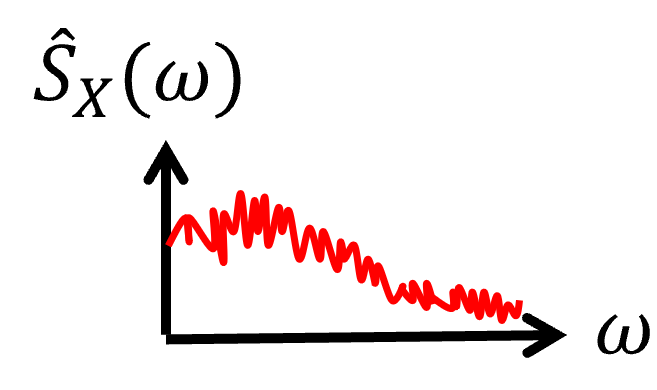
\includegraphics[scale=0.7]{Figuras/fluct.png}
    \end{figure}
\end{enumerate}

\subsection{Periodograma Modificado}
Métodos que modifican el periodograma clásico, para resolver los problemas estacionarios:
\begin{enumerate}
    \item Periodograma modificada (uso de ventanas)
    $$\hat{S}_{MP}(\omega)=\frac{1}{N\cdot U}\bigg| \sum_{n=0}^{N-1} x[n]\omega[n]e^{-j\omega n} \bigg| ^2 $$
    donde $\omega[n]$: ventana en el dominio del tiempo.
    $$U=\frac{1}{N}\sum_{n=0}^{N-1}|\omega[n]|^2 \quad \text{: factor de escala}$$
    
    \item Método de Bartlett (promedio de periodogramas)
    \begin{figure}[H]
    \centering
    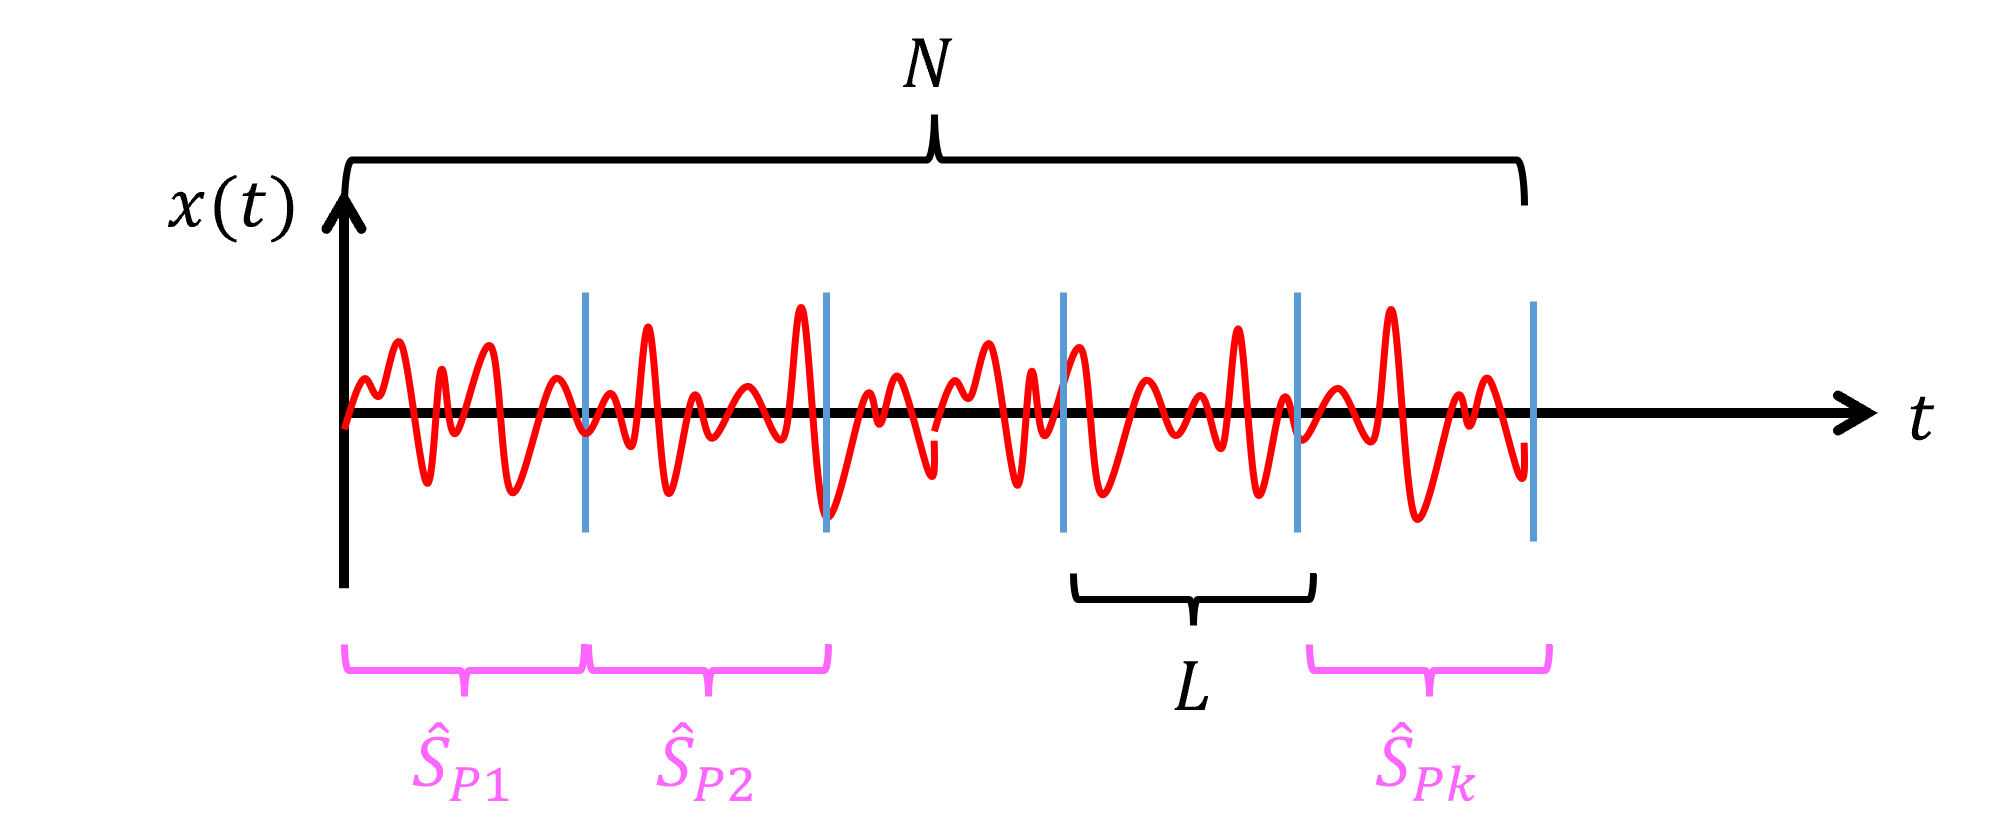
\includegraphics[scale=0.7]{Figuras/ventana1.png}
    \end{figure}
    $$\hat{S}_B(\omega)=\frac{1}{K}\sum_{i=0}^{K-1}\Bigl\{\frac{1}{L}\bigg|\sum_{n=0}^{L-1}x_i[n]e^{-j\omega n} \bigg|^2 \Bigr\} $$
    donde: \begin{itemize}
        \item i: bloque ``i'' de longitud L
        \item K: cantidad de bloques
        \item L: tamaño del bloque
    \end{itemize}
    $$\Longrightarrow  \text{var}\{\hat{S}_X(\omega)\} \approx \frac{1}{K}S_X^2(\omega)$$
    
    
    Problemas:
    \begin{itemize}
        \item Más bloques $\Longrightarrow$ bloques más cortos
        \item Blques cortos $\Longrightarrow$ peor resolución en frecuencia, $\Delta \omega$ es grande.
    \end{itemize}
    $$X[k] = \sum_{n=0}^{L-1}x[n]e^{-j2\pi nk/L} \quad \text{(DFT)}$$
    $\Longrightarrow$ ``Trade-off'': Varianza vs resolución.
    
    \item Método de Welch (promedio de periodogramas con ventanas)
    \begin{figure}[H]
    \centering
    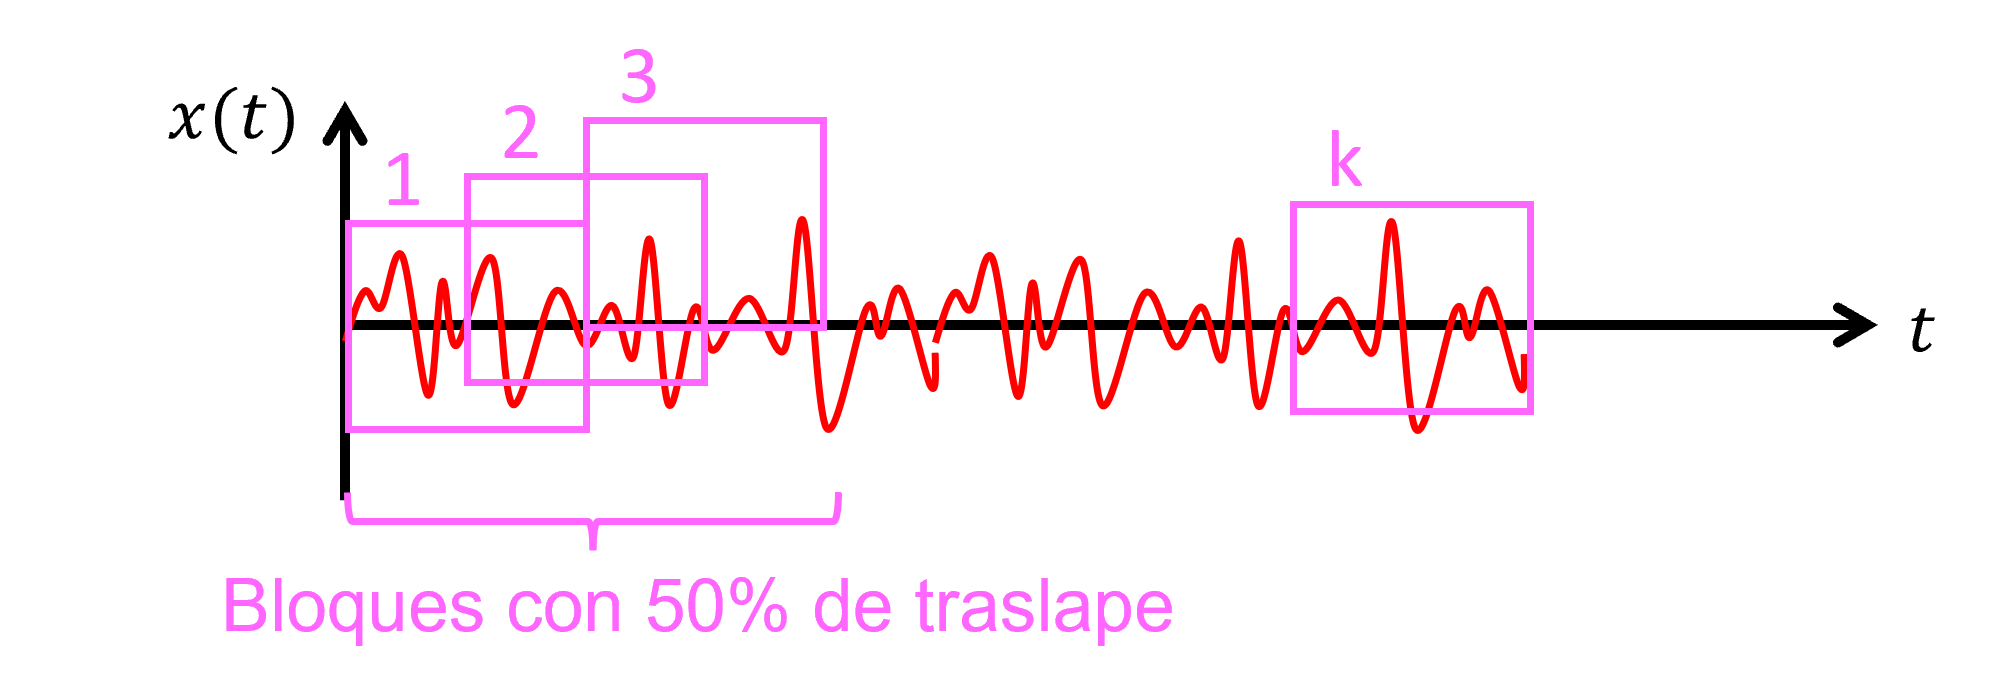
\includegraphics[scale=0.7]{Figuras/ventana2.png}
    \end{figure}
    $$\hat{S}_W(\omega) =\frac{1}{KLU}\sum_{i=0}^{K-1}\bigg| \sum_{n=0}^{L-1} x_i[n]\omega[n]e^{-j\omega n} \bigg|^2$$
    $$\text{var}\{\hat{S}_W(\omega)\} \approx \frac{9}{16}\frac{L}{N}S_x^2(\omega) $$
    Recomendación: En Matlab: \texttt{cpsd()}: cross power spectral density (método de Welch)
    
    \item Método de Blackman-Tucky
    
    
\end{enumerate}

\end{document}
